% Technische Universität Dresden
% Fakultät Informatik
% Institut für Software- und Multimediatechnik
% Seniorprofessur für Multimediatechnik
%
% Example document demonstrating the usage of mmthesis.sty
% 2012-10-26 Andreas Rümpel
% 
% ### build hints (% = filename of tex file) ###
% pdflatex: pdflatex %.tex
% biber: biber % (biber is a modern backend for bibtex, http://biblatex-biber.sourceforge.net)
% glossaries and acronyms: makeglossaries %
%
% Das LATEX2e-Sündenregister: ftp://ftp.dante.de/tex-archive/info/l2tabu/german/l2tabu.pdf
% KOMAScript-Guide: ftp://ftp.dante.de/tex-archive/macros/latex/contrib/koma-script/scrguide.påådf
% Einige typographische Grundregeln und ihre Umsetzung in LaTeX: http://www2.informatik.hu-berlin.de/sv/lehre/typographie.pdf

\documentclass[
	headsepline,
	footsepline,
	fontsize=12pt,
	%draft, % use this for finding overfull boxes
	%parskip, % use this for alternative paragraph formatting
	bibliography=totoc
]{scrbook}

\usepackage{mmthesis}
\usepackage{listings}
\usepackage{color}
\lstset{ %
  backgroundcolor=\color{white},   % choose the background color; you must add \usepackage{color} or \usepackage{xcolor}
  basicstyle=\footnotesize,        % the size of the fonts that are used for the code
  breakatwhitespace=false,         % sets if automatic breaks should only happen at whitespace
  breaklines=true,                 % sets automatic line breaking
  captionpos=b,                    % sets the caption-position to bottom
  %commentstyle=\color{mygreen},    % comment style
  deletekeywords={...},            % if you want to delete keywords from the given language
  escapeinside={\%*}{*)},          % if you want to add LaTeX within your code
  extendedchars=true,              % lets you use non-ASCII characters; for 8-bits encodings only, does not work with UTF-8
  frame=single,                    % adds a frame around the code
  keepspaces=true,                 % keeps spaces in text, useful for keeping indentation of code (possibly needs columns=flexible)
  keywordstyle=\color{blue},       % keyword style
  language=Octave,                 % the language of the code
  morekeywords={*,...},            % if you want to add more keywords to the set
  numbers=left,                    % where to put the line-numbers; possible values are (none, left, right)
  numbersep=5pt,                   % how far the line-numbers are from the code
  %numberstyle=\tiny\color{mygray}, % the style that is used for the line-numbers
  rulecolor=\color{black},         % if not set, the frame-color may be changed on line-breaks within not-black text (e.g. comments (green here))
  showspaces=false,                % show spaces everywhere adding particular underscores; it overrides 'showstringspaces'
  showstringspaces=false,          % underline spaces within strings only
  showtabs=false,                  % show tabs within strings adding particular underscores
  stepnumber=2,                    % the step between two line-numbers. If it's 1, each line will be numbered
  stringstyle=\color{gray},     % string literal style
  tabsize=2,                       % sets default tabsize to 2 spaces
  title=\lstname                   % show the filename of files included with \lstinputlisting; also try caption instead of title
}
% \usepackage{showkeys} % used to show labels
\addbibresource{library.bib} % put name of bib file here with extension

%### switches
%\printoutput % make link colors black, leave deactivated for screen output

%### define metadata
\mmtype{Diplomarbeit} %Diplomarbeit|Großer Beleg|Bachelorarbeit|Masterarbeit|Seminararbeit
\mmtitle{Semantik-gestütztes Hilfesystem für ein komposites Informationsvisualisierungssystem}
\mmtshorttitle{Hilfesystem für komposite InfoVis}
\mmtauthor{Nikolaus Piccolotto}
\mmtsubmissionmonth{November 2013}
\mmtsubmissiondate{30. November 2013}
\mmtsupervisor{Dipl.-Medieninf. Martin Voigt}
%\mmtsupervisorii{Dipl.-Medieninf. Foo Bar} % Co-supervisor, optional

\mmthypersetup % has to be called after setting metadata

%### acronyms
\newacronym{PDF}{PDF}{Portable Document Format}
\newacronym{RCP}{RCP}{Rich Client Platform}
\newacronym{RIA}{RIA}{Rich Internet Application}
\newacronym{RELAXNG}{RELAX NG}{Regular Language Description for XML New Generation}
\newacronym{SGML}{SGML}{Standard Generalized Markup Language}
\newacronym{SWT}{SWT}{Standard Widget Toolkit}
\newacronym{WDC}{W3C}{World Wide Web Consortium}
\newacronym{WPF}{WPF}{Windows Presentation Foundation}
\newacronym{XPath}{XPath}{XML Path Language}
\newacronym{XHTML}{XHTML}{Extensible Hypertext Markup Language}
\newacronym{XML}{XML}{Extensible Markup Language}
% my acronyms
\newacronym{InfoVis}{InfoVis}{Informationsvisualisierung}

\begin{document}
\frontmatter
\pagenumbering{Roman}
\mmtfrontmatter

\listoffigures
\listoftables
\printglossary[type=\acronymtype,style=long,title=Abkürzungsverzeichnis,toctitle=Abkürzungsverzeichnis]
%\printglossary %Glossar

\mainmatter

% ###################################################
\chapter{Einleitung}
\label{chapter:einleitung}

% Einleitung - viele semantische Daten, diese sind sehr nützlich

Im Laufe der letzten Jahre wurden immer mehr semantische Daten veröffentlicht, sowohl in Community-Projekten wie der DBpedia\footnote{\url{http://dbpedia.org}} als auch als Teil der Open Data bzw. Open Government Bewegung, wie z.\,B. data.gov.uk\footnote{\url{http://data.gov.uk/data/search?q=rdf}}. Diese Datenkataloge können von großem Nutzen für jeden sein. Die DBpedia ist eine maschinenlesbare Version der Wikipedia, mit ihr können mit Hilfe der Abfragesprache SPARQL automatisch Fragen beantwortet werden, deren manuelle Recherche zu aufwändig wäre. In data.gov.uk finden sich Informationen, die für alle Steuerzahler im Vereinigten Königreich relevant sein können, wie z.\,B. Organigramme und Gehälter von Regierungsorganisationen.

% ###################################################
\section{Motivation}
\label{section:einleitung:motivation}

% Motivation - es gibt keine gute Möglichkeit, das Wissen in den Daten aufzunehmen. 

% expertenwissen informatik

Jedoch ist es sehr schwierig, das Wissen in den Datenkatalogen aufzunehmen. Wird wie im Falle der DBpedia eine API in Form eines SPARQL Endpoints zur Verfügung gestellt, müssen sowohl die Abfragesprache SPARQL als auch Konzepte von semantischen Daten wie z.\,B. Tripel, Klassen oder Vererbung bekannt sein, um an die Daten zu kommen. Erlaubt das Portal einen Download der Daten, stellt sich die Frage, wie sie geöffnet werden. Gängige Datenverarbeitungstools wie Excel oder Visualisierungstools wie Tableau unterstützen keine semantischen Daten. Es existieren zwar Visualisierungstools für semantische Daten wie Protégé/Jambalaya, diese stellen aber oft nur einen Graphen dar. Die Visualisierung als Netzwerk kann wie im Fall von Organigrammen angebracht sein, aber bei Daten über Aktienkurse wäre ein Liniendiagramm vielleicht besser geeignet.

% expertenwissen visualisierung

Selbst wenn ein Visualisierungstool für semantische Daten existierte, welches verschiedene Arten von Diagrammen unterstützt, würde ein Anwender das Wissen in den Datenkatalogen nicht angemessen vermittelt bekommen. Die Konfiguration von Diagrammen setzt Expertenwissen im Bereich der Informationsvisualisierung voraus, die in den meisten Fällen nicht gegeben ist. Wie viele Farben können in einem Diagramm unterschieden werden? Wie viele Balken sind zu viele für ein Balkendiagramm? Welche Informationen werden am Besten als Farbe kodiert, welche als Größe oder Position?

% vizboard to the rescue

Diese Probleme zu lösen ist das Ziel des Forschungsprojekts VizBoard. Es setzt einen Prozess aus fünf Schritten ein (Abbildung~\ref{figure:vizboard_workflow}): Zuerst wird ein Datensatz hochgeladen (1), danach Konzepte zur Visualisierung ausgewählt (3), Daten im Detail und Visualisierungen gewählt (5), Visualisierungen konfiguriert (7) und schließlich werden die Visualisierungen angezeigt (9).

\begin{figure}[htbp]
	\centering
	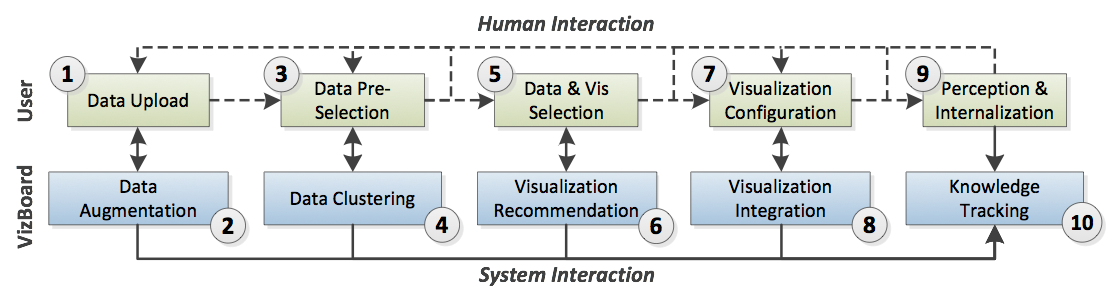
\includegraphics[width=0.75\textwidth]{images/vizboard_workflow.png}
	\caption{VizBoard Workflow}
	\label{figure:vizboard_workflow}
\end{figure}

% ###################################################
\section{Problemstellung und Zielsetzung}
\label{section:einleitung:problemstellung}

% problem liegt im letzten teil

% welche probleme? Visualisierungen auseinanderhalten und einordnen können (intro), visualisierungen bedienen können (bedienung), fragen über daten stellen können (kommentare), konzept der zusammenarbeit von komponenten verstehen (kommunikation), fehler melden können (Feedback), unbekannte konzepte beschrieben bekommen (verlinkung)

Am Ende des VizBoard Workflows angekommen, wird dem Benutzer ein Mashup aus verschiedenen Informationsvisualisierungskomponenten präsentiert, welche miteinander kommunizieren können und so zusammenarbeiten. Beispielsweise aktualisiert sich das Balkendiagramm dem aktuellen Ausschnitt der Karte entsprechend.

Einen unerfahrenen Nutzer, der den Inhalt der Daten verstehen will, stellt diese Situation vor einige Probleme. Zunächst wird er von mehreren verschiedenen Fenstern \enquote{überrumpelt}, die er alle nach der Reihe inspizieren muss. Er muss herausfinden, was sie darstellen und wie sie interpretiert werden sollen. Außerdem werden keine Angaben über die Bedienung gemacht: Welche Elemente lösen Aktionen aus und welche? Wie werden sie aktiviert? Gibt es Alternativen? Während er herumprobiert, um das alles herauszufinden, ändert sich die UI in anderen Komponenten -- ohne dass explizit mit ihnen interagiert wurde. Wann und nach welchen Regeln passiert das? Wenn der Benutzer die Daten inspiziert, werden einige Fragen auftauchen. Was bedeutet ein bestimmter Begriff? Wie ist diese Metrik definiert? Warum fällt sie in diesem einen Jahr so deutlich ab? 

% ziel der arbeit: hilfesystem konzept, prototypisch umsetzen, aber quasi "real-world" prototyp. kein paper mockup.

Ziel dieser Arbeit ist die Entwicklung eines Konzepts für ein semantik-gestütztes Hilfesystem für VizBoard, welches unerfahrenen Nutzer den Umgang mit dem Visualisierungs-Mashup erleichtert. Dadurch soll deren Verständnisprozess möglichst nicht unterbrochen werden, sodass sie möglichst schnell die Erkenntnisse finden, die sie gesucht haben. Das erarbeitete Konzept soll prototypisch umgesetzt und in CRUISe, welches die Basis für VizBoard ist, integriert werden.

% teilziele der arbeit
% szenario
% anforderungsanalyse
% grundlagen zu den betroffenen themen, also infovis, semantische daten, user assistance
% schauen was andere so gemacht haben und wie es genutzt werden kann
% konzept erstellen
% prototypen implementieren
% evaluation mit nutzerstudie

Daraus leiten sich die folgenden Teilziele der Arbeit ab: Jop. Genau.

% ###################################################
\section{Aufbau der Arbeit}
\label{section:einleitung:aufbau}

% Aufbau der Arbeit erklären, kommt zum Schluss

% ###################################################
\chapter{Stand der Forschung und Technik}
\label{chapter:standderforschung}

Der folgende Abschnitt besteht aus drei Teilen. Zuerst wird die Aufgabenstellung in einem Szenario verdeutlicht (Abschnitt~\ref{section:standderforschung:szenario}). Daraus werden Anforderungen an das Hilfesystem abgeleitet (Abschnitt~\ref{section:standderforschung:anforderungsanalyse}) und danach die Grundlagen von semantischen Daten, Informationsvisualisierungen und Software Support erläutert (Abschnitt~\ref{section:standderforschung:grundlagen}).

% ###################################################
\section{Szenario}
\label{section:standderforschung:szenario}

% kurze einleitung noch mal

Wie in Kapitel~\ref{chapter:einleitung} erläutert, ist das komposite InfoVis-System Teil der webbasierten Anwendung VizBoard. Sie leitet den Benutzer in mehreren Schritten von der Auswahl eines Datensatzes zur finalen, kompositen Informationsvisualisierung. Im vorletzten Schritt wählt dieser mit Hilfe eines Facettenbrowsers geeignete Visualisierungskomponenten aus, welche danach angezeigt werden. Um die Problemstellung noch einmal zu verdeutlichen, wird im folgenden ein mögliches Szenario beschrieben.

% einführung der problemstellung
Anna möchte für ihr Biologiestudium mehr über die geografische Verteilung verschiedener Genvarationen herausfinden. Dazu sucht sie im Internet nach einem Datensatz, welchen sie auch findet. 
% unbekanntes format, kann es nirgends ordentlich öffen und selbst wenn es in excel ginge, wüsste sie nicht, welche charts sie am besten erstellen sollte
Leider ist er in einem für Anna unbekannten Format abgespeichert, nämlich OWL. Sie versucht die Datei mit Microsoft Excel und SPSS zu öffnen, weil sie keine anderen Programme zur Datenverarbeitung kennt, aber scheitert. Anna stellt fest, dass nur ihr Texteditor OWL öffnen und vernünftig darstellen kann. Als sie die Datei überfliegt, kann sie den Inhalt zwar erahnen, aber es ist einfach zu viel Text um ihn vollständig zu lesen. Davon abgesehen sind geografische Breite und Länge als Zahlenkombination keine anschauliche Repräsentation von Orten, auch Verteilungen von Werten sind so schwer ersichtlich. Anna würde viel Zeit aufwenden müssen um sehr wenig des Inhalts zu verstehen. Aber selbst wenn sie die Datei in Excel hätte öffnen können, hätte sie nicht gewusst, mit welchen Diagrammen die vorhandenen Daten am Besten verstanden würden. Anna hört von einem Freund, dass VizBoard gut geeignet ist, um semantische Datensätze anzusehen und probiert es aus.

% Der Benutzer ist laut unserem Rollenmodell weder Developer noch Visualisierungsexperte, d.h. er hat erstmal Schwierigkeiten zu erfassen, was hier überhaupt abgeht

Anna hat ihren Datensatz auch bei VizBoard gefunden und ist neugierig: Sie wählt eine Karte, ein Balkendiagramm, eine Tabelle und eine Treemap aus (Abbildung~\ref{figure:szenario-skizze}); kurz darauf werden ihr die Visualisierungskomponenten angezeigt. Anna benutzt VizBoard zum ersten Mal und macht außer Facebook und YouTube auch sonst nicht viel im Internet, das heißt sie ist zunächst von den vier unterschiedlichen Fenstern etwas überfordert.

\begin{figure}[htbp]
	\centering
	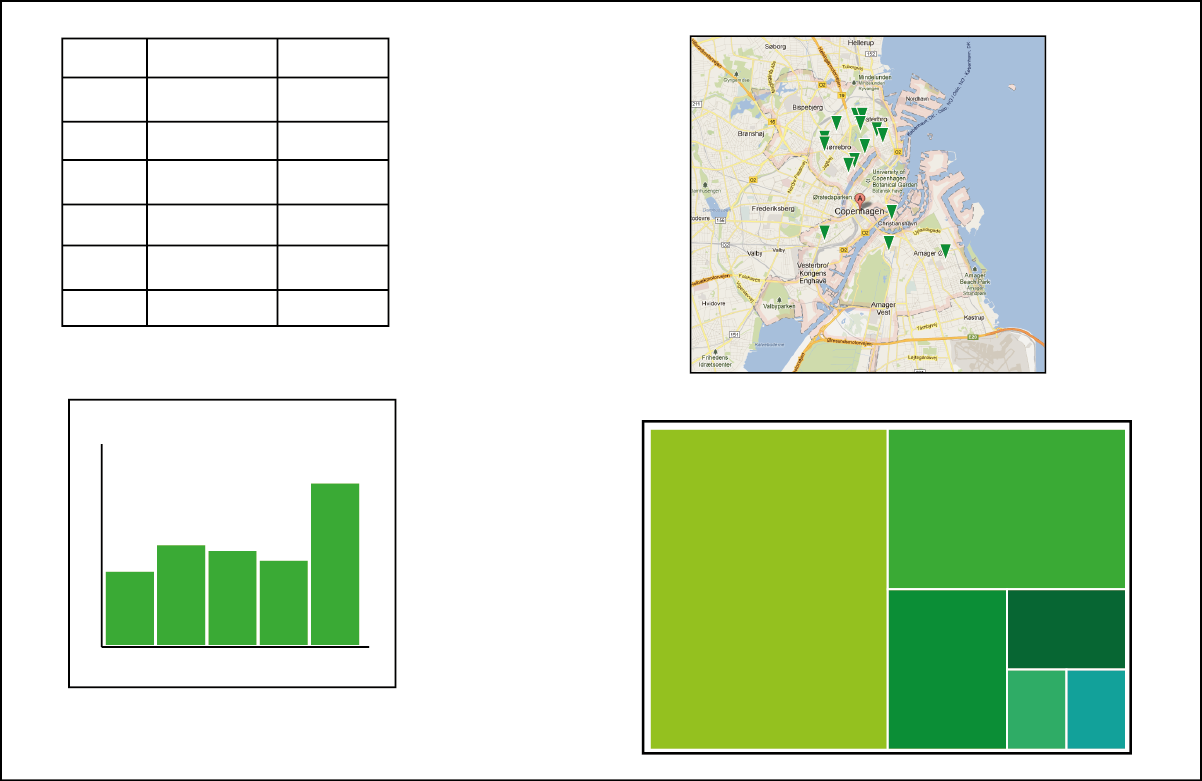
\includegraphics[width=0.75\textwidth]{images/szenario-skizze.png}
	\caption{Skizze der VizBoard Visualisierungskomponenten}
	\label{figure:szenario-skizze}
\end{figure}

VizBoard bietet Anna aber sofort eine einführende Übersicht und erklärt kurz die Darstellungsform und den Inhalt jeder Komponente. Eine denkbare Erklärung der Treemap wäre zum Beispiel:

\begin{quote}
Eine Treemap ist eine hierarchische Visualisierung, um Größenverhältnisse anschaulich zu machen. In dieser werden die Anzahl von Genvariationen pro geografischer Region dargestellt.
\end{quote}

% Was sind das für Fenster? Welche Komponente ist welche? Welche macht was? Wie kann ich sie bedienen? HUUUPS da ändert sich ja was obwohl ich dort nix gemacht hab! Wie hängen die zusammen? Was sind das für Daten, die dargestellt werden? 

Damit bekommt Anna einen Überblick über die verfügbaren Visualisierungen und weiß, welches Fenster welche Visualisierung enthält und für was diese gut sind. Nun möchte sie die Tabelle, in der die durch die Treemap visualisierten Daten stehen, nach der Spalte \enquote{Anzahl} sortieren. Anna sieht aber nicht, wie sie das machen soll, da in der Tabelle kein offensichtliches Kontrollelement wie z.\,B. ein Button vorhanden ist. Sie bemerkt ein Fragezeichen in der Titelleiste des Fensters und klickt darauf. Der verfügbare Viewport wird abgedunkelt und es erscheint ein neues Fenster, welches die verfügbaren Aktionen mit Hilfe von Text, Bildern und Animationen erklärt. Anna lernt, dass sie mit einem einfachen Linksklick auf den jeweiligen Kopf einer Tabellenspalte nach dieser sortieren kann und außerdem eine oder mehrere Zeilen auswählen kann. Sie sortiert die Tabelle wie gewollt und wählt die ersten drei Zeilen aus. Plötzlich verkleinert die Karte ihr Zoomlevel und Anna ist verwirrt: Sie hat nur mit der Tabelle interagiert und es bestand keine sichtbare Verbindung zwischen den beiden Fenstern. Allerdings wurde nach der Zeilenauswahl ein Pfeil von der Tabelle zur Karte gezeichnet, welcher mit einem Icon in Form eines Briefes versehen ist. Anna vermutet, dass doch irgendeine Verbindung zwischen den beiden Visualisierungen besteht und klickt auf den Brief. Ähnlich wie vorhin bei der Hilfe zur Tabelle wird der Viewport abgedunkelt und ein neues Fenster wird eingeblendet. Es erklärt die Kommunikation zwischen den Visualisierungen mit Hilfe von Animationen, Text und Bildern. Nun weiß Anna auch, wie die verschiedenen Fenster zusammenhängen und kann sich ihrer eigentlichen Aufgabe widmen.

% Was heißt GDP? Wie wird das berechnet? Was soll die Spitze bei 1990? Woher kommt die? Diese eine Komponente scheint kaputt zu sein, wo kann ich mich beschweren?

In der Tabelle findet sie auch eine Spalte \enquote{SNP}. Anna weiß zwar, dass sie die Abkürzung schon einmal gesehen hat, kennt aber im Moment ihre Bedeutung nicht. Praktischerweise ist der Spaltenkopf mit der Wikipedia verlinkt und sie wird sofort auf die entsprechende Seite weitergeleitet. Anna erinnert sich, dass \enquote{SNP} \enquote{Single-nucleotide polymorphism} bedeutet und sie bekommt auch gleich zusätzliche Informationen zu diesem Thema. Sie widmet sich weiter der Tabelle und stellt fest, dass die Ortsbezeichnung \enquote{Kopenhagen} nicht mit der Markierung in der Karte übereinstimmt. Außerdem ist sie erstaunt, wie hoch die Verbreitung eines bestimmten SNPs dort ist und würde gerne die Ursache dafür wissen. In der Hilfe zur Tabelle wurde sie auch über die Möglichkeit, Kommentare an den Daten vorzunehmen, aufgeklärt. Anna kommentiert sowohl die falschen Geokoordinaten als auch ihre Frage über die Verbreitung des SNPs, sodass sie später über Antworten informiert wird. Nun kann Anna sich mit der vierten Visualisierung, dem Balkendiagramm, beschäftigen. Allerdings reagiert es auf keine Mausklicks und macht auch sonst nicht den Eindruck, die Daten akkurat darzustellen. Anna meldet die kaputte Visualisierung über die eingebaute Feedback-Funktion und schließt das Fenster, um sich den anderen drei Visualisierungskomponenten zuzuwenden.

% ###################################################
\section{Anforderungsanalyse}
\label{section:standderforschung:anforderungsanalyse}

Aus dem Szenario (Kapitel~\ref{section:standderforschung:szenario}) lassen sich nun verschiedene Anforderungen an ein Hilfesystem für komposite Informationsvisualisierungssysteme ableiten.

\subsection{Funktionale Anforderungen}
\label{section:standderforschung:anforderungsanalyse:funktionale_anforderungen}

Blabla

\begin{itemize}
	\item\textbf{Intro}: Das Hilfesystem soll einen kurzen Überblick über das InfoVis-System geben und Darstellungsform sowie Inhalt jeder Komponente kurz erläutern.
	\item\textbf{Bedienung}: Das Hilfesystem soll erklären können, wie eine Komponente bedient wird. Diese Informationen umfassen beispielsweise welche Operationen welche Aktionen (eventuell auf welchen Daten) ausführen.
	\item\textbf{Feedback}: Fehler in Komponenten sollen über ein Feedback-System gemeldet werden können.
	\item\textbf{Verlinkung}: Das Hilfesystem soll nicht-triviale Begriffe mit einer Wissensbasis‚ verlinken, sodass nicht nur auf die Begriffsbedeutung hingewiesen werden, sondern dem Benutzer auch zusätzliche Informationen zur Verfügung gestellt werden können.
	\item\textbf{Kommunikation}: Das Hilfesystem soll erklären können, wie gegebene Komponenten miteinander kommunizieren.
	\item\textbf{Kommentare}: Der Benutzer soll die Möglichkeit haben Daten zu kommentieren und Bereiche der Visualisierung zu markieren und mit ebenfalls mit einem Kommentar zu versehen, sodass auch auf fehlende Daten hingewiesen werden kann.
\end{itemize}

% was muss also ins related work?
% wie der wissensaufnahmeprozess funktioniert, weil ich ja erklärungen gebe, speziell planerklärung
% was es so für infovis gibt, weil ich mit denen arbeite
% was es so für hilfekonzepte gibt, weil es das ist was ich tue
% social web, weil kommentare implementiert werden

\subsection{Nichtfunktionale Anforderungen}
\label{section:standderforschung:anforderungsanalyse:nichtfunktionale_anforderungen}

Bla bla

\begin{itemize}
	\item\textbf{Korrektheit}: Eine gegebene Hilfestellung darf keine Fehlinformationen enthalten, weil sie sonst mehr verwirrt als hilft.
	\item\textbf{Vollständigkeit}: Eine gegebene Hilfestellung muss alle Informationen enthalten, die der Nutzer benötigt um danach seine gewünschte Aufgabe ausführen zu können.
	\item\textbf{Verständlichkeit}: Hilfestellungen müssen in einer Form präsentiert werden, die der Benutzer schnell und mit geringem mentalen Aufwand verarbeiten kann.
	\item\textbf{Einheitlichkeit}: Das Look \& Feel von Teilen des Hilfesystems (z.B. Kommentare) muss komponentenübergreifend einheitlich sein, damit der Benutzer einmal gelerntes wiederverwenden kann.
	\item\textbf{Minimalität}: Der Komponentenentwickler soll seine Komponente mit möglichst wenig Aufwand zum Hilfesystem kompatibel machen können, ansonsten werden nur sehr wenige Komponenten -- und damit der Benutzer -- davon profitieren.
	\item\textbf{Universalität}: Das Hilfesystem soll für alle Komponenten und Visualisierungen in gleicher Qualität funktionieren.
	\item\textbf{Wiederverwendbarkeit}: Die Kommentare sollen möglichst in allen Visualisierungen wiederverwendet werden, damit viele Benutzer von den Erkenntnissen anderer profitieren können.
	\item\textbf{Unaufdringlichkeit}: Das Hilfesystem soll den Benutzer nicht von seinen Aufgaben ablenken und nur auf Anfrage zum Einsatz kommen oder es soll selbständig erkennen, wenn der Benutzer Hilfe benötigt.
\end{itemize}

% ###################################################
\section{Grundlagen}
\label{section:standderforschung:grundlagen}

Hurrrrr derp herp

\subsection{CRUISe, EDYRA \& VizBoard}
\label{section:standderforschung:grundlagen:cruise_vizboard}

% grundlagen von cruise edyra vizboard. wichtig weil mein hilfesystem dort eingesetzt wird
CRUISe \cite{Pietschmann2009, Pietschmann2012} ist ein Framework zur Konstruktion von webbasierten, kompositen User Interfaces (auch Mashups). Diese bestehen aus mehreren voneinander unabhängigen, wiederverwendbaren User Interface Services (z.\,B. eine Karte, eine Tabelle und ein Kalender) welche zur Laufzeit hinzugefügt, konfiguriert und ausgetauscht werden können. Abbildung~\ref{figure:cruise_architektur} zeigt die Architektur von CRUISe. Zuerst werden Komponenten von Entwicklern erstellt und modelliert (1). Danach interpretiert CRUISe das Kompositionsmodell (2), matcht es gegen die Kontextanforderungen (3), bildet ein Ranking (4) und integriert schließlich die am besten geeignete Komponente ins User Interface (5).

\begin{figure}[htbp]
	\centering
	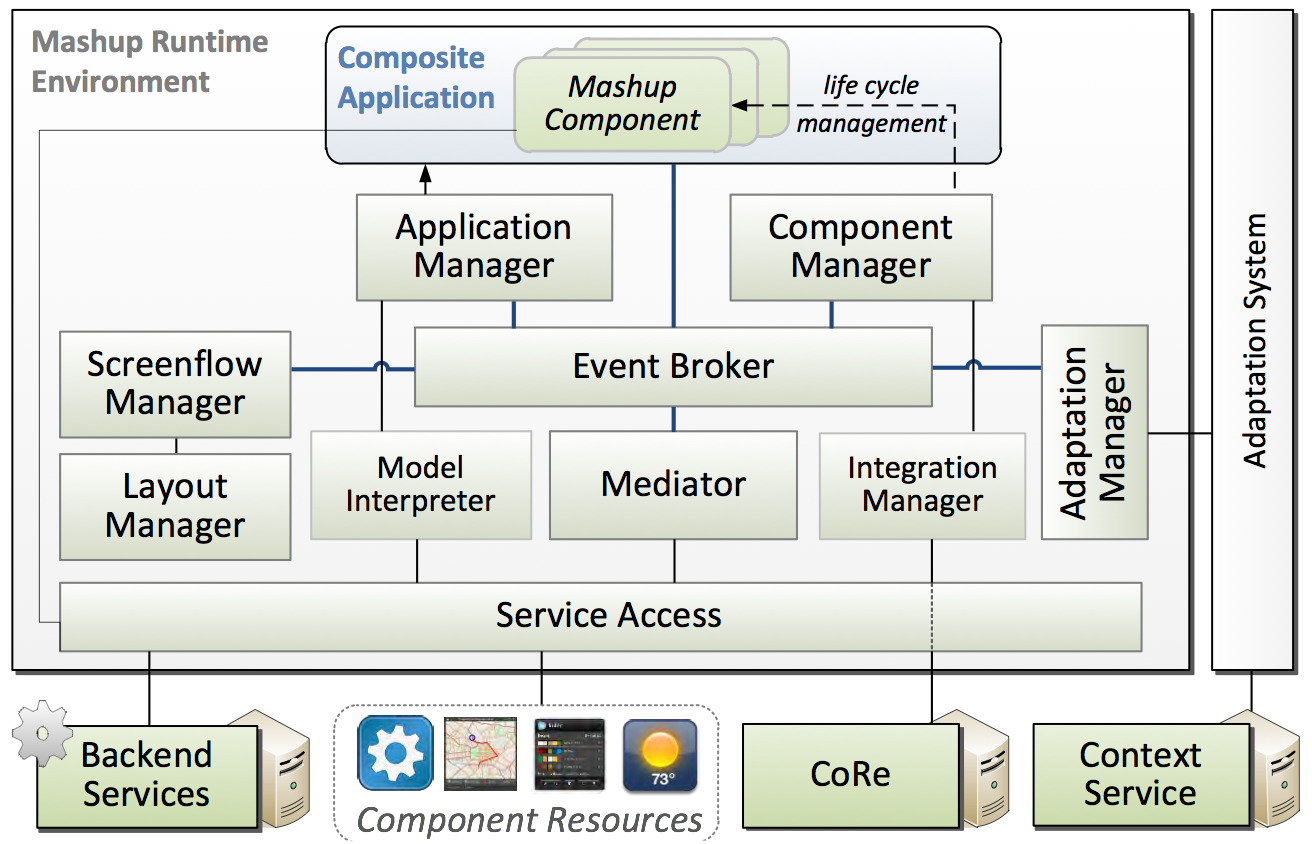
\includegraphics[width=0.75\textwidth]{images/grundlagen-cruise_architektur.png}
	\caption{CRUISe Architektur aus \cite{Pietschmann2012}}
	\label{figure:cruise_architektur}
\end{figure}

CRUISe geht davon aus, dass professionelle Softwarentwickler Komponenten zu kompositen Sichten modellieren, welche dann von Endnutzern nur noch aufgerufen werden. EDYRA \cite{Ruempel2011} greift auf das CRUISe Framework zurück, um es Endnutzern selbst zu ermöglichen, diese Aufgabe auszuführen. Dazu schlägt EDYRA zur Laufzeit Komponenten vor, welche sofort integriert oder gelöscht werden können.

VizBoard \cite{Voigt2013} benutzt das CRUISe Framework, um Endnutzern die Möglichkeit zu geben, semantische Datensätze mit Hilfe verschiedener InfoVis verstehen zu können. Abbildung~\ref{figure:vizboard_architektur} zeigt die Architektur von VizBoard. Die Daten werden zuerst aus verschiedenen Quellen in eine semantische Repräsentation konvertiert und im Data Repository (DaRe, 1) gespeichert. Das Component Repository (CoRe, 3) verwaltet die verschiedenen Visualisierungskomponenten (2) und ist für Matching und Ranking von Komponenten zuständig, bevor sie in der Runtime (4) integriert werden. Sowohl das DaRe als auch das CoRe greifen auf die Visualization Ontology (VISO, 5) zurück, die Wissen über verschiedene Aspekte von Visualisierungen, wie z.\,B. Struktur der visualisierten Daten, Mapping der Daten auf visuelle Attribute oder Interaktionsmöglichkeiten, enthält \cite{Polowinski2013}.
% architekturbild --> vizboard paper

\begin{figure}[htbp]
	\centering
	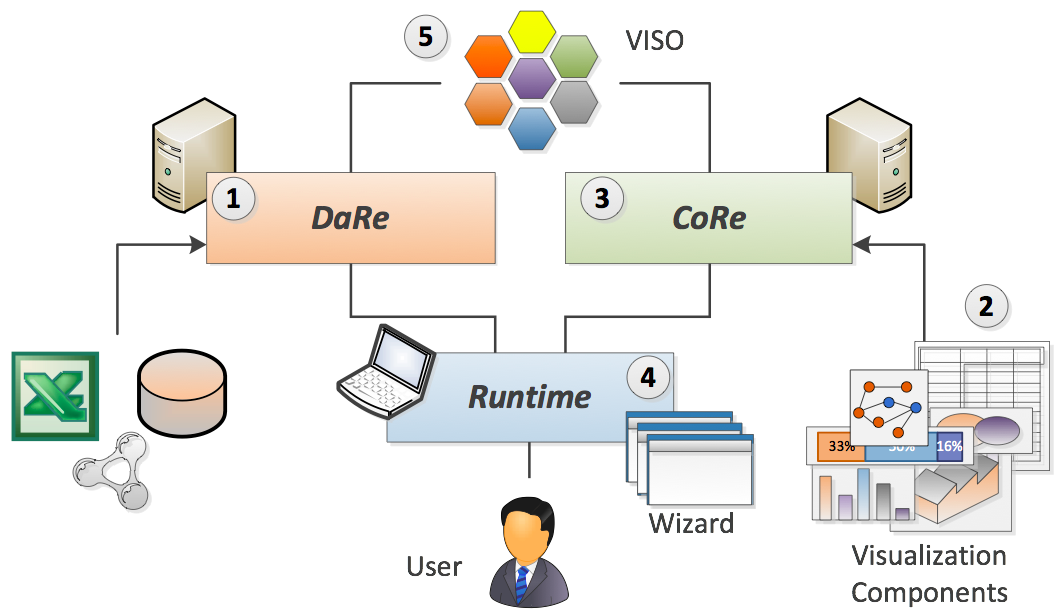
\includegraphics[width=0.75\textwidth]{images/grundlagen-vizboard_architektur.png}
	\caption{VizBoard Architektur aus \cite{Voigt2013}}
	\label{figure:vizboard_architektur}
\end{figure}

\subsubsection{Data Repository}
\label{section:standderforschung_data_repository}

% dare --> vizboard paper, beleg
Im DaRe werden Daten aus verschiedenen Quellen in einer semantischen Repräsentation gespeichert. Dabei durchläuft das DaRe verschiedene Phasen (Abbildung~\ref{figure:dare_phasen}). Zuerst wird der Datensatz \emph{analysiert} und Metainformationen gesammelt, beispielsweise werden Subklassen gezählt und wichtige Konzepte identifiziert. Diese werden an den Datensatz \emph{annotiert}. Zur Laufzeit müssen diese Erkenntnisse wieder aus dem Datensatz \emph{extrahiert} werden. Das DaRe stellt eine REST API zur Verfügung, über die ein Datensatz abgerufen werden kann \cite{Piccolotto2012}.

\subsubsection{Komponentenbeschreibung}
\label{section:standderforschung:grundlagen:cruise_vizboard:komponentenbeschreibung}

% komponentenbeschreibung 5.1.3
Komponenten in CRUISe werden generisch und einheitlich durch Properties, Events und Operationen sowie Metainformationen beschrieben. Properties geben Auskunft über den Zustand einer Komponente, also beispielsweise Breite und Höhe oder die Sortierreihenfolge der Elemente. Events weisen andere Komponenten auf interne Zustandsänderungen hin, zum Beispiel wenn sich die Sortierreihenfolge geändert hat. Operationen sind Methoden einer Komponente, die durch Events ausgelöst werden, z.\,B. \texttt{reassignNumbers(order)}, um die Nummerierung der Pins in einer Karte anzupassen. Zu den Metainformationen gehören u.\,a. der Name einer Komponente oder der Preis.

\subsubsection{Kommunikationsmodell}
\label{section:standderforschung:grundlagen:cruise_vizboard:kommunikationsmodell}

% kommunikationsmodell 5.2.2
Die Kommunikation von Komponenten untereinander ist ereignisgesteuert, d.\,h. eine Komponente veröffentlicht ein Event, dessen Nachricht mit Hilfe des Publish/Subscribe Paradigma an alle Subscriber in diesem Kanal (Link) übertragen wird. Subscriber reagieren auf das Event, indem sie bestimmte Operationen ausführen. Die Übertragung der Nachrichten wird durch sogenannte Links umgesetzt, welche $n$ Events mit $m$ Operationen verbinden. Spezielle Links sind Backlinks, die eine Zweiwegekommunikation zwischen Komponenten ermöglichen und PropertyLinks, die Properties synchron halten. Ein Überblick über die verschiedenen Links ist in Abbildung~\ref{figure:cruise_links} zu sehen.

\begin{figure}[htbp]
	\centering
	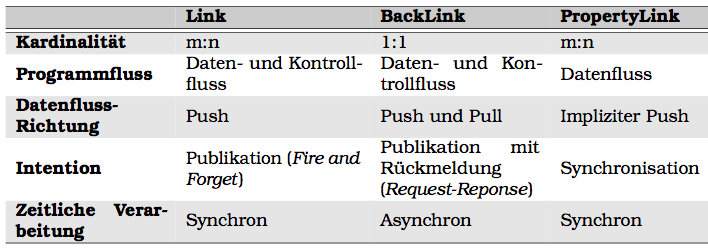
\includegraphics[width=0.75\textwidth]{images/grundlagen-cruise_links.png}
	\caption{CRUISe Links aus \cite{Pietschmann2012}}
	\label{figure:cruise_links}
\end{figure}

\subsubsection{Laufzeitumgebung}
\label{section:standderforschung:grundlagen:cruise_vizboard:laufzeitumgebung}

Die Laufzeitumgebung (Mashup Runtime Environment, MRE) ist für die Ausführung und Verwaltung der kompositen Anwendung verantwortlich und besteht aus mehreren Modulen (Abbildung~\ref{figure:cruise_mre}).

% laufzeitumgebung (tsr) 6.2, 7.2.2
\begin{figure}[htbp]
	\centering
	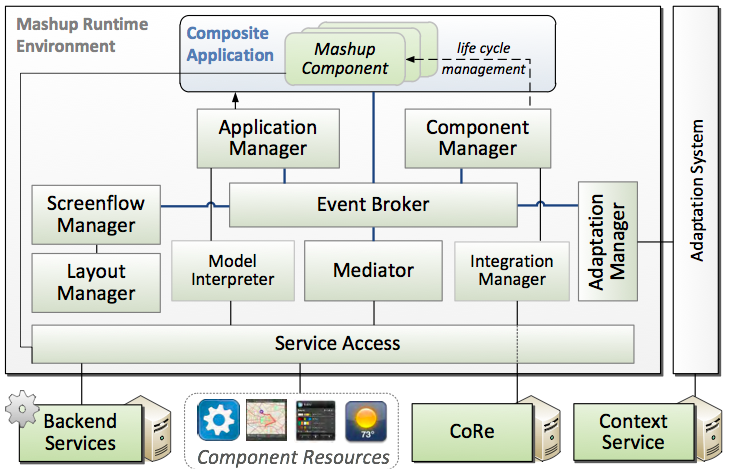
\includegraphics[width=0.75\textwidth]{images/grundlagen-cruise_mre.png}
	\caption{Mashup Runtime Environment Architektur aus \cite{Pietschmann2012}}
	\label{figure:cruise_mre}
\end{figure}

Der \textbf{Application Manager} initialisiert alle anderen Module und ist für die globale Fehlerbehandlung zuständig. Für den Lebenszyklus der einzelnen Komponenten ist der \textbf{Component Manager} zuständig. Die Integration übernimmt allerdings der \textbf{Integration Manager}. Im Mashup Modell definierte Sichten und Übergänge zwischen ihnen werden vom \textbf{Screenflow Manager} interpretiert. Gerendert werden die Komponenten aber vom \textbf{Layout Manager}. Nachrichten zwischen Komponenten der Anwendung und Modulen der MRE werden durch den \textbf{Event Broker} übermittelt. Sind die Parameter von Event und Operation syntaktisch nicht äquivalent, aber semantisch aufeinander abbildbar (z.\,B. zwei gleiche Konzepte aus verschiedenen Namespaces wie \texttt{dbpedia:city} und \texttt{geonames:city}), übernimmt dies der \textbf{Mediator}. Die dynamische Anpassung der Anwendung (z.\,B. von Komponenten, Layout und Kommunikationsmodell) wird gegebenenfalls durch den \textbf{Adaptation Manager} durchgeführt. Der \textbf{Context Service} \cite{Pietschmann2008} speichert Informationen über den Nutzungskontext, beispielsweise den Aufenthaltsort des Nutzers. Letztlich erlaubt das \textbf{Service Access} Modul Zugriff auf Web-Dienste und Ressourcen im Backend.

\subsubsection{VISO}
\label{section:standderforschung:grundlagen:cruise_vizboard:viso}

% viso
In der Visualization Ontology (VISO) ist Visualisierungswissen gespeichert. Sie kann dabei helfen, zur Laufzeit die Domäne dargestellter Daten zu identifizieren oder notwendiges Wissen zur User Assistance (Abschnitt~\ref{section:standderforschung:user_assistance}) zur Komponentenbeschreibung hinzuzufügen. Unter anderem enthält sie folgende Konzepte und deren Verbindungen untereinander:

\begin{itemize}
	\item Visualisierte Daten (\texttt{viso:data})
	\begin{itemize}
		\item Scale of Measurement (nominal, ordinal, quantitativ, unstrukturiert)
		\item Struktur der Daten (tabellarisch, Tripel, verlinkt)
		\item Art der Variable (abhängig, unabhängig, Dimension etc.)
		\item Domäne
	\end{itemize}
	\item Aktivitäten (\texttt{viso:activity})
	\begin{itemize}
		\item Nutzeraktivitäten (Operationen, Aktionen, Aufgaben)
		\item Visualisierungspipeline (Editieren, Visual Mapping, Datentransformation etc.)
	\end{itemize}
	\item Grafikvokabular (\texttt{viso:graphic})
	\begin{itemize}
		\item Visuelle Attribute (Größe, Farbe, Textur etc.)
		\item Koordinaten (kartesisch, Zylinder, Kugel etc.)
		\item Art der grafischen Repräsentation (Karten, Chart mit zwei Achsen, animierte InfoVis etc.)
		\item Beziehungen zwischen Objekten (Clustering, Labeling, verlinkt etc.)
	\end{itemize}
	\item System (\texttt{viso:system})
	\begin{itemize}
		\item Hardware
		\item Software
		\item Bildschirmauflösung
		\item Rundes, eckiges oder unstrukturiertes Display
	\end{itemize}
\end{itemize}

Dieses Wissen wird in VizBoard auf verschiedene Art und Weise genutzt (Abbildung~\ref{figure:viso}). Mit Hilfe der VISO kann Wissen von Visualisierungsexperten formalisiert und im Rankingalgorithmus berücksichtigt werden (2). Gleichermaßen wird sie zur Annotation der Daten im Data Repository (Abschnitt~\ref{section:standderforschung_data_repository}) benutzt (3). Visualisierungskomponenten (4) und Nutzer- bzw. Systemkontext (5) werden durch VISO-Konzepte beschrieben.

\begin{figure}[htbp]
	\centering
	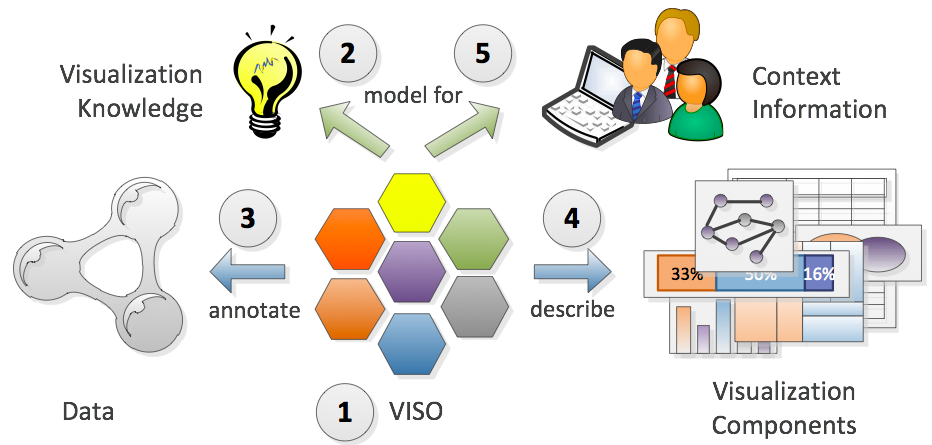
\includegraphics[width=0.75\textwidth]{images/grundlagen-viso.png}
	\caption{Nutzung der VISO in VizBoard}
	\label{figure:viso}
\end{figure}

\subsection{Semantische Datensätze}
\label{section:standderforschung:grundlagen:semantische_daten}

% Grundlagen von RDF, RDFS, OWL. Wichtig weil später Kommentare wieder in einer Ontologie abgelegt werden müssen
Eine Ontologie ist \enquote{an explicit specification of a conceptualization} \cite{Gruber1995} und wird benutzt um domänenspezifisches Wissen abzubilden \cite{Chandrasekaran1999}. Sie besteht aus mehreren Elementen:

\begin{itemize}
	\item Eine Klasse repräsentiert ein Konzept, eine Entität, ein Ding, beispielsweise ein \textit{Smartphone}.
	\item Eine Instanz ist ein konkretes Objekt einer Klasse, zum Beispiel das \textit{iPhone mit der Seriennummer XYZ-ABC}.
	\item Datatype Properties beschreiben eine Instanz näher, zum Beispiel die \textit{Seriennummer} oder \textit{Bildschirmgröße} des iPhones.
	\item Objektattribute beschreiben Beziehungen zwischen Klassen und deren Instanzen, beispielsweise eine Person \textit{besitzt} ein Smartphone.
	\item Außerdem existieren noch Axiome, Regeln, Funktionen und Einschränkungen, welche die Logik einer Ontologie beschreiben.
\end{itemize}

Um eine Ontologie maschinenlesbar darzustellen, hat das World Wide Web Consortium (W3C) verschiedene Beschreibungssprachen eingeführt. Die bekanntesten sind Resource Description Framework (RDF), RDF Schema (RDFS) und Web Ontology Language (OWL). Mit diesen Sprachen lässt sich unterschiedlich viel Semantik u.\,a. in Form von Ontologien, Thesauren oder Vokabularen ausdrücken; die Komplexität der Dokumente und damit der Aufwand, sie zu erstellen, verhalten sich aber direkt proportional (siehe Abbildung~\ref{figure:semantic_spectrum}).

\begin{figure}[htbp]
	\centering
	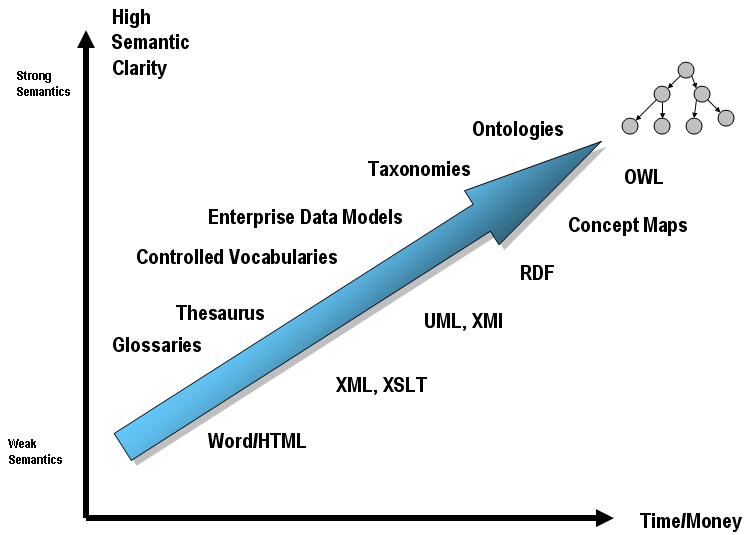
\includegraphics[width=0.75\textwidth]{images/grundlagen-semantic_spectrum.png}
	\caption{Semantic Spectrum \cite{Bergman2007}}
	\label{figure:semantic_spectrum}
\end{figure}

% rdf

RDF ist von den genannten die Sprache mit den wenigsten Features, sie kann nur Tripel der Form (Subjekt, Prädikat, Objekt) darstellen. Die Elemente der Tripel sind Resourcen (durch URIs gekennzeichnet), welche Objekte beschreiben. So drückt der Tripel (\texttt{http://alice.de}, \texttt{http://foaf.de/knows}, \texttt{http://bob.de}) aus, dass das Element \enquote{Alice} mit \enquote{Bob} über die Relation \enquote{knows} verbunden ist. In RDF existieren noch keine Vererbung, Klassen, Properties oder Logik.

% rdfs

RDFS ist eine Erweiterung von RDF, nämlich um Klassen und Vererbung, Datatype Properties und Objektattribute. Allerdings ist RDFS damit noch immer nicht so mächtig wie OWL.

% owl

OWL erweitert wiederum RDFS um einige Konzepte. So können beispielsweise Axiome definiert werden, Attribute können als transitiv oder symmetrisch deklariert werden, es existieren Mengenoperationen und Kardinalitäten und Wertebereiche können eingeschränkt werden. OWL existiert in zwei Versionen, da in den meisten Fällen nicht der volle Funktionsumfang benötigt wird: OWL Lite ist für Anwendungen gedacht, die kaum mehr als eine Klassenhierarchie und Attribute benötigen. OWL-DL ist auf die Logik in der Ontologie fokussiert und wird vor allem für Reasoner eingesetzt, um selbstständig Schlüsse innerhalb des vorgegebenen formalen Systems ziehen zu können. OWL 2 wurde 2009 eingeführt, dieser Standard erweitert OWL zum Beispiel um asymmetrische, reflexive und disjunkte Attribute.

\subsection{Informationsvisualisierung}
\label{section:standderforschung:grundlagen:informationsvisualisierung}

% InfoVis Grundlagen. Wichtig weil das die Komponenten sind, mit denen ich zu tun habe.

Card et al. \cite{Card1999} definieren den Begriff \enquote{Informationsvisualisierung} wie folgt:

\begin{quote}
The use of computer-supported, interactive, visual representations of abstract data to amplify cognition.
\end{quote}

Beispiele dafür sind Balkendiagramme, Treemaps \cite{Shneiderman1992} und Parallel Coordinates \cite{Inselberg1991} (Abbildung~\ref{figure:parallel_coordinates}). Mangels Interaktivität sind Infografiken \cite{Smiciklas2012} von den eben definierten Informationsvisualisierungen ausgeschlossen.

\begin{figure}[htbp]
   \centering
   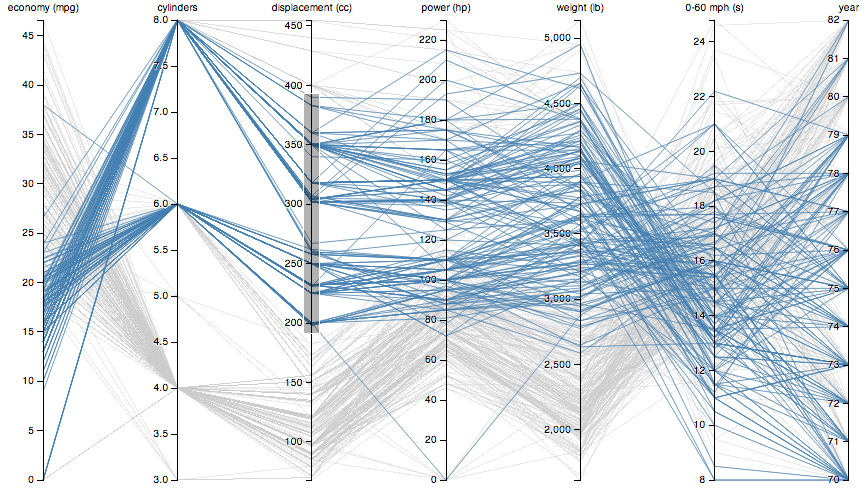
\includegraphics[width=0.5\textwidth]{images/grundlagen-parallel_coordinates.png} 
   \caption{Parallel Coordinates}
   \label{figure:parallel_coordinates}
\end{figure}

% visualisierungsprozess

Informationsvisualisierungen können besonders bei der Exploration großer Datenmengen hilfreich sein \cite{Kohlhammer2011}. Die Wissensaneignung erfolgt dabei iterativ (Abbildung~\ref{figure:visual_analytics_process}). Zuerst werden Daten auf eine Visualisierung gemappt, deren Parameter vom Benutzer geändert werden können. Daraus lernt dieser etwas über die Daten und kann danach (\enquote{Feedback loop}) von vorne anfangen und eine andere Visualisierung wählen oder die Daten transformieren.

\begin{figure}[htbp]
   \centering
   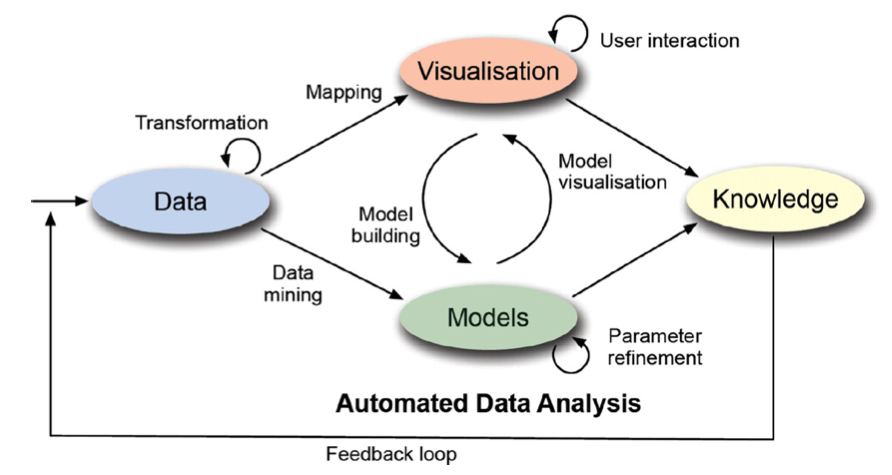
\includegraphics[width=0.5\textwidth]{images/grundlagen-visual_analytics_process.png} 
   \caption{Visual Analytics Process nach \cite{Kohlhammer2011}}
   \label{figure:visual_analytics_process}
\end{figure}

Van Wijk \cite{vanWijk2005} stellt ein ähnliches Modell für den Prozess der Wissensaufnahme über Visualisierungen vor (Abbildung~\ref{figure:visualization_model}). Am Anfang stehen die Daten $D$, welche anhand einer Visualisierungsspezifikation $S$ in eine Visualisierung $V$ transformiert werden. Diese wird vom Benutzer aufgenommen ($P$) und in Wissen ($K$) umgesetzt. Danach startet die Exploration der Daten $E$ indem die Spezifikation geändert und neues Wissen aufgenommen wird (entspricht der \enquote{Feedback loop} aus \cite{Kohlhammer2011}).

\begin{figure}[htbp]
   \centering
   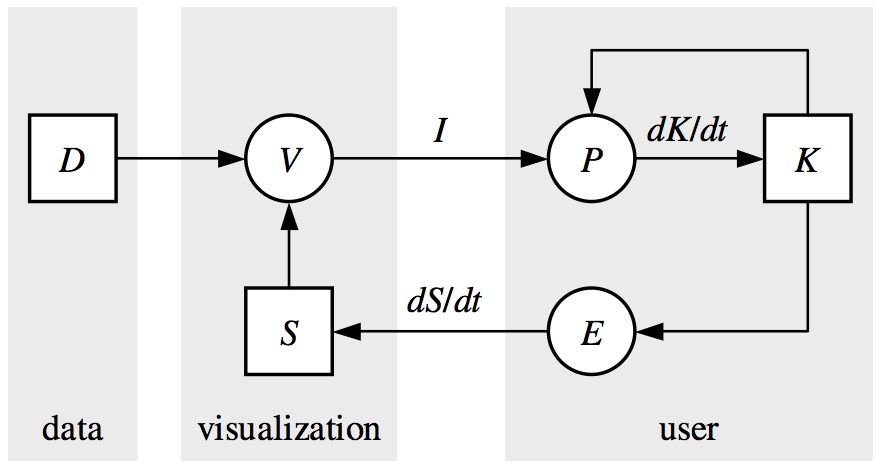
\includegraphics[width=0.5\textwidth]{images/grundlagen-visualization_model.png} 
   \caption{Generic Model on Visualization nach \cite{vanWijk2005}}
   \label{figure:visualization_model}
\end{figure}

% überblick über infovis

Im Folgenden wird ein Überblick über verschiedene Informationsvisualisierungen gegeben. Dieser orientiert sich an Keim \cite{Keim2002}, welcher Informationsvisualisierungen nach dargestellten Daten, Visualisierungs- und Interaktionstechnik klassifizierte. Die Abbildungen stammen, sofern nicht anders angegeben, aus \cite{Heer2010}.

\subsubsection{Dargestellte Daten}
\label{section:standderforschung:grundlagen:informationsvisualisierung:dargestellte_daten}

\textbf{Eindimensionale Daten} sind beispielsweise Zeitreihen, also Folgen von Daten (1992, 1993, 1995...). Nach Keim können diese aber mit anderen Datenobjekten assoziiert sein. Beispiele für InfoVis eindimensionaler Daten wären demnach ein Index Chart (Abbildung~\ref{figure:index_chart}) oder eine einfache Timeline.

\begin{figure}[htbp]
   \centering
   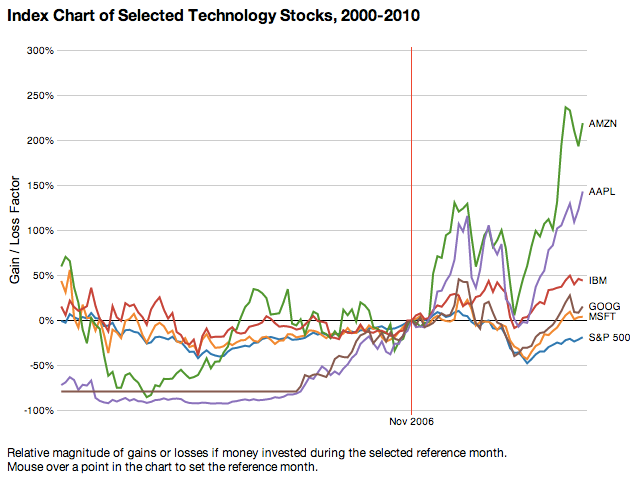
\includegraphics[width=0.5\textwidth]{images/grundlagen-index_chart.png}
   \caption{Index Chart}
   \label{figure:index_chart}
\end{figure}

\textbf{Zweidimensionale Daten} haben zwei unterschiedliche Dimensionen, wie zum Beispiel eine Geokoordinate (geografische Länge und Breite). Beispiele für InfoVis dieser Daten sind eben Karten (Abbildung~\ref{figure:karte}) oder häufig verwendete zweidimensionale Visualisierungen wie z.\,B. ein Balkendiagramm.

\begin{figure}[htbp]
   \centering
   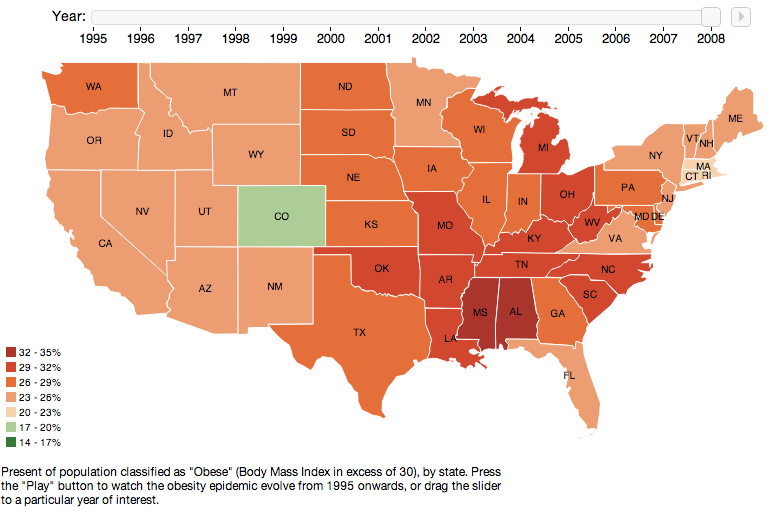
\includegraphics[width=0.5\textwidth]{images/grundlagen-karte.png}
   \caption{Karte}
   \label{figure:karte}
\end{figure}

\textbf{Multidimensionale Daten} haben demnach mehr als zwei unterschiedliche Dimensionen, typischerweise komplexe Objekte wie Autos (Hubraum, Maximalgeschwindigkeit, Leistung, Benzinverbrauch...) oder Digitalkameras (Megapixel, Sensorgröße, maximale Lichtempfindlichkeit, Gewicht...). Um diese Daten darzustellen, werden oft Parallel Coordinates (Abbildung~\ref{figure:parallel_coordinates}) oder Scatterplot Matrizen (Abbildung~\ref{figure:scatterplot_matrix}) verwendet.

\begin{figure}[htbp]
   \centering
   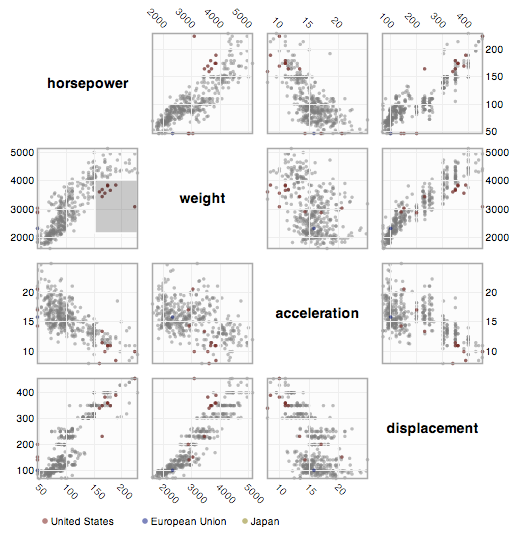
\includegraphics[width=0.5\textwidth]{images/grundlagen-scatterplot_matrix.png}
   \caption{Scatterplot Matrix}
   \label{figure:scatterplot_matrix}
\end{figure}

\textbf{Text} kann erst nach einer Vorverarbeitungsphase mit Zahlen beschrieben werden (z.\,B. Wörter zählen), ansonsten schlagen herkömmliche Visualisierungsansätze fehl. Ein im Web verbreitetes Beispiel ist die Tag Cloud (Abbildung~\ref{figure:tag_cloud}\footnote{\url{http://4.bp.blogspot.com/-WvicpJ9QqQs/TpbqvbKhX3I/AAAAAAAADGc/3PczLY2P0xs/s1600/uni_tag_cloud_wordle.png}}). Je häufiger ein Begriff im Textkorpus vorkommt, desto größer wird er dargestellt.

\begin{figure}[htbp]
   \centering
   
\includegraphics[width=0.5\textwidth]{images/grundlagen-tag_cloud.png}
   \caption{Tag Cloud}
   \label{figure:tag_cloud}
\end{figure}

\textbf{Hierarchien und Netzwerke} beschreiben Relationen und Verbindungen zwischen Objekten. Ein Beispiel für InfoVis von Hierarchien ist der klassische Baum (Abbildung~\ref{figure:baum}), für Netzwerke ein Node-Link-Diagramm (Abbildung~\ref{figure:node-link-diagramm}).

\begin{figure}[htbp]
   \centering
   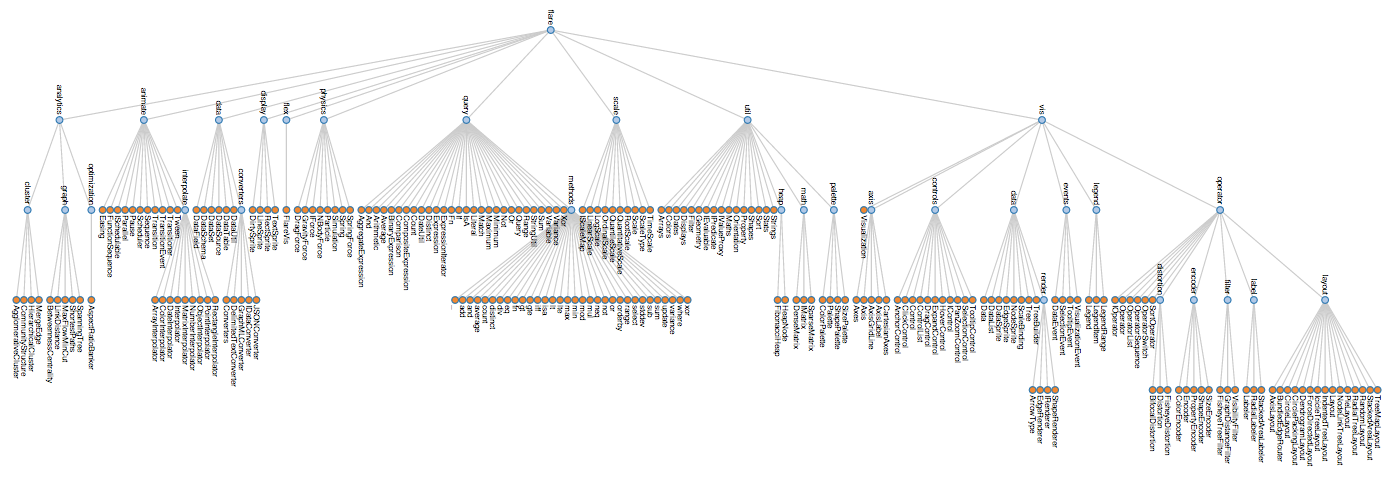
\includegraphics[width=0.75\textwidth]{images/grundlagen-baum.png}
   \caption{Baum}
   \label{figure:baum}
\end{figure}

\begin{figure}[htbp]
   \centering
   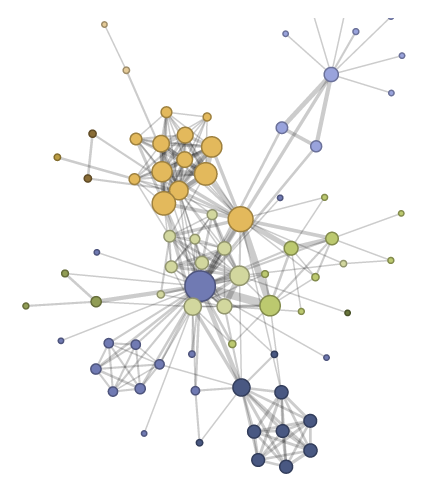
\includegraphics[width=0.25\textwidth]{images/grundlagen-node-link-diagramm.png}
   \caption{Node-Link-Diagramm}
   \label{figure:node-link-diagramm}
\end{figure}

% Am Schluss hat Keim noch Software/Algorithmen, aber ich sehe den Unterschied zu Multidimensionalen Daten nicht. Außerdem kann man - wenn schon mal grundlos neue Kategorien eingeführt werden - dann auch Produktionsprozesse oder what not gesondert betrachten

\subsubsection{Visualisierungstechniken}
\label{section:standderforschung:grundlagen:informationsvisualisierung:visualisierungstechniken}

% standard 2d/3d

\textbf{Standard 2D/3D} Visualisierungen beinhalten Balkendiagramme, Liniendiagramme, sowie andere zweidimensionale Plots und Karten. Ein Beispiel dafür ist das Index Chart (Abbildung~\ref{figure:index_chart}).

% multidimensional
\textbf{Multidimensionale} Visualisierungen\footnote{Die Bezeichnung stammt von Chi \cite{Chi2000} und wird verwendet, da sie logischer erscheint als Keims \enquote{geometrically transformed displays}.} sind Darstellungen multidimensionaler Datensätze jeder Art. Beispiele sind Parallel Coordinates (Abbildung~\ref{figure:parallel_coordinates}) und die Scatterplot Matrix (Abbildung~\ref{figure:scatterplot_matrix}).

% iconic displays

\textbf{Symbolische} Visualisierungen setzen auf verschiedene Art und Weise Symbole ein. Das können auf eine Karte projizierte Kuchendiagramme sein (Abbildung~\ref{figure:symbol_map}) oder Smileys, die abhängig von den Daten lächeln oder weinen \cite{Chernoff1973}.

\begin{figure}[htbp]
   \centering
   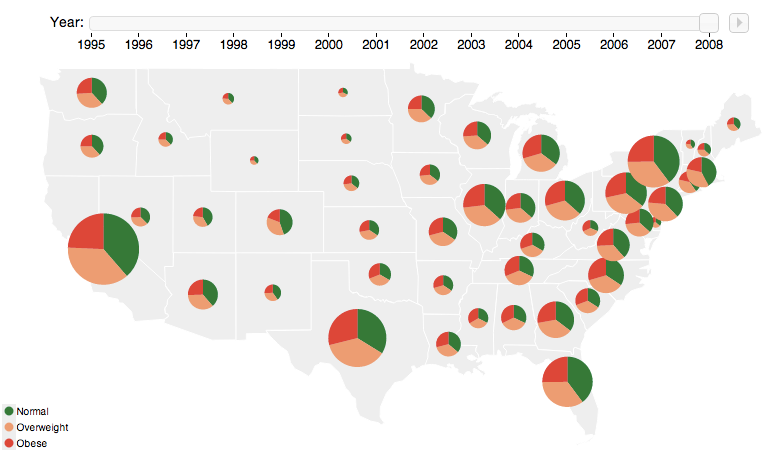
\includegraphics[width=0.5\textwidth]{images/grundlagen-symbol_map.png}
   \caption{Symbol Map}
   \label{figure:symbol_map}
\end{figure}

% dense pixel displays

\textbf{Dense Pixel} Visualisierungen assoziieren jeden Wert einer Dimension mit einem eingefärbten Pixel und platzieren die Pixel einer Dimension nebeneinander. Ein Beispiel dafür ist das Recursive Pattern \cite{Keim1995} (Abbildung~\ref{figure:recursive_pattern}).

\begin{figure}[htbp]
   \centering
   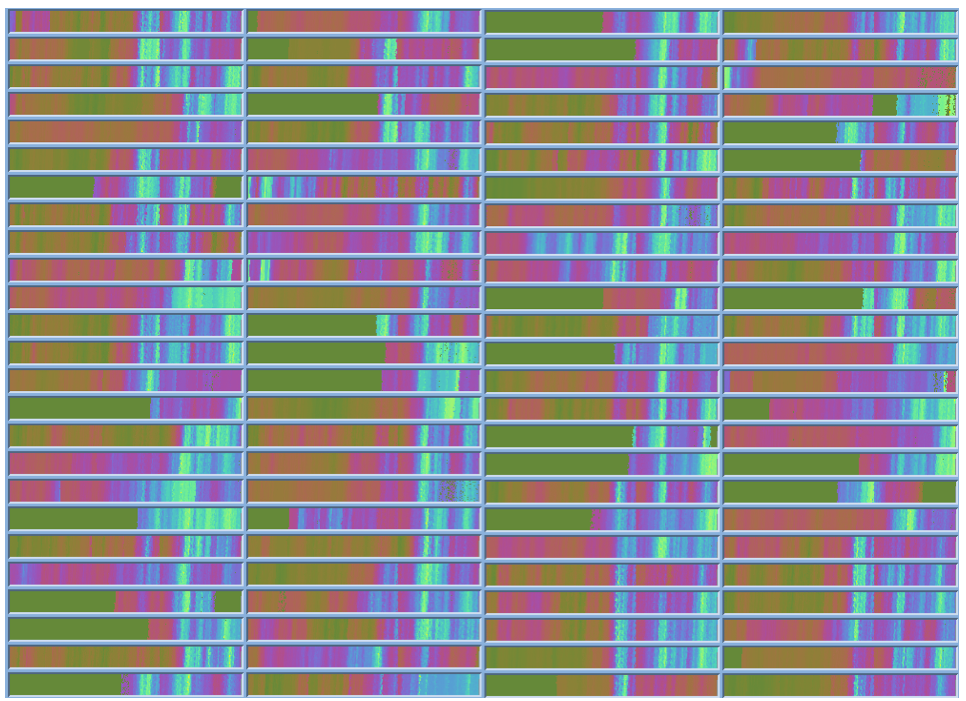
\includegraphics[width=0.5\textwidth]{images/grundlagen-recursive_pattern.png}
   \caption{Recursive Pattern}
   \label{figure:recursive_pattern}
\end{figure}

% stacked displays

\textbf{Verschachtelte} Visualisierungen repräsentieren Hierarchien, wobei Kindknoten innerhalb ihrer Eltern dargestellt werden. Beispiele dafür sind Treemaps \cite{Shneiderman1992} oder Nested Circles (Abbildung~\ref{figure:nested_circles}).

\begin{figure}[htbp]
   \centering
   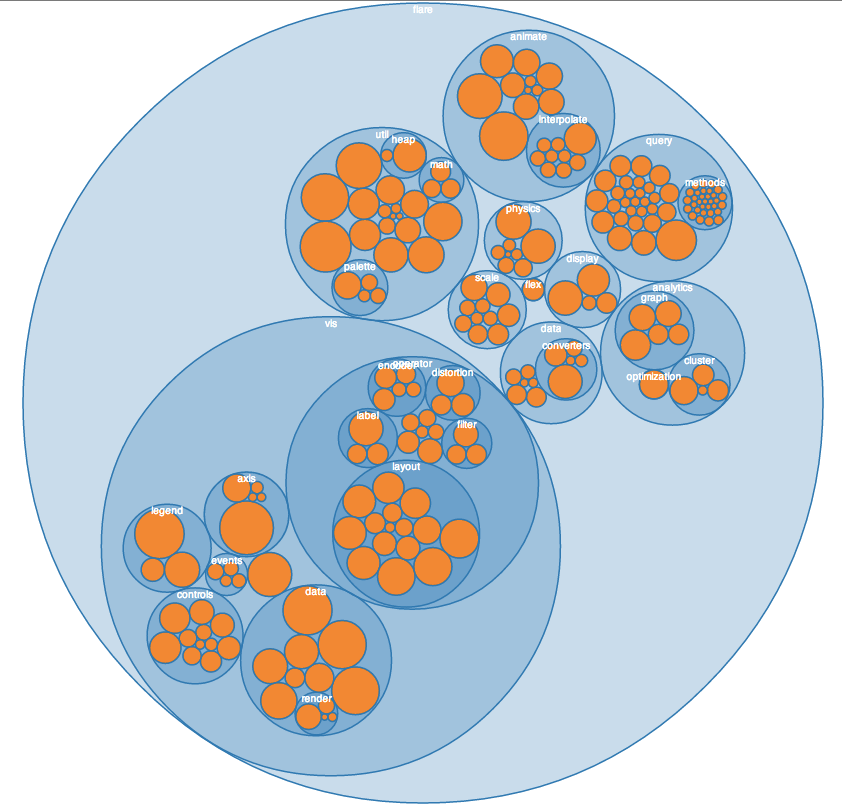
\includegraphics[width=0.25\textwidth]{images/grundlagen-nested_circles.png}
   \caption{Nested Circles}
   \label{figure:nested_circles}
\end{figure}

\subsubsection{Interaktionstechniken}
\label{section:standderforschung:grundlagen:informationsvisualisierung:interaktionstechniken}

% dynamische projektionen

\textbf{Dynamische Projektionen} zeigen dem Benutzer automatisch beispielsweise verschiedene Scatterplots des Datensatzes. Diese Interaktionstechnik eignet sich besonders für multidimensionale Datensätze. Umgesetzt wurde sie zum Beispiel in XGobi \cite{Swayne1998}.

% interaktives filtern

Durch \textbf{interaktives Filtern} bestimmt der Benutzer, welche Teilmenge des Datensatzes visualisiert wird. Das kann durch direktes Auswählen (Browsing) oder durch Bestimmen von Eigenschaften der gewünschten Daten (Querying) passieren. Letzteres ist in modernen E-Commerce-Systemen durch Facetten \cite{Yee2003} umgesetzt (Abbildung~\ref{figure:faceted_browsing}).

\begin{figure}[htbp]
   \centering
   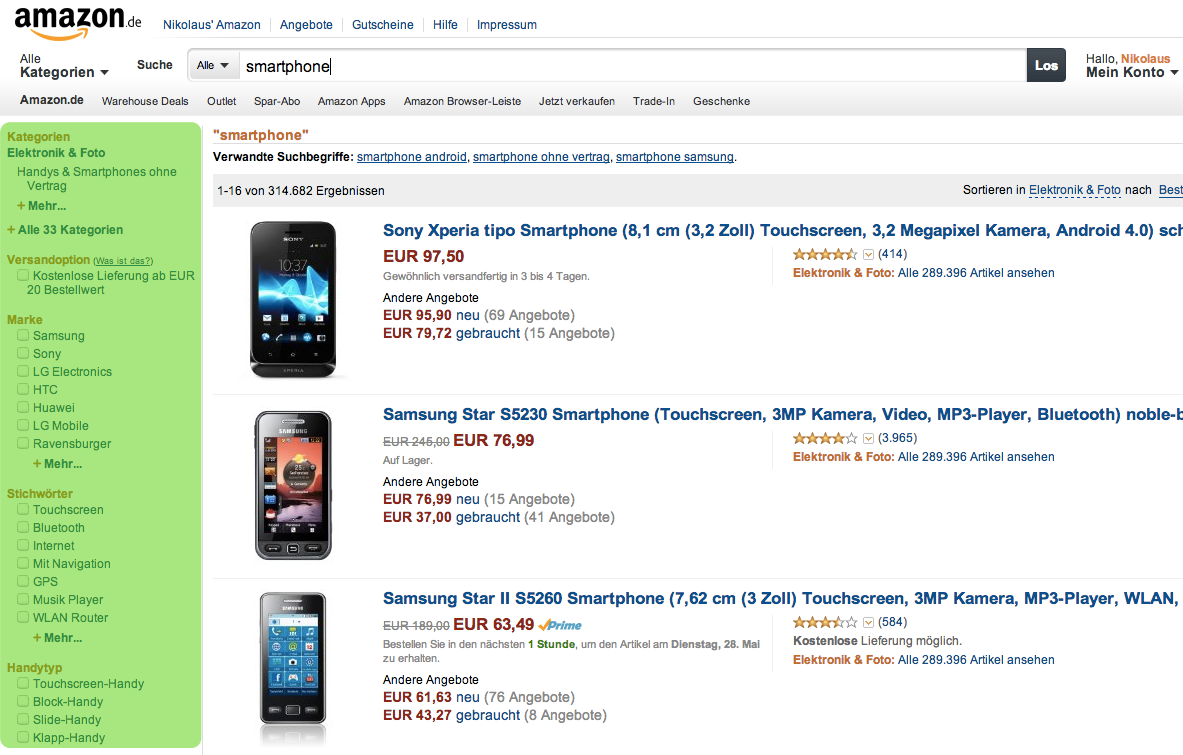
\includegraphics[width=0.5\textwidth]{images/grundlagen-faceted_browsing.png}
   \caption{Faceted Browsing bei Amazon.de}
   \label{figure:faceted_browsing}
\end{figure}

% interaktives zoomen

\textbf{Interaktives Zoomen} ermöglicht es dem Benutzer mehr oder weniger Details anzuzeigen. Damit ist nicht nur der computergrafische Vorgang der Skalierung gemeint (wie etwa bei einem Mikroskop), sondern auch schlecht sichtbare Elemente auszublenden (wie z.\,B. bei Google Maps, siehe Abbildung~\ref{figure:zoom}).

\begin{figure}[htbp]
   \centering
   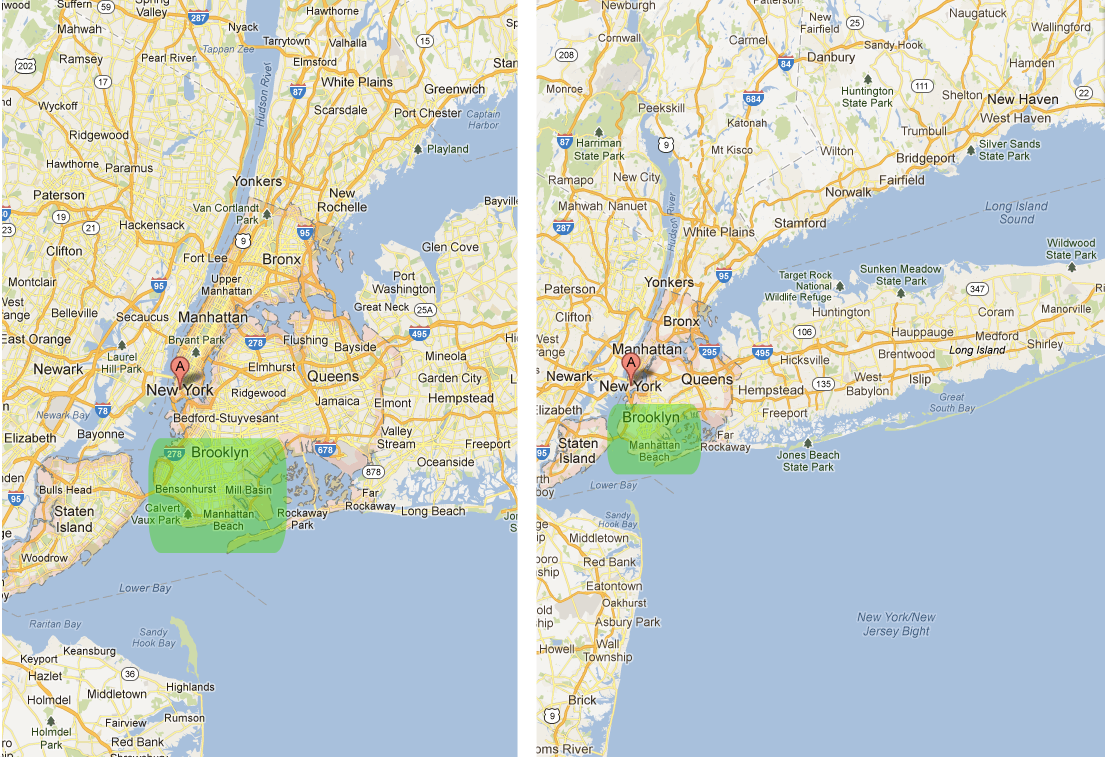
\includegraphics[width=0.5\textwidth]{images/grundlagen-zoom.png}
   \caption{Interaktiver Zoom bei Google Maps: Im rechten, ausgezoomten Bild fehlt beispielsweise die Interstate 278 (grüne Markierung)}
   \label{figure:zoom}
\end{figure}

% distortion (fisheyes and such)

Durch \textbf{Verzerrung} kann ein Bereich der Visualisierung mit hohem Detailgrad angezeigt werden, während der Rest nur wenig detailliert sichtbar ist. Ein bekanntes Beispiel dafür ist das Fisheye (Abbildung~\ref{figure:fisheye}).

\begin{figure}[htbp]
   \centering
   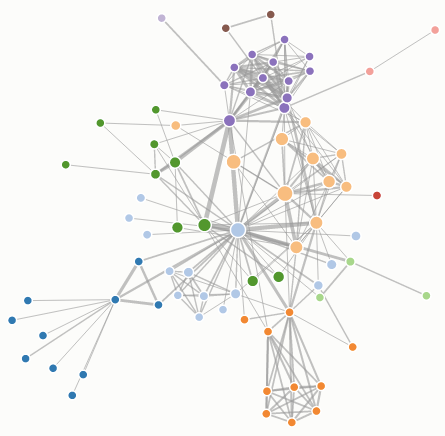
\includegraphics[width=0.5\textwidth]{images/grundlagen-fisheye.png}
   \caption{Fisheye: Das Zentrum der Verzerrung befindet sich ungefähr beim hellblauen Knoten in der Mitte}
   \label{figure:fisheye}
\end{figure}

% link & brush

\textbf{Linking \& Brushing} wird vor allem bei mehreren verschiedenen Visualisierungen eingesetzt. Die in einer Visualisierung markierten Daten werden auch in allen anderen Visualisierungen hervorgehoben. Das können zum Beispiel Scatterplots (siehe multidimensionale Visualisierungen in Abschnitt~\ref{section:standderforschung:informationsvisualisierung:visualisierungstechniken}), verschiedene Histogramme (Abbildung~\ref{figure:link_brush}\footnote{\url{http://square.github.io/crossfilter/}}) oder gemischte Visualisierungen sein.

\begin{figure}[htbp]
   \centering
   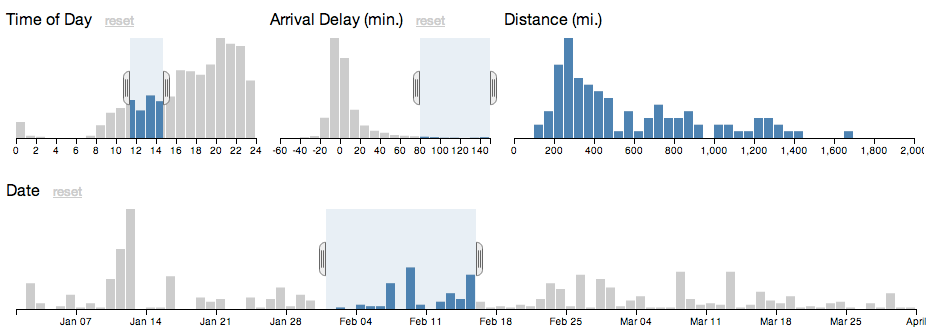
\includegraphics[width=0.75\textwidth]{images/grundlagen-link_brush.png}
   \caption{Linking \& Brushing bei Crossfilter.js: Ausgewählt wurden Flüge mit mehr als 80 Minuten Verspätung, die betroffenen Bereiche in anderen Histogrammen wurden automatisch markiert.}
   \label{figure:link_brush}
\end{figure}

todo: Was habe ich daraus jetzt gelernt?

\subsection{User Assistance}
\label{section:standderforschung:grundlagen:user_assistance}

% was ist assistance?

Der Begriff \enquote{User Assistance} steht für verschiedene Möglichkeiten, einem Benutzer zu helfen seine Ziele zu erreichen. Gapenne et al. \cite{Gapenne2002} definieren vier Beziehungstypen zwischen Mensch und Technologie, welche auch konkret auf Software übertragen werden können. Einer davon ist Assistance:

\begin{quote}
The assistance relationship appears as a sub-category of supplementation since it is not a crucial one for the actual and main activity. The function of this type of technology is to qualify and display the state and/or the becoming of the supplementation device which the subject is engaged in.
\end{quote}

Assistance sind also zum Beispiel eine Einparkhilfe im Auto oder eine Eieruhr in der Küche: Erfolgreiches Einparken oder Kochen ist auch ohne sie möglich, aber leichter mit ihnen. Supplementation hingegen erweitert die Fähigkeiten des Anwenders, also zum Beispiel eine Handprothese mit der die Pfanne angefasst werden kann.

% wie kann man assistance klassifizieren?

Rech et al. \cite{Rech2007} beschreiben intelligente Assistance in der Softwareentwicklung. Prinzipiell müssen zuerst Daten gesammelt werden, bevor die Assistance generiert und angeboten werden kann (Abbildung~\ref{figure:intelligent_assistance}). Folgende Punkte müssen in den einzelnen Schritten beachtet werden.

\begin{itemize}

	\item Daten sammeln
	\begin{itemize}
		\item Welche Datenquellen sollen benutzt werden?
		\item Wann soll die Datenanalyse stattfinden?
		\item Wie können Erkenntnisse aus den Daten gewonnen werden?
	\end{itemize}
	\item Assistance generieren
	\begin{itemize}
		\item Für wen ist die Assistance gedacht?
		\item Was soll durch Assistance erweitert werden?
		\item Für welchen Prozess/Vorgang ist die Assistance gedacht?
		\item Was ist die Zielumgebung der Assistance?
	\end{itemize}
	\item Assistance anbieten
	\begin{itemize}
		\item Wann soll Asssistance angeboten werden?
		\item Welche Modalität (visuell, akustisch usw.) soll die Assistance anbieten?
		\item Wo soll die Information angezeigt werden?
		\item Warum muss dem Benutzer geholfen werden?
	\end{itemize}
\end{itemize}

\begin{figure}[htbp]
   \centering
   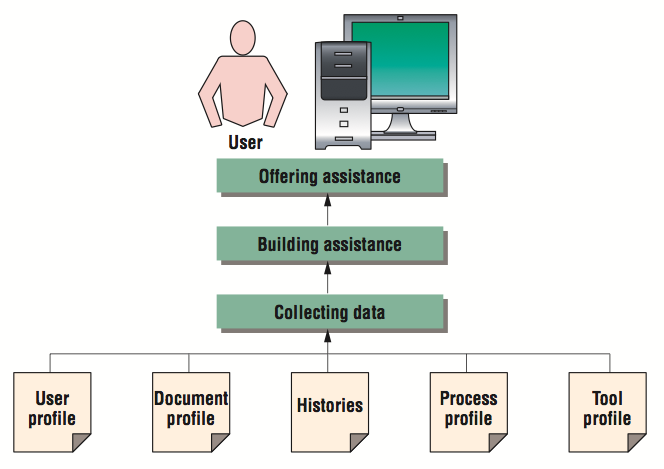
\includegraphics[width=0.5\textwidth]{images/grundlagen-intelligent_assistance.png}
   \caption{Intelligente Assistance nach \cite{Rech2007}}
   \label{figure:intelligent_assistance}
\end{figure}

Besonders die Modalität der Assistance erscheint von großer Bedeutung für eine schnelle und effektive Wissensaufnahme. Wie Information wahrgenommen wird, hat Auswirkungen sowohl auf Verständnis (\enquote{Ein Bild sagt mehr als tausend Worte}) als auch auf die benötigte Zeit. Tausend Worte können auf der Suche nach relevanten Informationen immer noch überflogen werden, eine zehnminütige akustische Hilfestellung nicht.

% effektivität von textuellen, akustischen, visuellen, gemischten erklärungen

Da kein Medium (Film, Audio, Buch etc.) besser zum Lernen geeignet ist als ein anderes \cite{Clark1994, Kozma1994} und multimodale Erklärungen effektiver als monomodale sind \cite{Mayer2002}, stellt sich die Frage, wie Multimedia-Hilfe konstruiert werden soll. Dazu kann auf die kognitive Multimedia-Lerntheorie zurückgegriffen werden. Sie geht davon aus, dass Menschen Wissen grundsätzlich über zwei Kanäle (visuell und verbal) aufnehmen, entsprechende Repräsentationen bilden und mit vorhandenem Wissen verknüpfen (Abbildung~\ref{figure:kognitive_multimedia_lerntheorie}). Die beiden Aufnahmekanäle sind in ihrer Kapazität beschränkt. Müssen zu viele Informationen verarbeitet werden, kommt es zum \enquote{Cognitive Overload} und die Lernfähigkeit wird eingeschränkt. Daraus ergeben sich vier Richtlinien zur Kontruktion der Multimedia-Erklärungen:

\begin{itemize}
	\item \textbf{Gleichzeitigkeit}: Werden akustische und visuelle Mittel eingesetzt, so sollen sie gleichzeitig präsentiert werden \cite{Mayer1991}. So können Lernende ihre visuellen und verbalen Wissensrepräsentationen besser miteinander verknüpfen.
	\item \textbf{Prägnanz}: Unterhaltsame aber irrelevante Details fördern die Erinnerungsfähigkeit an einen Text nicht \cite{Garner1989}. Deswegen sollen nur relevante Informationen vermittelt werden.
	\item \textbf{Multimodalität}: Informationen sollten möglichst auf visuelle und verbale Art vermittelt werden, um zu verhindern, dass ein Aufnahmekanal überlastet wird (bspw. durch die Darstellung einer Animation mit On-Screen-Text) \cite{Moreno1999}.
	\item \textbf{Keine Redundanz}: Aus dem selben Grund warum zweikanälige Erklärungen vorzuziehen sind, sollte auch Redundanz in einem Aufnahmekanel vermieden werden.
\end{itemize}

\begin{figure}[htbp]
   \centering
   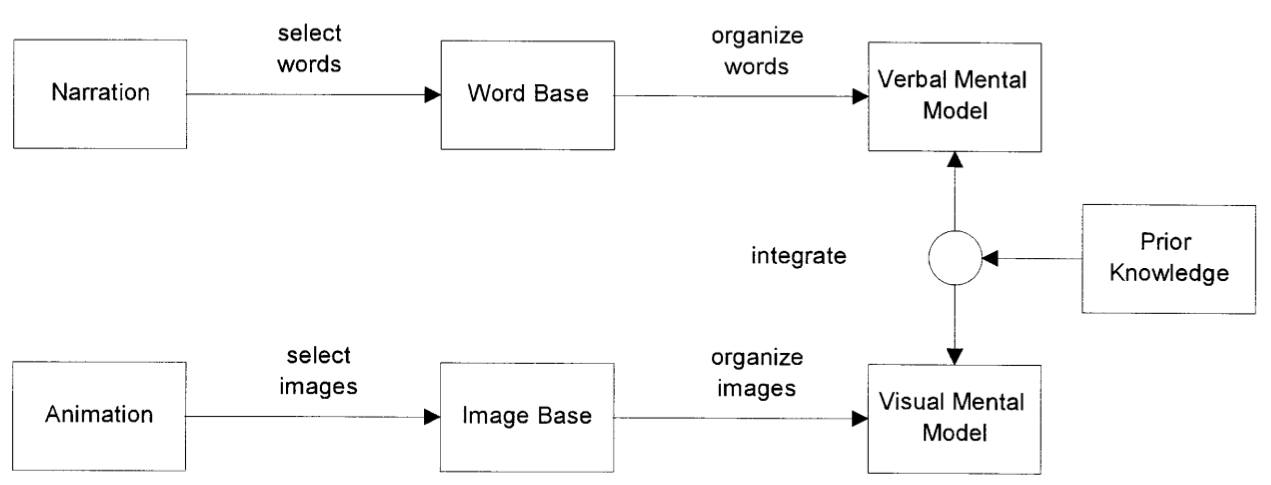
\includegraphics[width=0.75\textwidth]{images/grundlagen-kognitive_multimedia_lerntheorie.png}
   \caption{Kognitive Multimedia-Lerntheorie nach \cite{Mayer2002}}
   \label{figure:kognitive_multimedia_lerntheorie}
\end{figure}

% user assistance möglichkeiten für jede modalität

Wie kann User Assistance im visuellen bzw. verbalen Aufnahmekanal aussehen? Verbale Erklärungen können zur Laufzeit generiert werden \cite{Bauer2011, Gesell2012, Matheson2012}, sind jedoch tendenziell zu langatmig formuliert und enthalten viele Wiederholungen. Auf Grund der vorhin erwähnten Designprinzipien \enquote{Prägnanz} und \enquote{Keine Redundanz} sollte davon wahrscheinlich abgesehen und verbale Erklärungen handgeschrieben oder sehr kurz gehalten werden.

Die naheliegendste Möglichkeit für visuelle User Assistance sind Bilder. Illustrationen/Schemata sind in der Tat hilfreich, solange sowohl die Bestandteile des Systems (z.\,B. eine Luftpumpe) als auch die einzelnen Schritte des Prozesses (z.\,B. Luft einziehen, Luft auspumpen) dargestellt werden \cite{Mayer1990}. Auch Comics sind gut geeignet um Sachverhalte zu erklären (Beispiele dafür sind u.\,a. \cite{McCloud1994, McCloud2008}) und eine ansprechende Variante für User Assistance \cite{Webb2012}.

Animationen im Sinne von kurzen Videos mit abstrahiertem Inhalt können ebenfalls ein geeigneter Weg sein um Wissen zu vermitteln, sofern die erwähnten Designprinzipien eingehalten werden \cite{Mayer2002a}. Allerdings ist es möglich, dass Benutzer mit wenig Vorwissen weniger davon profitieren also solche mit viel Vorwissen \cite{Kalyuga2008}. Wenn Animationen eingesetzt werden, sollte den Benutzern Kontrolle über die Geschwindigkeit der Animation gegeben und wichtige Teile gekennzeichnet werden \cite{Wong2011}. Bei Web User Interfaces besteht die Möglichkeit konkrete Elemente der InfoVis für die Animation heranzuziehen. Das würde dem Prinzip der \enquote{Semantic Transparency} \cite{Kohlhase2009} entsprechen, wonach Benutzer möglichst direkt auf den für ihre Ziele relevanten UI-Elementen arbeiten sollen.

Filme? Hier gibt es eine Doktorarbeit, aber die finde ich online nicht \url{http://search.proquest.com/docview/1286857518}. Ansonsten scheint sich damit niemand so richtig zu beschäftigen und eigentlich ist es mir auch wurscht weil Tutorialvideos einen immer so aus dem Arbeitskontext reissen. Ich könnte es mit einer Quelle ausschließen, wenn ich die wieder finden würde... Da steht sinngemäß drin, dass Hilfe gut ist, wenn man fix wieder in den Arbeitskontext zurückkommt.


\subsubsection{Sensemaking}
\label{section:standderforschung:grundlagen:user_assistance:sensemaking}

% was ist der unterschied zwischen learning und sensemaking?
Im vorhergehenden Abschnitt wurde der Prozess der Wissensvermittlung betrachtet. Um Wissen dauerhaft aufzunehmen, müssen Lernende den Inhalt \emph{verstehen}. Der Begriff \enquote{Understanding} (gleichbedeutend mit Sensemaking) wird angewandt, wenn das Gehirn mehr Elemente des Inhalts (z.\,B. Variablen einer Gleichung) verarbeiten muss als ins Arbeitsgedächtnis passen \cite{Sweller1998}. \emph{Verstanden} hat der Lernende dann, wenn diese Elemente zu einem sogenannten Schema (mentales Modell) verarbeitet wurden und als ein einziges Element im Arbeitsgedächtnis gehalten werden können (z\,B. eine komplexe Zahl statt drei Variablen $a$, $b$ und $i$).

% wie funktioniert der prozess der wissensaneignung?

Klein \cite{Klein2006a} beschreibt in seinem Data/Frame-Modell (Abbildung~\ref{figure:data_frame_model}), wie dieser Prozess funktioniert. \enquote{Data} beschreibt dabei die Elemente des Inhalts und \enquote{Frame} das mentale Modell oder Schema. Ähnlich dem Visual Analytics Process (Abschnitt~\ref{section:standderforschung:informationsvisualisierung}) ist Sensemaking ein iterativer Prozess, aber ohne wirklichen Anfang oder Ende. Der Lernende startet mit einem Frame, versucht die Daten einzupassen und nimmt Anpassungen vor bzw. verwirft ein Frame, wenn es nicht weiter durch Daten gestützt wird. Dabei sollte der Lernende möglichst selbstständig einer Lösung kommen, nicht zu viele Daten gleichzeitig sehen und während des Prozesses keine Hypothesen aufstellen müssen, die nicht überprüft werden können \cite{Klein2006}.

\begin{figure}[htbp]
   \centering
   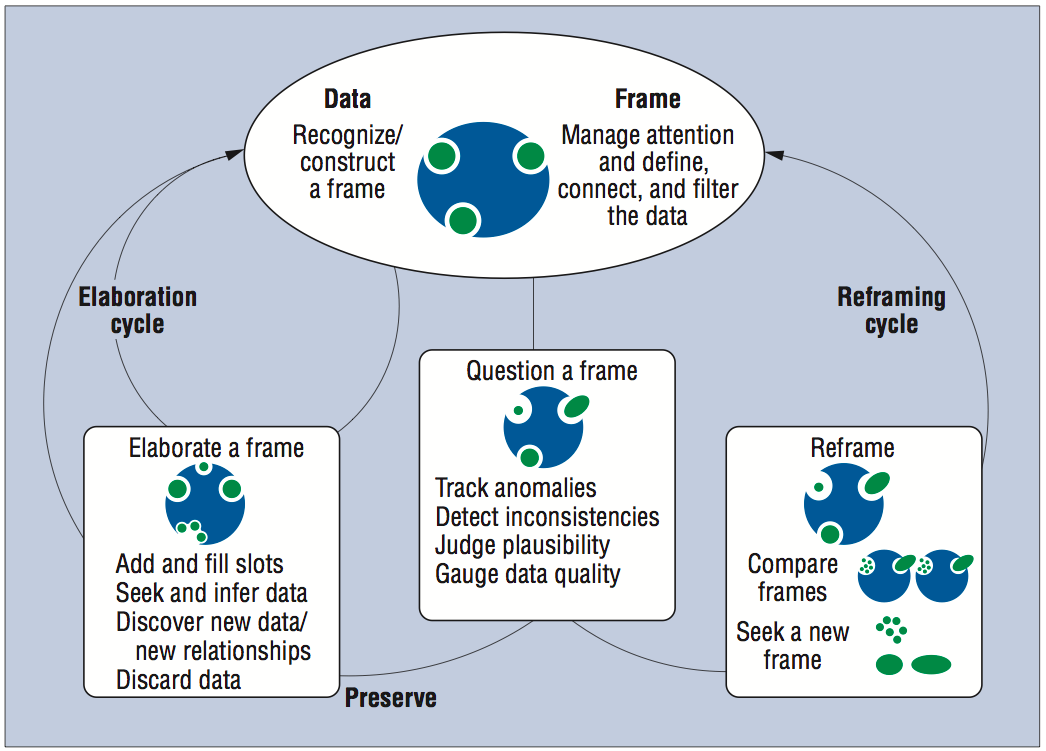
\includegraphics[width=0.75\textwidth]{images/grundlagen-data_frame_model.png}
   \caption{Data/Frame Modell nach \cite{Klein2006}}
   \label{figure:data_frame_model}
\end{figure}

% was ist dabei zu beachten?

Während des Verständnisprozesses ist es außerdem hilfreich, Wissen in irgendeiner Form externalisieren zu können, beispielsweise mit Hilfe einer Mind Map \cite{Qu2005, Novak2007, Umapathy2010}. Andere Menschen können dadurch auf bereits durchgeführte Verständnisprozesse anderer aufbauen, wobei die Struktur aber wichtiger ist als der tatsächliche Inhalt \cite{Fisher2012}.

Nachdem betrachtet wurde, wie Verständnis funktioniert, stellt sich die Frage, \emph{was} vermittelt werden soll um Menschen mit wenig InfoVis-Erfahrung zu helfen. Dazu gehört laut Grammel \cite[S. 127]{Grammel2012} unter anderem das mentale Modell des Benutzers zu verwenden, beispielsweise indem dieselben Bezeichnungen verwendet werden, und zu lehren, wie Visualisierungen verwendet und interpretiert werden.  Liu und Stasko \cite{Liu2010} schlagen folgende Definition für ein mentales Modell im Bereich der Informationsvisualisierung vor, wobei vor allem der erste Punkt über Struktur und Verhalten für ein Hilfesystem wichtig erscheint:

\begin{quote}
A mental model is a functional analogue representation to an external interactive visualization system with the following characteristics:
	\begin{itemize}
		\item The structural and behavioral properties of external systems are preserved in mental models.
		\item A mental model can preserve schematic, semantic or item-specific information about the underlying data.
		\item Given a problem, a mental model of an interactive visualization can be constructed and simulated in working memory for reasoning.
	\end{itemize}
\end{quote}

\section{Verwandte Arbeiten}
\label{section:standderforschung:verwandte_arbeiten}

Im Folgenden werden verwandte Arbeiten behandelt. Zuerst befasst sich Abschnitt~\ref{section:standderforschung:verwandte_arbeiten:mashups} mit Mashup Plattformen. Darauf folgen Visualisierungstools und Teilaspekte davon, die das Sensemaking der Nutzer verbessern sollen. Danach werden verwandte Arbeiten zu User Assistance Konzepten in Mashups und im Allgemeinen vorgestellt und zuletzt eine Zusammenfassung gegeben.

\subsection{Webbasierte Mashup Plattformen}
\label{section:standderforschung:verwandte_arbeiten:mashups}

In diesem Abschnitt werden Mashup Plattformen vorgestellt, mit denen Endnutzer Datenquellen oder UI Komponenten kombinieren können.

% yahoo pipes kombiniert nur datenquellen
% gut: intro und kommunikation
% schlecht: es können kaputte kompositionen erstellt werden (iso norm aussagekräftige fehlermeldungen)

Yahoo Pipes\footnote{\url{http://pipes.yahoo.com/pipes/}} ist eine Mashup Plattform von Yahoo, bei dem der Benutzer verschiedene Webservices mit Hilfe von Operatoren kombiniert, indem er sie interaktiv verdrahtet.
Pipes erfüllt die funktionale Anforderung \emph{Intro}, da zwei Tutorialvideos angeboten werden und eine kurze Beschreibung zu jedem Element inklusive Link zu einem Beispiel und mehr Informationen vorhanden ist. Die \emph{Kommunikation} ist durch die Drähte sichtbar, allerdings ist die Richtung des Datenflusses nicht sofort eindeutig. Pipes erleichtert die \emph{Bedienung} indem während der Drag \& Drop Operation mögliche Anknüpfungspunkte für Drähte blau eingefärbt werden.
Allerdings erschwert es die Bedienung gleichermaßen, da kaputte Kompositionen erstellt werden können und Pipes keine aussagekräftigen Fehlermeldungen ausgibt.
Für die Arbeit mit VizBoard ist es ebenfalls wichtig, die Kommunikation zwischen Komponenten nachvollziehen zu können. Da bei VizBoard der Datenfluss in beide Richtungen fließen kann, sollte darauf geachtet werden, dessen Richtung klar ersichtlich ist.

% dashmash kombiniert ui elemente und datenquellen
% gut: nutzerstudie
% schlecht: 

DashMash \cite{Cappiello2011} ist eine Mashup Plattform, die besonders auf Endnutzer ausgerichtet ist. Dazu setzt es auf das \enquote{What You See Is What You Get} Prinzip und abstrahiert von Mashup-Interna wie dem Binding zwischen Datenquellen und Komponenten. Es ist nicht möglich Erkenntnisse aus den Daten mit anderen zu teilen oder selbst Anmerkungen anderer zu lesen. Obwohl keine sichtbaren\footnote{Ein Demo-Video ist unter \url{http://home.dei.polimi.it/cappiell/demo/DemoDashMash.mov} verfügbar.} Hilfestellungen bezüglich \emph{Intro}, \emph{Bedienung} oder \emph{Kommunikation} verfügbar sind, fiel die Nutzerstudie mit 35~Teilnehmern durchweg positiv aus. Der Grund dafür ist wahrscheinlich, dass die Erklärungen am Anfang der Studie so gewählt wurden, dass die Testpersonen ein \enquote{korrektes} mentales Modell von DashMash hatten. Für die Hilfe in VizBoard sollte deswegen auch soweit möglich Technisches abstrahiert oder vor dem Benutzer versteckt werden. Des weiteren sollten Erklärungen dem mentalen Modell des Benutzers entsprechen.

% omelette auch (weil datenquellen in komponenten drin)
% gut: einfache interaktion (widget hinzufügen und das wars
% schlecht: hilfestellungen hauptsächlich für erstellung als nutzung

Apache Rave\footnote{\url{http://rave.apache.org/}} ist eine Mashup Plattform von Apache und Grundlage für OMELETTE \cite{Chudnovskyy2012}. OMELETTE stellt dem Benutzer verschiedene Widgets zur Verfügung, die er kombinieren kann. Zum Beispiel ein Widget zur Visualisierung des Wasserpegels und eine Karte, die Hochwassermeldungen zeigt. Im Gegensatz zu VizBoard besteht keine Einschränkung auf eine bestimmte Domäne. Es ist möglich Widgets zu kommentieren. Die \emph{Kommentare} werden aber nur im Widget Store angezeigt, da sie eher dem Feedback zum Widget als dem Verständnis des Inhalts dienen. Bezüglich der \emph{Bedienung} oder \emph{Kommunikation} bestehen keine Hilfestellungen. Ein \emph{Intro} wird im Widget Store in Form einer kurzen Beschreibung gegeben, welche der Entwickler verfasst hat. Die Hilfestellungen für den Benutzer fokussieren sich eher auf die Erstellung von Mashups als deren Nutzung \cite{Chowdhury2013}. So wird ein Pattern Recommender eingesetzt, der weitere Widgets zur Integration in die Komposotion vorschlägt sowie eine Automatic Composition Engine, die Widgets automatisch verbindet und damit Daten- und Kontrollflüsse ermöglicht.

% lessons learned

% man braucht gar nicht so viele hilfestellungen, wenn änderungen in der ui auf eigene interaktionen zurückgeführt werden können (nichts anderes heißt ein korrektes mentales modell zu haben)
% es muss klar sein, wo der datenfluss hingeht

In diesem Abschnitt wurden Mashup Plattformen vorgestellt, mit deren Hilfe Webservices oder UI Komponenten kombiniert werden können. Die wichtigste Erkenntnis war dabei, dass kaum Hilfestellungen nötig sind, wenn der Benutzer ein passendes mentales Modell der Anwendung hat. Dieses kann mit Hilfe von Erklärungen vermittelt werden. Erklärungen des Hilfesystems sollten deswegen ein konsistentes Modell der Anwendung und einheitliche Begriffe verwenden.

\subsection{Visualisierungstools}
\label{section:standderforschung:verwandte_arbeiten:visualisierungstools}

Im Folgenden werden Visualisierungstools vorgestellt. Sie bieten mindestens multiple Sichten (ähnlich wie Mashups), sind selbst Mashups (wenn nicht anders angegeben webbasiert) oder besonders populär.

% weave
% gut: ist ein mashup
% schlecht: user interface, keine hilfestellungen

Weave\footnote{\url{http://oicweave.org/}} ist eine Webapplikation, mit der Benutzer ein Mashup aus Visualisierungen erstellen können. Mögliche Datenquellen sind strukturierte Daten wie Tabellen und CSV Dateien. Benutzer können aus verschiedenen Visualisierungen wählen und diese an Daten binden. Das User Interface (Abbildung~\ref{figure:weave}) ist allerdings sehr komplex und Hilfe gibt es nur in Form einer Online-Dokumentation und einem kurzen Tutorialvideo.

\begin{figure}[htbp]
   \centering
   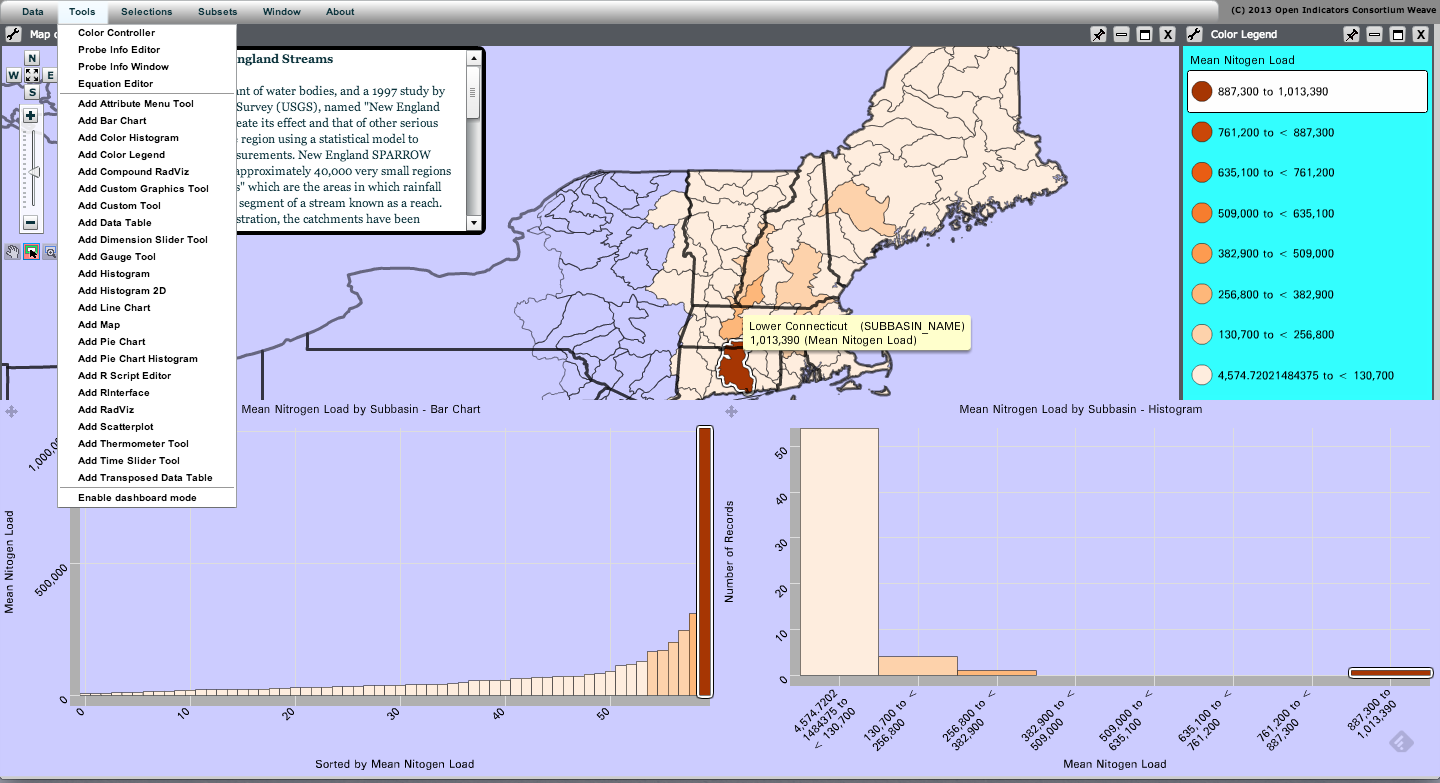
\includegraphics[width=0.75\textwidth]{images/verwandte_arbeiten-weave.png}
   \caption{Weave User Interface}
   \label{figure:weave}
\end{figure}

% polaris/tableau
% gut: interaktivität, drag & drop zeug
% schlecht: keine verlinkung

Tableau\footnote{\url{http://www.tableausoftware.com/}} ist eine Desktopapplikation, mit der aus Tabellen oder Datenbanken Diagramme erstellt werden können. Es ist der kommerzielle Nachfolger von Polaris \cite{Stolte2000} und laut Gartner \cite{Gartner2013} unter den Marktführern im Bereich Business Intelligence Platforms. Tableau setzt das Prinzip von \enquote{Semantic Transparency} um, indem der Benutzer die zu visualisierenden Daten per Drag \& Drop auf dem Diagramm platziert. Die Software muss keine umfassenden Hilfestellungen zur \emph{Bedienung} anbieten, da der Benutzer hauptsächlich Daten an das Diagramm bindet und den Diagrammtyp wechselt. Jede Aktion hat einen sofort sichtbaren Effekt, welcher mit der Undo-Funktion rückgängig gemacht werden kann. Diese drei Eigenschaften von Tableau (Semantic Transparency, Effekt sofort sichtbar, Undo/Redo) machen es sehr interaktiv, ohne dabei den Benutzer zu frustrieren. Allerdings geht Tableau davon aus, dass der Benutzer die Daten und damit verbundenen Konzepte kennt und bietet diesbezüglich keine Hilfestellungen an.

% choosel
% gut: drag n drop
% schlecht: kenntnis der daten wird vorausgesetzt

Choosel \cite{Grammel2010} ist ein Mashup, welches besonders in der Domäne Informationsvisualisierung unbedarfte Nutzer dabei unterstützen soll, Daten zu erforschen und Visualisierungen iterativ zu verfeinern. Dabei setzt es auf direkte Manipulation in Form einer erweiterten Drag \& Drop Funktion. Mögliche Drop-Ziele werden während des Vorgangs hervorgehoben und eine Vorschau des Drop-Ergebnisses wird  angeboten. Wie Tableau setzt Choosel voraus, dass der Benutzer die verwendeten Daten kennt. Im Gegensatz zu VizBoard sind bei Choosel die verfügbaren Komponenten festgelegt und stammen vom selben Entwickler. Falls im Hilfesystem für VizBoard Drag \& Drop angewendet wird, ist Choosel ein gutes Vorbild.

% mosaic
% ? ? ? 

MoSaiC \cite{Schuster2011} ist ein Tool mit dem Benutzer online kollaborativ Dokumente erstellen können. Wie bei VizBoard ist die Domäne damit festgelegt. Das Tool besteht aus verschiedenen Sichten für die Rollen der Beitragenden (Collaborators) und Organisatoren (Coordinators) und ist damit komposit, es können aber keine zusätzlichen Views aufgerufen werden. Inwieweit MoSaiC den Benutzern Hilfestellungen gibt, ist nicht bekannt, da der Autor keine Screenshots oder Videos finden konnte.

\subsubsection{Sensemaking}
\label{section:standderforschung:verwandte_arbeiten:sensemaking}

Dieser Abschnitt befasst sich mit Teilfunktionen von Visualisierungstools, die das Sensemaking der Benutzer verbessern sollen. Hauptsächlich wird dafür eine Kommentar- bzw. Annotationsfunktion eingesetzt.

% annotation
% gut: einfach zu verwenden
% schlecht: nicht geeignet wenn man keine beliebigen navigationsmöglichkeiten hat

Groth und Streefkerk \cite{Groth2006} präsentieren ein generisches Annotationssystem für Informationsvisualisierungen am Beispiel einer 3D Visualisierung von Molekülen. Grundlage des Systems sind Nutzerinteraktionen wie \enquote{rotieren}, \enquote{zoomen} etc., welche geloggt und als Graph abgespeichert werden. An den Knoten des Graphen -- Zustände der InfoVis -- können beliebig viele \emph{Kommentare} abgelegt werden. Es ist allerdings nicht möglich, innerhalb dieser Sichten noch einmal Elemente zu referenzieren (z.\,B. ein bestimmtes Atom), weswegen das System am besten für InfoVis mit uneingeschränkten Navigationsmöglichkeiten geeignet ist. Zum Beispiel einer Karte, wo mit Hilfe der Interaktionen Pan \& Zoom theoretisch ein beliebiger Punkt auf der Welt den Viewport ausfüllen kann und so eindeutig ist, worauf sich der Kommentar bezieht.

% sense.us
% gut: kommentare, diskussionen, annotationen
% schlecht: kommentare nicht an daten, kenntnis der daten wiederum vorausgesetzt

Heer et al. \cite{Heer2007} entwickelten mit sense.us einen Prototyp zur asynchronen Kollaboration mit interaktiven Visualisierungen. Benutzer können \emph{Kommentare} zu Visualisierungen hinzufügen und sie mit grafischen Annotationen (z.\,B. geometrische Formen, Pfeile, Text) versehen. Die Kommentare wurden dabei aber nicht an die Daten selbst, sondern an die Visualisierung hinzugefügt. Es war möglich, Kommentare in anderen Visualisierungen zu referenzieren. Die am meisten verwendeten Annotationstypen waren Pfeile und Text. Das alles sollte beim Entwurf der Kommentarfunktion des Hilfesystems berücksichtigt werden.

% manyeyes
% gut: kommentare
% schlecht: 

Ebenfalls erwähnenswert ist ManyEyes \cite{Viegas2007}. Benutzer können Datensätze hochladen und eine aus mehreren vorgegebenen Visualisierungen wählen. Danach können sie ähnlich wie bei sense.us die Visualisierungen \emph{kommentieren}. Wie bei sense.us können bestimmte Elemente oder Bereiche einer Visualisierung mit Kommentaren versehen werden, diese werden aber nicht visualisierungsübergreifend wiederverwendet.

% bi dashboards
% gut: annotation an daten
% schlecht: nix, eigentlich isses ziemlich geil

Elias und Bezerianos \cite{Elias2012} entwickelten ein Annotations- bzw. \emph{Kommentarsystem} für Business Intelligence Dashboards.
Dafür interviewten sie Domänenexperten und erarbeiteten sieben funktionale Anforderungen an ein annotationsgestütztes Dashboard. Dazu gehört, dass Kommentare mehrere Datenpunkte und Charts referenzieren können. Sie beschreiben außerdem ihr Handling von Annotationen und Kommentaren bei dynamischem Kontext sowie von unterschiedlichen Granularitätsstufen (Jahr/Monat/Tag). 
Diese Erkenntnisse können für VizBoard ebenfalls nützlich sein.

% infovis mit sensemaking
% gut: knowledge view
% schlecht: nur cool wenn alle inhalte fusioniert werden können. und dann ist immer noch die frage, ob man sowas wirklich braucht. bin skeptisch mit zu viel features

Shrinivasan et al. \cite{Shrinivasan2008} entwickelten ein Framework zur Informationsvisualisierung, welches den analytischen Denkprozess unterstützen soll.
Es besteht aus drei verschiedenen Views: Den InfoVis selbst, einem \enquote{Knowledge View} und einem \enquote{Navigation View}. Im Knowledge View kann der Benutzer seine Hypothesen und Analysen externalisieren, verwalten und überprüfen, sowie mit Zuständen der InfoVis verlinken. Der Navigation View erlaubt es ihm, zu einem beliebigen Punkt im Laufe der Interaktionen zurück zu gehen.
In VizBoard könnte ein Variante des Knowledge Views dazu verwendet werden eine nutzergenerierte, strukturierte Zusammenfassung eines Datensatzes zu erstellen, mit dessen Hilfe der Verständnisprozess zukünftiger Benutzer unterstützt wird. Ein Navigation View könnte zusätzlich die \emph{Bedienung} in VizBoard verbessern.

% lessons learned 

% weave: wenn UI zu komplex wird, macht es keinen spaß
% sense.us: es gibt annotationstypen, die sehr populär sind, aber nicht auf daten bezogen werden können (eben pfeile und text)
% manyeyes: keine ahnung. weder sieht es gut aus noch ist es toll zu nutzen nach heutigen standards (JAVA ALERT) noch hat es viele features.
% bi dashboards: cool wie sie das gelöst haben mit dynamischen kontext. wenn er sich ändert, wird ein snapshot vom kontext zusammen mit der annotation gespeichert. außerdem: UI für kommentare genau wie meine!!

In diesem Abschnitt wurden verschiedene Visualisierungstools und Ansätze, um das Sensemaking in ihnen zu verbessern, vorgestellt. Dabei zeigte sich am Beispiel Tableau, dass wenig Hilfestellungen nötig sind, sofern der Benutzer einfach Systemzustände als Effekt eigener Interaktionen identifizieren kann und die Anwendung einfache Rücksetzmöglichkeiten bietet. Im Fall von VizBoard ist die Situation etwas anders, da mehrere Views gleichzeitig sichtbar sind (bei Tableau ist es immer nur ein Diagramm) und der Systemzustand sich unabhängig von einer Nutzerinteraktion verändern kann (durch Komponenten, die Daten externer Webservices laden). Die Rücksetzmöglichkeit ist aber auch Teil von Shneidermans Mantra \cite{Shneiderman1996} und der ISO Norm~9241-110 \enquote{Grundsätze der Dialoggestaltung}, weswegen sie auf alle Fälle umgesetzt werden sollte.

Um den Verständnisprozess des Benutzers zu unterstützen, verwenden die meisten Systeme grafische Annotationen in Kombination mit Kommentaren. Im Fall von \cite{Elias2012} konnten die Kommentare den Benutzern helfen, neue Diagrammtypen zu verstehen. Probanden in sense.us fanden sowohl eigene als auch fremde Kommentare hilfreich. In Tableau ist es wie in \cite{Elias2012} möglich, Kommentare an Datenpunkten zu erstellen. Die Nützlichkeit von Kommentaren scheint damit außer Frage zu stehen und sie sollten auch in VizBoard implementiert werden. Dabei ist die Arbeit von Elias et al. ein guter Startpunkt, wobei aber zu beachten ist, dass die Visualisierungskomponenten bei VizBoard von fremden Entwicklern stammen und \enquote{Black Boxes} sind. Von keiner der Arbeiten aufgegriffen wurde die Möglichkeit, dass dem Benutzer Teile der Daten oder der darin verwendeten Konzepte unklar sind.

\subsection{User Assistance}

Dieser Abschnitt befasst sich mit verschiedenen Ansätzen zur User Assistance, welche die Anforderungen Verständnis, Vollständigkeit oder Unaufdringlichkeit betrifft. Dazu zählen notwendige Funktionen des Hilfesystems, mögliche Fragestellungen des Nutzers oder Interaktionskonzepte. Zunächst werden Ansätze vorgestellt, die behandeln, was dem Benutzer erklärt werden muss. Darauf folgen Konzepte zur Präsentation der Erklärung und zuletzt zur Reduktion von notwendigen Erklärungen (beispielsweise durch kluge Interaktionstechniken).

% was man erklären muss

% fragestellungen in kontextadaptiven anwendungen
% gut: welche fragen tauchen auf
% schlecht: nicht direkt für uns geeignet

Lim und Dey \cite{Lim2009} kategorisieren mögliche Fragestellungen von Nutzern in kontextadaptiven Anwendungen. Dabei ändert die Anwendung abhängig vom Nutzer- bzw. Nutzungskontext ihren Zustand (z.\,B. schaltet Smartphone auf lautlos) und der Benutzer will wissen, warum (z.\,B. weil er Abends in der Oper ist). Grundlage für Lims Ausführungen ist die Annahme, dass der Nutzer nur eingeschränkt Einfluss auf die Arbeitsweise des Systems hat, etwa durch Hinzufügen eigener Regeln. Das ist im letzten Schritt des VizBoard Workflows nicht gegeben, da der Benutzer die Visualisierungskomponenten selbst ausgewählt hat. Die Fragestellungen könnten aber hilfreich sein, wenn es um die Komponenten selbst geht (\enquote{Warum werden gerade diese Daten angezeigt?}) und so die \emph{Verständlichkeit} und \emph{Vollständigkeit} erhöhen.

% mashup debugging strategien
% gut: kam raus dass datenfluss evtl nicht so klar ist
% schlecht: 

Abgesehen von allgemeinen Fragestellungen wäre es wichtig zu wissen, ob bestimmte Mashupkonzepte besondere Beachtung finden müssen. Cao et al. \cite{Cao2010} untersuchten mit Hilfe der Thinking Aloud Methode \cite{vanSomeren1994} das Verhalten von Endnutzern, wenn sie Mashups erstellen, sowie deren Debuggingstrategien, wenn etwas nicht funktioniert. Dazu benutzten sie das inzwischen eingestellte Microsoft Popfly. In ihrer Studie hatten alle Probanden Probleme mit dem Konzept des Datenflusses, also welche Daten wann zwischen welchen Komponenten ausgetauscht werden. In VizBoard sollte überlegt werden, den Daten- bzw. Kommunikationsfluss explizit anzuzeigen und damit die \emph{Verständlichkeit} zu verbessern.

% inter widget communication
% überblick, is nix gut oder schlecht

In einem Mashup kommunizieren die beteiligten Komponenten miteinander. Weder ist dieser Vorgang für den Benutzer offensichtlich noch sollte er das Kommunikationsparadigma des Mashups lernen müssen. Chudnovskyy et al. \cite{Chudnovskyy2013} kategorisieren Probleme und Lösungsansätze, mit deren Hilfe Benutzer die Kommunikation zwischen Komponenten besser wahrnehmen können. Darunter finden sich Self-Descriptive Design, welches visuelle Hinweise und Annotationen verwendet, sowie die Surprise-Explain-Reward Strategie (Überraschung, Erklärung, Belohnung), die zeitgleich mit einem ungewöhnlichen Vorgang eine Erklärung dazu anbietet. Diese beiden Lösungsansätze könnten gut mit einer expliziten Darstellung des Kommunikationsflusses kombiniert werden.

% grammel phd & mental models
% gut: vorschläge
% schlecht: 

VizBoard ist ein Mashup von Informationsvisualisierungen, weswegen häufige Hindernisse für Endnutzer in diesem Bereich identifiziert werden müssen. Grammel \cite{Grammel2012} verfasste seine Doktorarbeit zum Thema, wie InfoVis-Anfänger Visualisierungen konstruieren. Um sie dabei zu unterstützen und ihr \emph{Verständnis} zu verbessern, schlägt er unter anderem vor, ihr mentales Modell zu verwenden (z.\,B. mit ihnen bekannten Begriffen), kontextuelle Hilfe anzubieten und es ihnen zu erleichtern, mehr über InfoVis zu lernen. Was genau ein mentales Modell bei InfoVis ausmacht, untersuchten Liu et al. \cite{Liu2010}. Demzufolge ist es besonders wichtig, die Struktur und das Verhalten der kompositen InfoVis zu erklären.

% wie man erklären kann

% textuelle erklärungen
% gut: es geht
% schlecht: sie sind langatmig

Erklärungen können nicht nur Bilder oder Videos sein, sondern auch texbasiert. Einige Arbeiten, wie z.\,B. \cite{Gesell2012, Matheson2012}, befassen sich mit der Generierung von textuellen Erklärungen. In beiden Arbeiten ist eine formale Repräsentation des Erklärungsgegenstands notwendig, beispielsweise als Baum von Vorbedingungen und \enquote{ist Teil von} Relationen oder einer Ontologie. In der Evaluation von Matheson et al. merkten einige Probanden an, dass deren Erklärungen zu langatmig seien, was gegenläufig zur Anforderung \emph{Verständlichkeit} ist.

% erklärung mit screenshots
% gut: visuell
% schlecht: nicht automatisch

Um kontextuelle Hilfe mit Bildern einfach umsetzen zu können, entwickelten Yeh et al. \cite{Yeh2011} ein Tool für Entwickler, Lehrer oder den technischen Support. Mit dieser Software sollen sie einfach Screenshots einer Anwendung erstellen und Kommentare sowie grafische Annotationen hinzufügen können. Eine Nutzerstudie wurde nicht durchgeführt, dennoch erscheint dieser Ansatz geeignet, um einfache Ursache-Wirkung Relationen zu veranschaulichen. Um in VizBoard die \emph{Einheitlichkeit} der Hilfe zu gewährleisten, müsste die Generierung aber automatisiert werden.

% user assistance mit comics
% gut: effektiv und besser als PP
% schlecht: 

Ein ähnlicher Ansatz von Hilfe mit Bildern ist der Einsatz von Comics. Webb et al. \cite{Webb2012} überprüften in einer Nutzerstudie, wie User Assistance in Form eines Comics gegenüber einer PowerPoint-Präsentation angenommen wird. Comics lagen in allen Fragestellungen (einfache Nutzung, attraktiv, nützlich, verständlich) vorne, am Besten wurden Comics angenommen, die eine Metapher beinhalteten. Da von Komponentenentwicklern nicht erwartet werden kann, einen Comic zu erstellen, müsste dieser generiert werden. Damit befassten sich unter anderem schon \cite{Kurlander1996, Shamir2006, Chan2009, Wen2012} mit unterschiedlichen Kontexten, es ist also möglich.

% kontextuelle hilfe im web

Um auf Webseiten kontextuelle Hilfe anbieten zu können, entwickelten Chilana et al. LemonAid \cite{Chilana2012}. Dabei wählen Benutzer ein beliebiges UI Element aus und bekommen dann eine Liste von Fragen und Antworten dazu angezeigt. Beispielsweise könnte ein HTML \texttt{input} Element ausgewählt werden, in das die Telefonnummer eingetragen werden muss. LemonAid erklärt, warum die Telefonnummer unverzichtbar ist, indem es auf die entsprechende FAQ Seite verweist. Da VizBoard webbasiert ist, kann dasselbe Interaktionspattern auch dort angewendet werden. Visualisierungskomponenten können UI Elemente aber dynamisch erzeugen, darauf müsste Rücksicht genommen werden.  

% wie man bedarf an erklärungen reduzieren kann

% heuristiken für infovis
% gut: undo/redo, visuelle konsistenz
% schlecht: anwendbarkeit? visuelle konsistenz haben wir ja nicht und wollen nicht.

Erklärungen zur Bedienung sind nötig, wenn der Benutzer nicht weiß, wie er eine Aktion ausführen kann (\enquote{Gulf of Execution} nach Norman \cite{Norman1986}). Der Bedarf an Erklärungen kann somit reduziert werden, wenn es die Anwendung nicht zu diesem Gulf of Execution kommen lässt. Zu diesem Zweck wurden einige Richtlinien zur User Interface Gestaltung entwickelt. Dazu gehören unter anderem die ISO9241-110, Sheidermans Mantra \cite{Shneiderman1996} oder die Heuristiken nach Nielsen \cite{Nielsen1994}. Forsell und Johansson \cite{Forsell2010} führten eine Nutzerstudie durch, um aus diesen verschiedenen Richtlinien bzw. Heuristiken zur Heuristischen Evaluation \cite{Nielsen1994} diejenigen herauszufiltern, welche bei Informationsvisualisierungen hilfreich sind. Darunter finden sich Support für Undo/Redo, visuelle Konsistenz und den mentalen Aufwand des Nutzers gering zu halten. So kann die \emph{Verständlichkeit} und \emph{Unaufdringlichkeit} des Hilfesystems von VizBoard erhöht werden.

% mashup debugging
% gut: präventiv fehler erkennen, undo
% schlecht: 

Mit Designrichtlinien im weitesten Sinne beschäftigten sich auch Kuttal et al. \cite{Kuttal2013}. Ein Nachteil von Yahoo Pipes war, dass kaputte Mashups entstehen können. Also entwickelten sie ein System zur automatischen Fehlererkennung in Yahoo Pipes, welches auch gleichzeitig die Fehlermeldungen verständlicher formulierte. In der Nutzerstudie zeigte sich, dass Benutzer mit dem System erfolgreicher Mashups erstellen konnten als ohne. Die Autoren stellen in ihrer Arbeit auch Designrichtlinien vor und raten dazu, keine technische Begriffe zu verwenden und Undo-Möglichkeiten sowie kontextuelle Hilfe anzubieten. Das deckt sich mit den Empfehlungen bisher betrachteter verwandter Arbeiten.

% grafische history für tableau
% gut: verständlich, einfach zu nutzen
% schlecht: 

Um die Undo-Funktionalität in Tableau zu verbessern entwickelten Heer et al. \cite{Heer2008} eine grafische History für Tableau. Sie zeigt Screenshots des Visualisierungszustands, die chronologisch wie eine Timeline angeordnet sind. Ein Klick auf einen Screenshot setzt die Visualisierung in den angezeigten Zustand zurück. Dieses Konzept könnte zur \emph{Verständlichkeit} von VizBoard beitragen, wenn es umsetzbar ist.

% lessons learned

% was muss erklärt werden: struktur und verhalten von infovis
% wie kann erklärt werden: kontextuelle hilfe mit bildern scheint gute möglichkeit
% wie kann weniger erklärt werden: visuelle konsistenz, undo/redo, 

In diesem Abschnitt wurden verschiedene Ansätze zur User Assistance im Allgemeinen und bei Mashups sowie InfoVis im Speziellen betrachtet. Zu der Frage, was erklärt werden muss, konnte als Antwort die Struktur und das Verhalten der Anwendung identifiziert werden, da diese Teil des mentalen Modells des Benutzers sind. Es wurde außerdem gezeigt, dass textuelle Erklärungen langatmig und deswegen visuelle Hilfestellungen besser geeignet sein können. Dazu können Screenshots oder Comics verwendet werden. Die Herausforderung bei VizBoard wäre in diesem Fall, dass sie automatisch generiert werden müssten. Um die Interaktion mit VizBoard besser zu gestalten, kann auf Designrichtlinien für Informationsvisualisierungen zurückgegriffen werden. Diese beinhalten unter anderem visuelle Konsistenz, Undo/Redo, zusätzliche Informationen anzeigen oder den mentalen Aufwand des Benutzers zu reduzieren. Bei VizBoard sind viele der Richtlinien abhängig von den Komponentenentwicklern, aber einige können auch durch das Hilfesystem umgesetzt werden.

\section{Zusammenfassung}
\label{section:standderforschung:zusammenfassung}

yay

% ###################################################
\chapter{Konzeption}
\label{chapter:konzeption}

Basierend auf dem Szenario (Abschnitt~\ref{section:standderforschung:szenario}), den Grundlagen (Abschnitt~\ref{section:standderforschung:grundlagen}) und den Erkenntnissen aus den verwandten Arbeiten (Abschnitt~\ref{section:standderforschung:verwandte_arbeiten}) wird ein Konzept zur User Assistance für das webbasierte, komposite Informationsvisualisierungssystem VizBoard erstellt. Dabei werden Hilfestellungen unterteilt in allgemeine, die jedem auf CRUISe basierenden Mashup nützlich sein können (Abschnitte~\ref{section:konzeption:intro}, \ref{section:konzeption:bedienung}, \ref{section:konzeption:feedback}, \ref{section:konzeption:kommunikation}, \ref{section:konzeption:history}, \ref{section:konzeption:meta-hilfe}) und domänenspezifische, welche besonders für Informationsvisualisierungen gedacht sind (Abschnitte~\ref{section:konzeption:verlinkung}, \ref{section:konzeption:kommentare}). Die Ziele richten sich dabei nach der Anforderungsanalyse (Abschnitt~\ref{section:standderforschung:anforderungsanalyse}).

\section{Einführung}
\label{section:konzeption:einfuehrung}

Blublublu

\subsection{Rollenmodell}
\label{section:konzeption:einfuehrung:rollenmodell}

Bei der Konzeption spielt eine große Rolle, wer für welche Tätigkeit verantwortlich ist. Um diese Fragen klären zu können, wird an dieser Stelle ein Rollenmodell für VizBoard eingeführt (Abbildung~\ref{figure:rollenmodell}).

\begin{figure}[htbp]
   \centering
   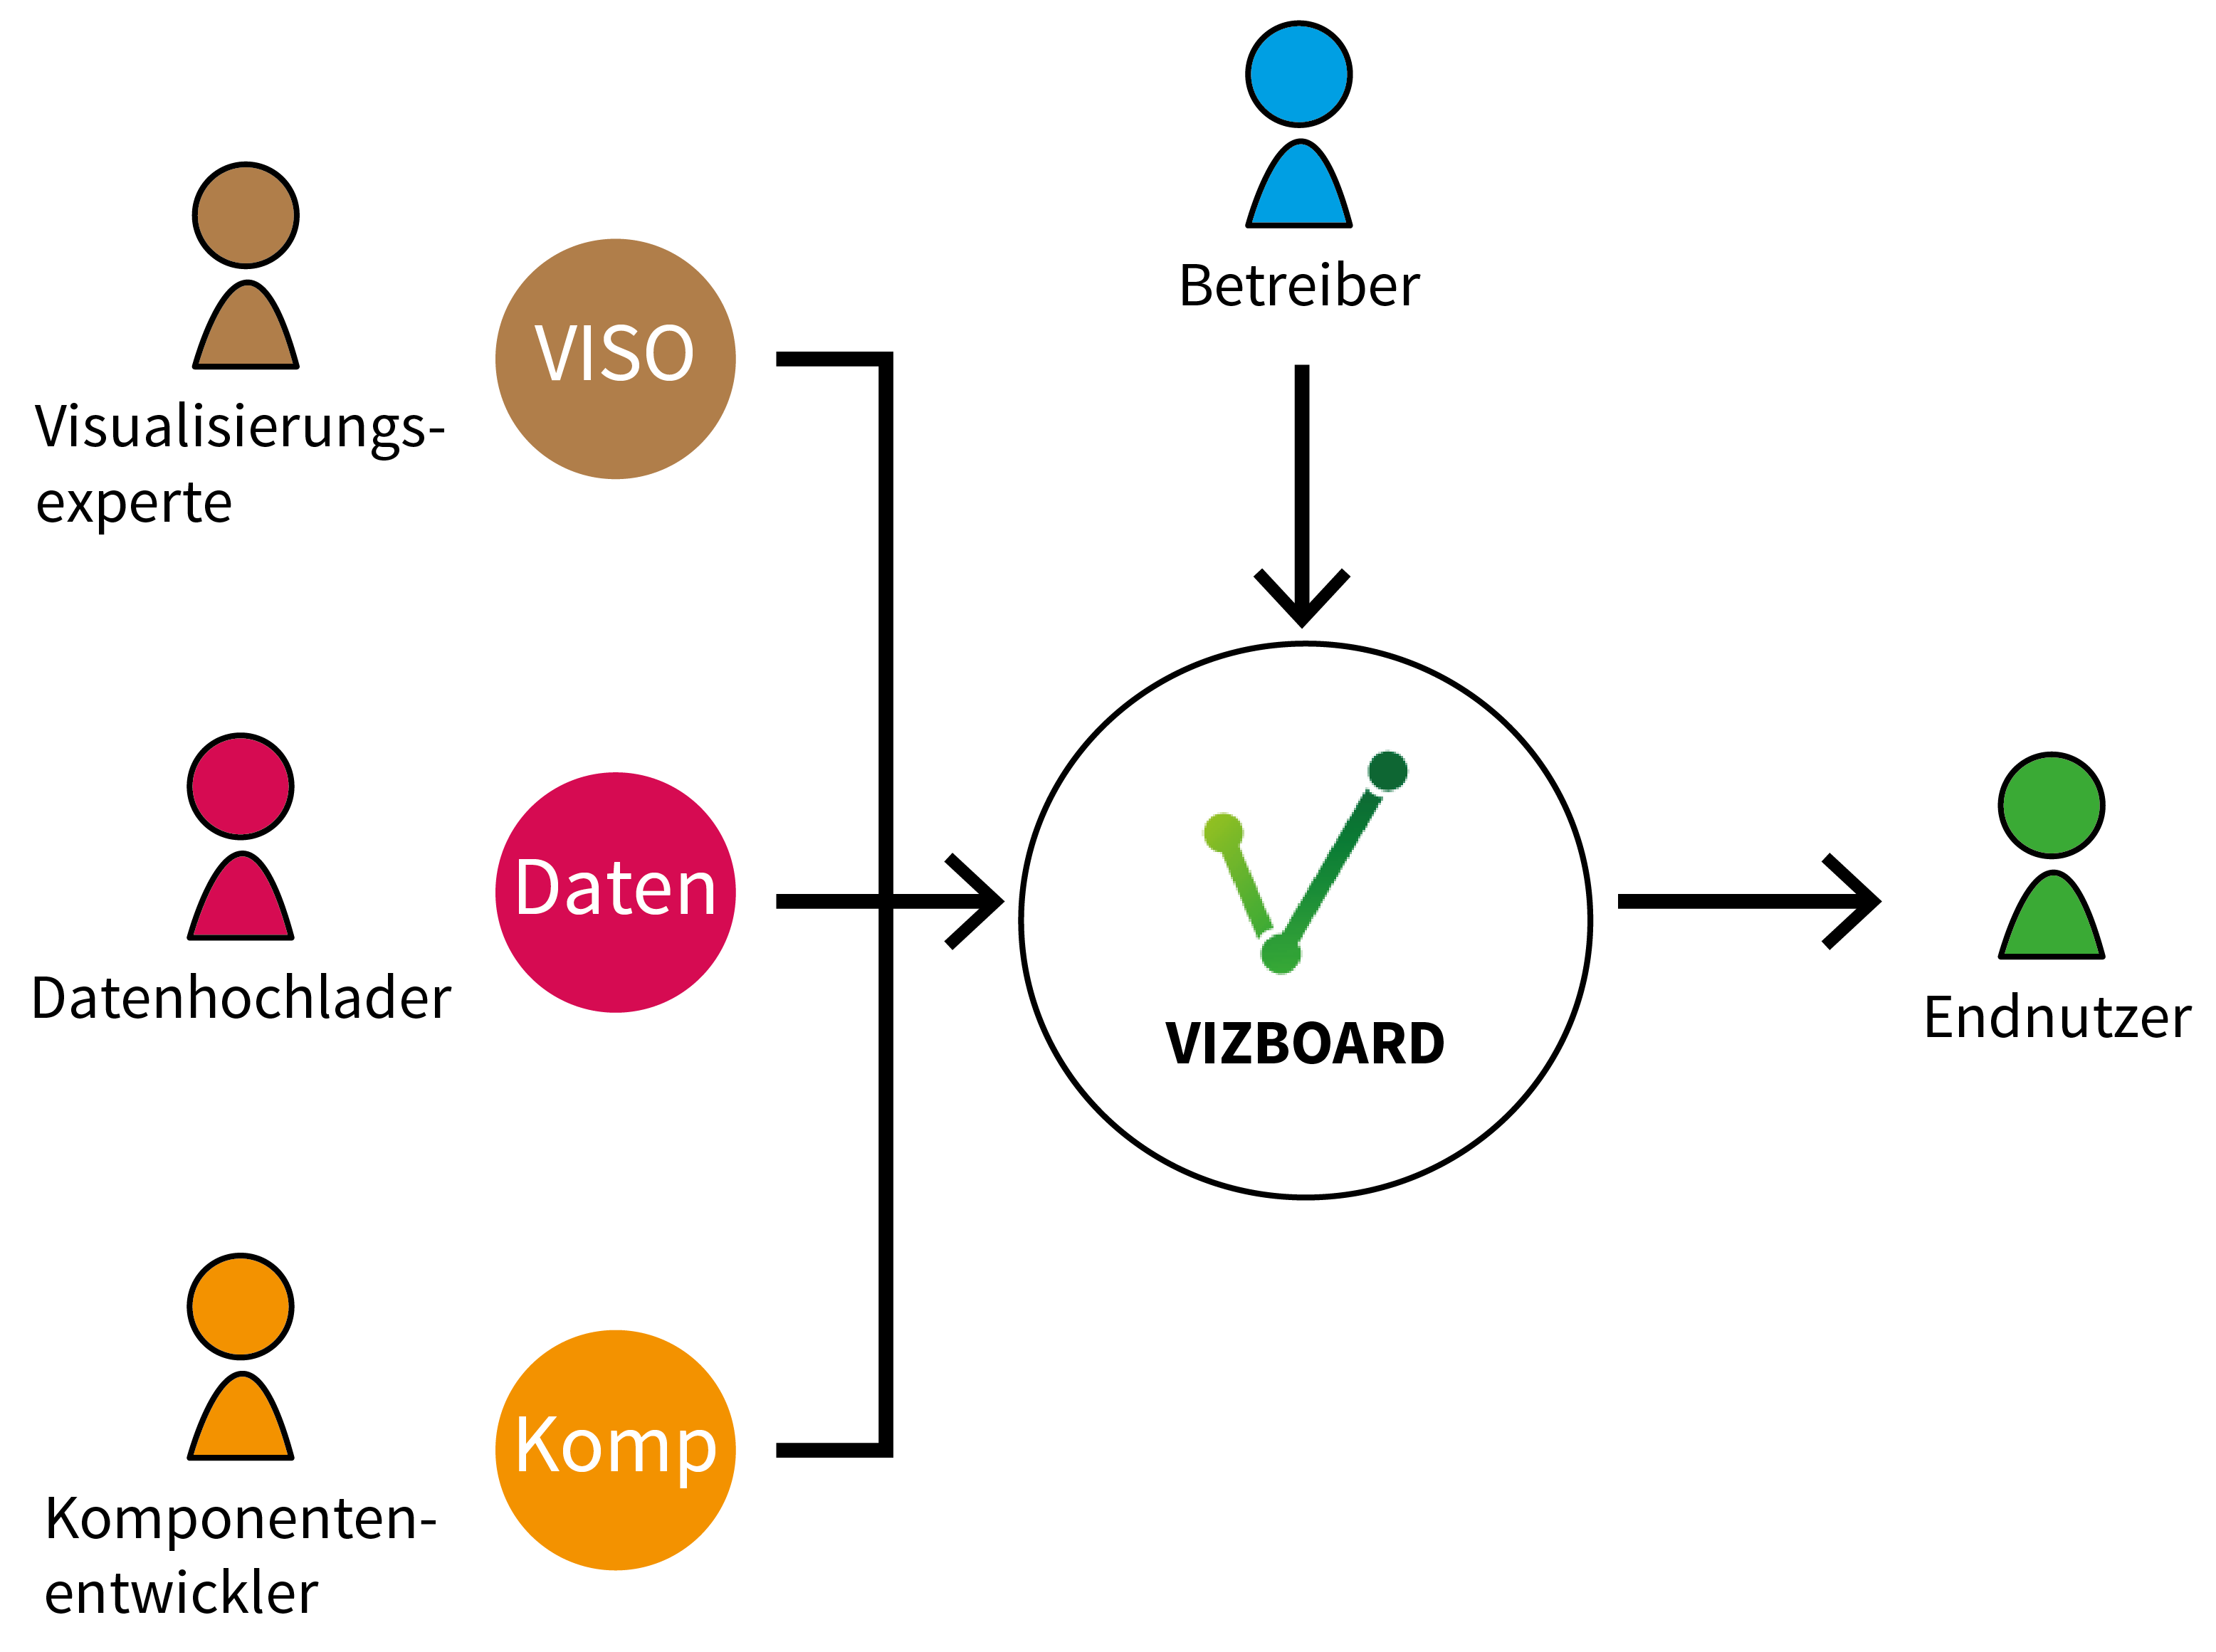
\includegraphics[width=0.5\textwidth]{images/konzeption-rollenmodell.png}
   \caption{Rollenmodell von VizBoard}
   \label{figure:rollenmodell}
\end{figure}

Das System VizBoard muss von jemandem betrieben werden. Der \textbf{Betreiber} bezahlt die Serverkosten und ist für Wartung und Instandhaltung von VizBoard verantwortlich. Für ihn ist wichtig, dass die anderen Parteien zufrieden sind, sodass sein System auch genutzt wird.

VizBoard greift auf die VISO zurück, eine Ontologie von Wissen über Informationsvisualisierung. Der \textbf{Visualisierungsexperte} besitzt Expertenwissen in der Domäne der InfoVis und formalisiert sein es in der VISO, um VizBoard zu verbessern.

Ein wichtiger Teil von VISO sind die vorhandenen Daten. Der \textbf{Datenhochlader}\todo{what} stellt Datensätze in unterschiedlichen Formaten (z\,B. APIs, RDF oder Excel Daten) zur Verfügung, die von Administratoren -- also letztlich dem Betreiber -- in VizBoard hochgeladen werden können.

Ebenso wichtig wie die Daten sind die Komponenten, die sie visualisieren. Sie werden von \textbf{Komponentenentwicklern} geschrieben und bei VizBoard registriert. Komponentenentwickler können programmieren und kennen sich teilweise auch mit InfoVis aus.

Der \textbf{Endnutzer} verwendet VizBoard, um Wissen in semantischen Datensätzen aufnehmen zu können. Er weiß weder über InfoVis noch über semantische Daten Bescheid und verfügt auch nicht über Programmierkenntnisse.

\subsection{User Interface}
\label{section:konzeption:einfuehrung:ui}

Im Laufe der Konzeption werden zum besseren Verständnis einige User Interface Mockups entworfen. Diese basieren auf der Grundlage aus dem Szenario (Abschnitt~\ref{section:standderforschung:szenario}). Die dort erwähnte Komposition enthält eine Karte, eine Treemap, eine Tabelle und ein Balkendiagramm (Abbildung~\ref{figure:ui-grundlage}). In den verwandten Arbeiten (Abschnitt~\ref{section:standderforschung:verwandte_arbeiten}) war die visuelle Konsistenz eine Designrichtlinie, welche das Bedürfnis nach Hilfestellungen verringern kann. Aus diesem Grund wird im folgenden ein Styleguide für das Hilfesystem beschrieben.

\begin{figure}[htbp]
   \centering
   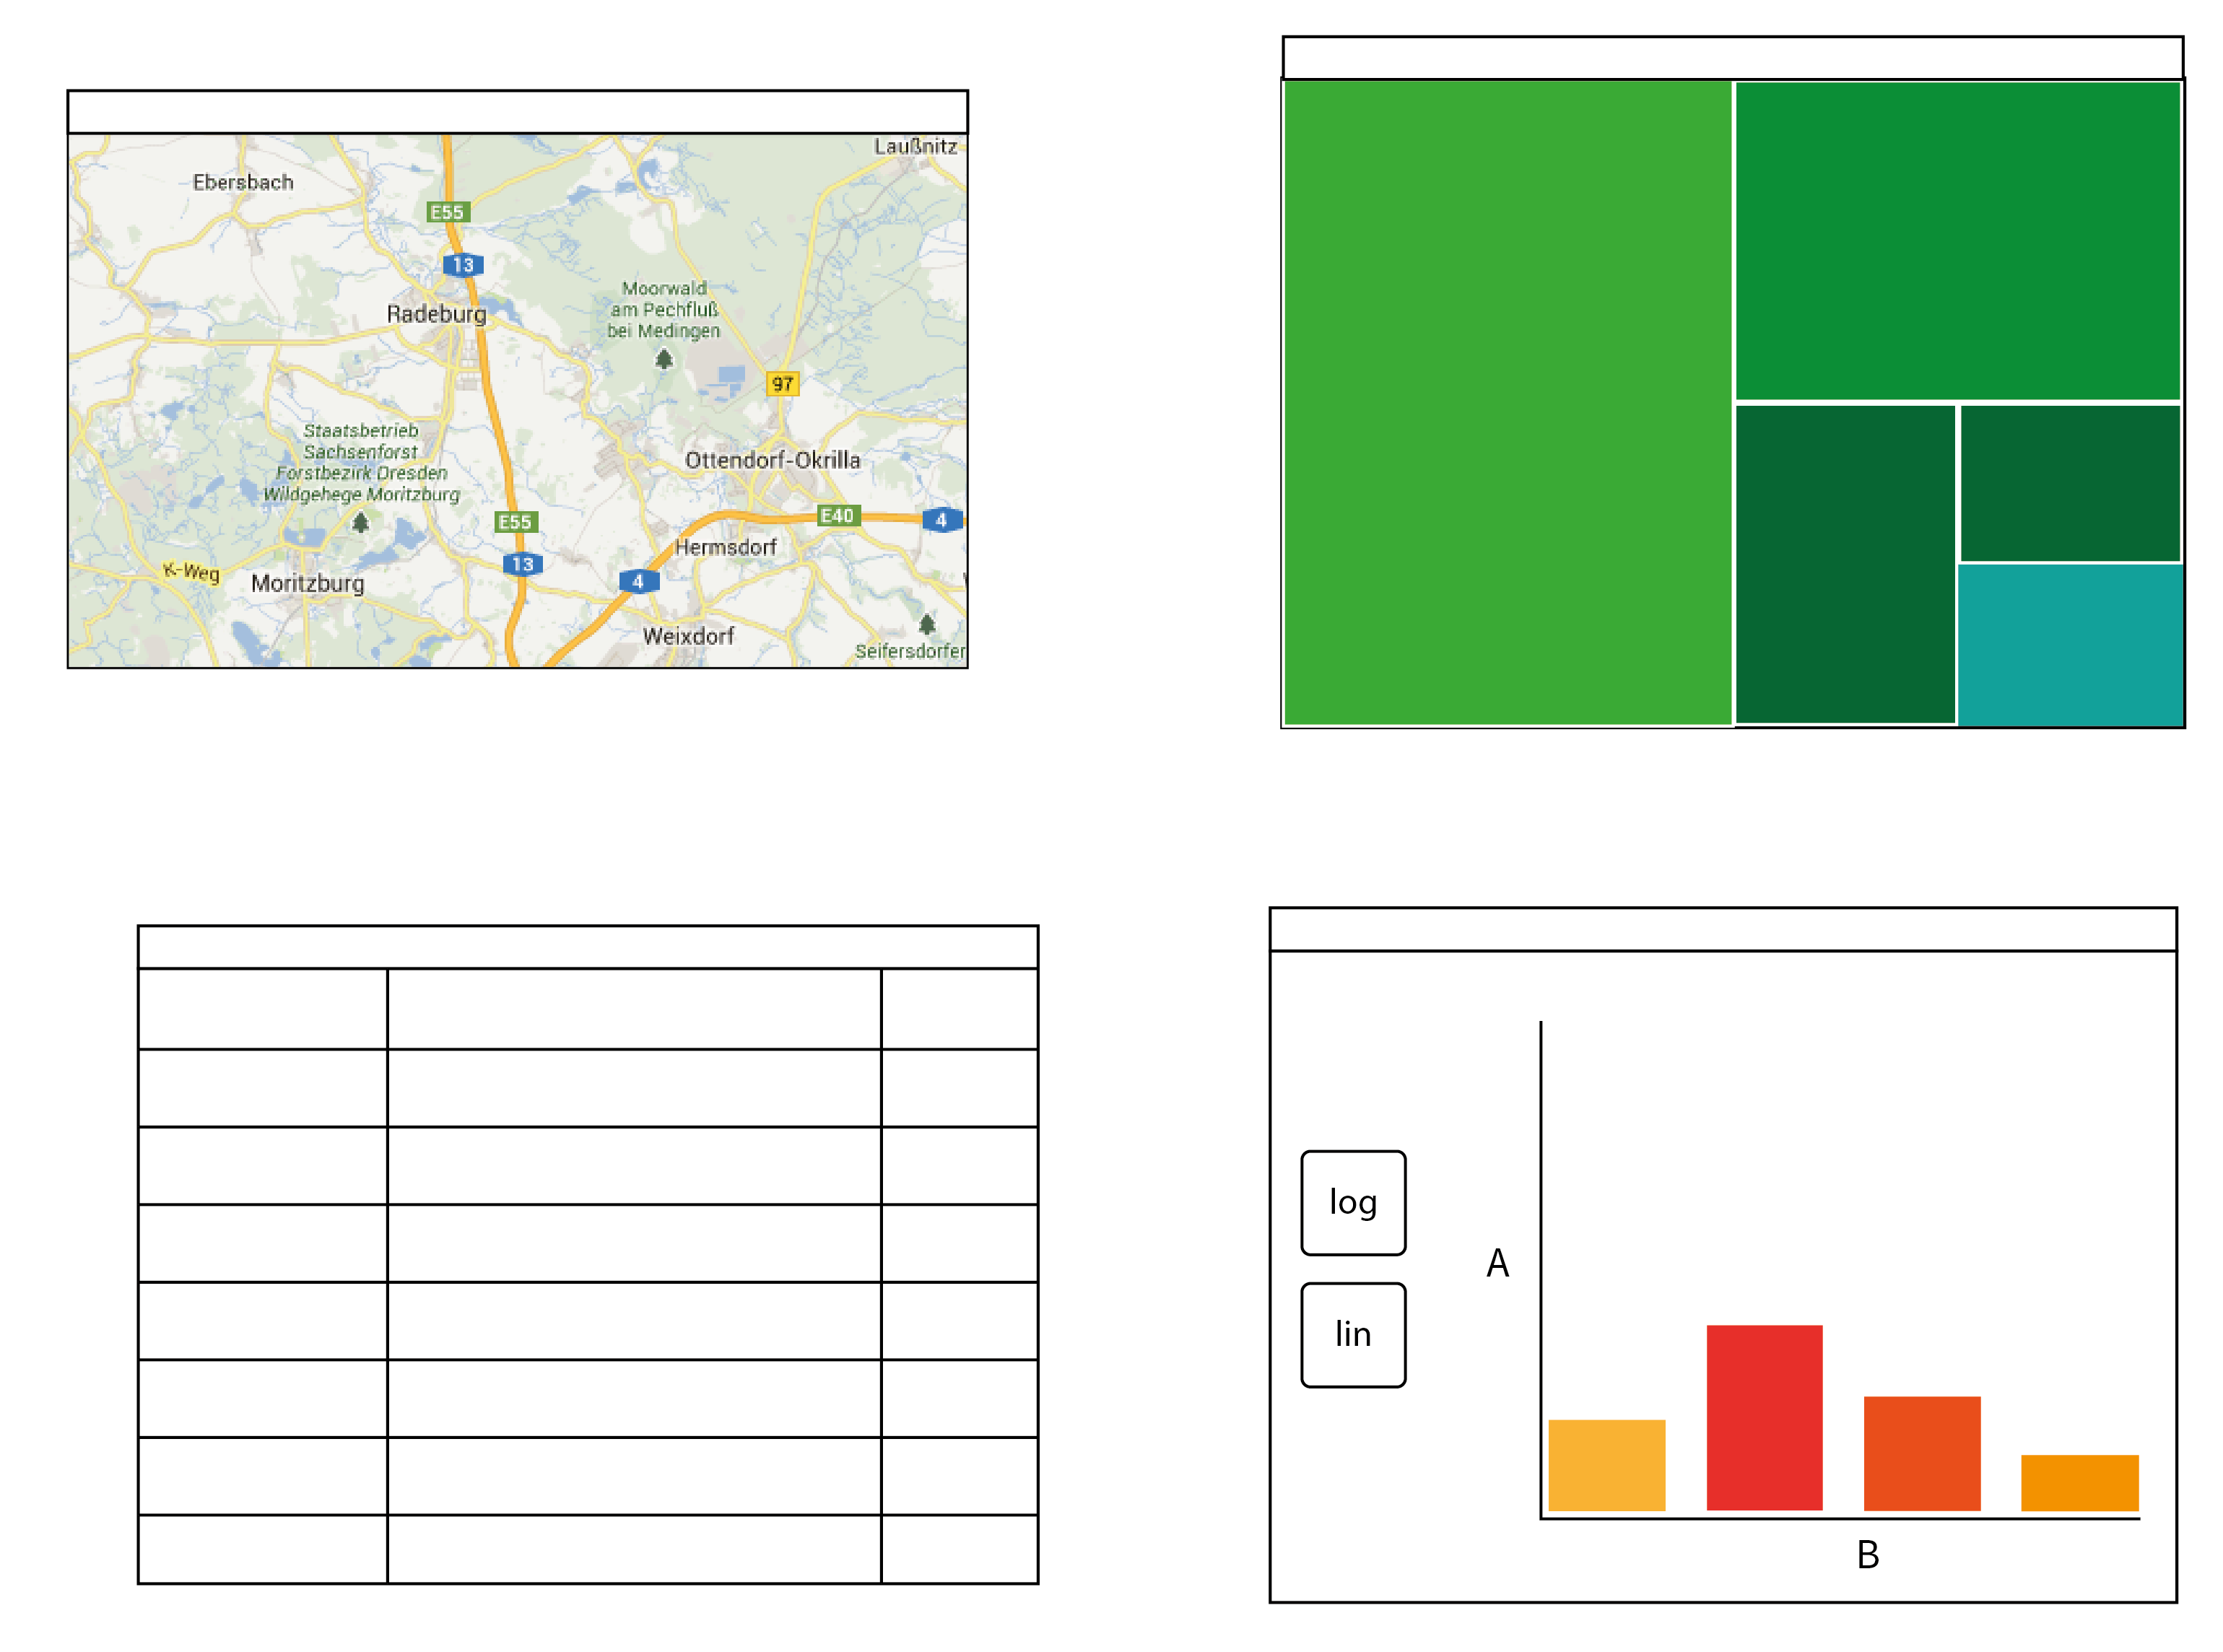
\includegraphics[width=0.5\textwidth]{images/konzeption-ui-grundlage.png}
   \caption{Grundlage der UI Mockups}
   \label{figure:ui-grundlage}
\end{figure}

\subsubsection{Art}

% wie sieht ui für dings grob aus?

Das User Interface für die ausgewählte Hilfefunktion wird links oder rechts der Komponente in einer Sidebar dargestellt (Abbildung~\ref{figure:ui-basics},~1). Gegenüber einem Popover (2) hat sie den Vorteil, dass sie sowohl links als auch rechts funktioniert. Ein Popover kann nur über der Titelleiste angezeigt werden, ansonsten werden große Teile der Komponente verdeckt (3). Die Sidebar kann in der Größe variieren (4), da für die Kommentare vermutlich mehr Platz benötigt wird als beispielsweise für die Feedbackfunktion.

\begin{figure}[htbp]
   \centering
   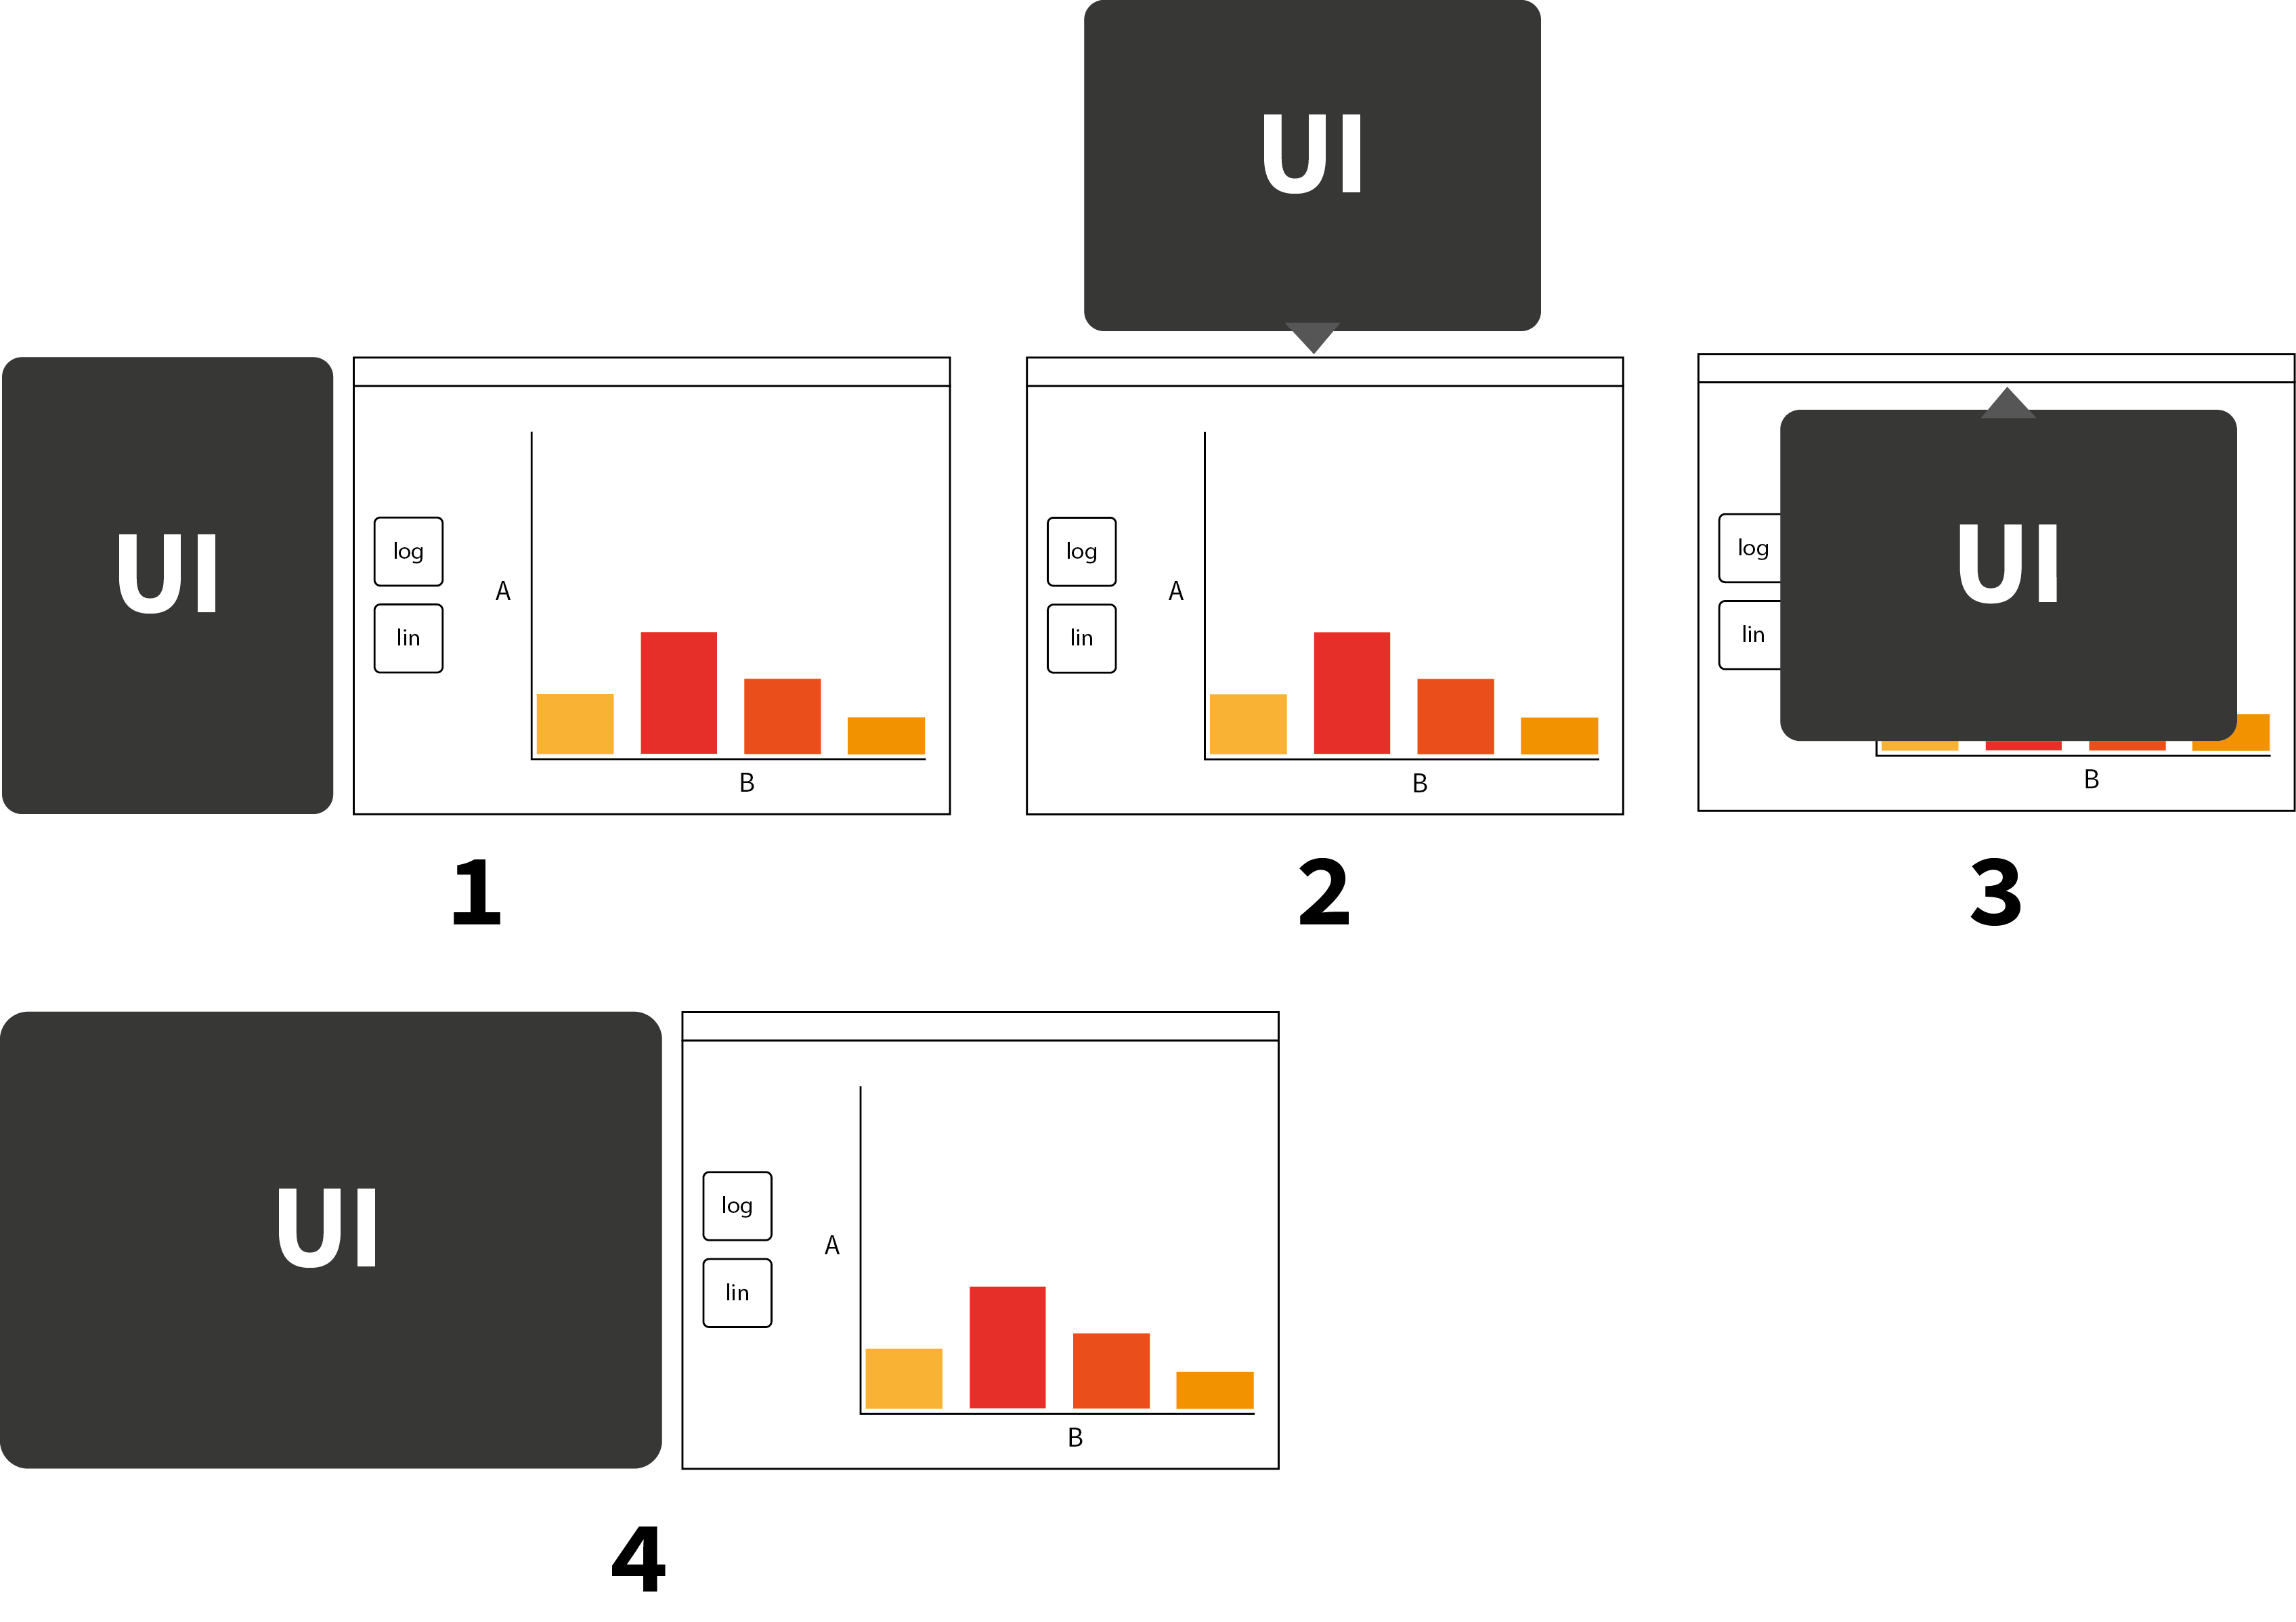
\includegraphics[width=0.5\textwidth]{images/konzeption-ui-basics.png}
   \caption{Verschiedene Möglichkeiten zur Platzierung der Hilfe UI}
   \label{figure:ui-basics}
\end{figure}

\subsubsection{Ort}

Dass die Sidebar mal links, mal rechts angezeigt wird, könnte beim Nutzer für Verwirrung sorgen. Jedoch scheint dieses Problem das kleinste zu sein, wenn man über die Alternativen nachdenkt.
Beispielsweise könnte das Hilfesystem die Buttons in einer eigenen Button-Sidebar platzieren (Abbildung~\ref{figure:ui-buttonleiste}). Allerdings erscheint dann in 50~\% der Fälle die UI Sidebar auf der anderen Seite, was noch verwirrender ist (Abbildung~\ref{figure:ui-buttonleiste}, 1 und 2). Zwar wäre es möglich, die Button-Sidebar auf beiden Seiten der Komponente anzuzeigen und eine davon zu deaktivieren (Abbildung~\ref{figure:ui-buttonleiste}, 3). Diese Variante unterscheidet sich aber nicht viel von der eben beschriebenen, da der Benutzer dann nicht die Buttons selbst, sondern aktivierte Buttons suchen muss.

\begin{figure}[htbp]
   \centering
   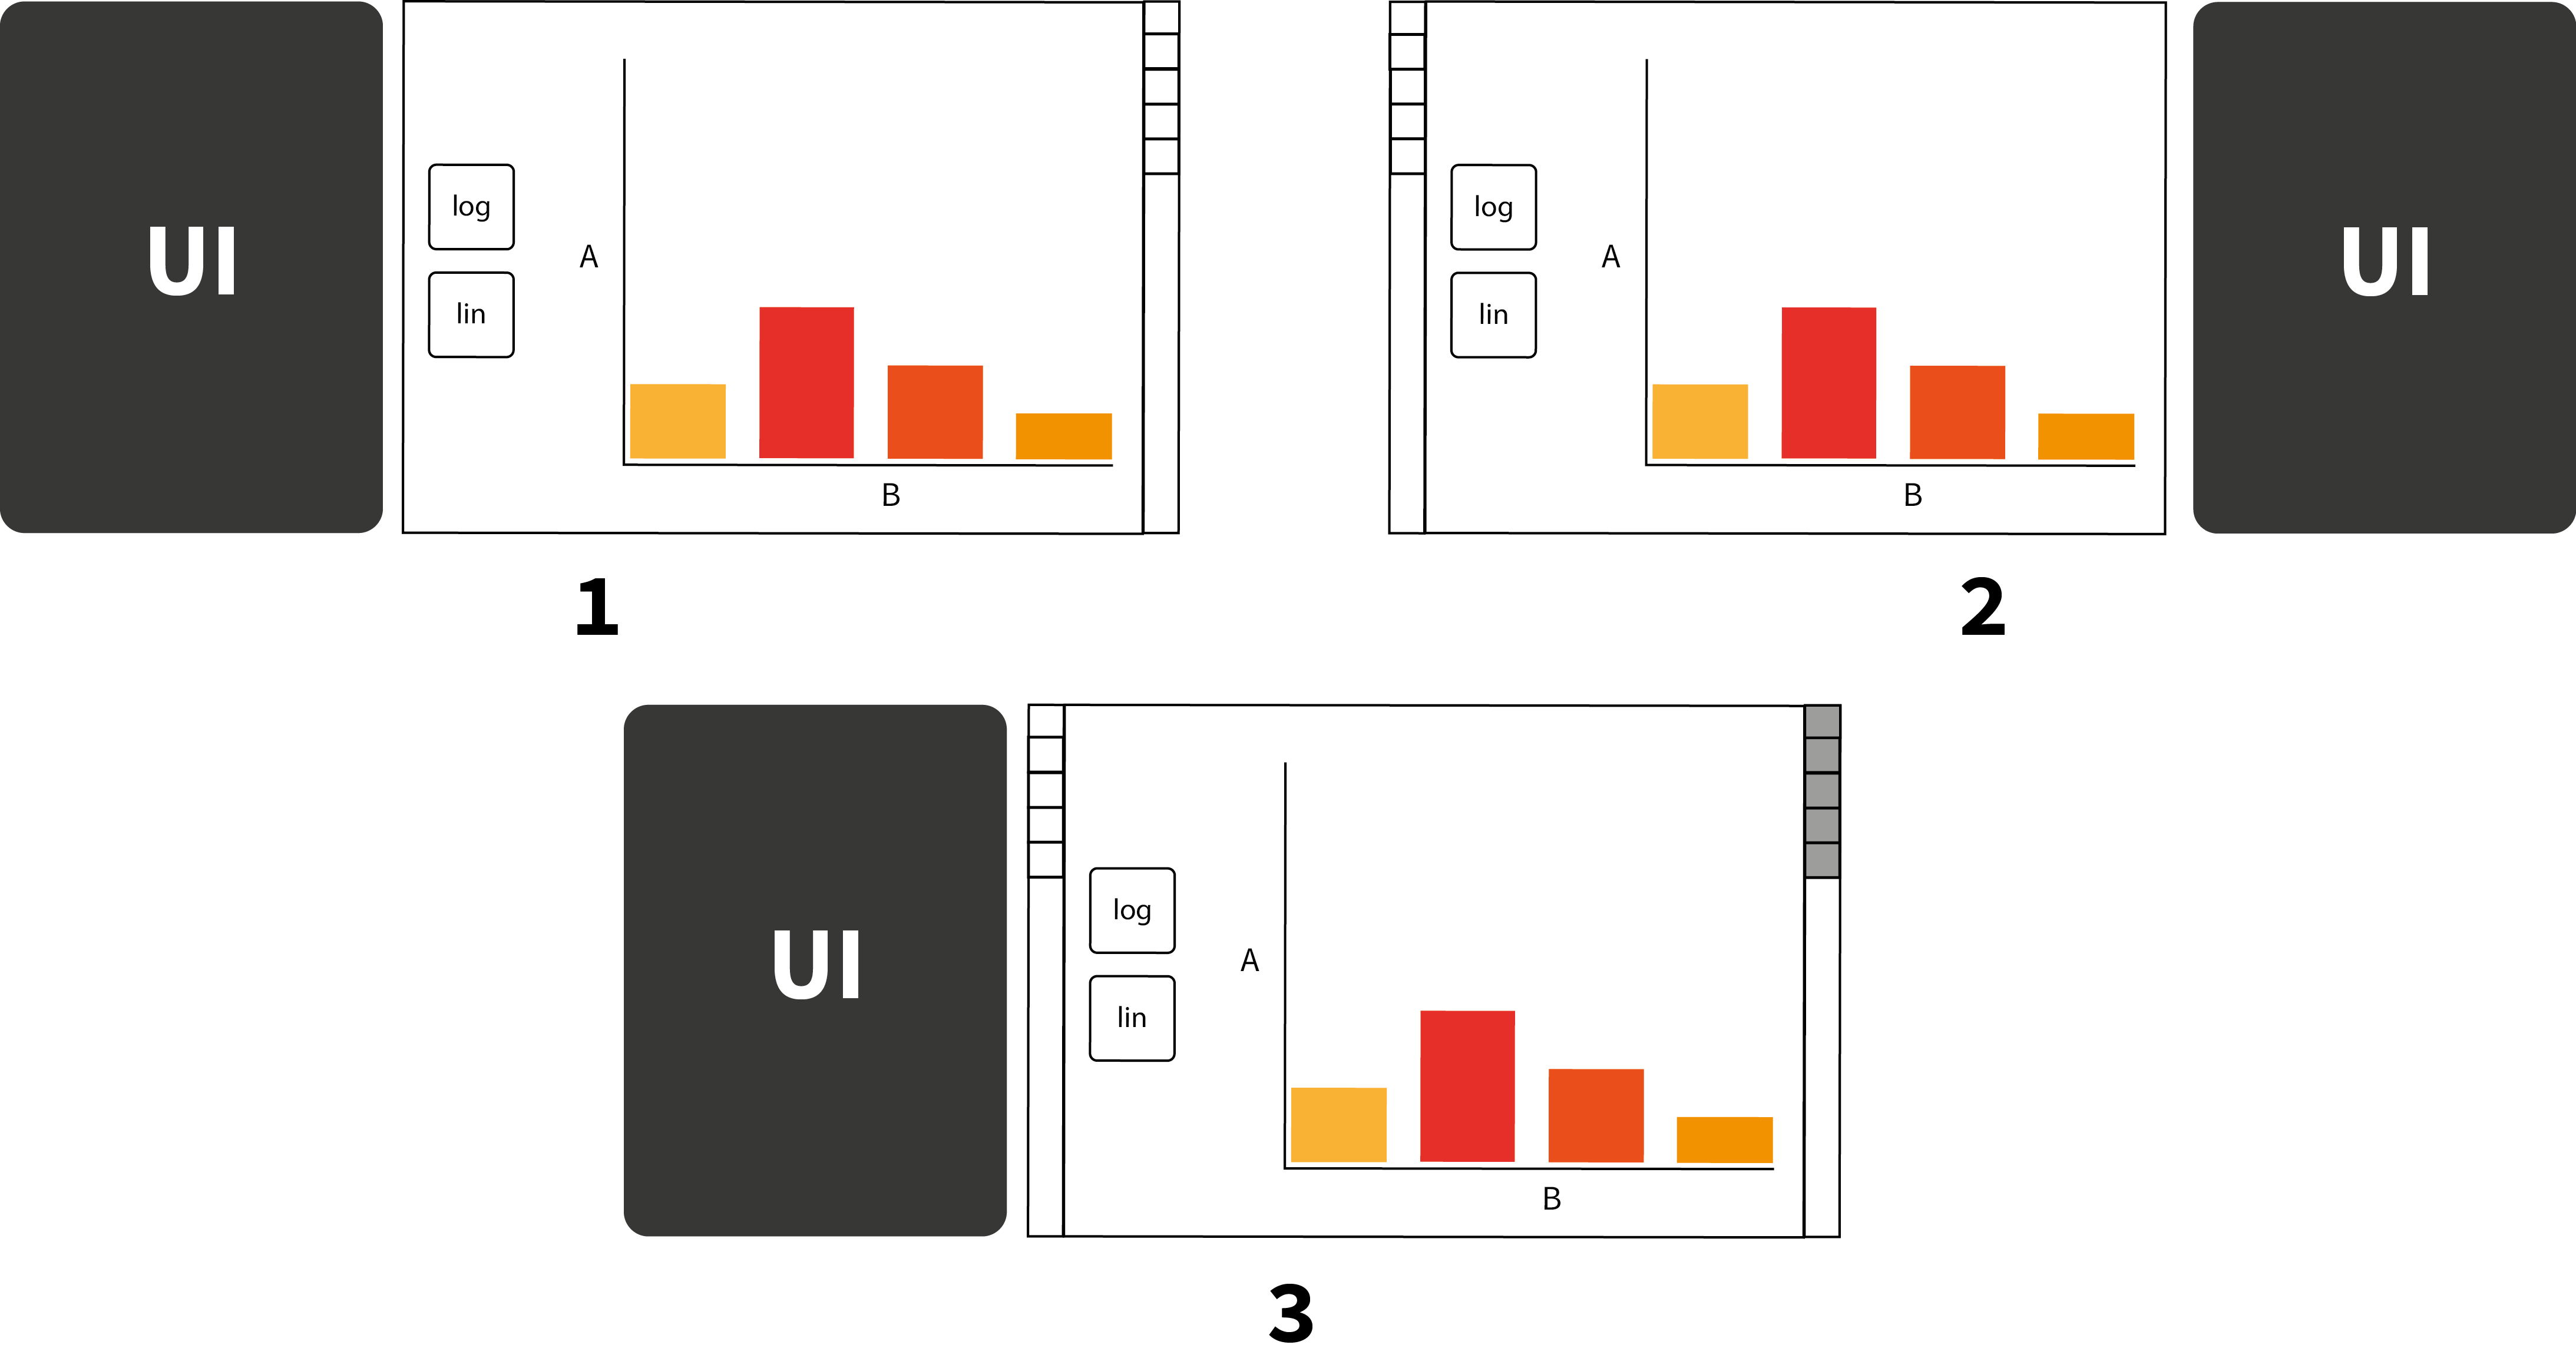
\includegraphics[width=0.5\textwidth]{images/konzeption-ui-buttonleiste.png}
   \caption{Alternative zu Buttons in der Titelleiste}
   \label{figure:ui-buttonleiste}
\end{figure}

\subsubsection{Optik}

Visuelle Konsistenz ist wichtig, damit der Benutzer Elemente gleichen Typs erkennen kann (Abschnitt~\ref{section:standderforschung:verwandte_arbeiten}). Deswegen hat der Bereich, in der Hilfefunktionen angezeigt werden, abgerundete Ecken. So hebt sich die UI für Hilfe von der normalen UI der Komponente, welche spitze Ecken aufweist, ab. Aus demselben Grund wird für die Hilfe UI ein dunkler Hintergrund gewählt, da der Hintergrund von VizBoard weiß ist. Um etwas hervorzuheben, wird prinzipiell die Farbe Orange benutzt, da dies im bestehenden VizBoard Farbschema so festgelegt wurde. Eine Überlagerung der Komponente mit einem leichten Grau dient der Blickführung zu einem nicht überlagerten Element. Ist die Komponente hingegen mit einem tiefen Grau überlagert, signalisiert die dunkle Fläche eine \enquote{No Click Area}, wo keine Interaktionen ausgeführt werden können. 

Offensichtlich sind die gewählten visuellen Effekte nicht mehr so nützlich, wenn eine Komponente einen dunklen Hintergrund aufweist. Schwarz mit Dunkelgrau zu überlagern macht für das menschliche Auge nur wenig Unterschied. Deswegen werden in diesem Fall dieselben Effekte mit Weiß und Hellgrau verwendet.

\subsection{Nutzerstudie}
\label{section:konzeption:einleitung:nutzerstudie}

Das entworfene Konzept wurde mit einer formativen Nutzerstudie evaluiert und danach entsprechend überarbeitet. Die wichtigste zu beantwortende Frage war dabei, ob die Kommunikationshilfe statisch (d.\,h. nach Klick auf einen Button) oder dynamisch (d.\,h. sobald eine Nachricht zwischen Komponenten ausgetauscht wurde) aufgerufen werden soll. Dazu wurde ein Paper Mockup \cite{Virzi1996} erstellt (Abbildung~\ref{figure:paper-mockup}). Er besteht aus einem Balkendiagramm, einer Karte und einer Tabelle. Als Datengrundlage wurden NBA Spieler gewählt. Die Balken des Balkendiagramms konnten ausgewählt werden, woraufhin sich die Tabelle und die Karte anpassten.

\begin{figure}[htbp]
   \centering
   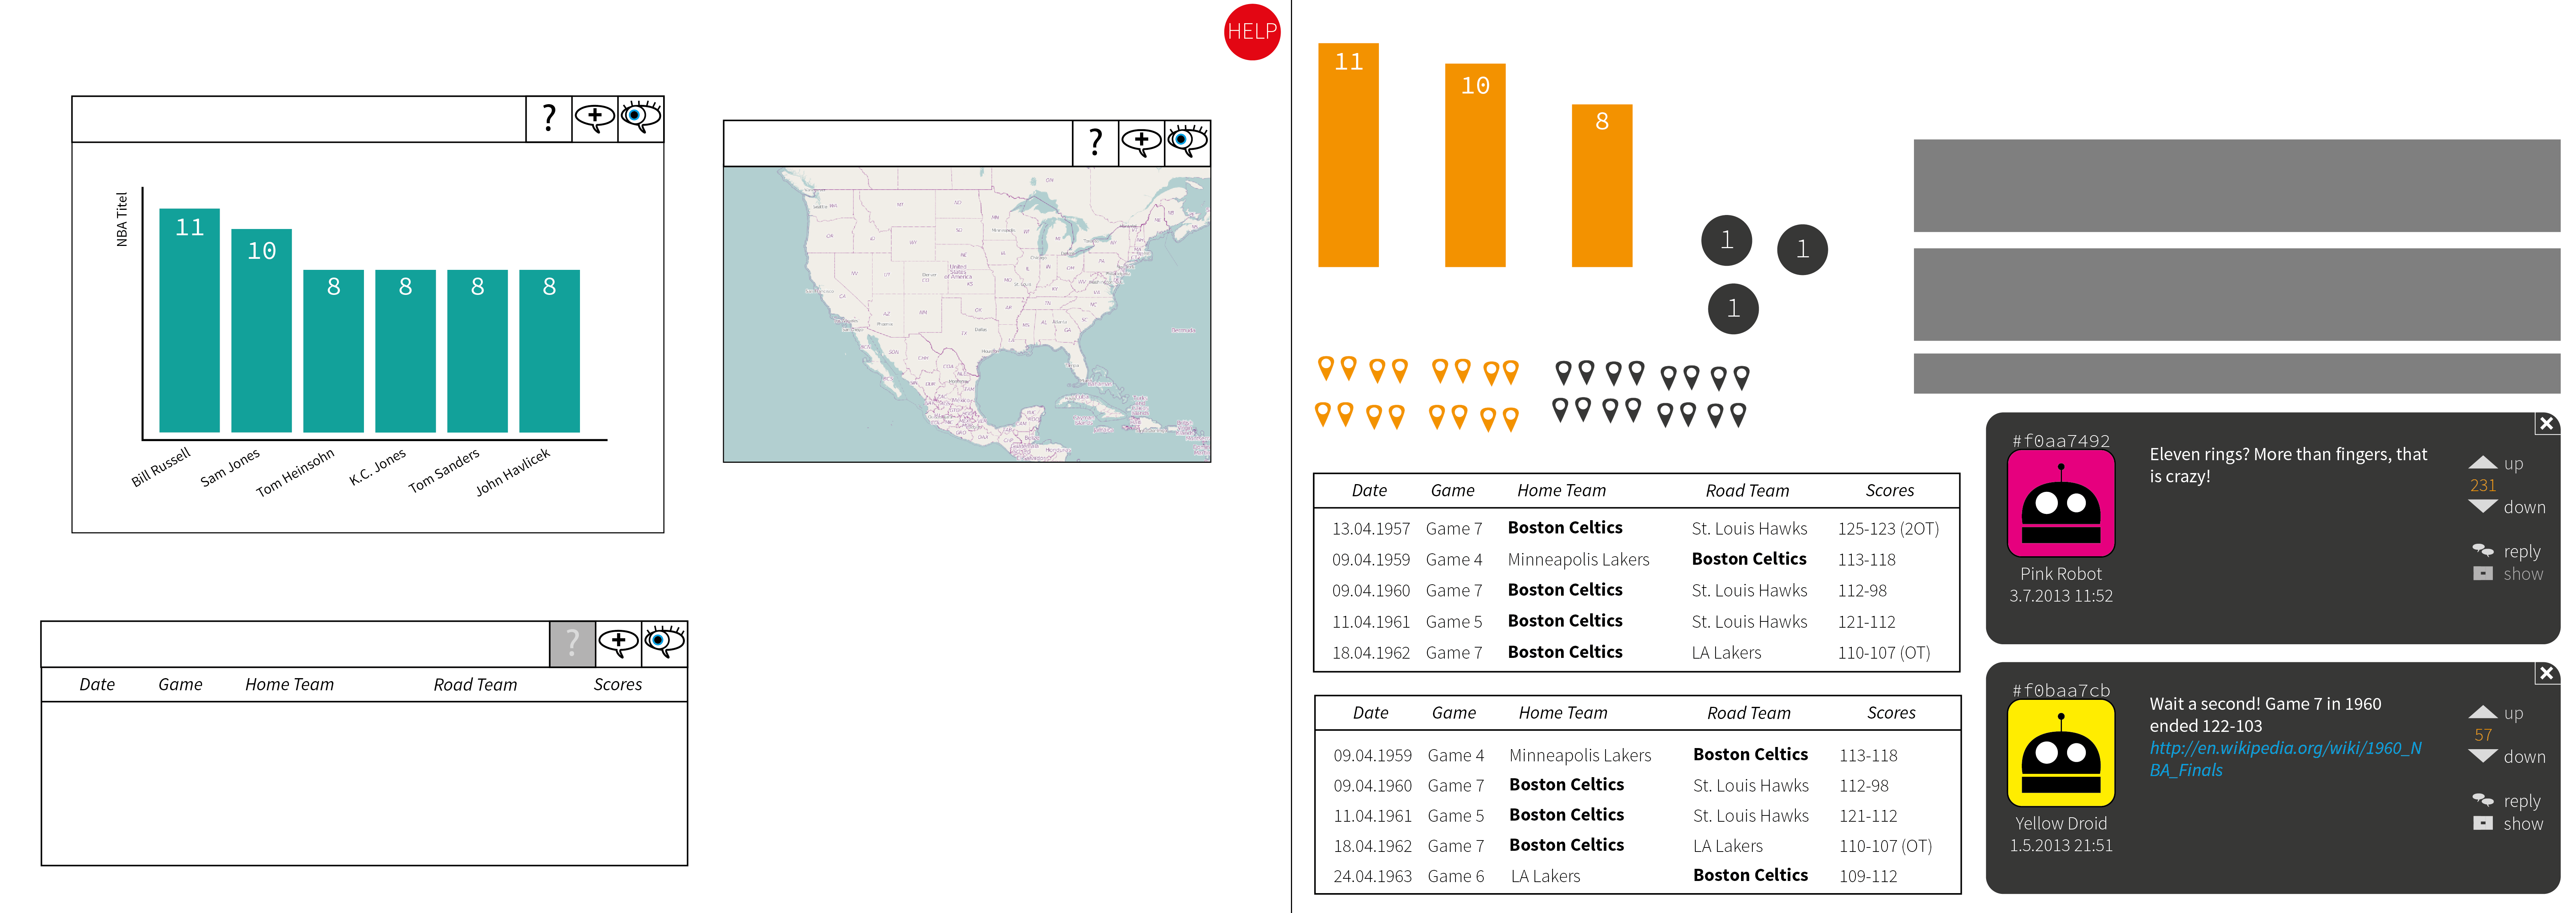
\includegraphics[width=\textwidth]{images/konzeption-paper-mockup.png}
   \caption{Die ersten zwei Seiten des Paper Mockups}
   \label{figure:paper-mockup}
\end{figure}

\subsubsection{Teilnehmer}

Die Nutzerstudie wurde mit fünf Teilnehmern zwischen 23 und 25~Jahren durchgeführt (Tabelle~\ref{table:mockup:teilnehmer}). Dabei waren 60~\% der Personen männlich. Bei der Auswahl der Probanden wurde darauf geachtet, dass beide Geschlechter und auch andere Domänen außer Informatik vertreten sind.

\begin{table}[htbp]
	\centering
    \begin{tabular}{c|c|c|c}
    Teilnehmer   & Geschlecht & Alter & Domäne      \\
    \hline
    Teilnehmer 1 & M          & 25    & Informatik  \\ %fabi
    Teilnehmer 2 & W          & 23    & Zahnmedizin \\ %anna
    Teilnehmer 3 & M          & 23    & Informatik  \\ %kirsche
    Teilnehmer 4 & M          & 25    & Informatik  \\ %sebastian
    Teilnehmer 5 & W          & 25    & Zahnmedizin \\ %karo
    \end{tabular}
    \caption{Teilnehmer der Nutzerstudie}
    \label{table:mockup:teilnehmer}
\end{table}

\subsubsection{Methode}

% einführung

Zuerst wurde den Teilnehmern eine einführende Erklärung gegeben, wie sie später die Einführung in eine Komponente (Abschnitt~\ref{section:konzeption:intro}) übernehmen soll. Dabei wurde der Typ des Diagramms erklärt (wenn notwendig) und die enthaltenen Daten erwähnt. Über die Kommunikation zwischen Komponenten wurde keine Aussage gemacht, einige Teilnehmer konnten allerdings einfach schließen, dass diese in irgendeiner Form stattfinden musste. 

% ablauf

Nach der Einführung sollten die Testpersonen die Anwendung benutzen, wobei zwei mögliche Fragestellungen erwähnt wurden, denen sie nachgehen konnten. MouseOver-Interaktionen wurden explizit beschrieben, da sie im Paper Mockup nicht sichtbar sind. Die Probanden wurden gebeten, während der Nutzung ihre Gedanken laut mitzuteilen (\enquote{Thinking Aloud} Methode \cite{vanSomeren1994}). Im Laufe des Tests wurden die Teilnehmer beispielsweise gefragt, warum sie bestimmte Dinge annahmen, ob die gezeigten Informationen ausreichen, welche Interaktionsmöglichkeiten sie in einer Situation sahen, welche Veränderungen sie erwarteten oder ob eine alternative Interaktion beziehungsweise ein verändertes User Interface besser geeignet wäre. Wenn sie eine Funktion nicht von selbst wählten (etwa einen Kommentar zu verfassen), wurden sie darauf hingewiesen, sodass jeder Teilnehmer alle Funktionen benutzte.

\begin{figure}[htbp]
   \centering
   \includegraphics[width=0.5\textwidth]{images/konzeption-paper-mockup-anna.jpg}
   \caption{Eine Teilnehmerin der Nutzerstudie}
   \label{figure:paper-mockup-anna}
\end{figure}

Um die Hauptfrage, ob Kommunikationshilfe (Abschnitt~\ref{section:konzeption:kommunikation}) statisch oder dynamisch präsentiert werden soll, zu klären, wurde die dynamische Variante drei der fünf Teilnehmer gezeigt. Die anderen zwei testeten die statische Kommunikationshilfe. Alle Teilnehmer wurden am Ende gefragt, ob ihnen die Alternative mehr geholfen hätte.

\subsubsection{Einschränkungen}

% generelle nachteile von thinking aloud
% sehr kleiner mockup
% kein hover, kein scrollen, kein zoomen, keine transparenz...

Die gewählte Methode weist gewisse Einschränkungen auf, denen man sich bei der Auswertung bewusst sein sollte. Einerseits werden Teilnehmer bei \enquote{Thinking Aloud} doppelt belastet. Sie müssen sowohl ein unbekanntes User Interface benutzen, was mentalen Aufwand darstellt, als auch gleichzeitig ihre Gedanken formulieren. Das kann zu Inkonsistenzen in ihren Äußerungen führen.

Andererseits war der Mockup sehr klein, er beinhaltete nur drei Komponenten und zwei Kommunikationskanäle. Gerade letztere konnten die Teilnehmer auch ohne Hilfe verstehen, da sich der \enquote{Bildschirm} nur langsam und schrittweise änderte. Außerdem bezogen sich die Äußerungen und Vorschläge nur auf die vorgestellten Komponenten, ohne Alternativen zu berücksichtigen (beispielsweise Scatterplots, Parallel Coordinates etc.).

Zuletzt liegt es in der Natur des Paper Mockups, dass Interaktionen wie MouseOver, scrollen, zoomen oder draggen nur mit viel Aufwand umgesetzt werden können. Da dies im beschriebenen Mockup nicht der Fall war, konnte die Wirksamkeit dieser Interaktionen nicht überprüft werden.

\subsubsection{Ergebnisse}


% Dass Comic = Beschreibung nicht offensichtlich. Mehr beschreiben, in Zukunft vielleicht auch schickeret Panel-Layout, sodass er als Comic und nicht als Reihe von Bildern identifiziert wird. Basti meinte auch, dass Pfeile als letzter Schritt markiert werden sollten, weil er das so als entweder/oder sah. Weiters meinen einige, dass Panels 3-5 ausreichen. Basti sagt, dass zeitlicher Abstand, also quasi Reihenfolge besser deutlich gemacht werden sollte.
% Statische Hilfe hat gewonnen, aber siehe Einschränkungen. Vielleicht macht man in Zukunft einen Threshold, ab dem dynamische Komm.hilfe verwendet wird? Kann man ja in einer weiteren Nutzerstudie austesten, wo die Grenze liegt.
% Dass Kommentare Annotationen enthalten können, war nicht ohne Erklärung klar. Auch nicht, wie man sie hinzufügt --> Ins Intro.
% Auge-Icon versteht irgendwie keiner.
% Voting war nicht klar, Assoziationen mit scrollen. Was mich vor allem bei Typen wundert, die vermutlich täglich bei StackOverflow reinschauen (müssen).
% Wie mit Kommentaren umgehen, die keine Annotationen enthalten? Basti: Badge an Visualisierung.
% Kommentar-Badges ohne Toggle Button? Ich find ja nicht, weil die übelst ablenken können (Scatterplot)
% Brief-Icon war nicht klar, Assoziationen mit Email und Facebook
% Animation von Mauszeiger in Comics: Ausblick.
% Auswahlhilfe für Annotationen: Ausblick.

Zwei der Teilnehmer konnten sofort erkennen, dass die vier Panels der Bedienungshilfe (Abschnitt~\ref{section:konzeption:bedienung}) einen Comic und dieser wiederum eine Anleitung darstellte. Das sollte zusätzlich mit Text beschrieben werden. Außerdem könnte ein ansprechenderes Layout der Panels dazu führen, dass sie mehr als Comic und weniger als vier unabhängige Bilder wahrgenommen werden. Einer der Teilnehmer merkte zusätzlich an, dass nicht ganz klar ist, ob der durch die Pfeile der statischen Kommunikationshilfe (Abschnitt~\ref{section:konzeption:kommunikation}) angedeutete Nachrichtenaustausch immer, nacheinander oder gleichzeitig stattfindet. Nachdem das für das Hilfesystem auch nicht eindeutig ist, kann in dieser Hinsicht leider nicht viel getan werden. Vier der fünf Teilnehmer waren sich einig, dass die letzten drei Panels des Comics auch ausreichen würden, da die Information in den ersten beiden redundant ist: Durch die Auswahl des Pfeils ist klar, um welche Komponenten es geht.

Es gab keinen eindeutigen Sieger bezüglich der Frage, ob die Kommunikationshilfe (Abschnitt~\ref{section:konzeption:kommunikation}) statisch oder dynamisch angeboten werden soll (Tabelle~\ref{table:paper-mockup-kommunikationshilfe}). Jeder Teilnehmer schätzte die jeweilige Variante der Hilfestellung als notwendig ein ($+$) oder nicht ($-$), wobei ein Teilnehmer sich nicht festlegen wollte (0). Insgesamt kann festgestellt werden, dass Kommunikationshilfe notwendig ist. Allerdings waren sich die Teilnehmer uneins, welche Form die Hilfestellung haben sollte: Je ein Teilnehmer fand beide gut oder beide schlecht, zwei bevorzugten die statische Variante und einer die dynamische. Es ist zu beachten, dass diese Anmerkungen nach einer sehr übersichtlichen Situation im Mashup gemacht wurden. Wäre die Nutzerstudie mit mehr Komponenten durchgeführt worden, böte sich wahrscheinlich ein anderes Bild. Deswegen sollten in einer weiteren Nutzerstudie Grenzwerte für die Anzahl an Komponenten und Kommunikationskanälen bestimmt werden, bei denen Benutzer die Kommunikation nicht mehr ohne weiteres nachvollziehen können. Das Hilfesystem kann dann beim Start der kompositen Anwendung entscheiden, ob zusätzlich die dynamische Kommunikationshilfe eingesetzt werden muss.

\begin{table}[htbp]
	\centering
    \begin{tabular}{c|c|c}
    Teilnehmer   & Dynamisch	& Statisch      \\
    \hline
    Teilnehmer 1 & +			& +  \\ %fabi
    Teilnehmer 2 & -         	& +   \\ %anna
    Teilnehmer 3 & -         	& +    \\ %kirsche
    Teilnehmer 4 & +        	& 0  \\ %sebastian
    Teilnehmer 5 & -         	& -      \\ %karo
    \hline
    Gesamt		& -1			& +2 
    \end{tabular}
    \caption{Wertung der Kommunikationshilfe}
    \label{table:paper-mockup-kommunikationshilfe}
\end{table}

Auffallend war außerdem, dass Teilnehmer, wenn sie über notwendige Ausführungsschritte sprachen, ein anderes Vokabular als die Kommunikationshilfe (Abschnitt~\ref{section:konzeption:kommunikation}) benutzten. Anstatt in Operationen (\enquote{hier auf einen Balken klicken}) sprachen sie in Aktionen (\enquote{hier einen Spieler auswählen}). Das lässt darauf schließen, dass das Hilfesystem ebenfalls in Aktionen sprechen sollte, wenn es die Zusammenhänge zwischen Komponenten erklärt, da es eher dem mentalen Modell der Benutzer entspricht (Abschnitt~\ref{section:standderforschung:grundlagen}).

Ein Teilnehmer schlug vor, die verschiedenen Hilfestellungen zur Kommunikation zusätzlich in der ursprünglich für die Bedienung vorgesehenen Sidebar aufzulisten. Dieser Ansatz ist sowohl einfach als auch für Benutzer offensichtlich. Vermutlich könnte diese Liste, welche dann alle Anleitungen zu Aktionen in der Komponente, alle Effekte von ausgehenden Nachrichten und alle Reaktionen auf eingehende Nachrichten enthielte, schnell sehr lang werden. Es ist zu befürchten, dass Benutzer in diesem Fall die Liste wegen zu viel dargestellter Information gar nicht mehr beachten. Deshalb wird dieser Vorschlag vorerst nicht umgesetzt.

Den Teilnehmern war nicht allein aufgrund der UI klar, dass Kommentare (Abschnitt~\ref{section:konzeption:kommentare}) Annotationen enthalten können und wie diese hinzugefügt oder angezeigt werden. Die Kommentare sollten deswegen am Ende des Intros (Abschnitt~\ref{section:konzeption:intro) zusätzlich erklärt werden. Dasselbe Problem war bei der Bewertungsfunktion von Kommentaren zu beobachten. Die abstrakten, von StackOverflow\footnote{\url{http://stackoverflow.com}} inspirierten Icons wurden auch von Informatikern teilweise mit \enquote{scrollen} anstatt \enquote{bewerten} assoziiert. Deswegen sollte noch einmal explizit mit Text beschrieben werden, dass sie eine Bewertungsfunktion darstellen und welche Semantik sich hinter ihnen verbirgt (\enquote{agree/disagree}). Falls die Funktionalität dann immer noch nicht verständlich ist, können die abstrakten Icons durch Daumen hoch/runter ersetzt werden. Eine weitere Erkenntnis diesem Sachverhalt ist, dass Scrollmöglichkeiten immer explizit dargestellt werden sollten. Das kann entweder in Form einer Scrollbar oder wie im Metro User Interface von Windows Phone~7 mit angeschnittenen Interaktionselementen passieren.

Von zwei Teilnehmern kam der Vorschlag, die Anzahl der Kommentare (Abschnitt~\ref{section:konzeption:kommentare}) in einer Visualisierung ständig darzustellen und nicht über einen Button in der Titelleiste zu toggeln. Hier ist aber zu beachten, dass die Komponenten im Paper Mockup sehr einfach gehalten waren und sehr eingeschränktes Interaktionspotential boten. Bei einem großen Scatterplot oder Parallel Coordinates ist diese Variante nicht mehr praktikabel. Aufgrund des Ziels der \emph{Einheitlichkeit} sollten auch keine Ausnahmen gemacht werden.

Weitere Vorschläge, die hier den Rahmen sprengen würden und in weiteren Arbeiten behandelt werden können, beinhalten zusätzlich einen Mauszeiger im Comic zu animieren oder Vorschläge für mögliche Auswahlrechtecke bei den Annotationen anzubieten.

\section{Intro in die Funktionalität einer Komponente}
\label{section:konzeption:intro}

Aus dem Szenario (Abschnitt~\ref{section:standderforschung:szenario}) und den verwandten Arbeiten (Abschnitt~\ref{section:standderforschung:verwandte_arbeiten}) wurde deutlich, dass dem Endnutzer zuerst ein Überblick über die verschiedenen ausgewählten Komponenten gegeben werden muss, sodass ihm die Struktur der kompositen InfoVis klar wird. Diese beinhaltet folgende Punkte.

% was kommt rein?

\begin{enumerate}
	\item Art der Visualisierung, z.\,B. \enquote{Balkendiagramm}
	\item Beschreibung der Visualisierung, z.\,B. \enquote{Ein Diagramm, das durch auf der x-Achse senkrecht stehende, nicht aneinander grenzende Rechtecke die Häufigkeitsverteilung einer diskreten Variable veranschaulicht.}
	\item Informationen über enthaltene Daten, z.\,B. BIP auf der y-Achse und Länder auf der x-Achse.
	\item Links zu Tutorials, Videos und Erklärungen
	\item Vor- und Nachteile der ausgewählten Visualisierung, z.\,B. \enquote{übersichtlich, wenn wenige Farben vorhanden sind}
\end{enumerate}

% abgrenzung zu "der dev macht das"
Eine Möglichkeit -- so ist die Beschreibung einer Komponente bereits umgesetzt -- ist den Komponentenentwickler selbst einen Text dazu schreiben zu lassen. Er fügt diesen in die Komponentenbeschreibung ein, von wo das Hilfesystem ihn dann auslesen kann. Allerdings kann auf diese Weise kein \emph{einheitliches} Vokabular bezüglich Informationsvisualisierungen sichergestellt werden. Ein einheitliches Vokabular ist aber wichtig, da unterschiedliche Bezeichnungen derselben Konzepte kontraproduktiv für das Verständnis sind. Deswegen werden die Informationen direkt zu den entsprechenden Konzepten in der VISO hinzugefügt. Von dieser zentralen Stelle kann das Hilfesystem sie dann auslesen und anzeigen, sodass die verwendeten Vokabeln konsistent bleiben. Außerdem kann eine einheitliche Beschreibung die Forderungen nach \emph{Vollständigkeit} und \emph{Korrektheit} erfüllen.

% was bleibt draußen?

% links zu externen quellen
Nach Grammel \cite{Grammel2012} können Links zu Tutorials und Erklärungen hilfreich sein, Endnutzern Visualisierungen zu erklären. Da externe Quellen aber nicht durch das Hilfesystem kontrolliert werden, kann es nicht sicherstellen, dass überall ein einheitliches Vokabular benutzt wird. Wie bereits erwähnt ist ein konsistentes Vokabular wichtig für effektive Hilfestellungen, weswegen dieser Punkt in dieser Form nicht umgesetzt werden kann. Was allerdings möglich ist, sind vom VizBoard-Betreiber erstellte Tutorialvideos in Form von vertonten Animationen, die Aufbau und Vor- bzw. Nachteile grafischer Repräsentationen erklären. Das sind zwar viele Videos, aber die Anzahl der Repräsentationen ist endlich und nicht alle sind gleich wichtig\footnote{Ein Balkendiagramm ist gängiger und deswegen leichter verständlich als eine Scatterplot Matrix.}, weswegen der nötige Aufwand gerechtfertigt scheint.

% vor- und nachteile
Grammel schreibt ebenfalls, dass InfoVis-Novizen die Vor- und Nachteile von verschiedenen Visualisierungstypen und visuellen Mappings lernen sollten \cite[S. 125]{Grammel2012}. Es wäre möglich, allgemeine Eigenschaften von grafischen Repräsentationen in der VISO zu beschreiben. Diese sind abhängig von den dargestellten Daten und den visuellen Mappings. Die Eigenschaft \enquote{Übersichtlichkeit} ist bei einem Balkendiagramm mit drei Balken gegeben (Vorteil), bei 15 Balken nicht (Nachteil). Ähnlich verhält es sich mit der Farbkodierung: Ein Mensch kann bis zu acht Farben in einer Visualisierung gut unterscheiden (Vorteil) \cite{Mazza2009}, aber mehr nicht (Nachteil). Das Hilfesystem müsste dem Benutzer demnach sowohl die unterschiedlichen Vor- und Nachteile als auch deren Bedingungen präsentieren, was sehr viel Information für eine Einführung darstellt. Im schlechtesten Fall kann der Benutzer auch keinen Bezug zur konkreten Visualisierung herstellen, weil keine der aufgeführten Bedingungen erfüllt ist. Er kann die aufgestellte Hypothese nicht am Beispiel überprüfen, was laut Grundlagen schlecht für seinen Verständnisprozess ist (Abschnitt~\ref{section:standderforschung:grundlagen:user_assistance:sensemaking}). Hinzu kommt, dass diese Erklärung einen Schritt früher im VizBoard Workflow konzeptionell mehr Sinn macht. Dort wählt der Benutzer -- von VizBoard unterstützt -- die visuellen Mappings aus.

Aus den eben aufgeführten Gründen zeigt das Intro für eine Komponente folgende Informationen:

\begin{enumerate}
	\item Art der Visualisierung
	\item Beschreibung
	\item Enthaltene Daten
	\item Tutorialvideo, wenn vorhanden
\end{enumerate}

Davon ist Punkt~3 spezifisch für die Domäne der Informationsvisualisierung, da CRUISe Komponenten keine Daten visualisieren müssen. Die anderen Punkte sind für alle auf CRUISe basierenden Mashups hilfreich.

% interaktionshilfen - kommen später

Über die Interaktion mit der Visualisierung wird hier noch keine Aussage gemacht, da sie sehr umfangreich sein kann und den Rahmen des Intros sprengen würde. In Abschnitt~\ref{section:konzeption:bedienung} wird eine Hilfestellung zur Bedienung einer Komponente erarbeitet.

\subsection{User Interface und Interaktion}
\label{section:konzeption:intro:ui}

Nachdem der Benutzer bei der Visualisierung angekommen ist und die Komponenten sieht, wird der gesamte Viewport abgedunkelt und eine Sidebar neben der ersten Komponente (von links oben nach rechts unten) eingeblendet (Abbildung~\ref{figure:ueberblick}). Dort sind die im vorigen Abschnitt erläuterten Informationen zu finden: Die Art der Visualisierung (\enquote{Karte}), darunter eine Beschreibung einer Karte, Informationen zu den dargestellten Daten und zuletzt ein Tutorialvideo, wenn vorhanden. So werden die Fragen \enquote{Was ist das für eine Visualisierung?}, \enquote{Wie soll ich sie interpretieren?} und \enquote{Was zeigt sie für Daten?} beantwortet. Mit den Pfeilen links und rechts kann zwischen den Beschreibungen für verschiedene Komponenten gewechselt werden. Über die Meta-Hilfe (Abschnitt~\ref{section:konzeption:meta-hilfe}) kann das Intro wieder aufgerufen werden, wenn es geschlossen wurde.

\begin{figure}[htbp]
   \centering
   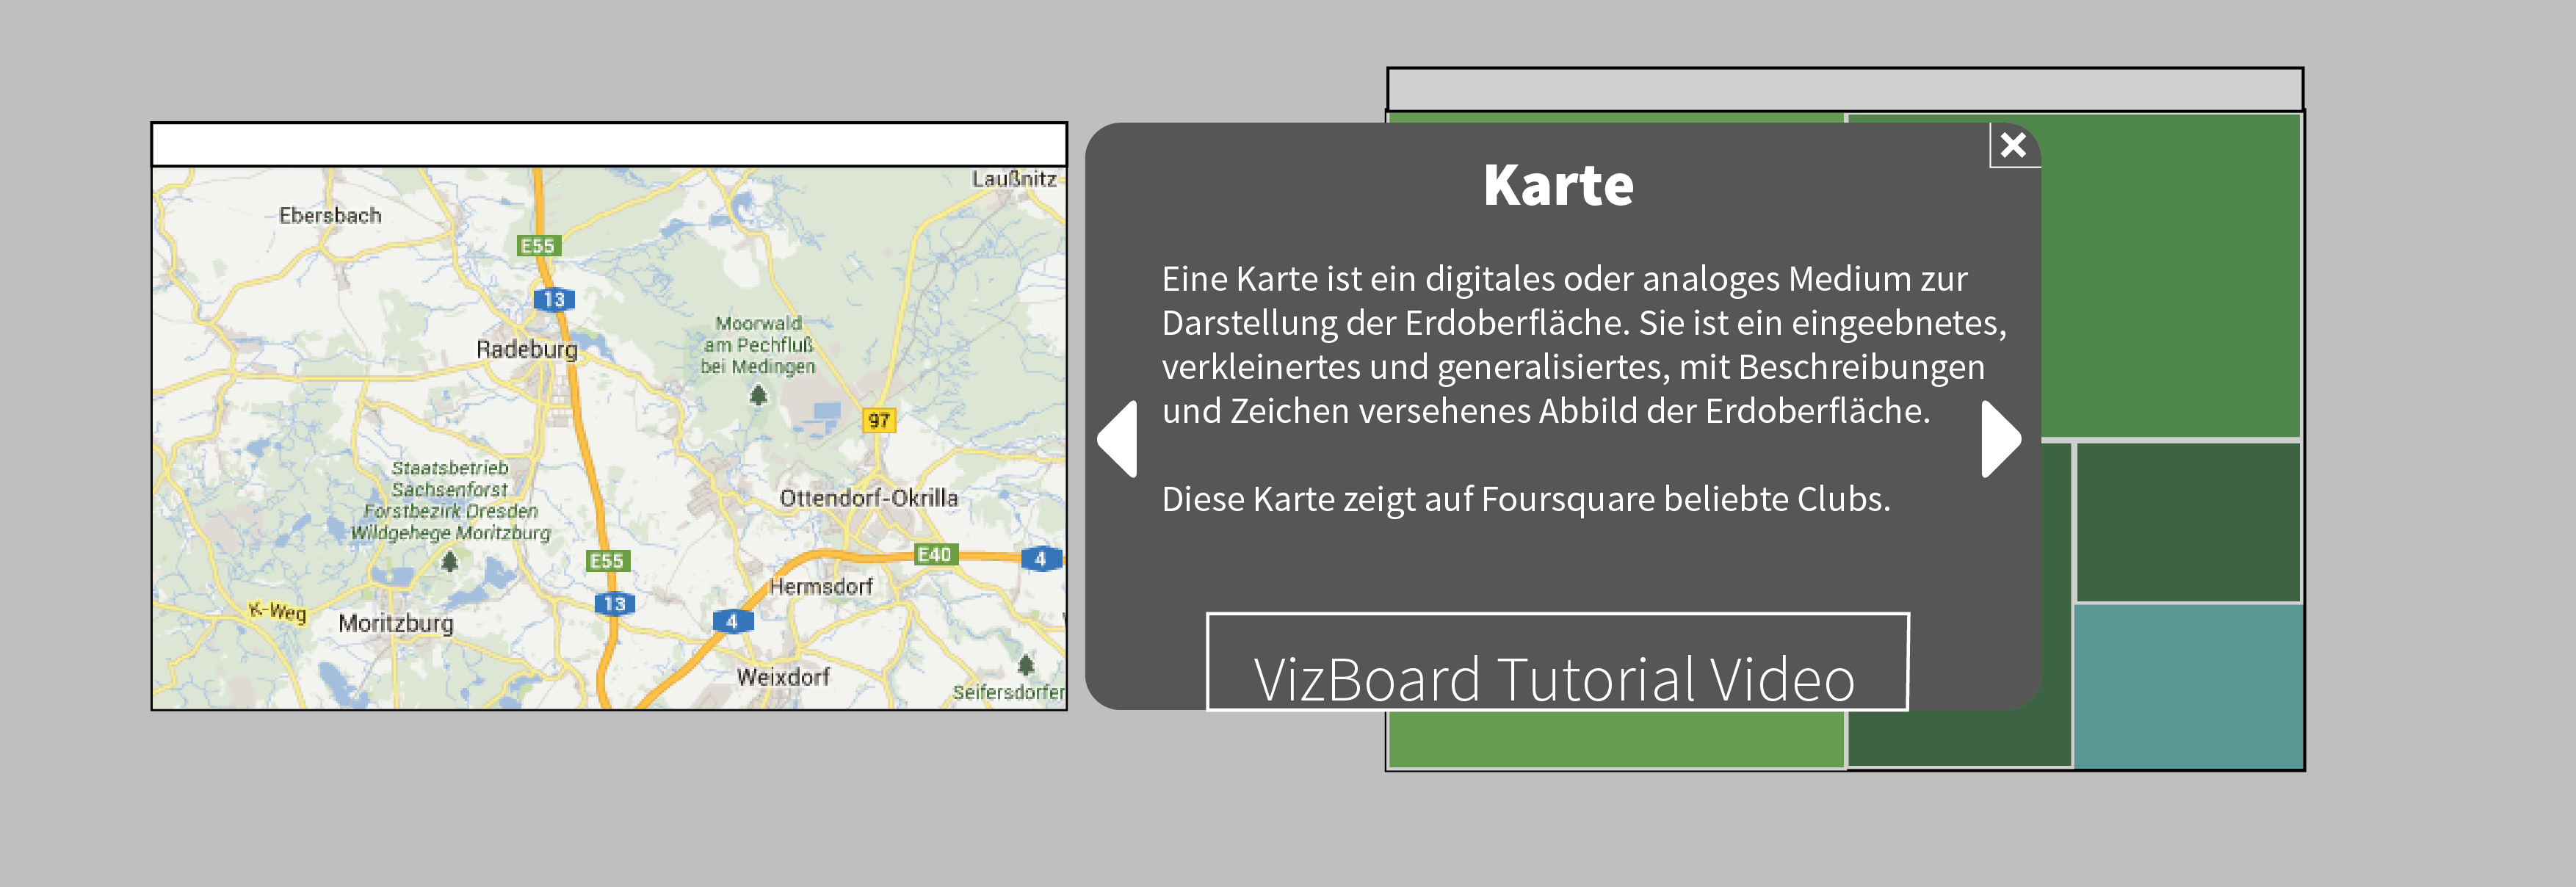
\includegraphics[width=0.75\textwidth]{images/konzeption-ueberblick.png}
   \caption{UI Mockup: Intro}
   \label{figure:ueberblick}
\end{figure}

\subsection{Backend}
\label{section:konzeption:intro:backend}

Die VISO (Abschnitt~\ref{section:standderforschung:grundlagen:cruise_vizboard:viso}) enthält bereits ein Vokabular für Informationsvisualisierungen. Deswegen ist es naheliegend, die Beschreibung der Visualisierung in die VISO hinzuzufügen. Die Art der grafischen Repräsentation muss der Komponentenentwickler bereits jetzt in der Komponentenbeschreibung hinzufügen. Das bedeutet das Hilfesystem kann die entsprechenden Daten auslesen. Die in der Visualisierung verwendeten Daten entsprechen dem Domain Assignment, welches der Komponente von der Laufzeitumgebung mitgeschickt wird. Das Domain Assignment ist das Mapping vom während der Integration erstellten generischen Datenschema auf Konzepte, die in einer externen Wissensbasis wie der DBpedia beschrieben werden \cite{Voigt2012a}.

% core erweiterung

Damit das Hilfesystem aber die URIs der aktuell visualisierten Datatype Properties bekommt, muss das CoRe erweitert werden. Aktuell gehen die URIs bei der Transformation in das generische Datenschema verloren, weil sie umbenannt werden. Um dem Komponentenentwickler Aufwand zu ersparen sollte deswegen das CoRe dahingehend erweitert werden, dass das ursprüngliche Mapping der MRE mitgeliefert wird.


\section{Bedienung einer Komponente}
\label{section:konzeption:bedienung}

In den verwandten Arbeiten (Abschnitt~\ref{section:standderforschung:verwandte_arbeiten}) wurde festgestellt, dass das Hilfesystem den Benutzer über das Verhalten der InfoVis aufklären muss. Da die Komponenten \enquote{Black Boxes} sind und von verschiedenen Entwicklern stammen, kann der Benutzer weder von verfügbaren möglichen Aktionen wie z.\,B. zoomen noch von einheitlicher Gestaltung der Interaktionen ausgehen. Beispielsweise wann eine Interaktion durch \texttt{MouseOver} anstatt \texttt{Click} ausgeführt wird. Deswegen ist eine Hilfestellung zur Bedienung notwendig.

% wieder erste möglichkeit: dev baut selbst hilfe ein. text+bilder: kein einfluss auf wortwahl, art der bilder, ausführlichkeit etc. Comics: für jede aktion eins, übelster aufwand, kann man nicht verlangen, außerdem 2. wer sagt dass ein prof. sw-entwickler das können soll?

Die einfachste Umsetzung der Hilfe zur Bedienung ist dem Komponentenentwickler eine Möglichkeit zu geben, Text und Bilder zu diesem Thema in die Komponentenbeschreibung einzufügen. Das hat allerdings den Nachteil, dass das Hilfesystem keinen Einfluss auf die Wortwahl, Gestaltung der Bilder oder Ausführlichkeit der Erklärung hat (Ziele der \emph{Einheitlichkeit}, \emph{Vollständigkeit}, \emph{Korrektheit}, \emph{Verständlichkeit}).

Hilfestellungen zur Bedienung würden vom Benutzer wahrscheinlich am besten verstanden, wenn sie tatsächlich vorhandene, konkrete Elemente der Komponente verwendete (\enquote{Semantic Transparency} \cite{Kohlhase2009}). Um zu demonstrieren, dass nach einem Klick die Tabelle sortiert sein wird, könnten die Zeilen derselben beispielhaft ihre Position wechseln. Assistance in dieser Form kann auf zwei Arten umgesetzt werden, die beide ihre Nachteile haben.

Einerseits könnten Aktionen mit Hilfe einer festgelegten Grammatik beschrieben werden. Beispielsweise würde die Aktion \enquote{sortieren} beinhalten, dass Elemente in Abhängigkeit eines Attributwerts ihre Position in der Visualisierung ändern. Dann könnte das Hilfesystem selbst die Tabellenzeilen demonstrativ sortieren, da es nun weiß, was die Aktion \enquote{sortieren} bedeutet. Der große Nachteil daran ist, dass es vermutlich immer einen Komponentenentwickler geben wird, der eine unvorgesehene Aktion in seiner Komponente umsetzen will und sie nicht beschreiben kann. Die zweite Lösung, eine semantisch transparente Assistance umzusetzen, ist den Komponentenentwickler für jede Aktion eine Methode in seiner Komponente hinzufügen zu lassen, die diese demonstriert. Zur Laufzeit würde die Methode einfach vom Hilfesystem aufgerufen. Das hat allerdings den Nachteil, dass dem Komponentenentwickler erheblicher Mehraufwand aufgebürdet wird und keine Einheitlichkeit der Assistance garantiert werden kann. Aus diesen Gründen ist eine andere Lösung notwendig.

Wie in den Grundlagen (Abschnitt~\ref{section:standderforschung:grundlagen:user_assistance}) gezeigt, können Comics eine effektive und attraktive Lösung für User Assistance sein. Allerdings stellt es für den Entwickler erheblichen Mehraufwand dar, für jede mögliche Aktion verschiedene Comicpanels zu erstellen. Davon abgesehen können (und sollen) die gestalterischen Fähigkeiten dazu nicht von ihm erwartet werden (\emph{Minimalität}) und das Problem der Kontrolle über den Inhalt ist auch nicht gelöst (\emph{Korrektheit}, \emph{Vollständigkeit}, \emph{Verständlichkeit}).

Aus diesem Grund werden die Comicpanels vom Hilfesystem automatisch erstellt. Es bleibt die Frage der Präsentation: Aus den Grundlagen geht hervor, dass eine multimodale Ausgabe (akustisch-verbal und visuell) zur Lerneffektivität beiträgt. Darauf wird aber aus zwei Gründen verzichtet. Einerseits sollen beide Kanäle gleichzeitig ausgegeben werden. Das ist problematisch, weil vier Panels darzustellen wesentlich schneller möglich ist als eine verbale Erklärung für den Vorgang zu sprechen. Die Darstellung der Panels müsste sich der Audioausgabe anpassen und würde wesentlich langsamer vonstatten gehen. Eine nichtfunktionale Anforderung an die Hilfestellung ist aber, dass der Benutzer die Hilfe schnell aufnehmen und verarbeiten können soll. Zweitens wird automatische Soundausgabe gemeinhin als schlechte Usability angesehen. Hauptsächlich weil der Nutzen von Screenreadern dadurch eingeschränkt wird, aber auch weil der Benutzer automatische Wiedergabe nicht kontrollieren kann und die Audiodaten Bandbreite beanspruchen.

% also bleibt es an uns hängen.

\subsection{API und Komponentenbeschreibung}
\label{section:konzeption:bedienung:api}

% ### daten sammeln

Die VISO enthält im Namensraum \texttt{viso:activity} Konzepte der hierarchischen Aktivitätstheorie nach Kuutti \cite{Kuutti1996}:

\begin{itemize}
	\item \textbf{Aktivitäten} stellen langfristige Ziele des Benutzers dar, die nicht unmittelbar zu Ergebnissen führen (müssen). In Bezug auf das Szenario (Abschnitt~\ref{section:standderforschung:szenario}) wäre die Aktivität von Anna \enquote{mehr über die geografische Verteilung verschiedener Genvariationen lernen}.
	\item \textbf{Aktionen} sind Teilziele der Aktivität. Im Szenario sind das \enquote{VizBoard aufrufen}, \enquote{Komponenten auswählen} etc.
	\item Aktionen bestehen wiederum aus einer Kette von \textbf{Operationen}, also beispielsweise Klicks oder Drags.
\end{itemize}

Für das Hilfesystem sind Operationen und Aktionen relevant, da Aktivitäten nicht beeinflusst werden können. Aktionen einer Komponente sind beispielsweise zoomen, suchen oder filtern; Operationen sind etwa Klicks, Drags oder Multitouch-Gesten.

Die Komponentenbeschreibung gibt bereits Auskunft über die verfügbaren Aktionen in einer Komponente (Capabilities). Es fehlen aber noch Informationen darüber, welche Operationen auf welchen Elementen die Aktion ausführen. Um dem beizukommen, werden Operationen aus der VISO (\enquote{welche Operationen}) zusammen mit CSS Selektoren (\enquote{welche Elemente}) in der Komponentenbeschreibung definiert. Äquivalente Operationen, welche dieselbe Aktion ausführen, werden zusammengefasst. Wenn eine Tabelle sowohl durch einen Klick auf den Spaltenkopf als auch über ein separates Menü sortiert werden kann, werden diese Aktionen als äquivalent zusammengefasst. Sequentielle Operationen werden ebenfalls zusammengefasst, wobei die Reihenfolge im Markup die notwendige Ausführungsreihenfolge darstellt. So können auch zusammengesetzte Operationen, wie beispielsweise für ein HTML \texttt{select} Element nötig, abgebildet werden. Parallele Operationen werden nach demselben Prinzip zusammengefasst, allerdings ist hier die Reihenfolge irrelevant, da sie gleichzeitig ausgeführt werden müssen. Auf diese Weise können zusammengesetzte Operationen der der Art STRG+T abgebildet werden.

Außerdem kann der Komponentenentwickler eine Anzahl von Sekunden definieren, die bei der Generierung der Panels gewartet werden soll. Das ist beispielsweise sinnvoll, wenn längere Animationen zu erwarten sind. Beispielsweise weil der Entwickler UI Elemente innerhalb von fünf Sekunden anstatt 500~Millisekunden einblenden will. Zusätzlich ist es möglich, dass der Entwickler Zusatzinformationen in Stichworten angibt. Zum Beispiel könnte bei einem Balkendiagramm die Skala \enquote{verändert} (Aktion) werden. Dabei ist es wichtig zu wissen, welche Skala verwendet werden wird, z.\,B. linear oder logarithmisch. Der Inhalt dieser Zusatzinformationen kann statischer Freitext oder eine Referenz auf eine Datenvariable im Schema der Komponente sein, deren Label zur Laufzeit angezeigt würde. Nach demselben Prinzip sollten auch Zusatzinformationen über die VISO Operation angegeben werden können. Vor allem bei Tastaturkürzel (z.\,B. j/k für vor/zurück) macht es Sinn, da so nicht für jede Taste eine VISO Operation erstellt werden muss. Die erwähnten Zusätze zur Komponentenbeschreibung sollten allerdings optional sein, falls der Komponentenentwickler keine Hilfe für bestimmte Aktionen anbieten will.

Im folgenden werden die in diesem Abschnitt vorgenommenen Änderungen an der Komponentenbeschreibung noch einmal zusammengefasst:
\begin{itemize}
	\item Zu den Aktionen werden VISO Operationen angegeben, welche diese ausführen. Diese können einfach, sequentiell oder parallel sein.
	\item Zu den VISO Operationen werden CSS Selektoren angegeben, um die relevanten UI Elemente zur Laufzeit finden zu können.
	\item Die VISO Operationen können Zusatzinformationen beinhalten, um sie besser zu definieren. Ein Beispiel ist die Taste zur Operation \enquote{tippen}.
	\item Zu den Aktionen wird eine Anzahl von Sekunden angegeben, welche die Zeit bis zur finalen Änderung des User Interfaces angeben (beispielsweise wenn alle Animationen beendet sind).
	\item Zu den Aktionen können Zusatzinformationen in Form Freitext oder Referenzen auf Datenvariablen angegeben werden, um sie näher zu beschreiben.
\end{itemize}

\subsection{Generierung der Assistance}
\label{section:konzeption:bedienung:generierung}

% ### assistance generieren

% warum müssen wir bilder generieren und wie sehen die aus?

Die User Assistance zur Bedienung soll ein Comic werden, der per Definition wiederum aus mehreren Panels besteht, die Bilder und/oder Text enthalten \cite{McCloud1994}. Die Bilder der Panels können nicht a priori gezeichnet werden, da der Inhalt der Komponenten unbekannt ist (\enquote{Black Box} Prinzip). Aus diesem Grund müssen sie automatisch generiert werden. Die einfachste Möglichkeit dafür sind Screenshots der Komponente.

% wie machen wir das?

Dazu wird ein sogenannter \enquote{Headless Browser} verwendet. Das ist ein programmierbarer Browser ohne grafische Benutzeroberfläche, der z.\,B. Screenshots einer Seite abspeichern oder Testskripte ausführen kann. Beispiele sind unter anderem PhantomJS\footnote{\url{http://phantomjs.org/}}, HTMLUnit\footnote{\url{http://htmlunit.sourceforge.net/}} oder Ghost\footnote{\url{http://jeanphix.me/Ghost.py/}}.

% wie läuft das ab?

Bei der Generierung der Panels ist zuerst das Component Repository beteiligt. Sobald eine Komponente hinzugefügt oder upgedatet wurde, parst das CoRe die entsprechende Komponentenbeschreibung und schickt eine Anfrage an den Hilfeservice. Dieser kann ins CoRe integriert sein, sollte dem \enquote{Separation of Concerns} Designprinzip folgend aber davon getrennt sein, da es schon für Matching, Ranking und Verwaltung der Komponenten zuständig ist. Der Hilfeservice rendert die Komponente mit Hilfe des Headless Browsers in einer CRUISe Testumgebung. Sie besteht aus folgenden Komponenten:

\begin{itemize}
	\item Laufzeitumgebung: Sie ist unter anderem für die Initialisierung und das Layout der Komponenten nötig.
	\item Data Repository: Die Komponente muss Daten darstellen, welche aus dem DaRe kommen können.
	\item Component Repository: Das CoRe enthält alle verfügbaren Komponenten und stellt sie dem Hilfeservice zur Verfügung.
\end{itemize}

Es wurde eben erklärt, dass das DaRe die (Test-)Daten für eine Komponente liefern kann. Der Komponentenentwickler gibt in der Komponentenbeschreibung den gewünschten Datensatz und die zu visualisierenden Daten in Form einer SPARQL Query an, welche die Laufzeitumgebung bei der Generierung der Assistance der Komponente zur Verfügung stellt. Das kann ein \enquote{echter} Datensatz oder ein vom VizBoard-Betreiber zur Verfügung gestellter Testdatensatz sein. Es kann allerdings passieren, dass das DaRe keine passenden Daten enthält, weil die Komponente sehr spezielle Daten visualisiert (z.\,B. 3-Sterne-Hotels in Andorra). Dann sollte der Komponentenentwickler zusammen mit der Komponente Testdaten hochladen können oder eine URL angeben, unter der sie zu finden sind. Das ist zwar etwas Mehraufwand, aber es kann angenommen werden, dass im Laufe der Entwicklung einer Komponente sowieso Testdaten verwendet wurden. Sie müssen in den meisten Fällen also nicht mehr erstellt, sondern nur noch hochgeladen werden. Die Bedienungshilfe kann für alle auf CRUISe basierenden Mashups hilfreich sein. Allerdings kann nicht davon ausgegangen werden, dass diese über ein Data Repository verfügen. Dann muss der Komponentenentwickler in jedem Fall Testdaten zur Generierung der Hilfe zur Verfügung stellen.

Nachdem die Komponente von der Laufzeitumgebung vollständig initialisiert und integriert wurde, führt der Hilfeservice folgende Schritte aus:

\begin{enumerate}
	\item Erstelle einen Screenshot vom Ausgangszustand der Komponente
	\item Für jede verfügbare Aktion:
	\begin{enumerate}
		%\item Finde die Bounding Box der relevanten Elemente
		\item Für alle äquivalenten Operationen:
		\begin{enumerate}
			\item Für jede Operation:
			\begin{itemize}
				\item Finde die Bounding Box der betroffenen Elemente und speichere sie
				\item Hebe betroffene Elemente hervor
				\item Erstelle einen Screenshot der Komponente
				\item Setze Zustand der betroffenen Elemente zurück
			\end{itemize}
		\end{enumerate}
		\item Führe die Aktion aus
		\item Warte die definierte Anzahl an Sekunden
		\item Erstelle einen Screenshot vom Ergebnis der Aktion
	\end{enumerate}
\end{enumerate}

Falls die Operation in Schritt 2.a.i sequentiell sein sollte, muss der beschriebene Algorithmus die Bounding Box der Elemente jeder Teiloperation finden, genauso bei parallelen Operationen.

% hell und dunkel unterscheiden

Nachdem alle nötigen Screenshots der Komponente erstellt wurden, muss das Hilfesystem eine Kategorisierung in \enquote{helle Komponente} und \enquote{dunkle Komponente} vornehmen. Das ist nötig, damit das Hilfesystem zur Laufzeit weiß, ob es dunkle oder helle visuelle Effekte einblenden soll. Eine naive Möglichkeit dazu wäre mit Hilfe einer Bildverarbeitungsbibliothek wie OpenCV\footnote{\url{http://opencv.willowgarage.com/wiki/}} die Screenshots zu binärisieren, also in Bilder aus schwarzen und weißen Pixeln umzuwandeln. Enthält die Mehrzahl der Bilder mehr schwarze als weiße Pixel, wird die Komponente als \enquote{dunkel} eingestuft, ansonsten als \enquote{hell}.

% anbieten der assistance diskutieren: bilder in smcdl einbinden, eigener webservice, core.

Die Bilder der Comics können auf unterschiedliche Weise ans Hilfesystem ausgeliefert werden. Eine Möglichkeit ist die Bilder nach Generierung in der Komponentenbeschreibung zu definieren, so wie es bereits mit einem Screenshot der Komponente gemacht wird. Ebenso könnte ein Webservice die Bilder über eine REST API anbieten, von wo das Hilfesystem sie zur Laufzeit lädt. Dieser Webservice kann eigenständig oder im CoRe integriert sein.

\subsubsection{Einschränkungen}
\label{section:konzeption:bedienung:generierung:einschraenkungen}

% nachteile

Die vorgestellte Lösung hat auch Nachteile. Zunächst ist sie vom Document Object Model (DOM) abhängig, was eine automatische Hilfegenerierung für Komponenten ausschließt, die auf Flash, Silverlight oder ähnlichen Technologien basieren. Der Trend geht aber ohnehin zu HTML/SVG-basierten Visualisierungen (z.\,B. mit D3 \cite{Bostock2011} oder Raphaël\footnote{\url{http://raphaeljs.com/}}): Flash ist laut Adobe hauptsächlich für Videoauslieferung und Spiele gedacht \cite{Adobe2013} und Microsoft zieht HTML5 Silverlight vor \cite{Foley2010}. Deswegen sollte dieser Nachteil nicht ins Gewicht fallen.

Eine weitere Einschränkung ist, dass zeitabhängige Interaktionen wie zum Beispiel \enquote{MouseOver für 3 Sekunden} nicht modelliert werden können. Diese sind im Web aber ohnehin eher unüblich und werden als schlechte Usability betrachtet, weil sie nicht sichtbar und deswegen schwer zu entdecken sind.

\subsection{User Interface und Interaktion}
\label{section:konzeption:bedienung:ui}

% ### assistance anbieten

Die Hilfestellung zur Bedienung kann über einen ?-Button in der Titelleiste aufgerufen werden, den der Benutzer vielleicht von nativen Desktop-Applikationen kennt (Abbildung~\ref{figure:bedienung-step1}). Der Viewport der Komponente wird abgedunkelt und nur die Elemente, für die auch Hilfestellungen existieren, bleiben sichtbar. Neben der Komponente erscheint eine Sidebar, welche die verfügbaren Aktionen noch einmal auflistet. Die Assistance wird entweder nach einem Klick auf ein sichtbares UI Element oder ein Element der Liste aufgerufen. So kann der Benutzer sowohl die Frage \enquote{Was macht dieser Button?} als auch \enquote{Wie kann ich Aktion XY ausführen?} beantworten. Eine zweite Möglichkeit, wie die Assistance aufgerufen werden kann, ist über einen ?-Button am Interaktionselement selbst (Abschnitt~\ref{section:konzeption:verlinkung}).

\begin{figure}[htbp]
   \centering
   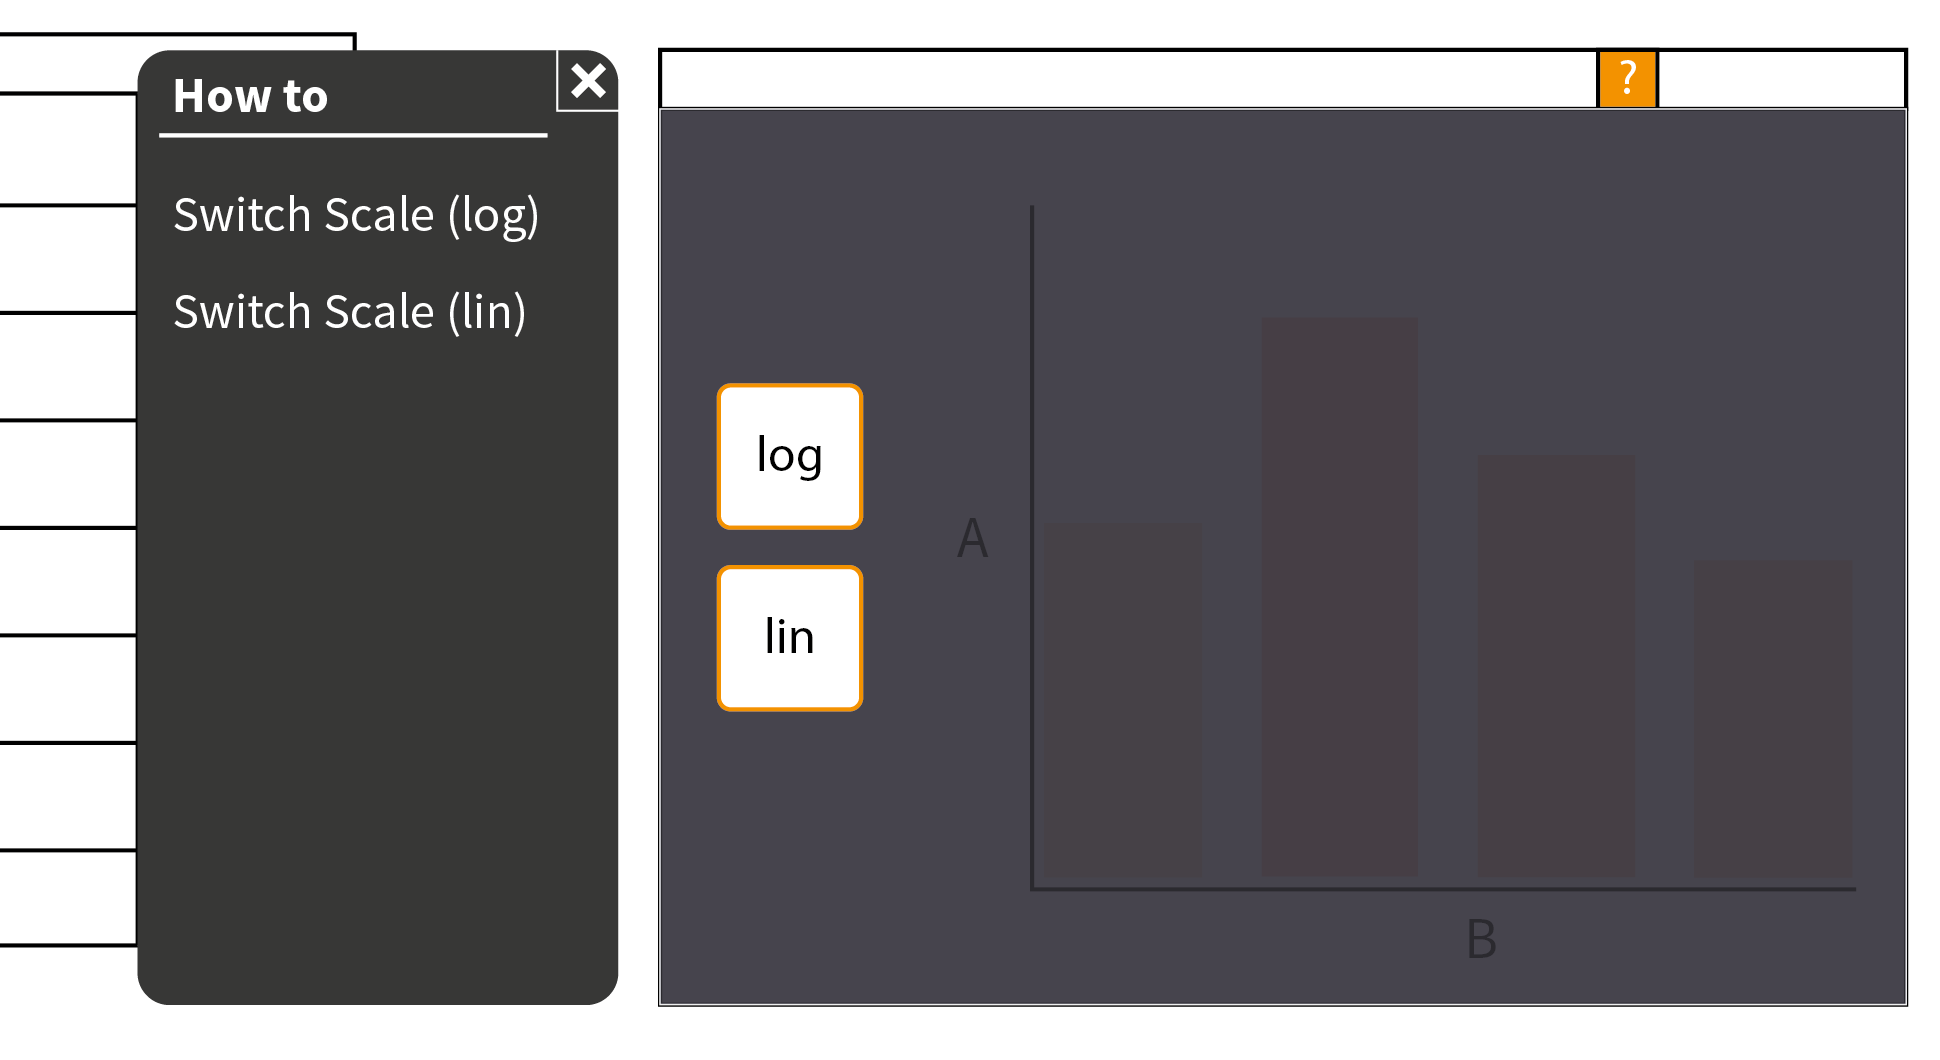
\includegraphics[width=0.5\textwidth]{images/konzeption-bedienung-step1.png}
   \caption{UI Mockup: Bedienung (Schritt~1)}
   \label{figure:bedienung-step1}
\end{figure}

Danach werden schrittweise mindestens drei Panels in der Komponente angezeigt (Abbildung~\ref{figure:bedienung-step2}). Der Inhalt der Panels ist in Abbildung~\ref{figure:bedienung-comic} zu sehen. Das erste Panel startet mit der ganzen Komponente, zoomt dann aber auf die relevanten UI Elemente. Panel~2 startet wiederum mit dem Inhalt von Panel~1, überblendet dann aber eine notwendige Operation. Das dritte Panel startet mit dem Inhalt aus Panel~1, zoomt aber auf eine Gesamtansicht wie anfangs hinaus, sodass der Benutzer den Unterschied sehen kann. Mit den Pfeilen kann zwischen verschiedenen Operationen gewechselt werden, die dieselbe Aktion ausführen. Sollte eine Aktion aus mehreren zusammenhängenden Operationen bestehen, wiederholen sich die Panels~1 und~2 dementsprechend. Falls mehrere gleichwertige Operationen eine Aktion ausführen, so können die Panels~1 und~2 gescrollt werden.

\begin{figure}[htbp]
   \centering
   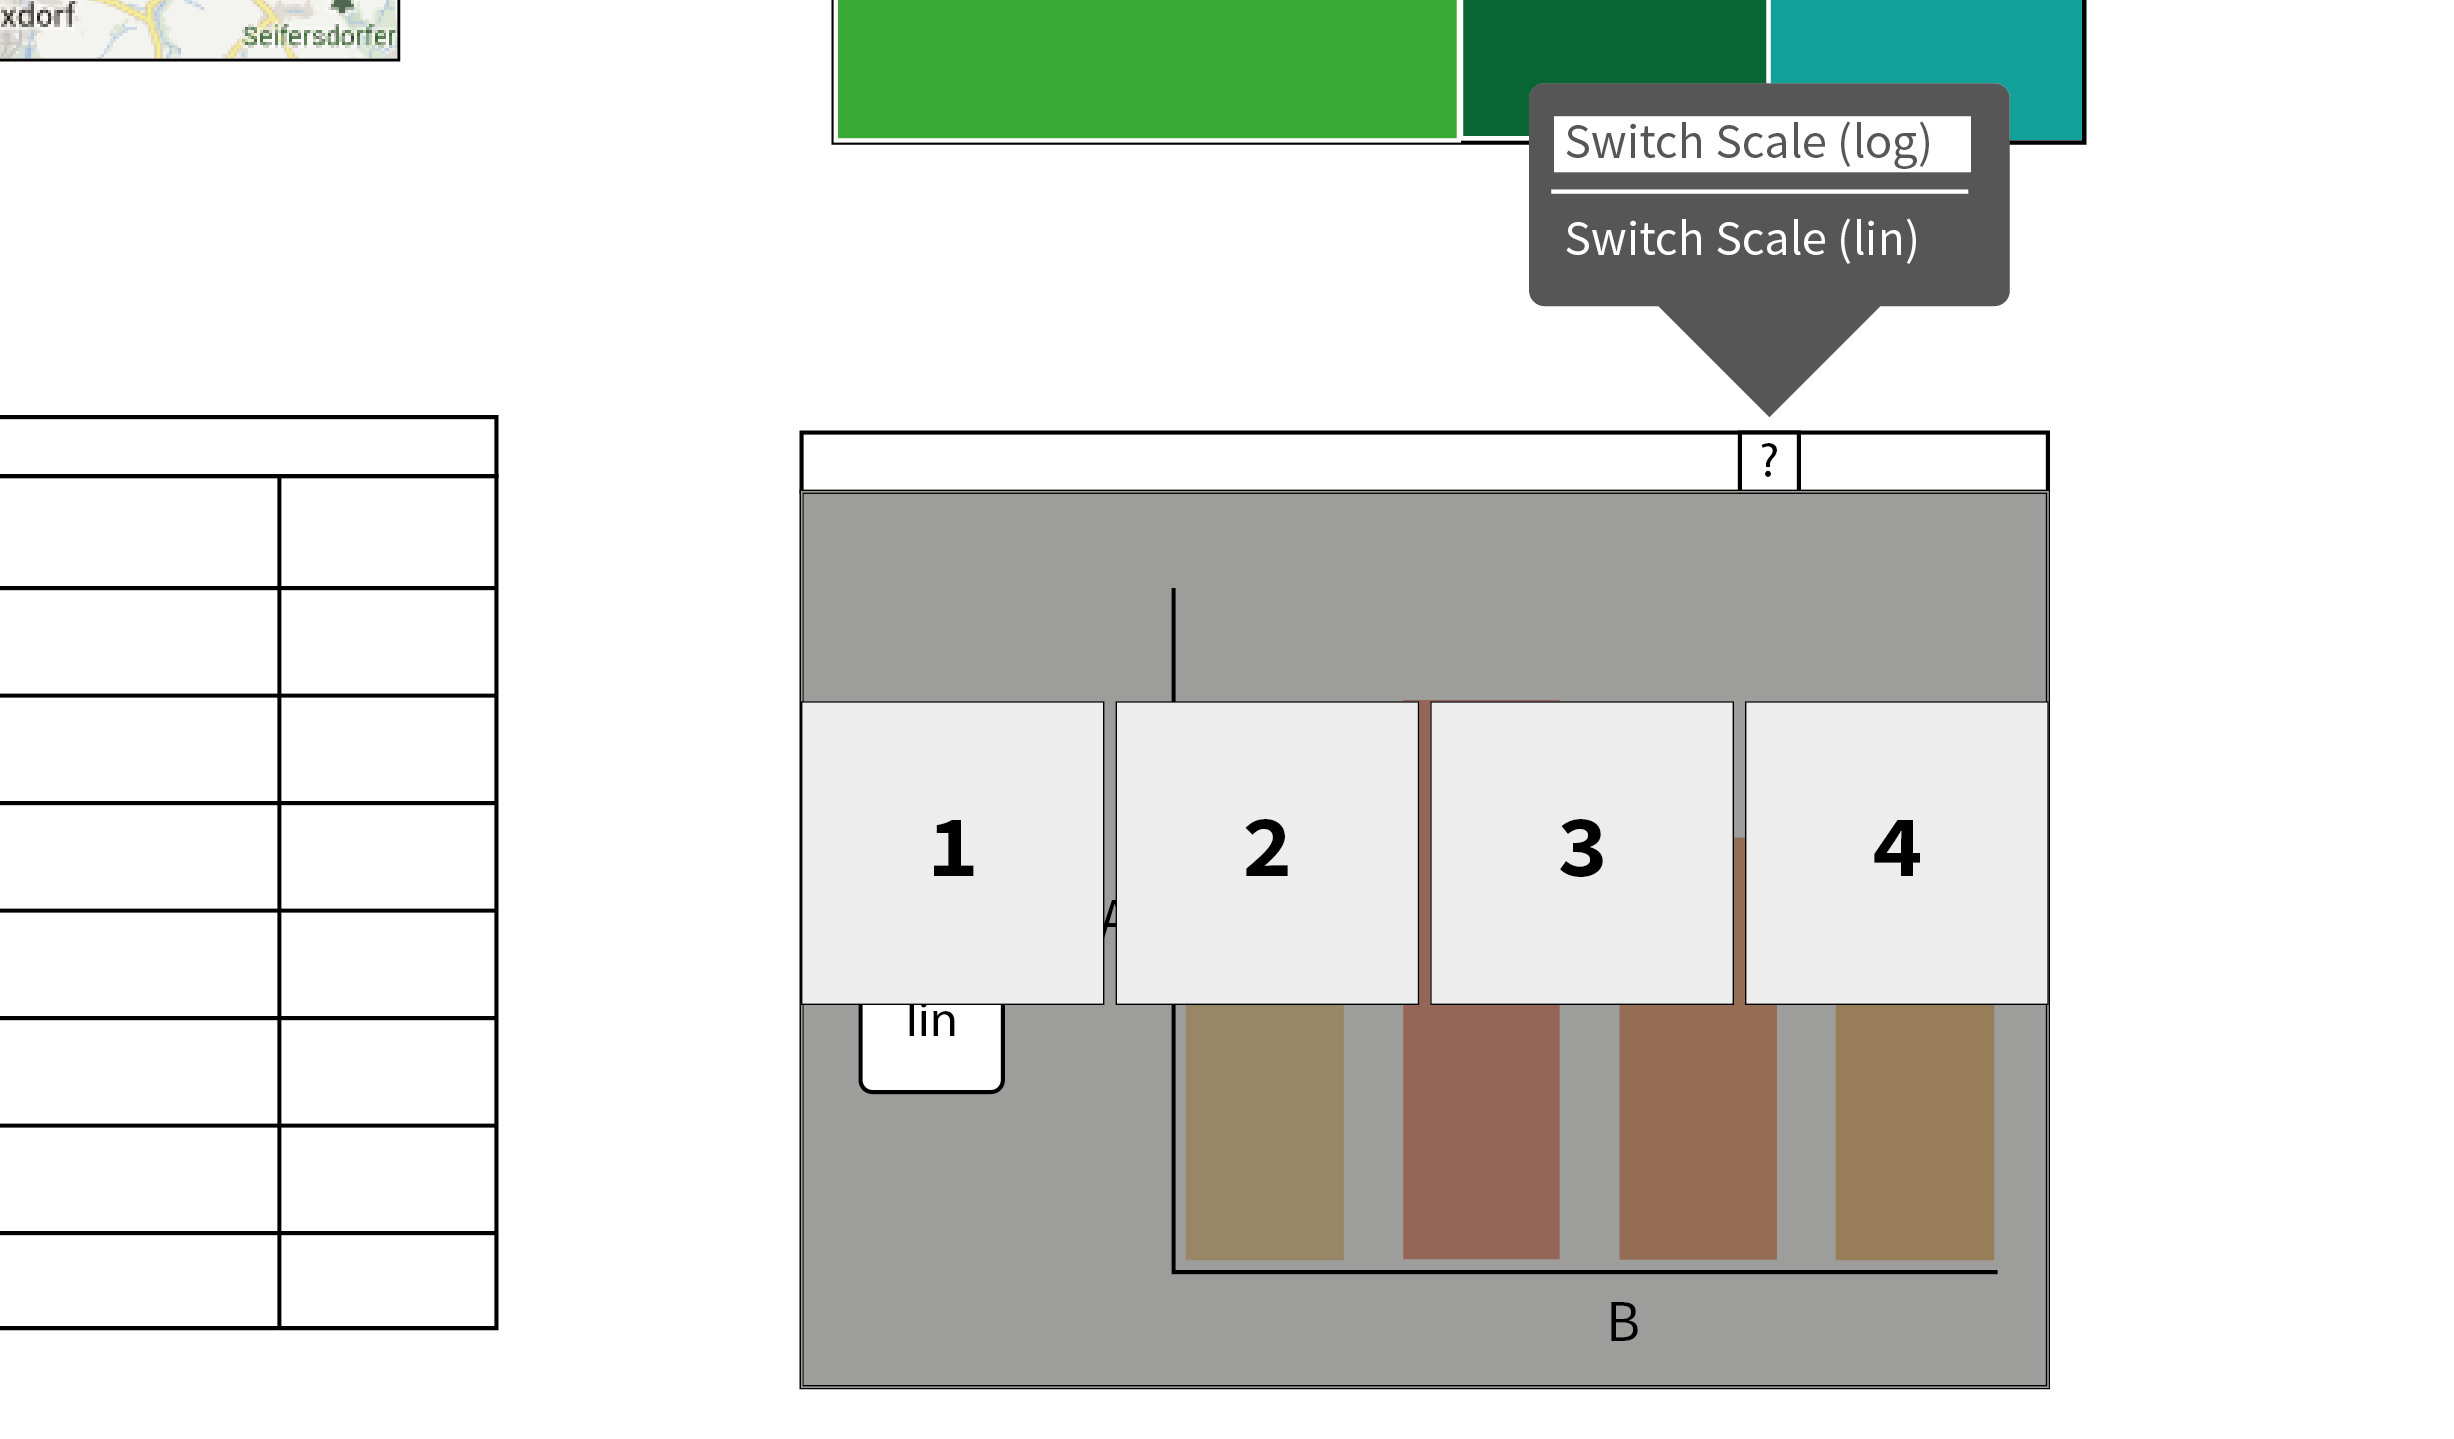
\includegraphics[width=0.5\textwidth]{images/konzeption-bedienung-step2.png}
   \caption{UI Mockup: Bedienung (Schritt~2)}
   \label{figure:bedienung-step2}
\end{figure}

\begin{figure}[htbp]
   \centering
   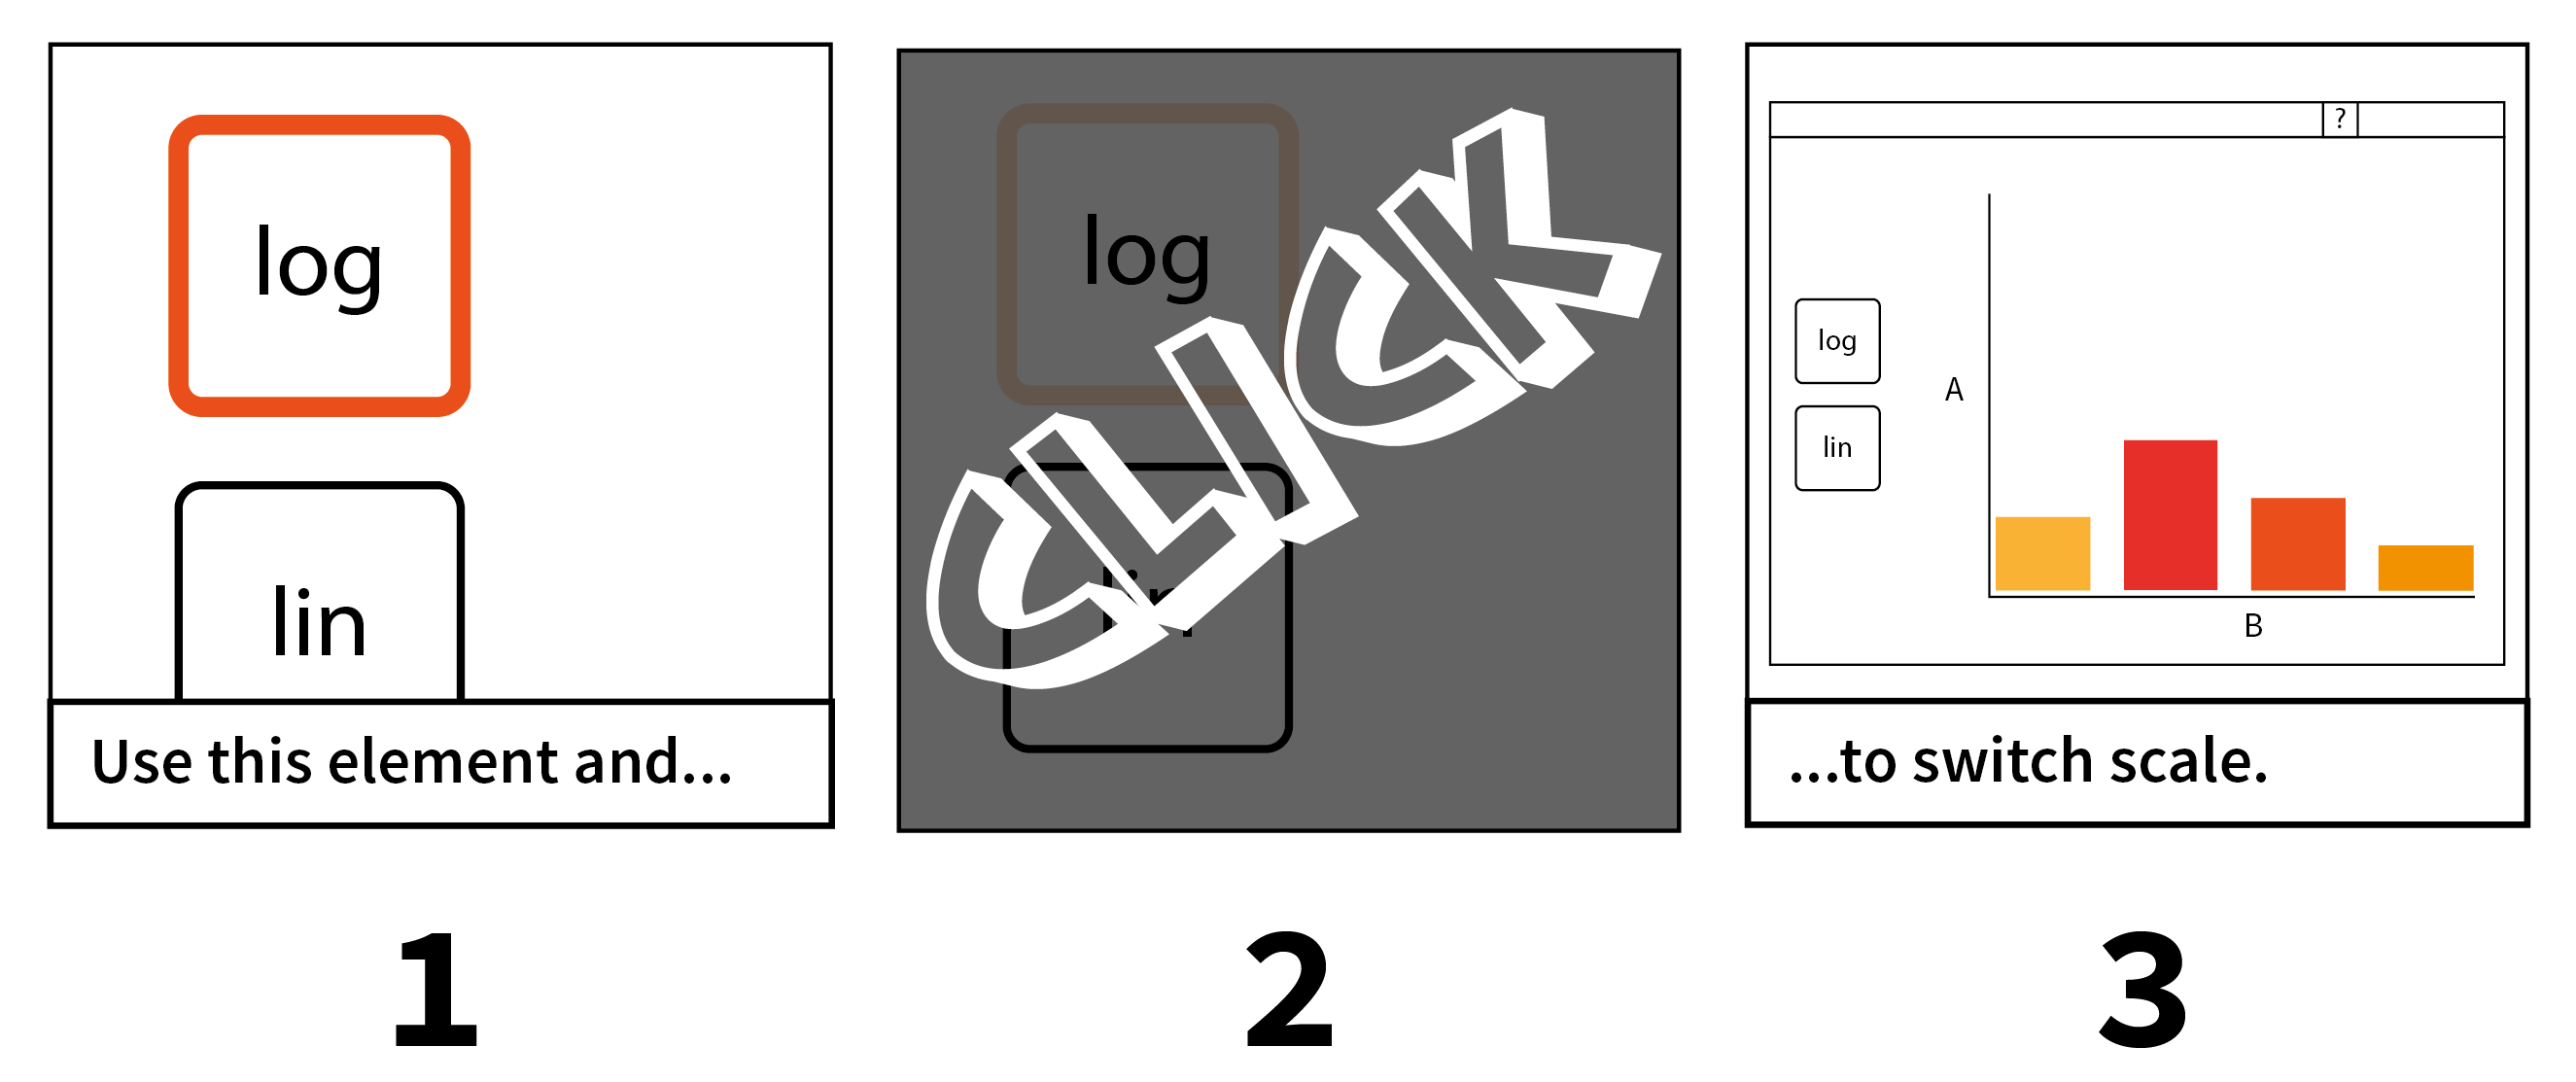
\includegraphics[width=0.75\textwidth]{images/konzeption-bedienung-comic.png}
   \caption{UI Mockup: Comic}
   \label{figure:bedienung-comic}
\end{figure}

Die Panels haben eine festgelegte Mindestgröße, um lesbar zu bleiben. Heer et al. \cite{Heer2008} verwenden in ihrer History, die ebenfalls Screenshots enthält, eine Seitenlänge von 120~Pixel. Falls die Komponente nicht breit genug sein sollte, um die nötige Anzahl von 120~Pixel großen Panels in einer Zeile anzuzeigen, wird die Bedienungshilfe in einem Fenster angezeigt. So können unterschiedliche, alternative Operationen immer gescrollt werden.

Die Texte in den Panels werden zur Laufzeit hinzugefügt, da so beispielsweise auf die Sprache des Nutzers reagiert werden kann. Ansonsten müsste der Hilfeservice für jede unterstützte Sprache ein eigenes Bild erzeugen. Die dafür notwendigen Informationen sind:

\begin{itemize}
	\item Panel~1: Welche Elemente beteiligt sind.
	\item Panel~2: Name der Operation.
	\item Panel~3: Name der Aktion.
\end{itemize}

Diese werden aber schon im Schritt davor (Abbildung~\ref{figure:bedienung-step2}) benötigt, müssen also sowieso bekannt sein.

\section{Feedback zu einer Komponente}
\label{section:konzeption:feedback}

Wie bei jeder Software können bei den Komponenten in VizBoard Fehler auftreten. Externe APIs, die sie benutzen, wie zum Beispiel von Facebook oder Twitter können sich ändern. Visualisierte Daten können Fehler in der Komponente verursachen, beispielsweise durch nicht überprüfte \texttt{null} Werte oder wenn sie ein unerwartetes Format haben. Ebenso ist es möglich, dass VizBoard selbst Bugs enthält. Schlimmstenfalls fallen diese Fehler erst dem Endnutzer auf, welcher sie dann melden können soll.

Für diejenigen, die sich mit dem Bug Report befassen müssen -- also Komponentenentwickler bzw. VizBoard-Betreiber -- sind möglichst genaue Angaben sehr wichtig. Welcher Browser wurde benutzt? Welche Version? Welches Betriebssystem? Was genau hat nicht funktioniert? Ist der Fehler reproduzierbar? Wenn ja, wie? Diese und andere Fragen müssen beantwortet werden, um letzten Endes die Fehlerquelle zu finden. Liegt es an der Komponente (z.\,B. wegen veralteten API Anfragen), an VizBoard (z.\,B. ein Bug im Event Broker) oder keinen der beiden (z.\,B. fehlerhafte Daten von der externen API)? Aus Sicht des Endnutzers \enquote{funktioniert es nicht}, da er keine Kenntnisse der Programmierung besitzt und deswegen keine sinnvollen Hypothesen aufstellen, überprüfen und Schlußfolgerungen ziehen kann. Deswegen sollte der Endnutzer einen möglichst ausführlichen Text verfassen, um das Problem zu beschreiben, und die Möglichkeit haben, die Komponente prinzipiell als gut oder schlecht zu bewerten. Letztere Funktion existiert bereits in VizBoard und wird in die Feedback UI integriert. Die anderen Informationen, wie eben beispielsweise die Browserversion, sollten automatisch gesammelt und mitgeschickt werden.

\subsection{User Interface und Interaktion}
\label{section:konzeption:feedback:ui}

Der Nutzer klickt auf einen Button in der Titelleiste, beschreibt sein Problem und sendet ab (Abbildung~\ref{figure:feedback}). Optional kann er außerdem eine Bewertung abgeben \cite{Voigt2013b}.

\begin{figure}[htbp]
   \centering
   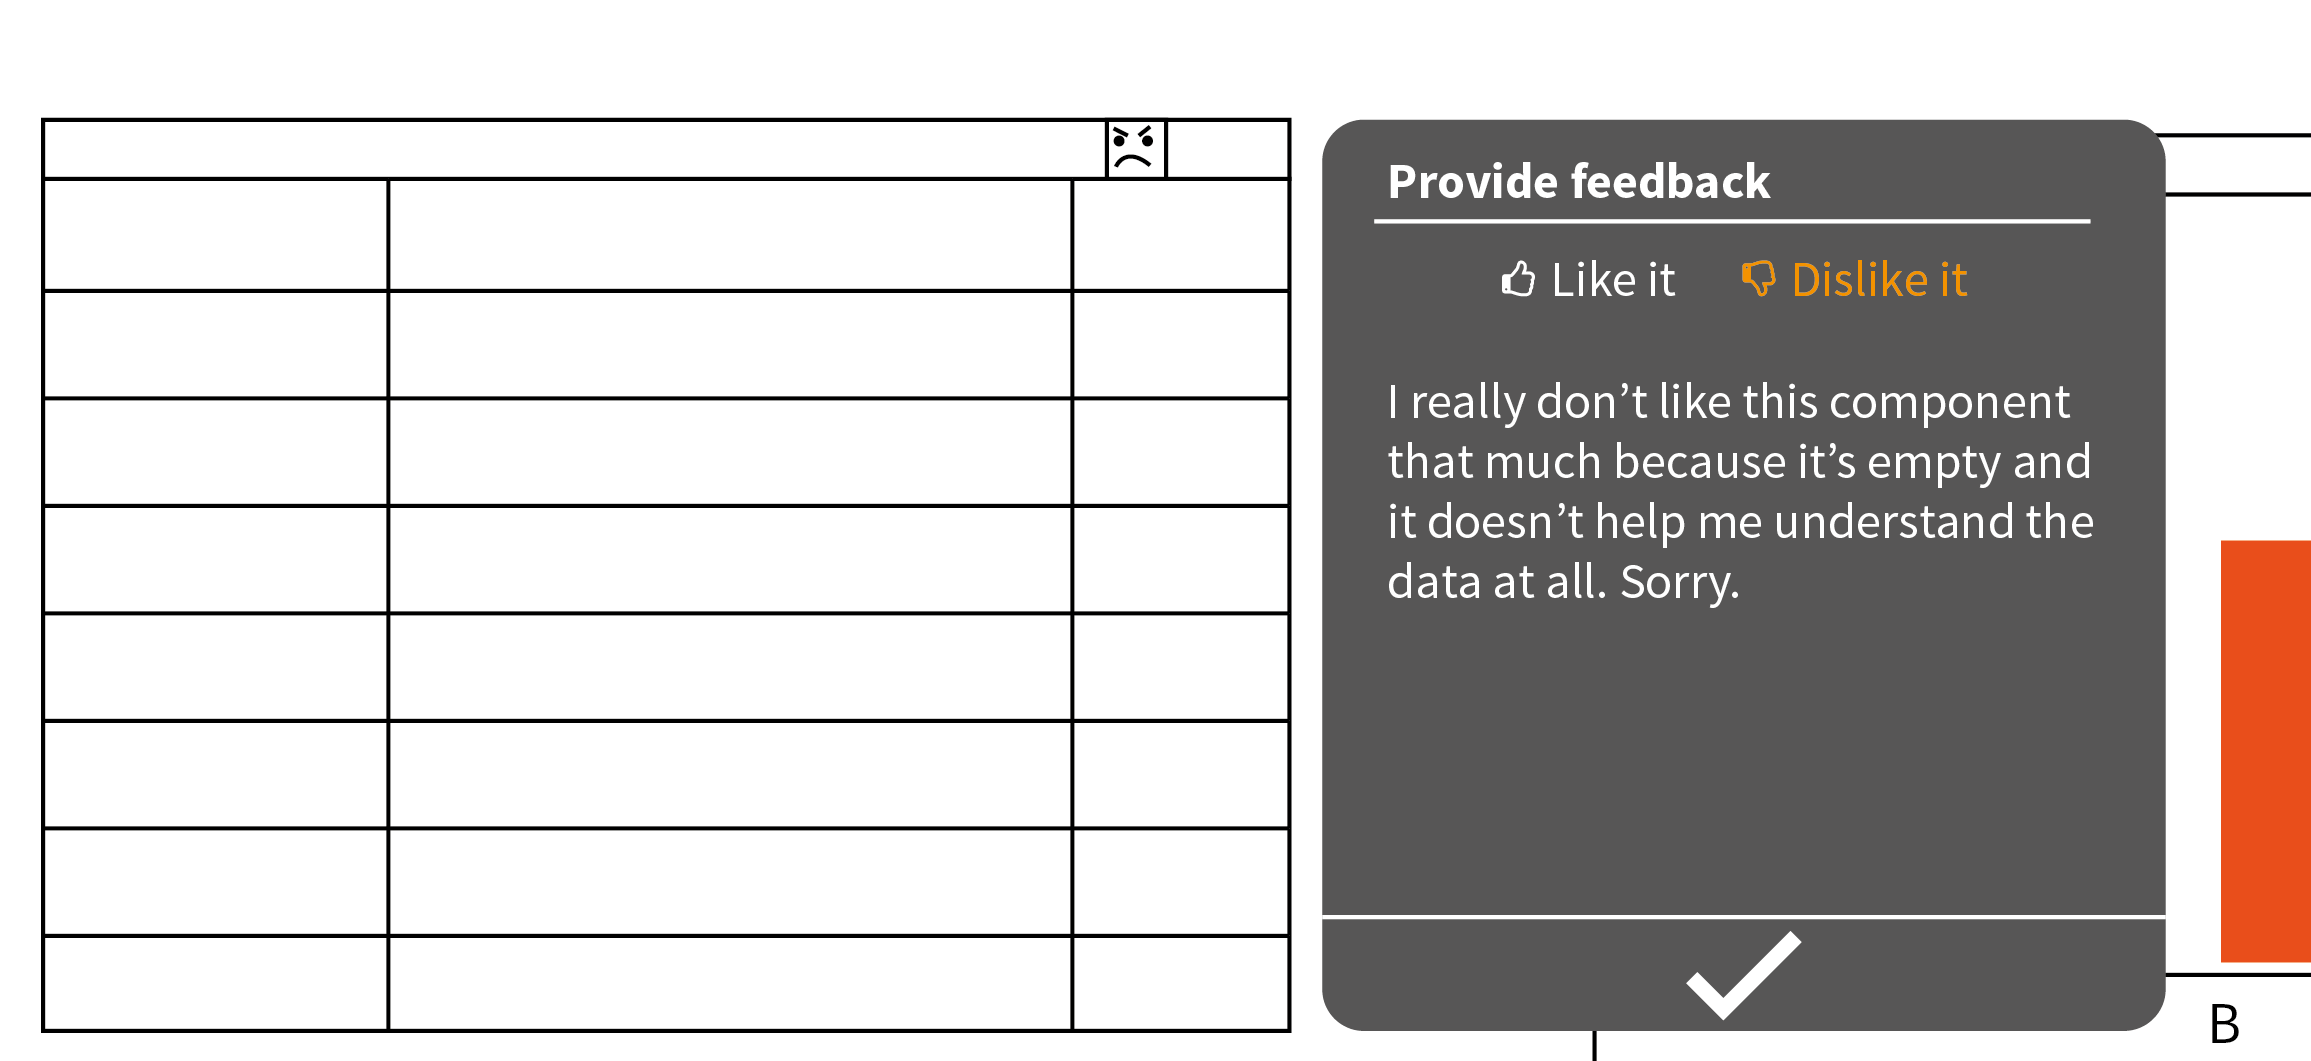
\includegraphics[width=0.5\textwidth]{images/konzeption-reporting.png}
   \caption{UI Mockup: Feedback-Funktion}
   \label{figure:feedback}
\end{figure}

\subsection{Backend}
\label{section:konzeption:feedback:backend}

% was kann man über javascript vom browser auslesen?
Informationen über den Browser befinden sich im DOM Objekt \texttt{window.navigator} und beinhalten unter anderem:

\begin{itemize}
	\item User Agent String, welcher Betriebssystem, Browser und deren Versionen enthält
	\item Sprache des Browsers
	\item Ob Cookies aktiviert sind
	\item Installierte Plugins, wie Java oder Flash
\end{itemize}

% was kann man über den context service bekommen?
% woher weiß man überhaupt, was es gibt? --> domänenspezifisches kontextmodell, ist also festgelegt.

Diese und andere notwendige Informationen können mit Javascript einfach ausgelesen werden. Noch mehr Informationen über den Nutzungskontext können über den Context Service (Abschnitt~\ref{section:standderforschung:grundlagen:cruise_vizboard}) bezogen werden. Dieser beinhaltet u.\,a. den Ort oder das Geschlecht des Nutzers.

% noch sagen dass es denkbar wäre, das direkt an ein support system anzubinden

Das Feedback des Nutzers wird ans Rating Repository gesendet und gespeichert. Die gesammelten Informationen aus dem Context Service über Nutzer, Browser und Anwendungskontext werden im RaRe referenziert. Das RaRe könnte aus der vom Nutzer abgegebenen Bewertung und Textklassifikation \cite{Sebastiani2002} in \enquote{positiv} oder \enquote{negativ} bestimmen, ob ein Ticket in einem Support System (wie z.\,B. OSTicket\footnote{\url{http://osticket.com/}}) des VizBoard-Betreibers erstellt werden soll. Die positiven Kommentare könnten beispielsweise für Testimonials auf der Startseite von VizBoard verwendet werden.

\section{Kommunikation zwischen Komponenten}
\label{section:konzeption:kommunikation}

Im kompositen Infomationsvisualisierungssystem VizBoard kommunizieren Komponenten miteinander, indem sie Nachrichten austauschen (Abschnitt~\ref{section:standderforschung:grundlagen:cruise_vizboard:kommunikationsmodell}). Dieser Vorgang ist für den Benutzer nicht sichtbar und kann für Verwirrung sorgen, wenn andere Komponenten auf Interaktionen reagieren, die dort nicht getätigt wurden. Dem wird beigekommen, indem 

\begin{enumerate}
	\item die Kommunikation zwischen Komponenten sichtbar gemacht wird und
	\item die Abhängigkeiten zwischen Komponenten wie bei der Bedienung (Abschnitt~\ref{section:konzeption:bedienung}) mit Comics erklärt werden.
\end{enumerate}

\subsection{User Interface und Interaktion}
\label{section:konzeption:kommunikation:ui}

Wie im vorigen Abschnitt erläutert, wird zuerst der Nachrichtenaustausch zwischen Komponenten sichtbar gemacht (Abbildung~\ref{figure:kommunikation-step1}). Dazu wird ein Pfeil vom Sender der Nachricht zum Empfänger animiert und gezeichnet, der in der Mitte ein Fragezeichen enthält. Das Fragezeichen wurde gewählt, da es konsistent mit dem Rest der Hilfe ist und ein Brief in der Nutzerstudie Assoziationen mit \enquote{Email} oder \enquote{in sozialen Netzwerken teilen} weckte. Sollten mehrere Empfänger vorhanden sein, existiert für jeden davon ein Fragezeichen. Die Kommunikationshilfe wird gleichzeitig mit der Bedienungshilfe (Abschnitt~\ref{section:konzeption:bedienung}) aufgerufen, solange wenig genug Komponenten im Mashup vorhanden sind (Abschnitt~\ref{section:konzeption:einleitung:nutzerstudie}). Ansonsten wird zusätzlich bei jeder Nachricht ein entsprechender Pfeil eingeblendet und nach kurzer Zeit (ca. 200--500~ms) wieder ausgeblendet.

\begin{figure}[htbp]
   \centering
   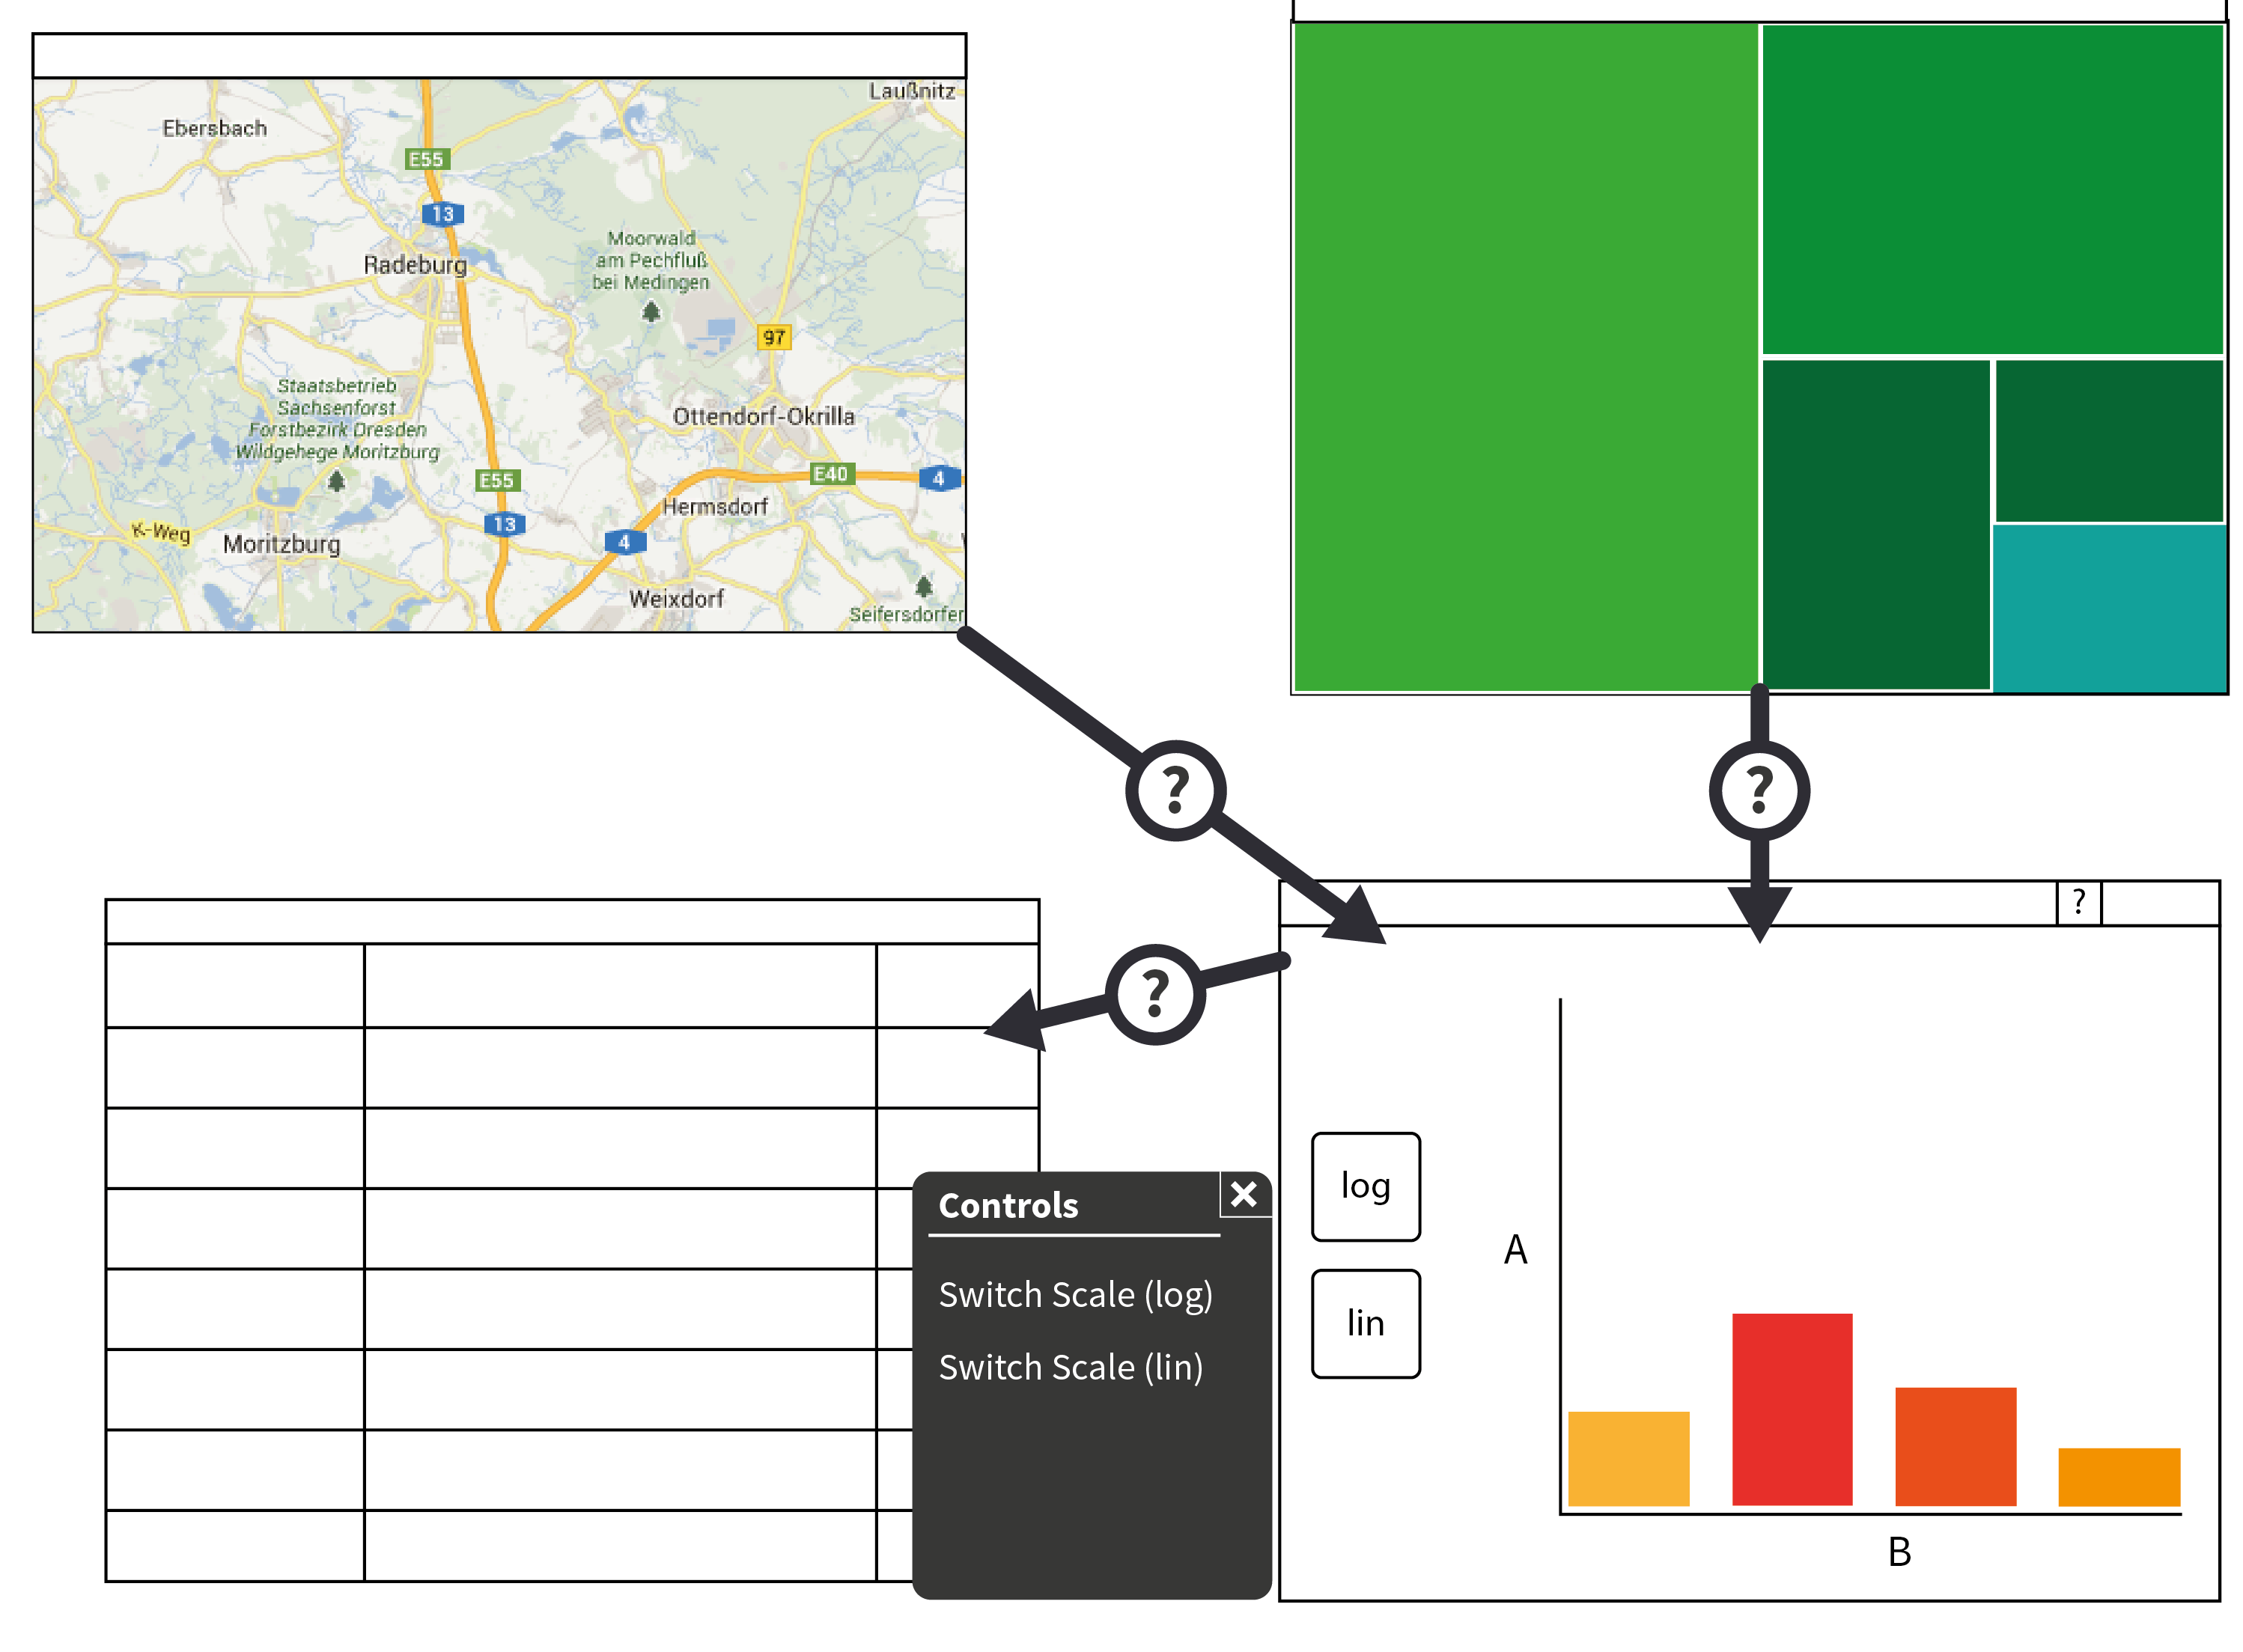
\includegraphics[width=0.5\textwidth]{images/konzeption-kommunikation-step1.png}
   \caption{UI Mockup: Kommunikationshilfe}
   \label{figure:kommunikation-step1}
\end{figure}

Wenn eine Akion ausgewählt wird, wird die Anzahl der gezeigten Pfeile entsprechend eingegrenzt (Abbildung~\ref{figure:kommunikation-step2}).

\begin{figure}[htbp]
   \centering
   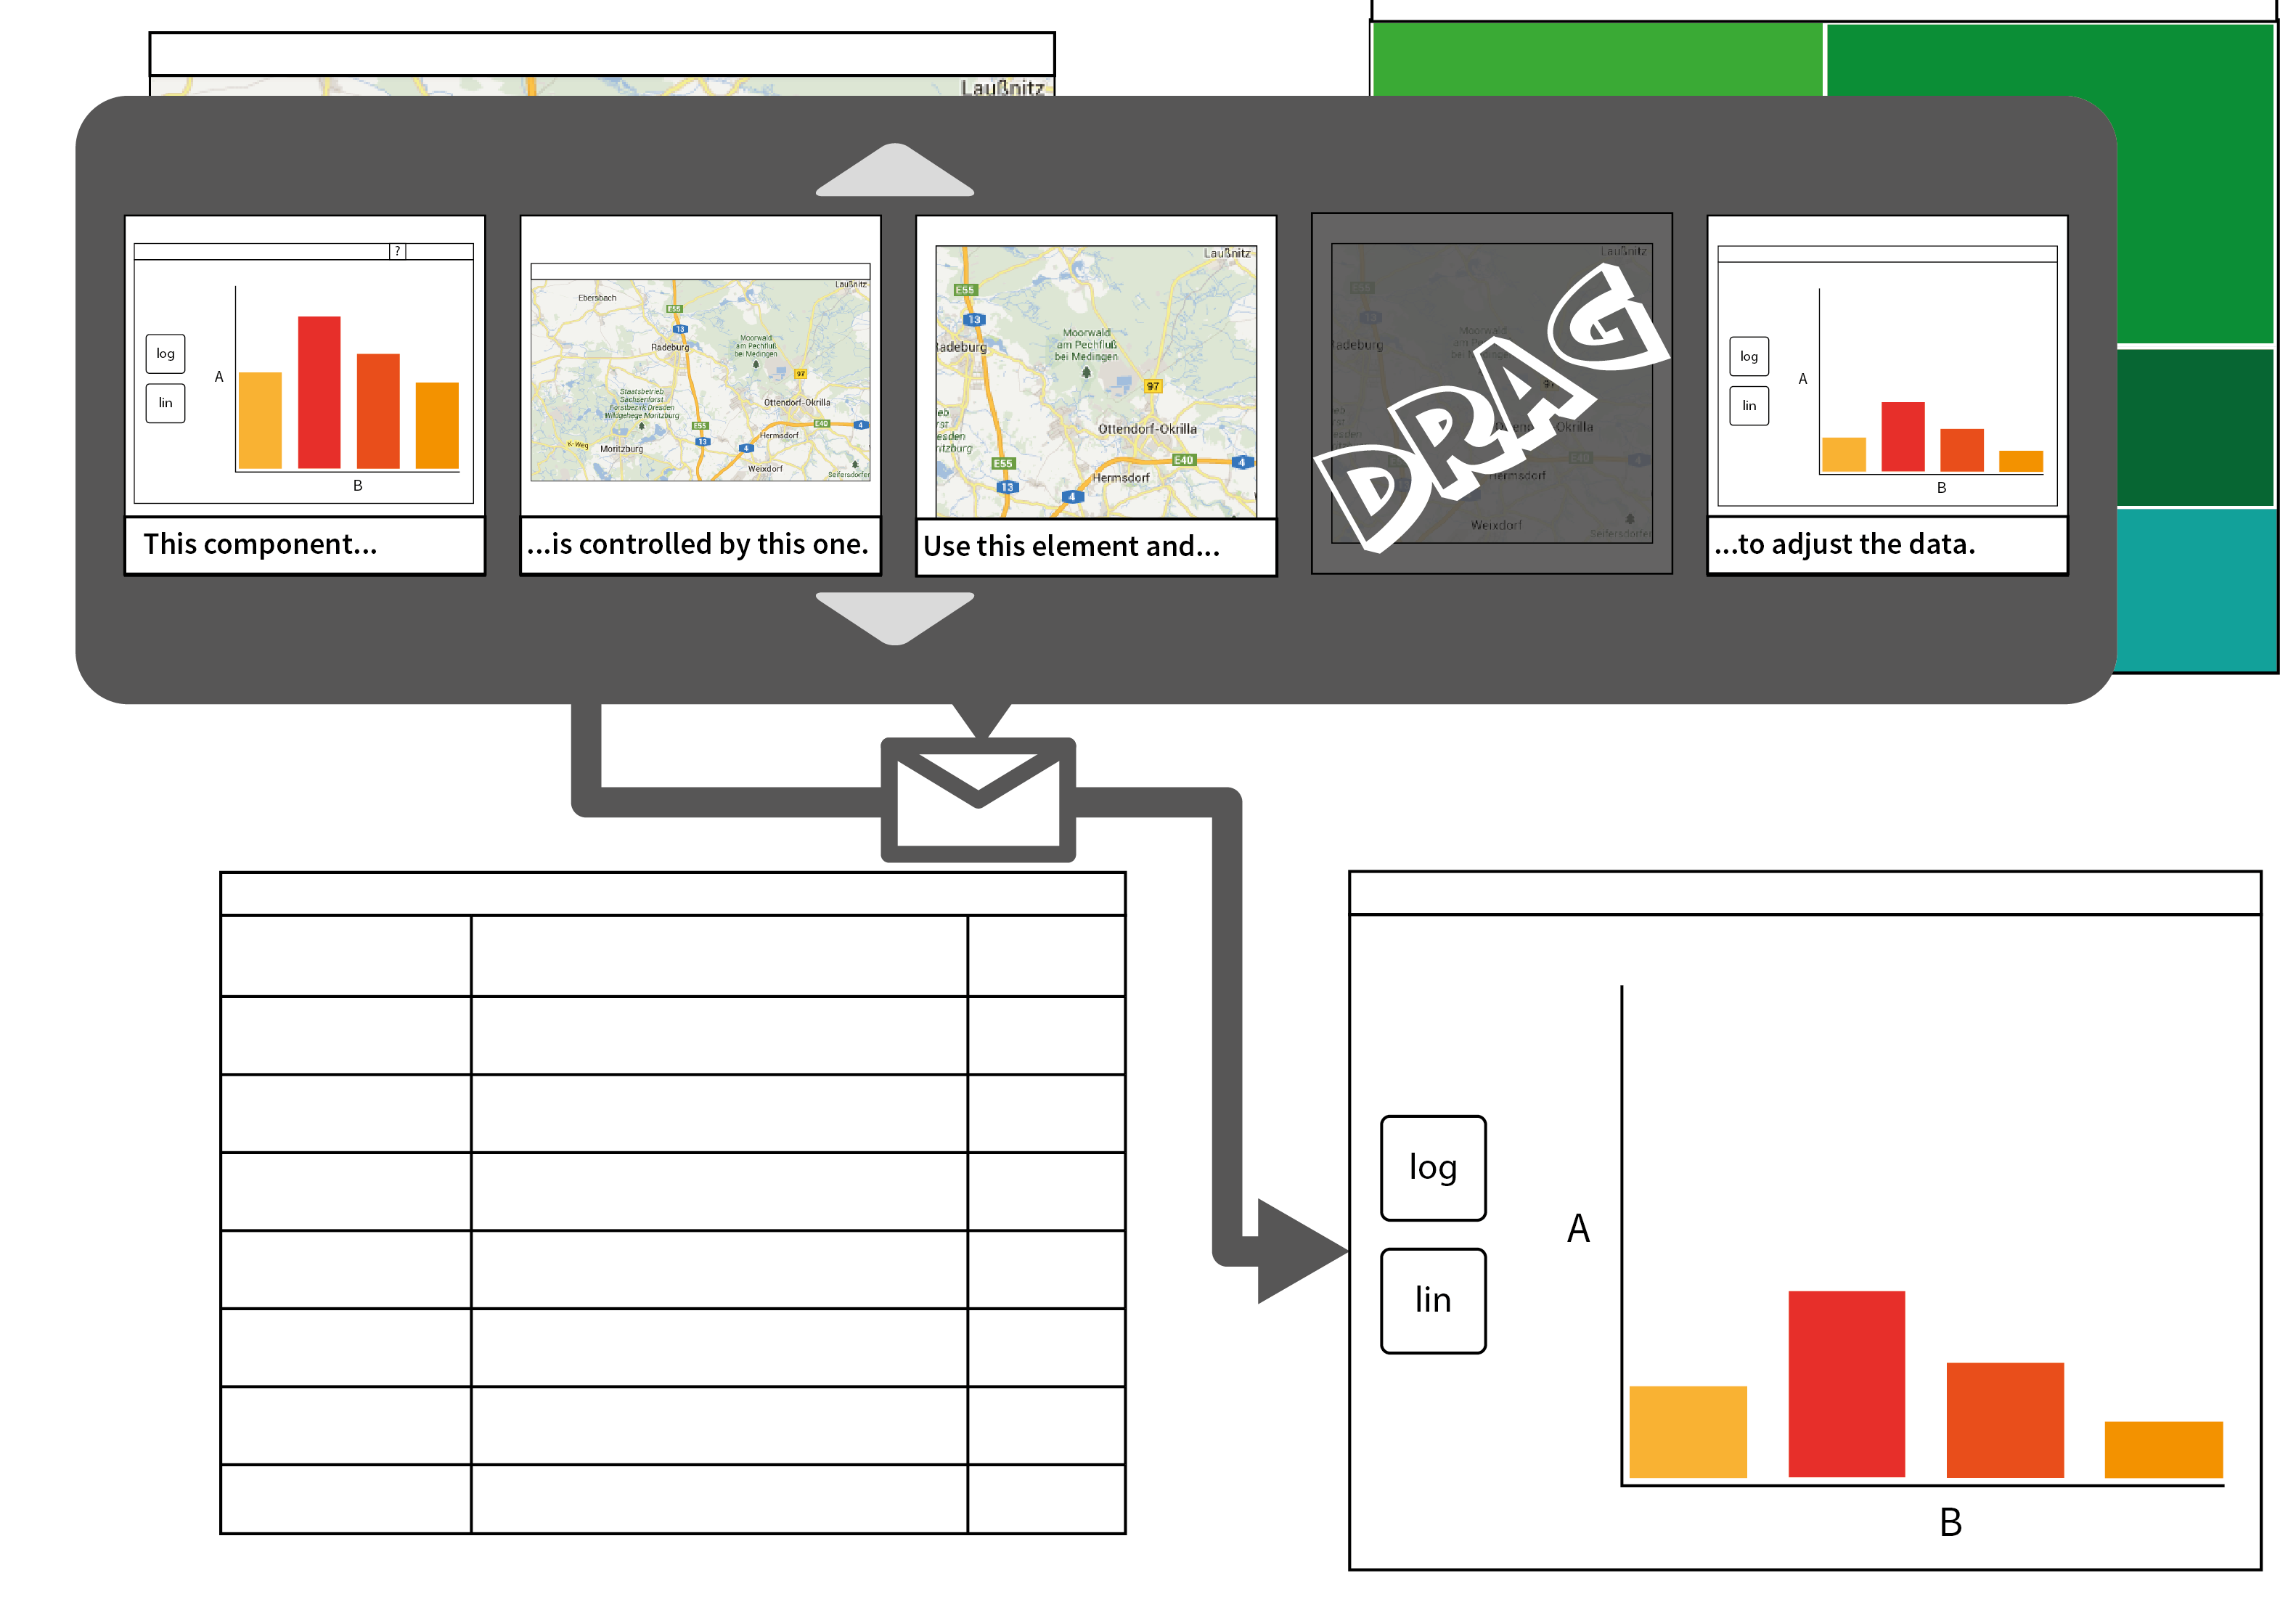
\includegraphics[width=0.5\textwidth]{images/konzeption-kommunikation-step2.png}
   \caption{UI Mockup: Kommunikationshilfe mit eingeschränkten Optionen}
   \label{figure:kommunikation-step2}
\end{figure}

Die Abhängigkeiten zwischen den beiden Komponenten werden erklärt, nachdem auf das Fragezeichen geklickt wurde (Abbildung~\ref{figure:kommunikation-step3}). Ein Fenster wird geöffnet, welches fast den gleichen Comic wie in Abschnitt~\ref{section:konzeption:bedienung} enthält. Der einzige Unterschied ist, dass anstatt einer VISO Operation eine VISO Aktion genannt wird. Auf diese Weise wird die Frage beantwortet, wie sich die angezeigten Komponenten beeinflussen und was Aktionen in anderen Komponenten bewirken.

\begin{figure}[htbp]
   \centering
   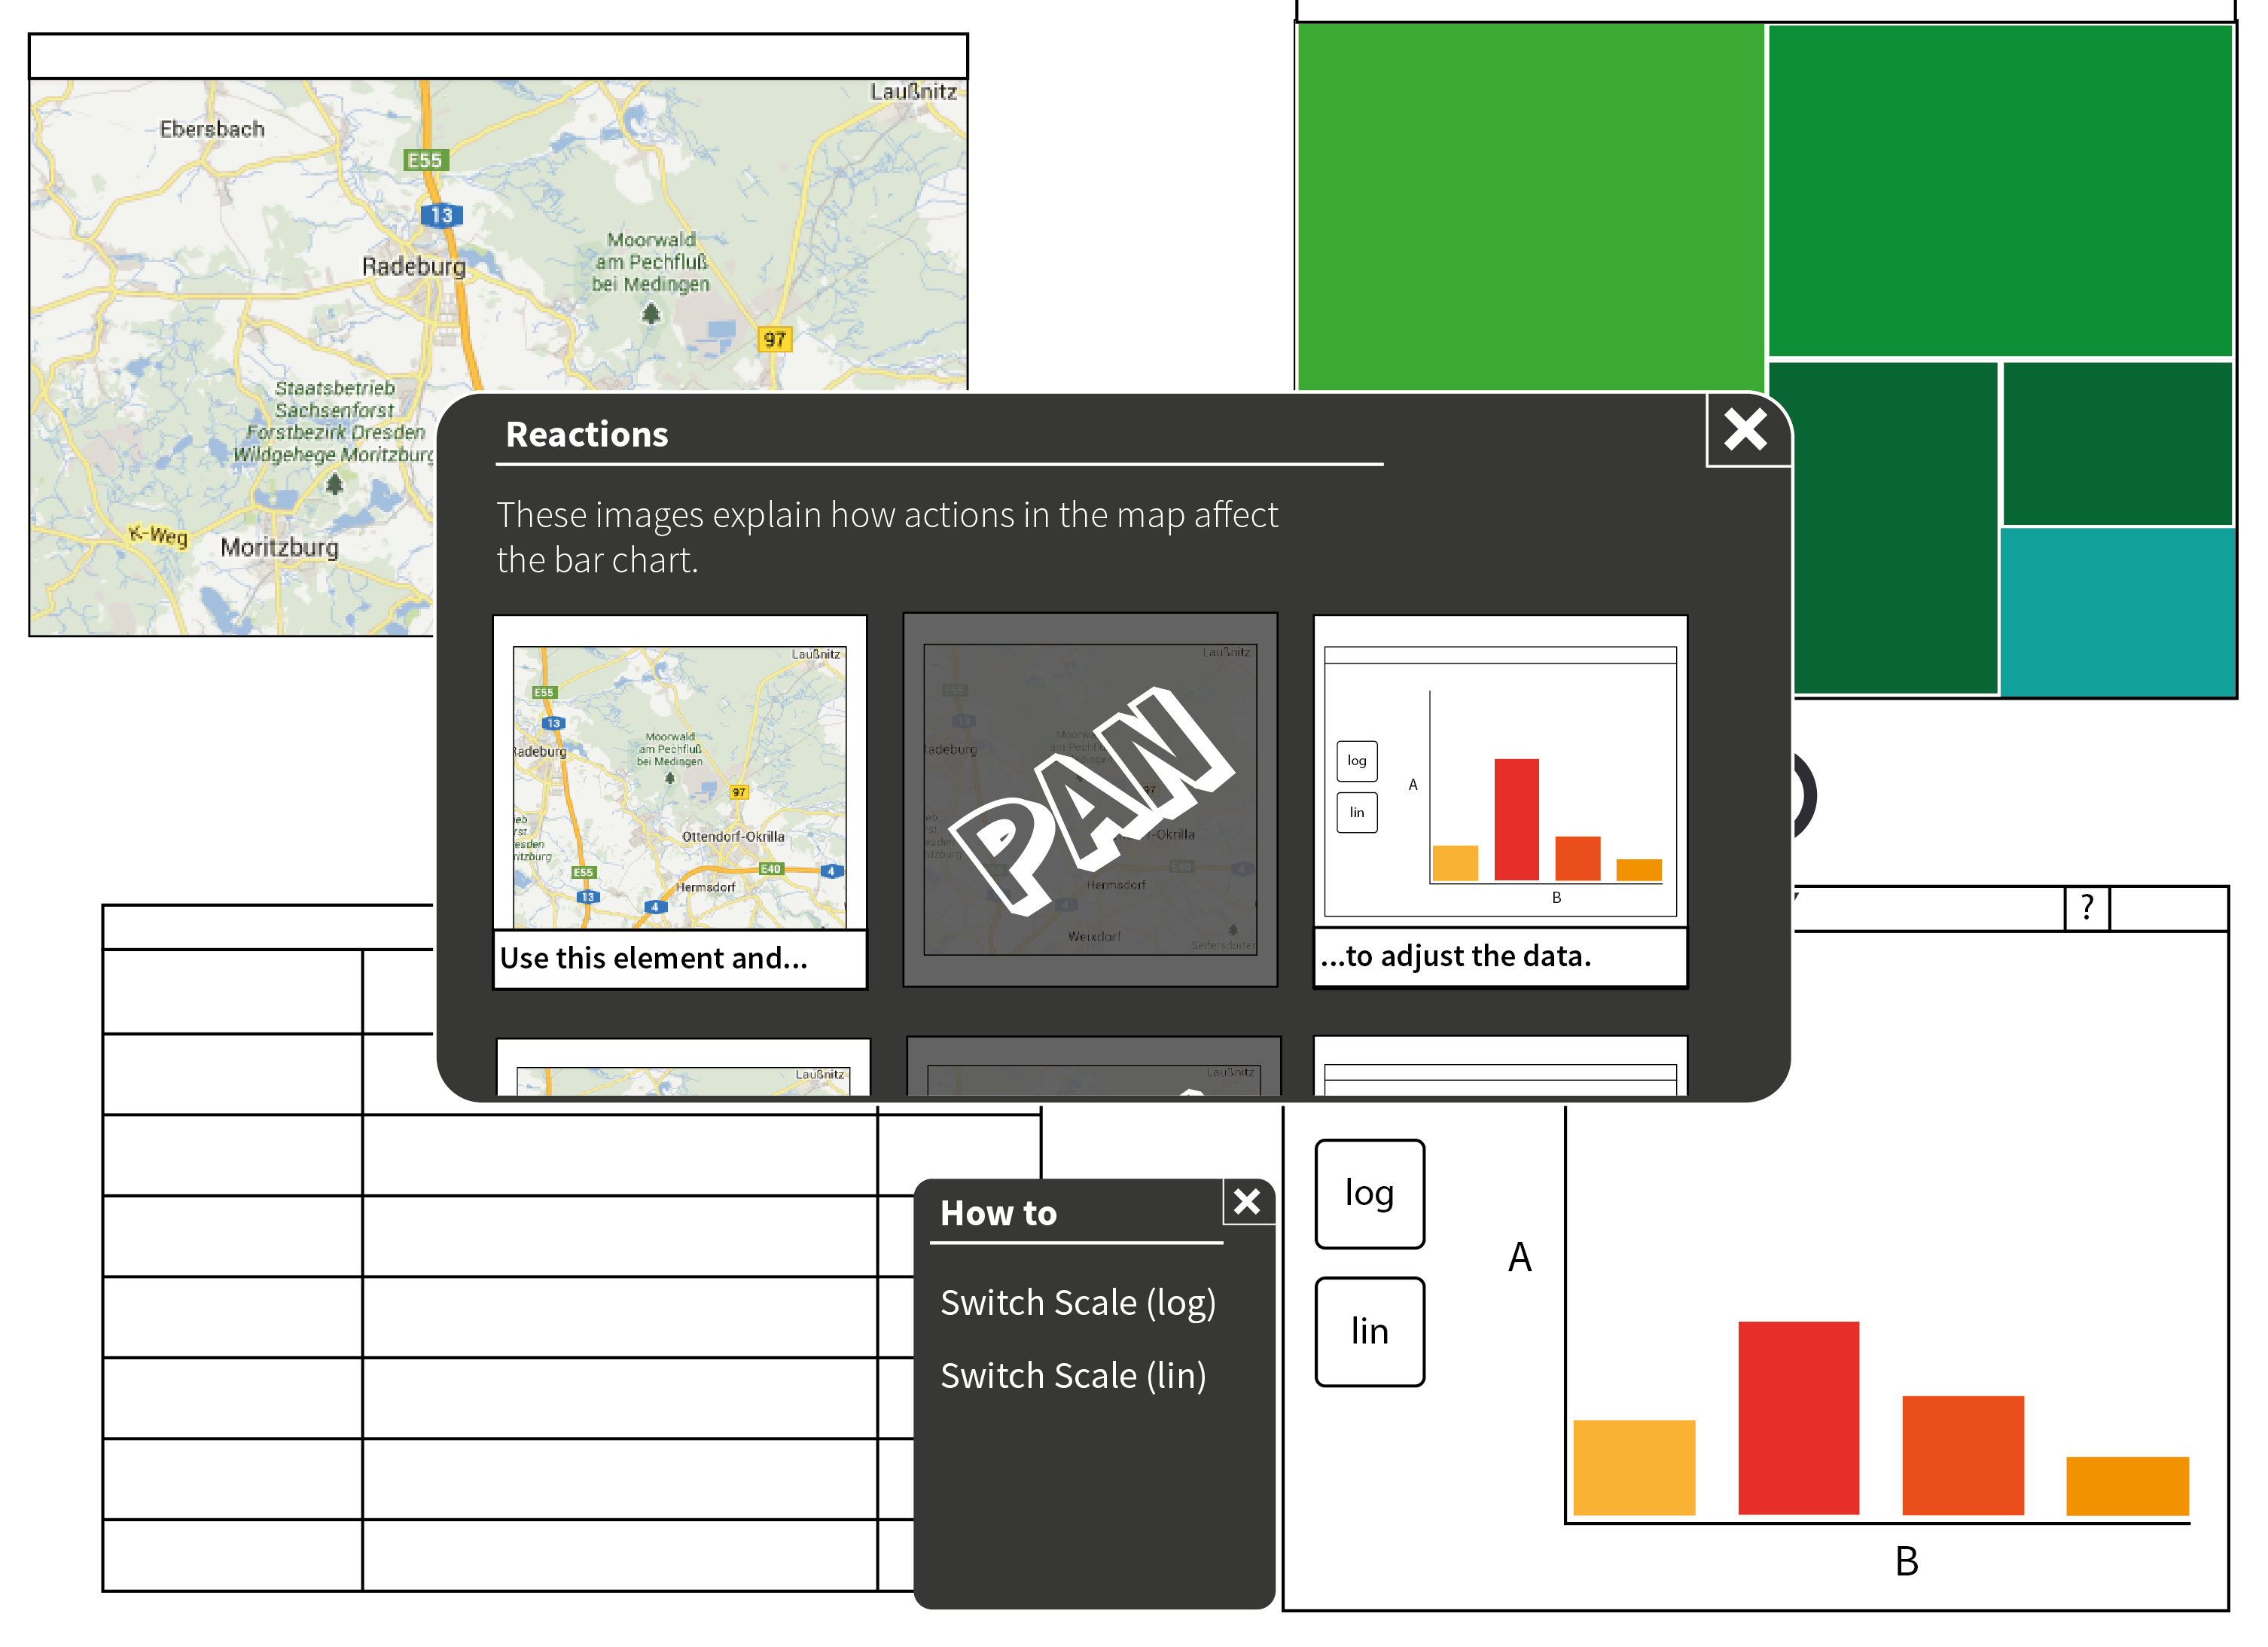
\includegraphics[width=0.5\textwidth]{images/konzeption-kommunikation-step3.png}
   \caption{UI Mockup: Comic erklärt Kommunikation. Verändern des Kartenausschnittes (Aktion: Panning, Operation: Drag) bewirkt ein Update im Balkendiagramm.}
   \label{figure:kommunikation-step3}
\end{figure}

\subsection{Backend}
\label{section:konzeption:kommunikation:backend}

Die Kommunikation zwischen Komponenten kann über den Event Broker (Abschnitt~\ref{section:standderforschung:grundlagen:cruise_vizboard}) nachvollzogen werden, da dieser zentraler Austauschpunkt für Nachrichten ist. Das Hilfesystem zeichnet Pfeile, wenn es vom Event Broker über Nachrichten informiert wird und die dynamische Kommunikationshilfe aktiviert ist.

Für die Generierung des Comics muss das Konzept der User Assistance für Bedienung (Abschnitt~\ref{section:konzeption:bedienung:api}) nur leicht erweitert werden. Da Komponenten mit Operationen auf Nachrichten reagieren (Abschnitt~\ref{section:standderforschung:grundlagen:cruise_vizboard:kommunikationsmodell}), muss für das Ergebnis einer Operation ebenfalls ein Screenshot erstellt werden. Diese sind jetzt schon in der Komponentenbeschreibung vorhanden und können während der Panel-Generierung einfach ausgeführt werden. Sollten die Operationen Parameter erwarten, muss der Komponentenentwickler Beispieldaten in die Komponentenbeschreibung einfügen.

Zu beachten ist allerdings, dass es Operationen geben kann, welche das User Interface der Komponente nicht verändern. Das Konzept der Hilfestellung mit Comics fußt darauf, dass ein sichtbarer Unterschied zwischen den Zuständen vor und nach einer Interaktion bzw. Operation besteht. Ist jener nicht vorhanden, ergibt der Comic keinen Sinn mehr. Deswegen muss dem Komponentenentwickler eine Möglichkeit gegeben werden, Operationen zu identifizieren, für die keine Hilfe generiert werden soll. Das kann am einfachsten durch ein optionales Attribut in der Komponentenbeschreibung umgesetzt werden.

\section{Verlinkung von unbekannten Konzepten}
\label{section:konzeption:verlinkung}

% einführung - warum brauchen wir verlinkung?

Ein Punkt, der in den verwandten Arbeiten (Abschnitt~\ref{section:standderforschung:verwandte_arbeiten}) kaum behandelt wurde, ist dass der Benutzer mehr Informationen über die visualisierten Daten benötigen könnte. Er könnte auf vollständig (\enquote{Was ist ein Säurezeiger\footnote{Eine Pflanze, die nur auf Böden mit einem bestimmten ph-Wert wachsen kann.}?}) oder teilweise (\enquote{Wie ist das BIP definiert\footnote{Der Gesamtwert aller Waren und Dienstleistungen, die innerhalb eines Jahres in einer Volkswirtschaft hergestellt wurden und dem Endverbrauch dienen.}?}) unbekannte Begriffe treffen. Um das Verständnis der Daten zu fördern, müssen diese erklärt werden, weswegen sie mit einer externen Wissensbasis verlinkt sein sollen. Zu erklärende Begriffe werden vermutlich hauptsächlich in Legenden von Visualisierungen zu finden sein, können aber auch in Freitexten oder in Interaktionselementen vorkommen.

\subsection{Markup und Backend}
\label{section:konzeption:verlinkung:backend}

Um zu erklärende Begriffe für das Hilfesystem auffindbar zu machen, zeichnet der Komponentenentwickler sie mit einer dafür vorgesehenen CSS Klasse aus: Eine Klasse für Legenden, eine für Freitext. Diese können entweder in der Komponentenbeschreibung angegeben und so selbst gewählt werden, oder sie werden vom Vizboard-Betreiber festgelegt. Hier wird die letzte Variante umgesetzt, weil sie dem Komponentenentwickler etwas Aufwand erspart und \enquote{Kollisionen} mit bereits vorhandenen Klassen erstens unwahrscheinlich sind und zweitens einfach behoben werden können (beispielsweise mit dem Präfix \texttt{my-}). Der zu erklärende Begriff ist dann der Textinhalt des Tags mit der entsprechenden Klasse. Bei Interaktionselementen sind die CSS Selektoren für die Bedienungshilfe (Abschnitt~\ref{section:konzeption:bedienung}) schon vorhanden und das Konzept wird in Form einer URI in die Komponentenbeschreibung eingefügt.

Auf diese Weise können die erklärungsbedürftigen Konzepte über CSS Selektoren gefunden werden. Allerdings stellt sich die Frage, wie das Hilfesystem die Beschreibung lesen kann. Die Konzepte sind im Falle von Freitext dynamisch, bei Legenden statisch, aber abhängig vom Datensatz und bei Interaktionselementen statisch in Abhängigkeit der Komponente. Es erscheint sinnvoll eine einheitliche Zugriffsschicht für Konzeptbeschreibungen zu etablieren. Dabei bietet sich im Fall von VizBoard das DaRe an, welches als einheitliche Zugriffsschicht auf Daten konzipiert ist. Bei anderen auf CRUISe aufbauenden Mashups sollte das CoRe diese Funktion übernehmen.

Das DaRe findet das Domain Assignment eigenständig, nachdem ein Datensatz hochgeladen wurde. Danach sollte eine Beschreibung aus der externen Wissensbasis abgerufen und gespeichert werden. Das hat den Nachteil, dass die Informationen zum Zeitpunkt der Anzeige möglicherweise nicht mehr aktuell sind. Da sich aber Beschreibungen zu Konzepten wie \enquote{logarithmische Skala} kaum ändern sollten und als Beispiel die DBpedia nur ein- bis zweimal pro Jahr ein Update bekommt\footnote{\url{http://blog.dbpedia.org/category/dataset-releases/} zeigt ein bis zwei Artikel im Jahr, abgerufen am 01.07.2013.}, sollte das kein Problem sein. Im Gegenzug ist das Hilfesystem unabhängig von der DBpedia verfügbar und schneller, da im Vergleich zum dynamischen Abruf der Beschreibung ein Netzwerk Round Trip eingespart wird.

Im Fall von Interaktionselementen parst das CoRe die Komponentenbeschreibung, nachdem eine Komponente hochgeladen wurde. Dabei extrahiert es die notwendigen Konzepte und schickt diese ans DaRe, welches die Beschreibungen dazu abruft und speichert.

\subsection{User Interface und Interaktion}

Bei Legenden und Freitext wird hinter die entsprechend markierten DOM Elemente (siehe Abschnitt~\ref{section:konzeption:verlinkung:backend}) ein Fragezeichen eingefügt, um eine Interaktionsmöglichkeit anzudeuten. Dieses kann angeklickt werden, woraufhin eine Sidebar mit einer kurzen Erklärung des Konzepts angezeigt wird (Abbildung~\ref{figure:verlinkung}), bei Interaktionselementen wird zusätzlich die Bedienungshilfe (Abschnitt~\ref{section:konzeption:bedienung}) angezeigt. Die Sidebar enthält auch einen Link, der zu einer Erklärung in einer externen Wissensbasis führt. Zur Erklärung des Konzepts gehört auf jeden Fall eine kurze Beschreibung, wie sie im ersten Absatz von Wikipedia-Artikeln gegeben ist und idealerweise ein Bild, falls vorhanden. Ist keine Beschreibung in der Sprache des Benutzers vorhanden, wird sie auf englisch angezeigt.

\begin{figure}[htbp]
   \centering
   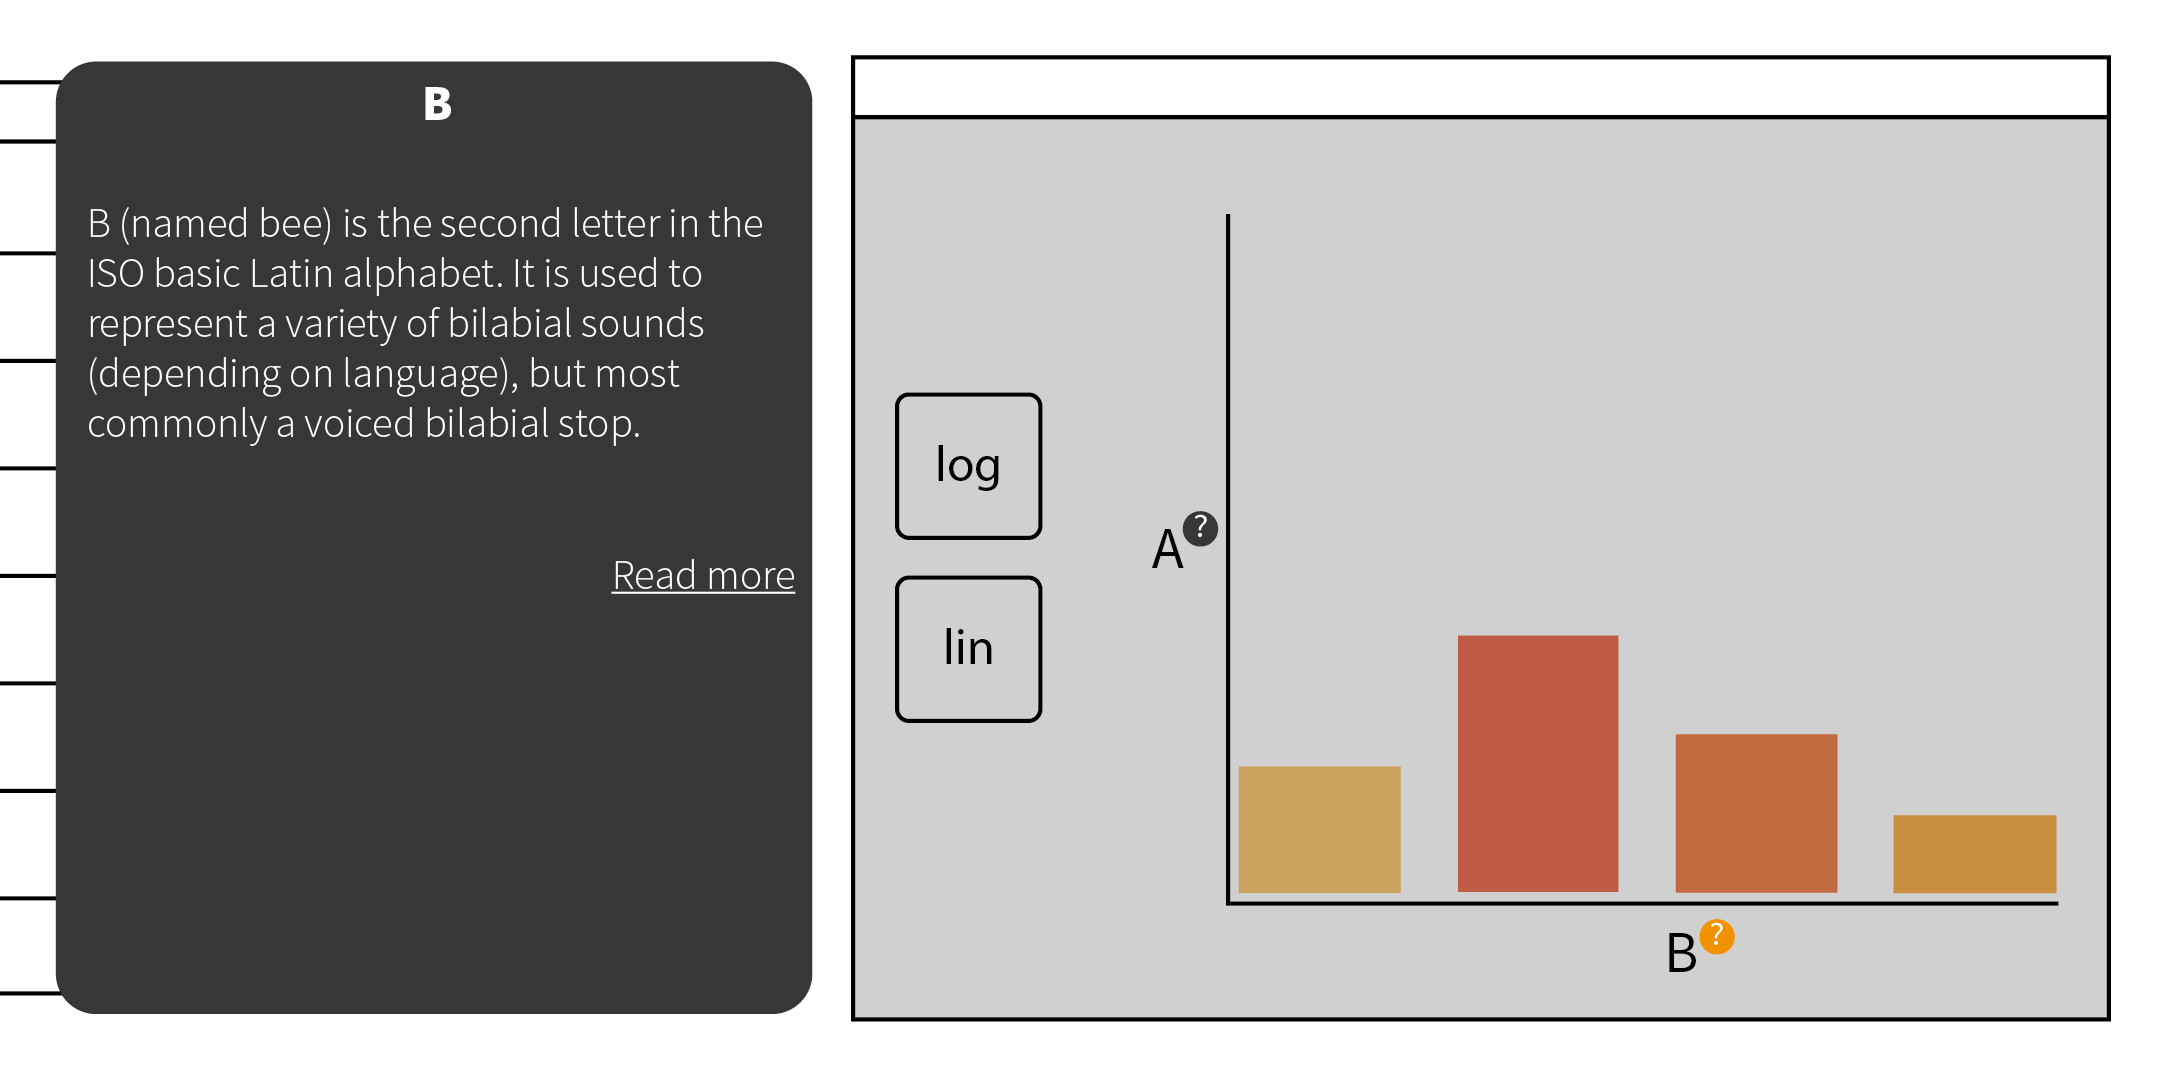
\includegraphics[width=0.5\textwidth]{images/konzeption-verlinkung.png}
   \caption{UI Mockup: Verlinkung von Legenden}
   \label{figure:verlinkung}
\end{figure}

Im Fall von Interaktionselementen wird bei \texttt{MouseOver} derselbe Hilfebutton eingeblendet (Abbildung~\ref{figure:verlinkung-bedienung}). Das hat den Grund, dass unbekannt ist, wie die Elemente angeordnet sind. Eine ständige Anzeige des Hilfebuttons könnte andere Elemente verdecken. Nachdem der Benutzer den Button gedrückt hat, werden falls vorhanden sowohl die Bedienungshilfe (Abschnitt~\ref{section:konzeption:bedienung}) als auch die ausgehende Kommunikation (Abschnitt~\ref{section:konzeption:kommunikation}) bei der betreffenden Aktion eingeblendet.

\begin{figure}[htbp]
   \centering
   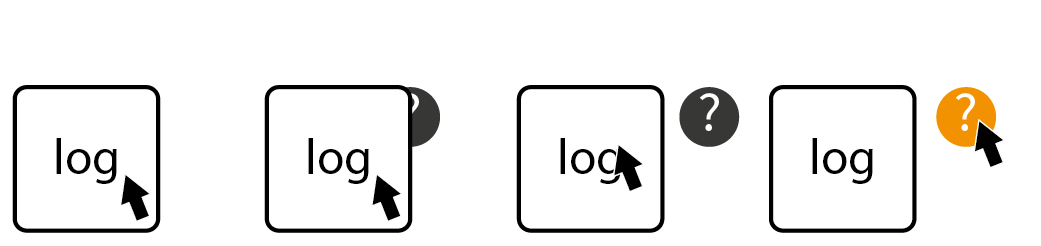
\includegraphics[width=0.5\textwidth]{images/konzeption-verlinkung-bedienung.png}
   \caption{UI Mockup: Verlinkung von Interaktionselementen}
   \label{figure:verlinkung-bedienung}
\end{figure}

Zwar wäre es wünschenswert, sowohl Legenden und Freitext als auch Interaktionselemente mit derselben UI kennzeichnen zu können. Das ist leider nicht ohne weiteres möglich. Würden Legenden und Freitext die UI der Interaktionselemente verwenden, wäre die Hilfefunktion nicht sichtbar. Wäre es andersherum, müsste der DOM auf nicht-triviale Weise manipuliert werden (Einfügen von eigenen Elternknoten usw.), was unerwünschte Auswirkungen auf CSS Selektoren des Entwicklers haben könnte.

\section{Kommentare in Visualisierungen}
\label{section:konzeption:kommentare}

% allgemeines zu kommentaren. woraus bestehen sie, was müssen sie können.

Kommentare waren in den verwandten Arbeiten (Abschnitt~\ref{section:standderforschung:verwandte_arbeiten}) eine populäre Variante, um das Verständnis der Daten zu fördern. Mit Hilfe von Kommentaren können Endnutzer andere auf beobachtete Fakten der Daten wie Ausreisser oder Trends hinweisen und so zum Verständnis beitragen. Der Begriff \enquote{Kommentartext} referenziert hier den Text, welcher von Benutzern geschrieben wird, und \enquote{Annotation} die Markierung in der Visualisierung. Ein \enquote{Kommentar} ist die Kombination aus beliebigen Annotationen und einem Kommentartext.

% wie können kommentare umgesetzt werden? dev vs us! warum machen wir es so wie geplant?

Prinzipiell gibt es zwei Varianten, wie Kommentare in einer InfoVis-Komponente umgesetzt werden können. In der ersten kümmert sich die Komponente darum, wie und wann sie Kommentare lädt und anzeigt. Der Vorteil daran ist, dass die Handhabung von Kommentaren speziell auf jede Komponente angepasst wird. Allerdings kann so kein \emph{einheitliches} Look \& Feel gewährleistet werden. Zwar könnten Designrichtlinien Aussehen und Interaktionen vorschreiben, sie sind aber zwecklos wenn der Komponentenentwickler sie nicht einhält. Außerdem erhöht diese Variante den Entwicklungsaufwand der Komponente stark (\emph{Minimalität}).

In der zweiten Variante ist es Aufgabe des Hilfesystems, Kommentare zu verwalten und anzuzeigen. Die vorhin genannten Nachteile werden hier zu Vorteilen: Einheitliches Look \& Feel wird sichergestellt und der Komponentenentwickler hat keinen zusätzlichen Entwicklungsaufwand. Allerdings hat das Hilfesystem auf Grund des \enquote{Black Box} Prinzips keinen Zugriff auf die in der Komponente verwendeten Daten. Aus demselben Grund kommt hinzu, dass das User Interface für Kommentare sich verschiedenen Interaktionen der Komponente wie z.\,B. scrollen, Tab wechseln, zoomen etc. anpassen muss, ohne darüber informiert zu werden. Im folgenden wird erläutert, wie diese Nachteile umgangen werden können.

\subsection{Features}
\label{section:konzeption:kommentare:features}

% ### funktionen eines kommentars

In diesem Abschnitt wird diskutiert, welche Funktionen das Kommentarsystem zur Verfügung stellen soll.

\subsubsection{URL einfügen}

Es ist wahrscheinlich, dass Benutzer zur Erklärung der Daten bzw. Visualisierung auf externe Quellen verweisen müssen. Da VizBoard ohnehin webbasiert ist, eignen sich Links in Form von URLs dafür sehr gut.

\subsubsection{Kommentar referenzieren}

Um Diskussionen und Konversationen zur Visualisierung zu fördern, müssen Kommentare einander referenzieren können \cite{Heer2007}. So wird es Benutzern erleichtert, zusammen eine Erklärung für Ausreisser oder Trends zu finden. 

\subsubsection{Voting}

Erfahrungsgemäß tragen nicht alle Kommentare gleich viel zur Diskussion bei. Man denke dabei an Hinweise auf Tippfehler oder das berüchtigte \enquote{Erster!}. Deswegen ist es notwendig, dass Benutzer Kommentare anderer bewerten können.

\subsubsection{Ranking}

Da Diskussionen und Konversationen nicht durch das User Interface eingeschränkt werden sollen, ist es nötig, Kommentare nach Datum sortieren zu können. So kann der Gesprächsverlauf nachvollzogen werden. Wenn Benutzer aber nicht an der Konversation teilnehmen, sondern schnell eine Antwort auf ihre Fragen haben wollen, bietet es sich an, nach Bewertung sortieren zu können.

\subsubsection{Kommentar editieren}

Den eigenen Kommentar editieren zu können, ist aus verschiedenen Gründen wichtig, z.\,B. wenn der Benutzer Tippfehler ausbessern oder ein paar Absätze zur Lesbarkeit einfügen will. Wichtig ist für andere, dass dies transparent geschieht und die Diskussion nachvollziehbar bleibt. Es gibt verschiedene Lösungsmöglichkeiten:

\begin{itemize}
	\item Der Kommentar kann nicht editiert werden. So bleibt alles perfekt nachvollziehbar, aber der Benutzer kann nichts ausbessern.
	\item Der Kommentar kann nur für $x$ Minuten editiert werden, danach ist er gesperrt. Diese Variante erlaubt immerhin noch Tippfehler auszubessern, aber der Benutzer kann beispielsweise nicht nach einer Stunde eine Quelle einfügen.
	\item Der Kommentar kann beliebig editiert werden. Diese Variante ist aus Nutzersicht am Besten, aber sie muss anderen gegenüber transparent gemacht werden. Es muss sichtbar sein, dass ein Kommentar editiert wurde und wann. Im Idealfall würde auch die Originalversion eines referenzierten Kommentars mit abgespeichert, sodass diese später eingeblendet werden kann.
\end{itemize}

\subsubsection{Kommentar löschen}

Gründe, um einen Kommentar zu löschen, beinhalten unter anderem Beschimpfungen oder mangelnde Aktualität, etwa wenn eine zitierte Studie widerlegt wurde. Wie beim Editieren von Kommentaren ist es hier notwendig, dass der Gesprächsverlauf nachvollziehbar bleibt. Die Lösungsansätze beinhalten:

\begin{itemize}
	\item Kommentare können nicht gelöscht werden. Das könnte Benutzer davon abhalten, Kommentare zu schreiben, was auch nicht Sinn der Sache ist.
	\item Kommentare können gelöscht werden, solange keine Referenz darauf besteht. So kann ein Diskussionsverlauf konsistent bleiben, allerdings ist dieser Weg aus Nutzersicht schwer verständlich.
	\item Kommentare können beliebig gelöscht werden. Diese Variante weckt keine Ängste, den eigenen Kommentar nicht mehr löschen zu können. Es muss aber etwas mit den Referenzen auf gelöschte Kommentare geschehen, da ansonsten die Nachvollziehbarkeit der Diskussion leidet. Beispielsweise könnte die referenzierte Originalversion abgespeichert und eingeblendet werden.
\end{itemize}

\subsubsection{Visualisierung annotieren}

Um eine gemeinsame Grundlage für eine Diskussion zu schaffen ist es notwendig, Bereiche der Visualisierung markieren zu können, über die man in einem Kommentar spricht. Diese Bereiche können entweder Flächen, die Datenpunkte enthalten oder nicht (Bereichskommentare), oder Datenpunkte selbst sein (Punktkommentare, Abbildung~\ref{figure:datenbereiche}).

\begin{figure}[htbp]
   \centering
   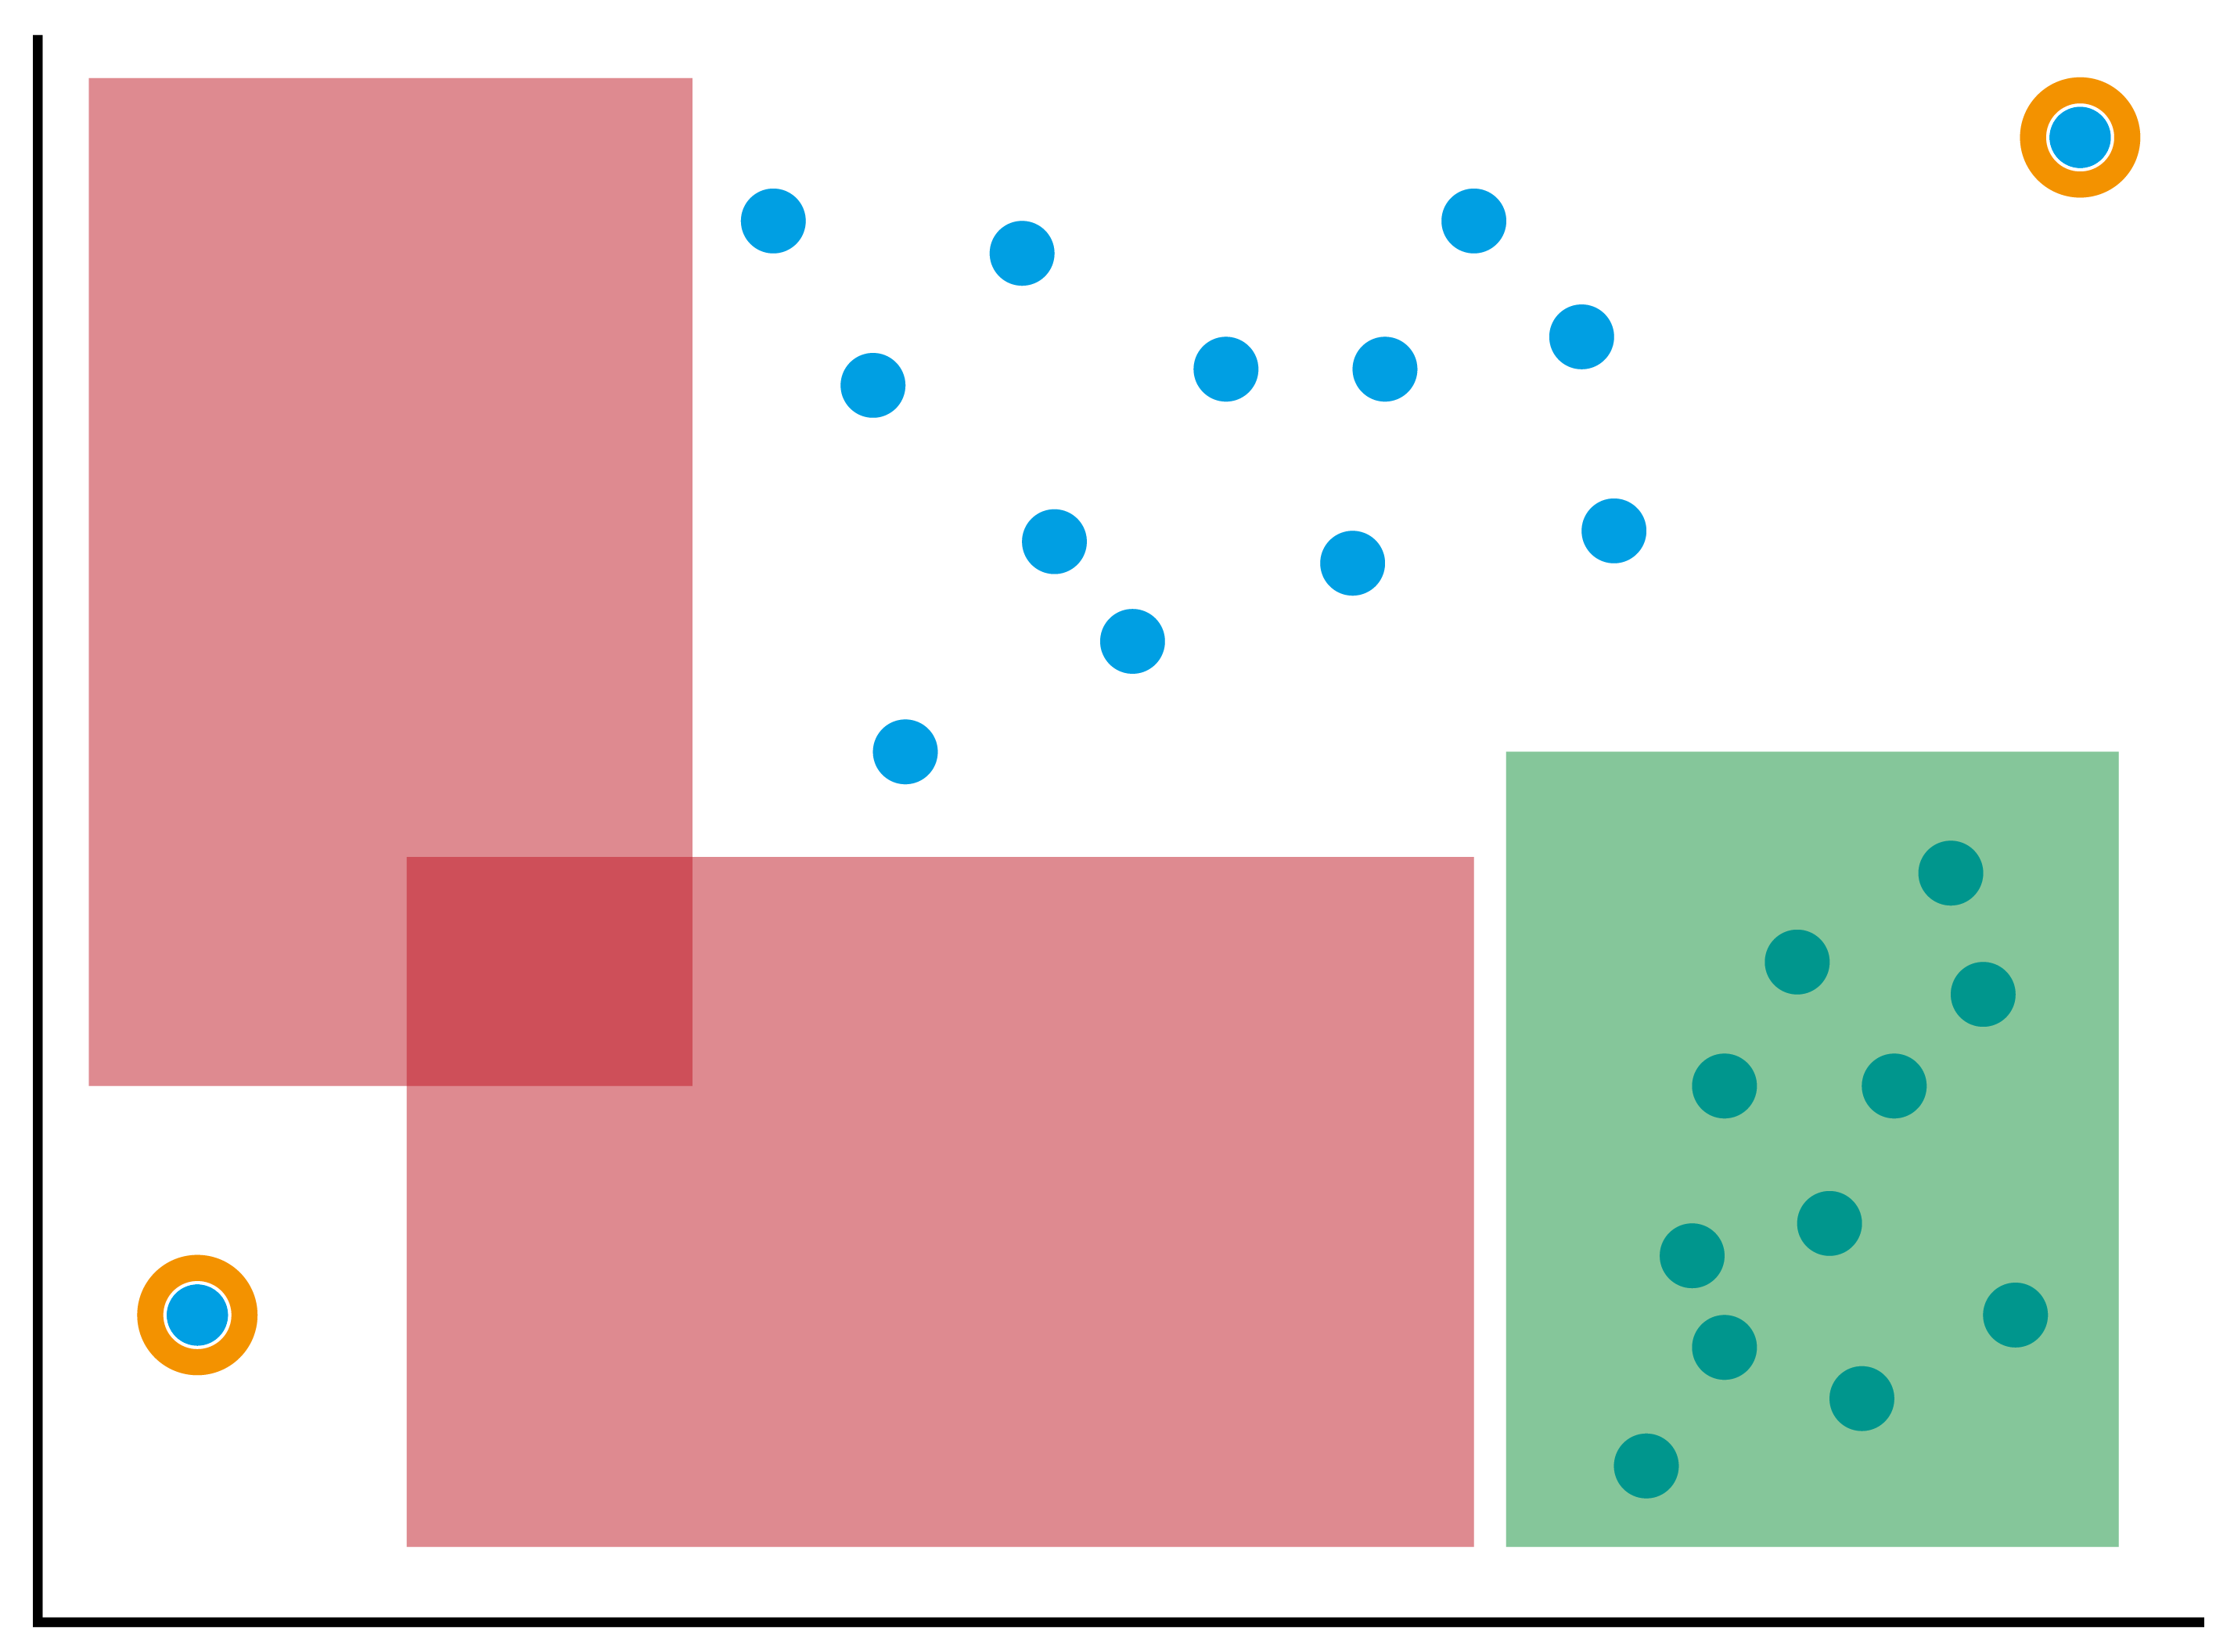
\includegraphics[width=0.5\textwidth]{images/konzeption-datenbereiche.png}
   \caption{Ein Scatterplot mit eingezeichneten Annotationsmöglichkeiten: Leere Bereiche (rot), nicht-leere Bereiche (grün) und einzelne Datenpunkte (orange).}
   \label{figure:datenbereiche}
\end{figure}

\subsection{API und Komponentenbeschreibung}
\label{section:konzeption:kommentare:api}

% konkreter. was gibt es für kommentare, wie unterscheiden sie sich, was ergeben sich für anforderungen daraus --> keine dynamischen daten, kein unvorhersehbares layout, keine aggregation, memento definieren, 

Um \emph{Wiederverwendbarkeit} über Komponenten hinweg zu fördern, sollten Kommentare sich möglichst auf die visualisierten Daten selbst beziehen (datenbezogene Kommentare) und nicht auf einen Bereich der Visualisierung (ortsbezogene Kommentare).

Komponenten, welche die Kommentarfunktion anbieten wollen, dürfen aus zwei Gründen keine externen Daten anzeigen (also beispielsweise die neuesten Tweets eines Twitter-Accounts): Erstens könnte der Kontext eines Kommentars sich ändern, etwa wenn Tweets gelöscht wurden. Die externen Daten unterliegen nicht der Kontrolle des Hilfesystems. Zweitens sind die externen Daten nicht im DaRe vorhanden, weswegen sie nicht über Komponenten hinweg wiederverwendet werden können. Dabei ist es unerheblich, ob die Komponente selbst externe Daten lädt oder externe Daten einer anderen Komponente anzeigt. Um den Fall von eigenen externen Daten für das Hilfesystem erkennbar zu machen, kann die Komponentenbeschreibung erweitert werden. Für den Fall von fremden externen Daten muss das Hilfesystem nach erfolgreicher Integration aller Visualisierungskomponenten selbst überprüfen, welche davon externe Daten laden und mit welchen diese über Links (Abschnitt~\ref{section:standderforschung:grundlagen:cruise_vizboard}) verbunden sind.

\subsubsection{Datenbezogene Bereichskommentare}

Damit Bereichskommentare Daten referenzieren können, müssen drei Voraussetzungen gegeben sein:

\begin{enumerate}
	\item Falls der Bereich leer ist, muss die grafische Repräsentation die Position als visuelles Mapping benutzen, damit eine Transformation zwischen kartesischen Koordinaten und Daten durchgeführt werden kann.
	\item In jedem Fall muss die Komponente eine Operation bereitstellen, welche kartesische Koordinaten $(x_1,y_1)$ in Datenbereiche (2000 \$, 14. Mai 1998) transformiert sowie deren Umkehrung. Komponenten sind \enquote{Black Boxes} und es kann deswegen keine Annahme über die verwendete Skala (linear oder logarithmisch) oder andere Interna getroffen werden. Aus diesem Grund ist es nicht möglich, aus Auswahlkoordinaten $(x_1,y_1,x_2,y_2)$ direkt auf Daten zu schließen.
	\item Die verwendeten Daten müssen im Data Repository gespeichert sein, da ansonsten keine Daten referenziert werden können. Aus diesem Grund darf weder die Komponente selbst Datenverarbeitung in Form von Aggregationen o.\,ä. durchführen, noch dürfen die Daten selbst bereits aggregiert in der Komponente ankommen.
\end{enumerate}

Erfüllt eine Komponente diese Bedingungen nicht vollständig, können nur ortsbezogene Bereichskommentare eingesetzt werden. Wenn datenbezogene Bereichskommentare angezeigt und von anderen Benutzern nachvollzogen werden sollen, muss das Hilfesystem die Komponente in den damals aktiven Zustand zurücksetzen können, da ansonsten die referenzierten Bereiche andere Daten enthalten können. Diese Tatsache führt zu weiteren Anforderungen an die Komponente:

\begin{enumerate}
	\setcounter{enumi}{3}
	\item Das Layout der Komponente muss vollständig reproduzierbar sein, also zum Beispiel kein Force Directed Layout \cite{Fruchterman1991}.
	\item Die Komponente muss der Laufzeitumgebung einen Weg zur Verfügung stellen, mit dem Zustände (wie z.\,B. Zentrum und Zoomlevel einer Karte) gespeichert und vollständig wiederhergestellt werden können.
\end{enumerate}

Bezüglich der letzten Anforderung bietet sich ein Memento-Pattern \cite{Gamma1994} an:

\begin{quote}
Without violating encapsulation, capture and externalize an object's internal state allowing the object to be restored to this state later.
\end{quote} 

Um Mementos umzusetzen, wird auf Properties zurückgegriffen. Eine Komponente muss ihren Zustand als Properties öffentlich machen und zwar so, dass durch Ändern von Properties kein inkonsistenter Zustand erreicht werden kann. Sie definiert das Format ihres Mementos, also welche Properties es ausmachen, in der Komponentenbeschreibung. Das Hilfesystem kann dann über die Methoden \texttt{getProperty(p)} und \texttt{setProperty(p,v)}, welche schon in der API der Komponente vorhanden sind, das Memento abrufen bzw. wiederherstellen. Eventuell registrierte PropertyLinks (Abschnitt~\ref{section:standderforschung:grundlagen:cruise_vizboard}) würden aktiviert und andere Komponenten ebenfalls verändert. Nachdem Events für eine Komponente zurückgehalten werden müssen, da sich das User Interface sonst ändern könnte, während der Benutzer Kommentare liest, haben PropertyLinks keinen Effekt.

\subsubsection{Ortsbezogene Bereichskommentare}

Datenbezogene Kommentare haben den Vorteil, dass sie auch in anderen Komponenten als der ursprünglich benutzten angezeigt werden können. Sie haben die Form eines Rechtecks, da so der Implementierungsaufwand für den Komponentenentwickler minimiert wird, obwohl prinzipiell beliebige geometrische Formen möglich sind. Andere Formen von Kommentaren sind zum Beispiel Pfeile oder Text, welche in der Nutzerstudie von \cite{Heer2007} am populärsten waren. Diese werden am besten als ortsbezogene Kommentare modelliert, da bei beiden Formen nicht eindeutig ist, welche Daten sie referenzieren. Siehe das Beispiel in Abbildung~\ref{figure:ortsbezogen}: Bezieht sich der Pfeil auf den Pixel am Ende der Pfeilspitze oder auf den roten Balken? Welche Daten soll der Text referenzieren?

\begin{figure}[htbp]
   \centering
   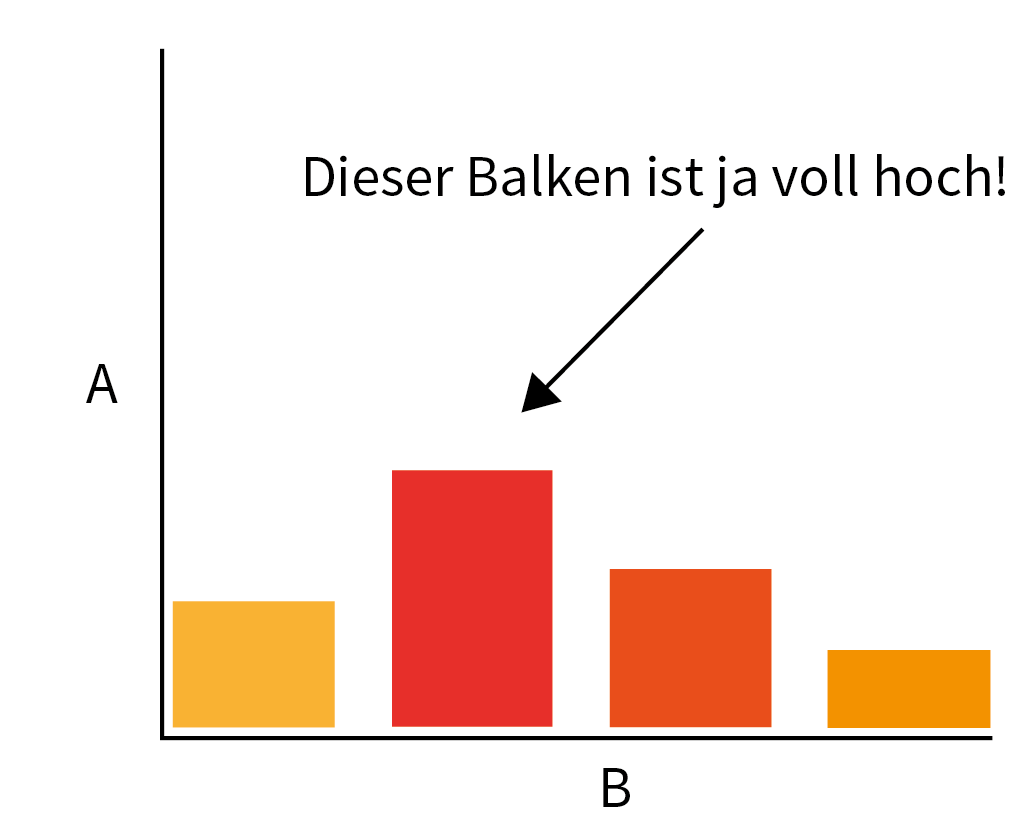
\includegraphics[width=0.5\textwidth]{images/konzeption-ortsbezogen.png}
   \caption{Ein ortsbezogener Kommentar mit Pfeil und Text}
   \label{figure:ortsbezogen}
\end{figure}

\subsubsection{Punktkommentare}

% speichern

Mit Datenpunkten verhält sich die Situation etwas einfacher als bei Bereichen. Es kann davon ausgegangen werden, dass Datenpunkte und deren DOM Elemente in einer $1:1$ (z.\,B. Balkendiagramm) oder $1:n$ (z.\,B. Scatterplot-Matrix) Relation stehen, da die Komponente sonst aggregieren würde. Im vorigen Abschnitt wurde für datenbezogene Kommentare ausgeschlossen, dass Komponenten Datenverarbeitung durchführen. Wenn der Komponentenentwickler im Markup der Komponente sichtbar machen würde, zu welchem Datenpunkt ein Element gehört, könnte das Hilfesystem mit Hilfe von CSS Selektoren diese finden und beispielsweise auswählbar machen, wenn ein Kommentar verfasst werden soll. Wird der Kommentar abgeschickt, muss die Komponente dem Hilfesystem zuerst mitteilen, welche Werte die visualisierten Attribute eines Datenpunkts haben. Das kann nicht automatisch aus dem DOM Element berechnet werden, weil der Maßstab unbekannt ist: Entspricht eine Fläche von $100\times100$~Pixel in der Treemap 10~Quadratmetern oder 1000~Hektar? Der Maßstab kann auch nicht in der Komponentenbeschreibung angegeben werden, weil von der Größe der Komponente abhängig ist. Bei einer Breite von 500~Pixel wäre er z.\,B. $1:100$, bei 250~Pixel Breite aber schon $1:200$. Die URI des Datenpunkts sowie die Werte der Attribute werden im Kommentar gespeichert, sodass sie in anderen Visualisierungen wiederverwendet werden können.

% markup

Zuvor muss allerdings noch geklärt werden, auf welche Weise der Komponentenentwickler die URIs im Markup sichtbar machen soll. Prinzipiell kommen dafür alle Möglichkeiten in Frage, die mit Hilfe von CSS ausgelesen werden können. Dazu gehören HTML Markup Elemente wie \texttt{id} oder Datenattribute \texttt{data-*}, aber auch Microformats\footnote{\url{http://microformats.org/}} oder RDFa \cite{W3C2012}. Microformats werden ausgeschlossen, da bei diesen das Vokabular vorgegeben ist, während bei RDFa nur die Syntax definiert wird. Eine URI ist kein gültiger Wert für die \texttt{id} eines DOM Elements, deswegen wird auch sie ausgeschlossen. RDFa hat gegenüber Datatype Propertiesn den Vorteil, dass so auch zusätzliche Informationen über den Datenpunkt (beispielsweise das Label) ins Markup integriert werden können. Auf diese Weise kann das Hilfesystem unter Umständen den einen oder anderen Aufruf des DaRes einsparen und stattdessen HTML parsen, was zur Geschwindigkeit der Anwendung beiträgt.

% laden
Beim Laden von Punktkommentaren zählt das Hilfesystem erst die Anzahl von Kommentaren pro Datenpunkt und stellt diese Anzahl über dem visualisierten Datenpunkt dar. Das ist möglich, weil über die URI in Kombination mit CSS Selektoren die entsprechenden DOM Elemente identifiziert werden können.


\subsection{User Interface und Interaktion}
\label{section:konzeption:kommentare:ui}

% ### user interface & interaktion

In der Titelleiste gibt es zwei Buttons mit einem Sprechblasen-Icon, einmal ist eine Zahl darin (Kommentare ansehen) und einmal ein Pluszeichen (Kommentar hinzufügen). Eine ständig sichtbare textuelle Beschreibung wäre offensichtlicher, kann aber aufgrund des geringen Platzangebots nur mit einem Tooltip umgesetzt werden.

Wenn der Benutzer einen Kommentar verfassen will, erscheint eine Sidebar mit einer Textbox, Controls um die Annotationsform zu ändern (Auswahl, Rechteck, Pfeil, Text) und einem Button zum Bestätigen (Abbildung~\ref{figure:kommentare-step4}). Der Benutzer kann nun ein oder mehrere Rechtecke in der Visualisierung oder Datenpunkte markieren (linker Balken in Abbildung~\ref{figure:kommentare-step4}). Das Hilfesystem setzt die Komponente in den Ausgangszustand zurück, sobald der Benutzer bestätigt oder abgebrochen hat.

\begin{figure}[htbp]
   \centering
   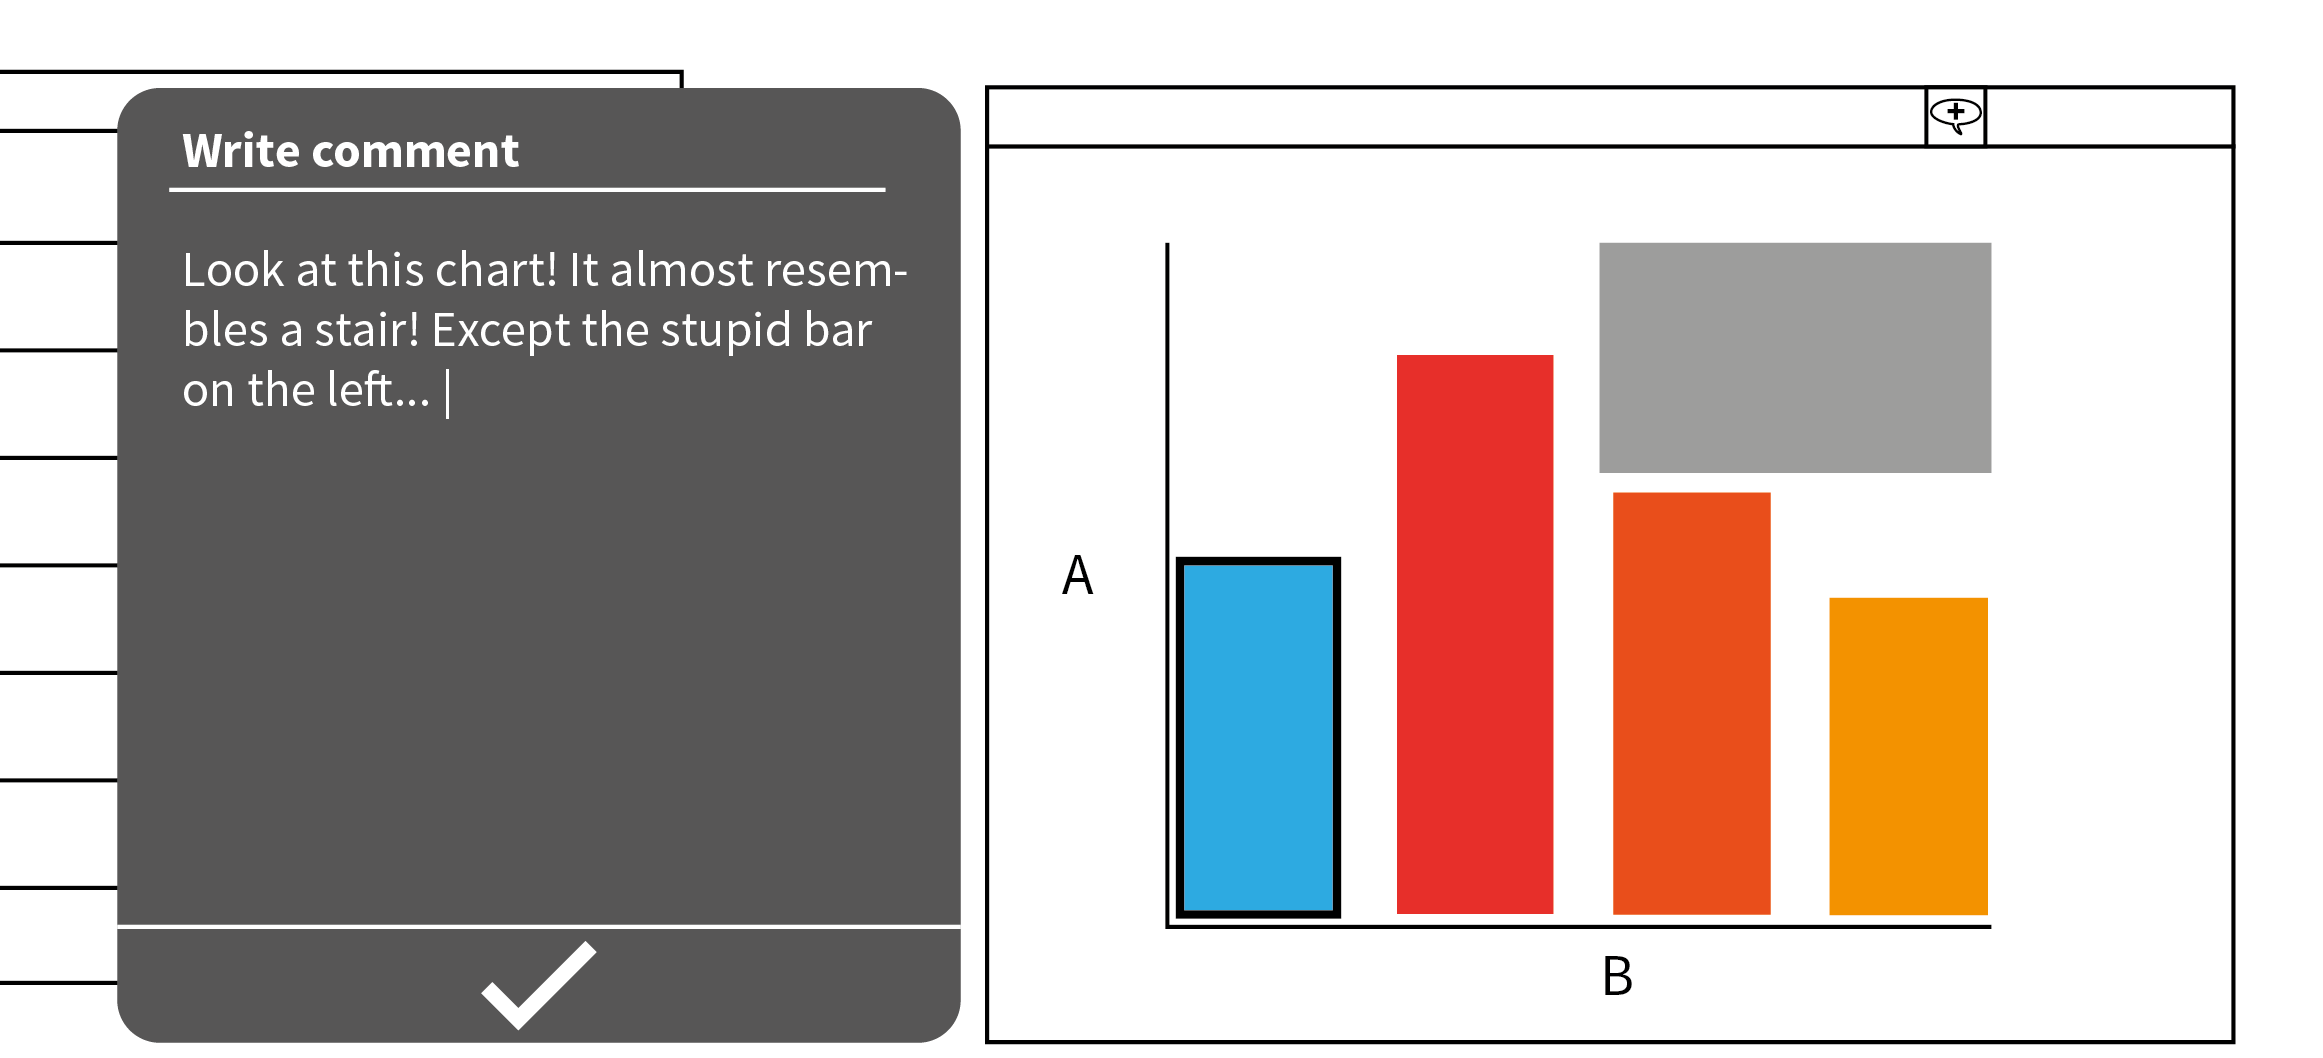
\includegraphics[width=0.75\textwidth]{images/konzeption-kommentare-step4.png}
   \caption{UI Mockup: Kommentar hinzufügen}
   \label{figure:kommentare-step4}
\end{figure}

Möchte der Benutzer Kommentare anderer lesen, wechselt der Inhalt der Sidebar zu einer Liste aller in dieser Komponente bzw. zu diesen Daten verfassten Kommentare (Abbildung~\ref{figure:kommentare-step2}). Ein Kommentar zeigt folgende Elemente.

\begin{itemize}
	\item Linke Spalte
	\begin{itemize}
		\item ID des Kommentars: Diese ist zur Referenzierung notwendig.
		\item Avatar des Benutzers und Benutzername: Diese sollen das Vertrauen der Benutzer untereinander erhöhen und so die Qualität der Kommentare verbessern \cite{Chiu2006}. Gespeichert und abgerufen werden sie in der Benutzerverwaltung von VizBoard.
		\item Datum der Erstellung oder letzten Editierung, was jünger ist. Wurde editiert, ist das Datum kursiv geschrieben.
		\item Editieren/Löschen-Buttons, falls der Kommentar selbst verfasst wurde.
		\item Antworten: Eine zweite Möglichkeit als die ID des Kommentars einzutippen. Die UI wechselt zu \enquote{Kommentar verfassen} und inkludiert die ID des betreffenden Kommentars.
		\item Annotationen anzeigen: Zeigt die Annotationen des Kommentars in der Visualisierung.
		\item Voting: Ein Benutzer kann einen fremden Kommentar genau einmal bewerten. Die Anzahl der Stimmen wird ebenfalls angezeigt. Anstatt \enquote{upvote/downvote} wird hier die Wortkombination \enquote{agree/disagree} verwendet, da bei der Nutzerstudie ersteres selten mit \enquote{bewerten} und manchmal mit \enquote{scrollen} assoziiert wurde.
	\end{itemize}
	\item Rechte Spalte
	\begin{itemize}
		\item Kommentartext mit Referenzen (durch \texttt{\#hash} gekennzeichnet) und URLs (unterstrichen).
	\end{itemize}
\end{itemize}

Referenzen auf andere Kommentare können angeklickt werden. Dann wird der gewählte Kommentar in der Sidebar angezeigt und die Titelleiste enthält einen Zurück-Button, mit dem der vorherige Zustand wiederhergestellt werden kann.

Die Datenpunkte in der Visualisierung werden mit einer Anzeige, wie viele Kommentare dazu vorhanden sind, erweitert (Abbildung~\ref{figure:kommentare-step2}). Sie sind oben rechts platziert, um so an iOS Badges zu erinnern und damit Assoziationen zu einem Hinweis zu wecken.

\begin{figure}[htbp]
   \centering
   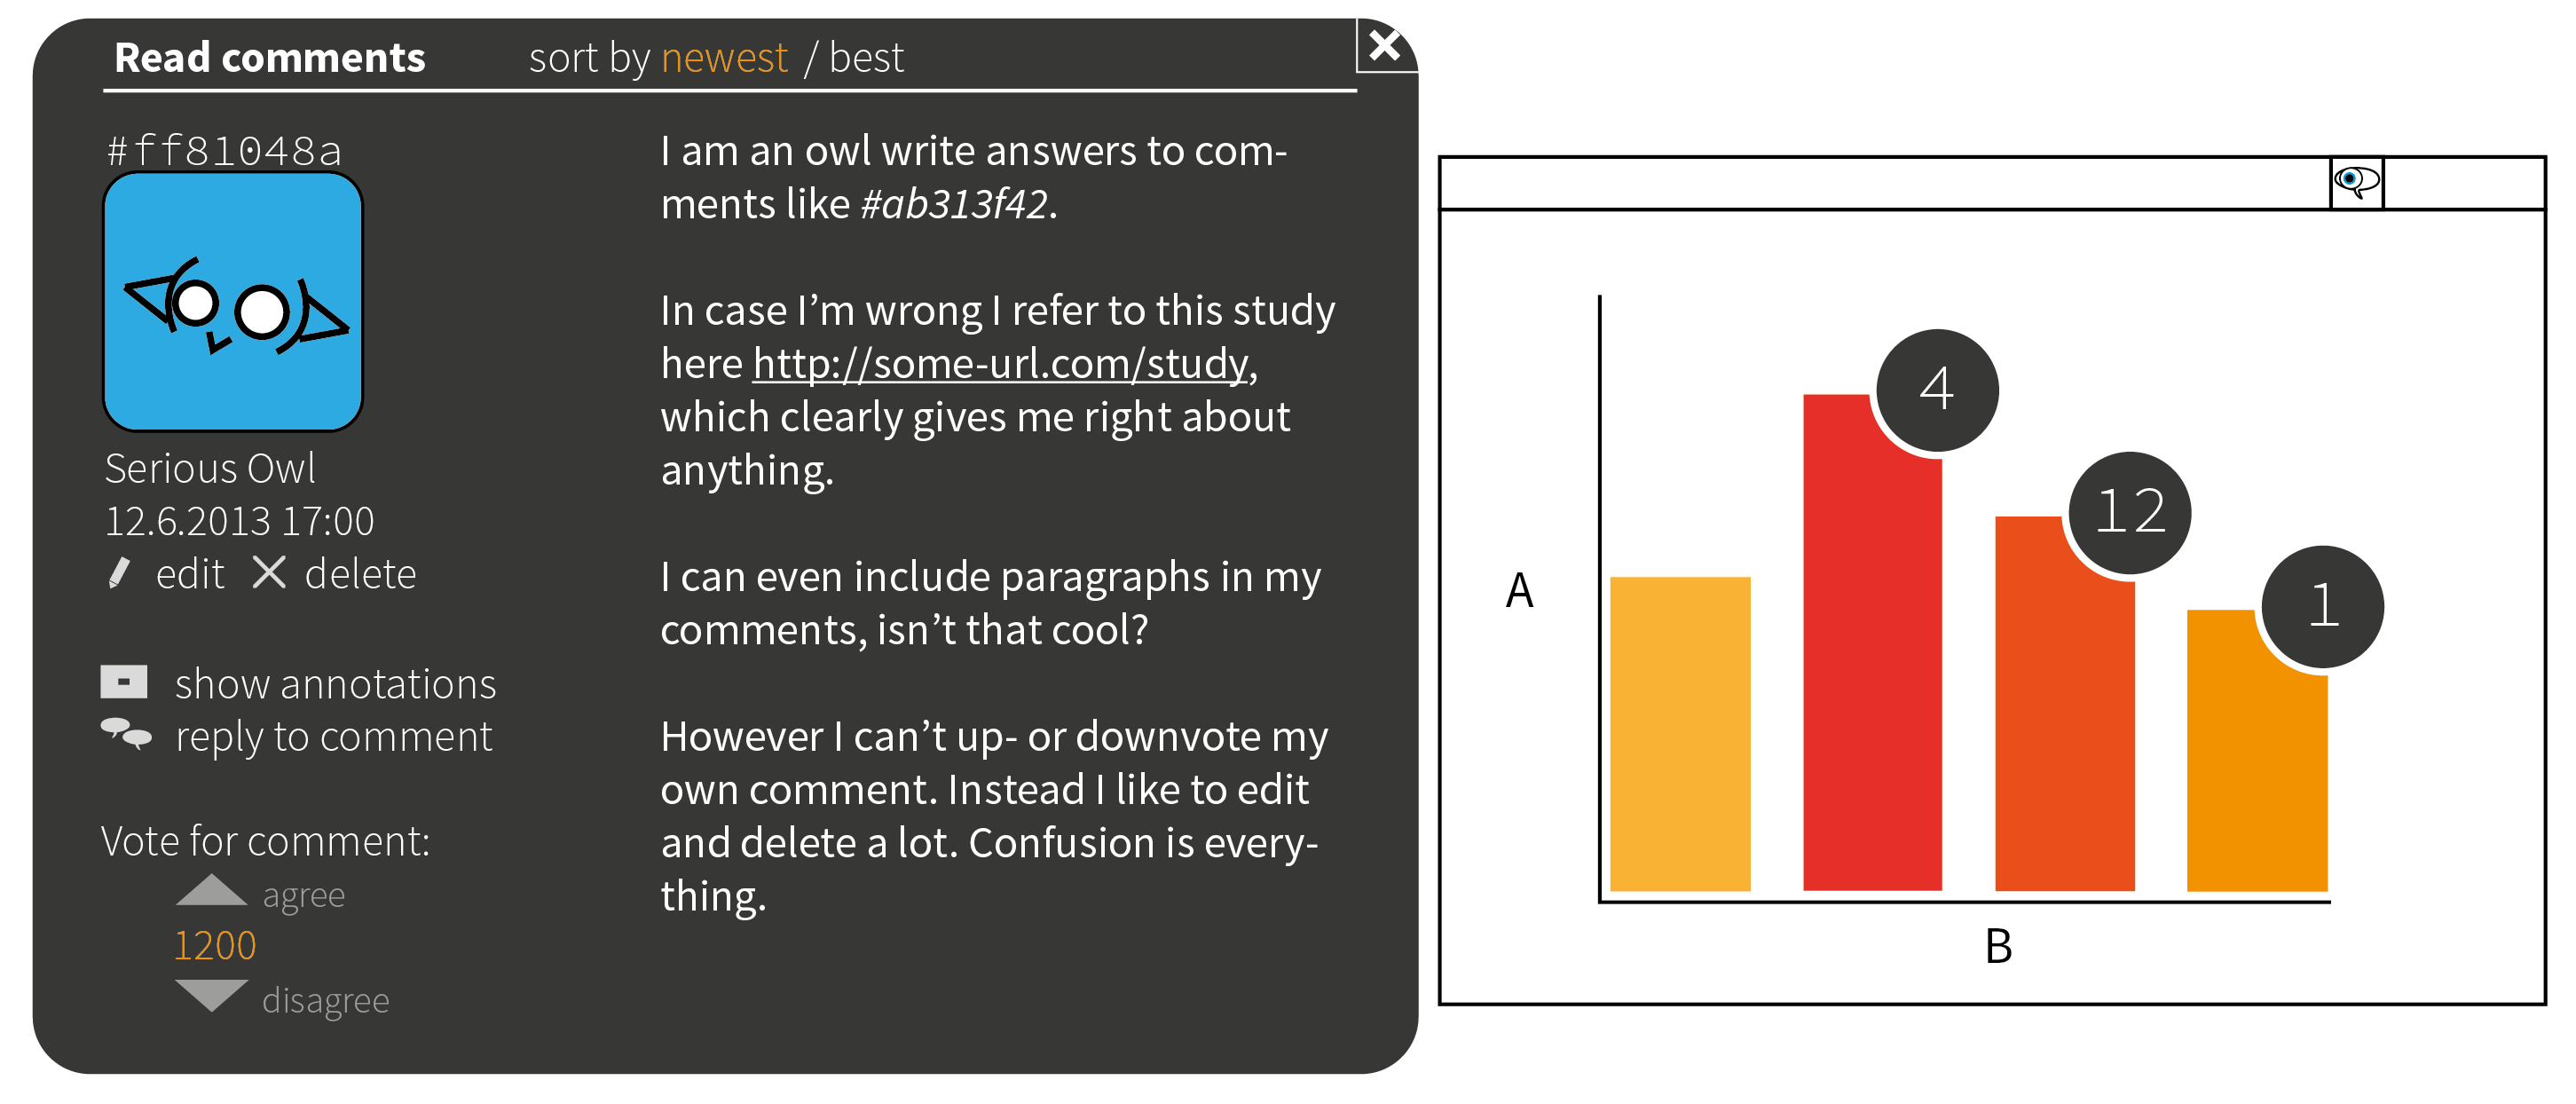
\includegraphics[width=0.75\textwidth]{images/konzeption-kommentare-step2.png}
   \caption{UI Mockup: Anzeige aller Kommentare}
   \label{figure:kommentare-step2}
\end{figure}

Diese Badges können angeklickt werden. Die Sidebar enthält dann alle Kommentare, die sich auf den gewählten Datenpunkt beziehen (Abbildung~\ref{figure:kommentare-step3c}).

\begin{figure}[htbp]
   \centering
   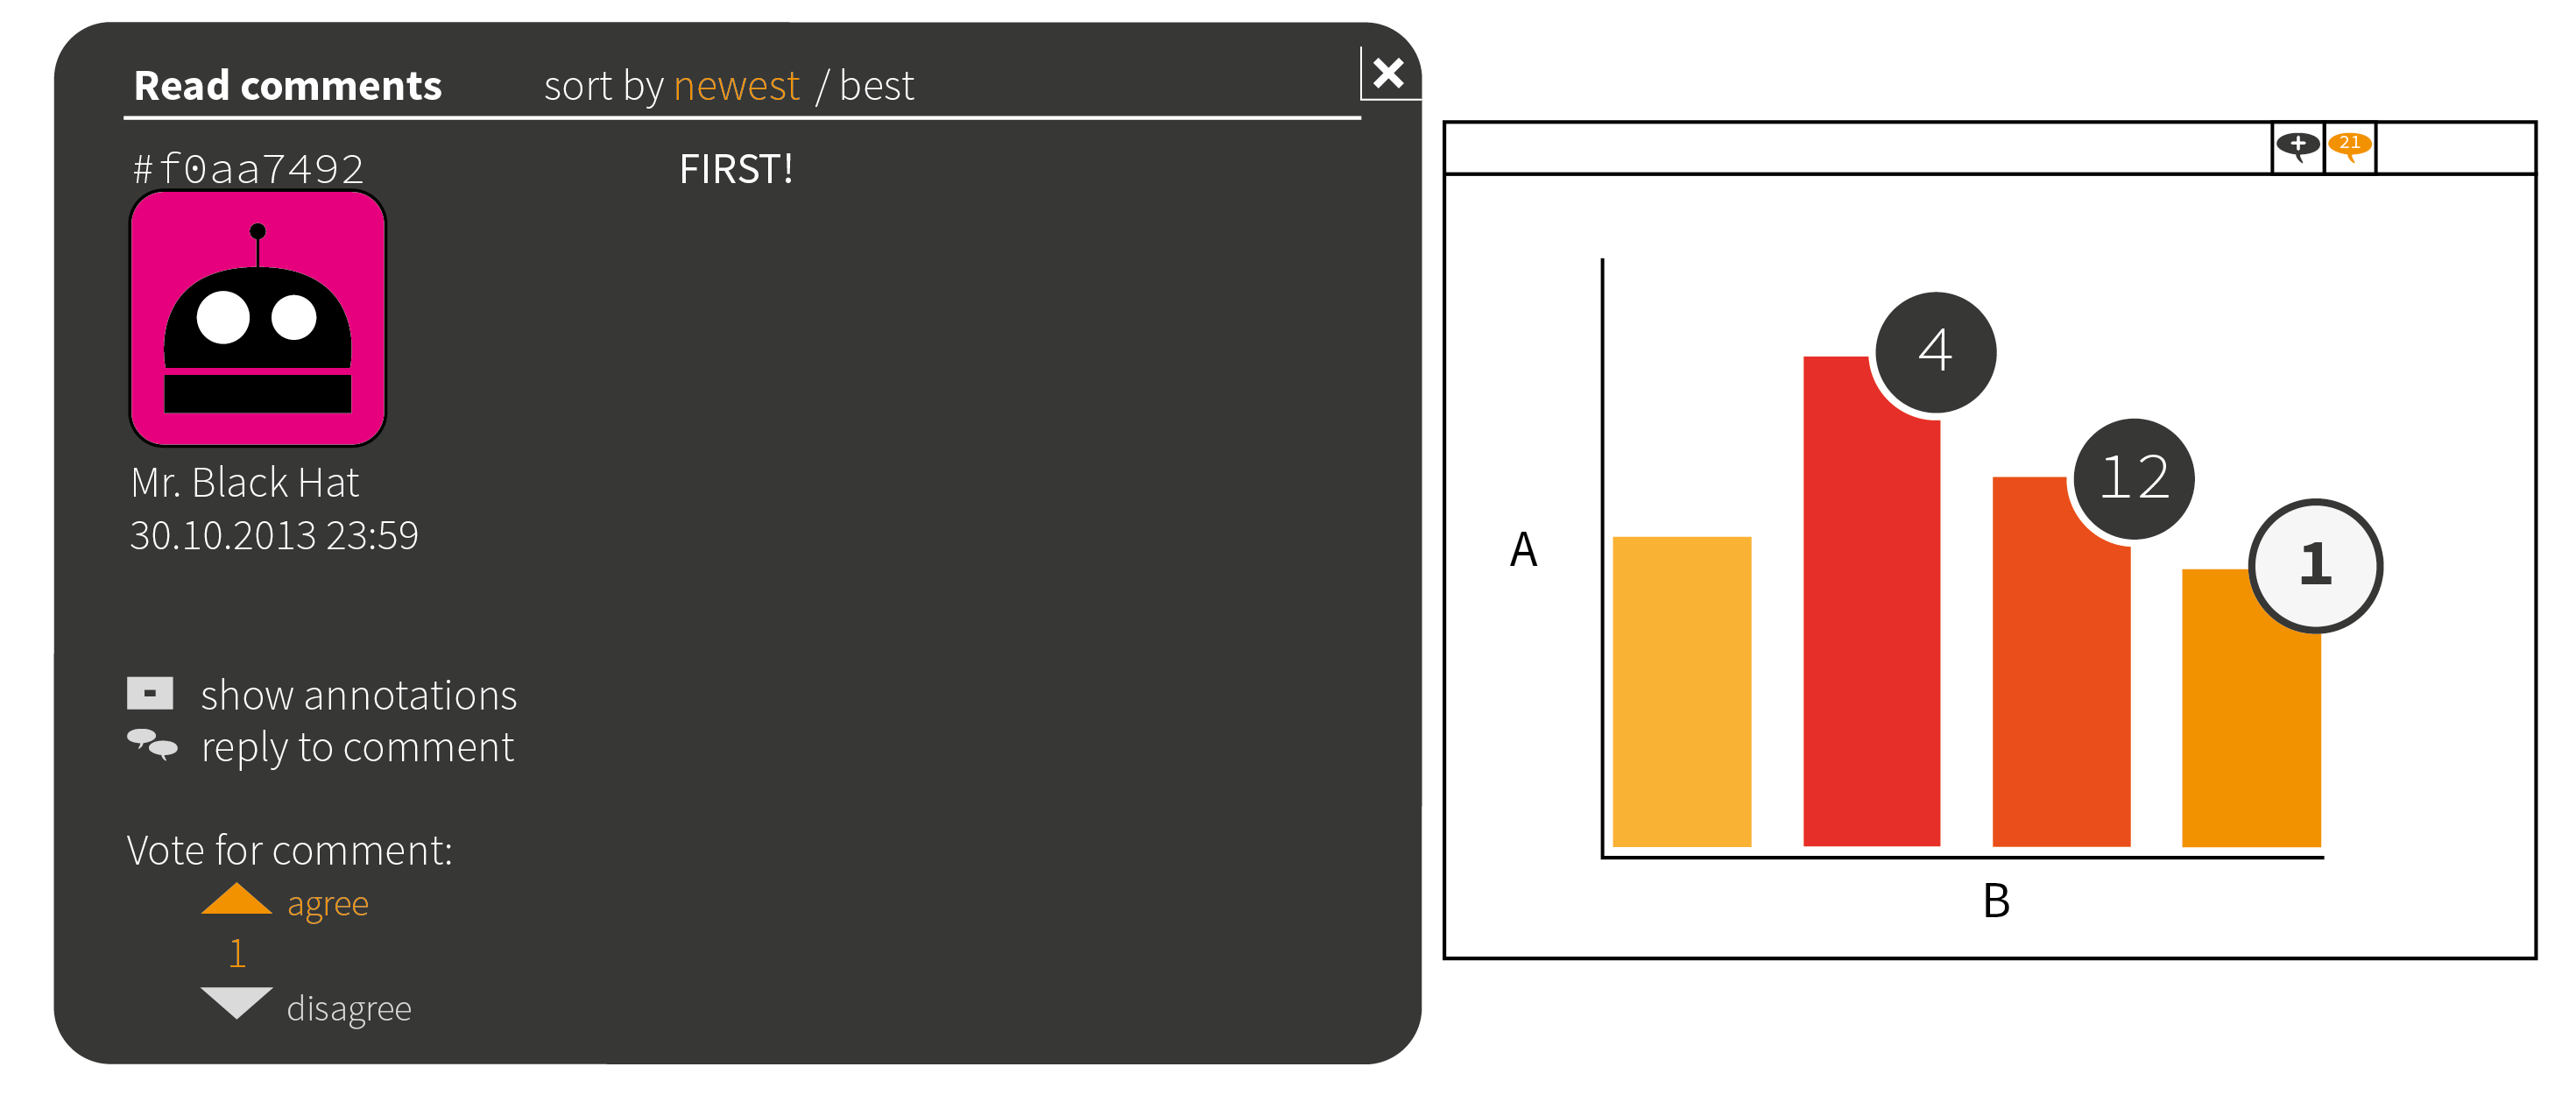
\includegraphics[width=0.75\textwidth]{images/konzeption-kommentare-step3c.png}
   \caption{UI Mockup: Alle Kommentare zum ausgewählten Datenpunkt}
   \label{figure:kommentare-step3c}
\end{figure}

Annotationen eines Kommentars müssen durch einen Klick auf den Button \enquote{show annotations} angezeigt werden. Der Viewport der Visualisierung wird dann abgedunkelt und nur die Annotationen des ausgewählten Kommentars bleiben sichtbar (Abbildung~\ref{figure:kommentare-step3a}).

\begin{figure}[htbp]
   \centering
   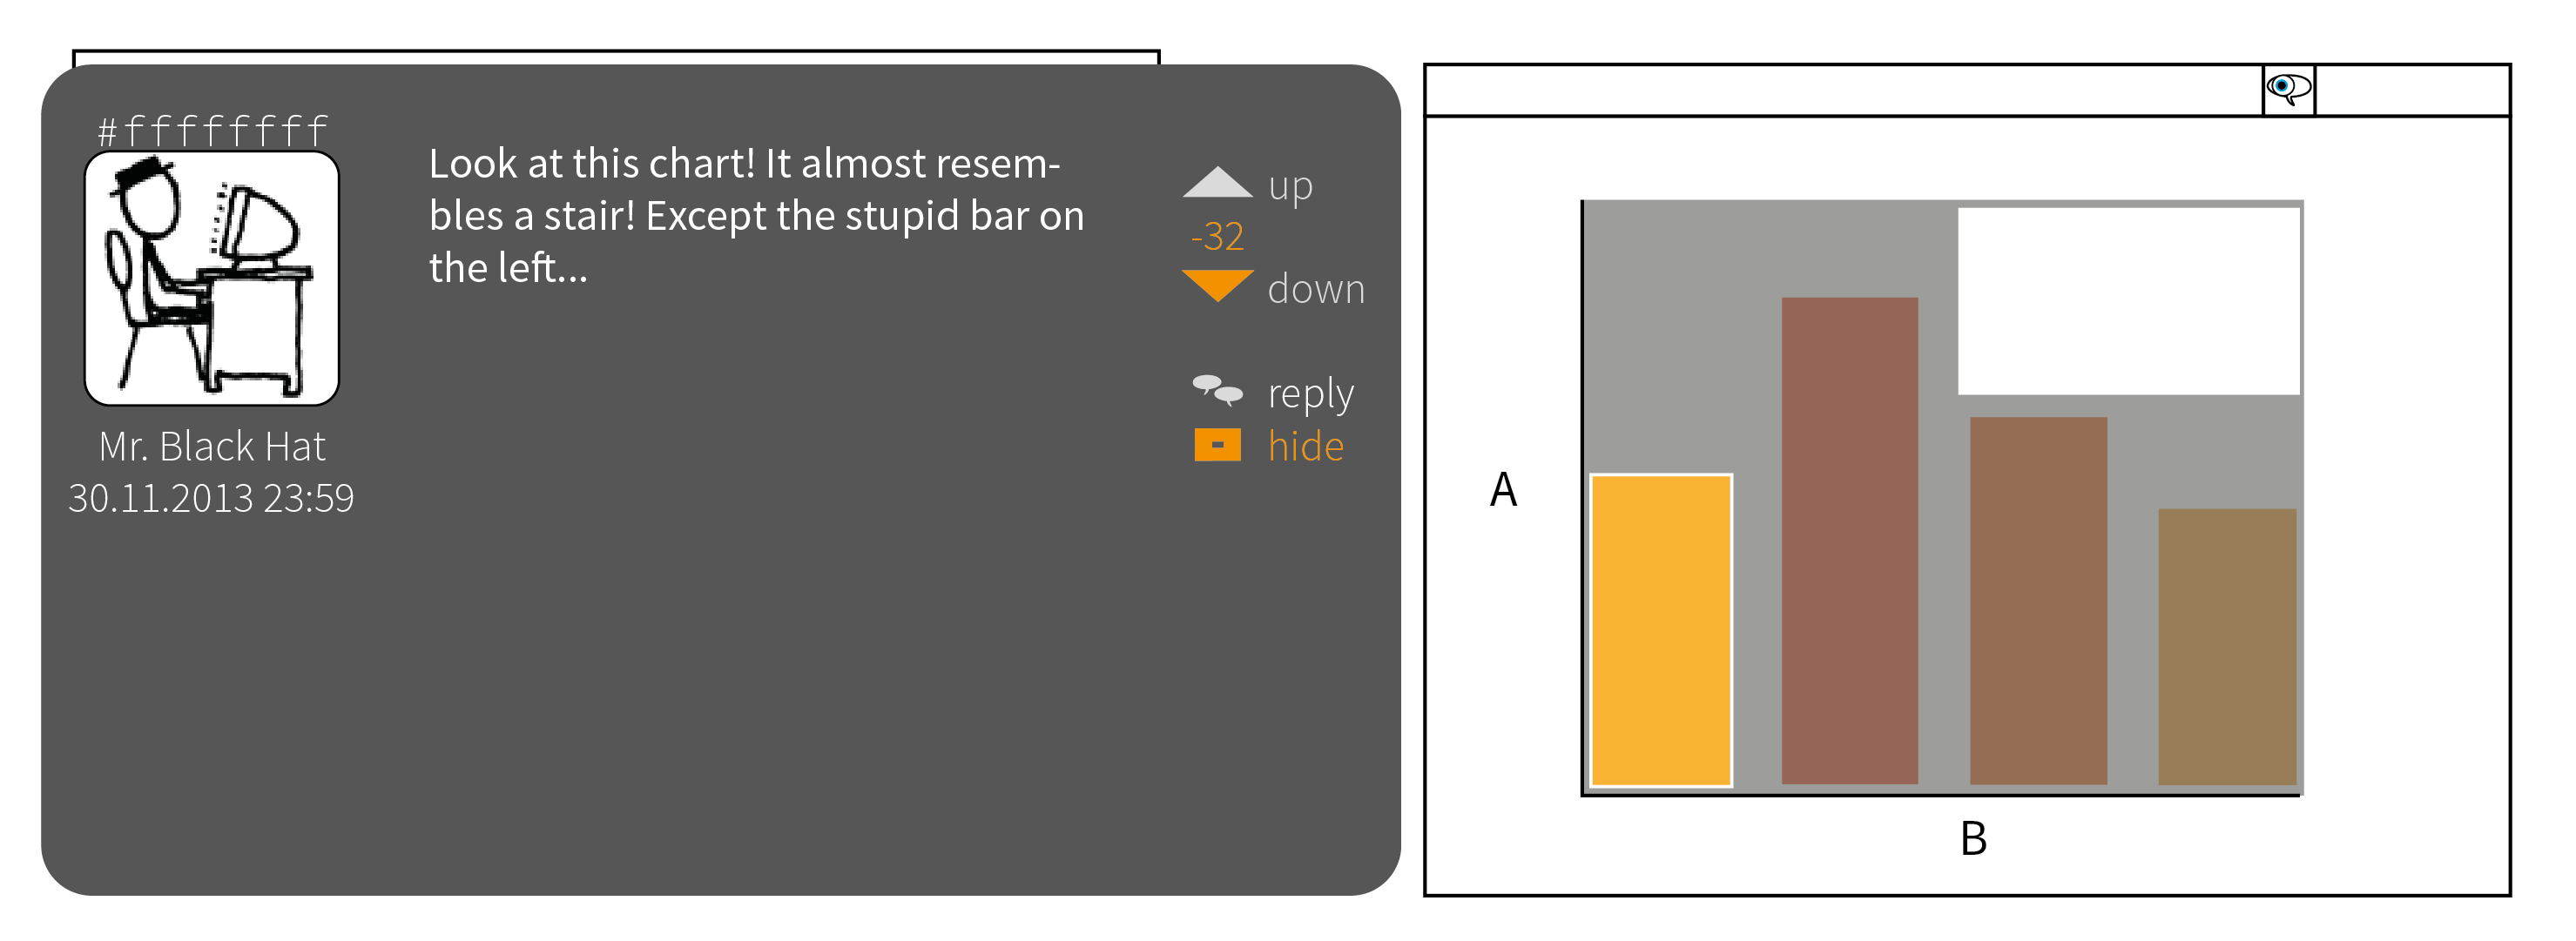
\includegraphics[width=0.75\textwidth]{images/konzeption-kommentare-step3a.png}
   \caption{UI Mockup: Ausgewählter Kommentar mit referenziertem Bereich und Datenpunkten}
   \label{figure:kommentare-step3a}
\end{figure}

\subsection{Backend}
\label{section:konzeption:kommentare:backend}

% ### backend

% welche daten enthält ein gespeichertes kommentar?

Den Ausführungen in den Abschnitten~\ref{section:konzeption:kommentare:features} und~\ref{section:konzeption:kommentare:api} nach enthält ein abgespeichertes Kommentar im DaRe folgende Daten:

\begin{itemize}
	\item ID des Kommentars, um darauf verweisen zu können.
	\item ID der Komponente, in der der Kommentar verfasst wurde. Das ist notwendig um ortsbezogene Kommentare wiederherstellen zu können. Bei datenbezogenen Kommentaren kann eventuell ein Verweis auf die ursprüngliche Komponente erstellt werden.
	\item ID des Datensatzes, der visualisiert wurde
	\item ID des Verfassers
	\item URIs der Datatype Properties, die visualisiert wurden
	\item Memento der Komponente zum Zeitpunkt des Kommentars
	\item \textit{Für jede Version des Kommentars}
	\begin{itemize}
		\item Versionsnummer
		\item Zeitpunkt
		\item Kommentartext
		\item \textit{Wenn ortsbezogene Elemente vorhanden}
		\begin{itemize}
			\item Größe der Visualisierung zum Zeitpunkt des Kommentars, um die Auswahlrechtecke entsprechend skalieren zu können
			\item Für jedes Element
			\begin{itemize}
				\item Wenn Pfeil: ($x_1,y_1,x_2,y_2$)
				\item Wenn Text: Text, $(x,y)$
				\item Wenn Rechteck: ($x_1,y_1,x_2,y_2$)
			\end{itemize}
		\end{itemize}
	\item \textit{Für jedes datenbezogene Element}
		\begin{itemize}
			\item Grenzwerte der visualisierten Datatype Properties. Ist ein Datatype Property nominalen Typs, besitzt also keine inhärente Ordnung (z.\,B. Länder), muss eine Menge von Datenpunkten angegeben werden.
		\end{itemize}
	\item \textit{Für jeden Datenpunkt}
		\begin{itemize}
			\item URI
			\item Werte der visualisierten Datatype Properties
		\end{itemize}
	\end{itemize}
\end{itemize}

% wie läuft das mit speichern?

Hat ein Benutzer Bereiche und Datenpunkte referenziert, sowie einen Kommentar geschrieben, sammelt das Hilfesystem die eben beschriebenen Daten der Komponente und sendet sie ans Data Repository. Das Speichern und Laden von Kommentaren liegt in dessen Verantwortung. 

% wie läuft das mit laden, vor allem wenn kommentare in anderer komponente gemacht wurden?

Sollen Kommentare angezeigt werden, schickt das Hilfesystem eine entsprechende Anfrage ans DaRe und empfängt die Daten aller relevanten Kommentare. Für ortsbezogene Bereichskommentare ist nichts weiter zu tun, sie können direkt in dieser Komponente gerendert werden. Um datenbezogene Bereichskommentare anzuzeigen, muss das Hilfesystem zuerst die Datengrenzen in Koordinaten in der Visualisierung transformieren lassen. Bei Punktkommentaren ist dies nicht nötig, weil das Hilfesystem über CSS Selektoren herausfinden kann, wo sie sich befinden sollen.

% event broker suspend/resume

Um zu gewährleisten, dass der Benutzer störungsfrei Kommentare lesen kann, muss das Hilfesystem den Event Broker (Abschnitt~\ref{section:standderforschung:grundlagen:cruise_vizboard}) veranlassen können, anfallende Events nicht weiterzuleiten (\enquote{suspend}) und in einer FIFO Warteschlange zwischenzulagern. Ansonsten könnte der Fall eintreten, dass die Komponente aktualisiert wird, während der Benutzer Kommentare zu den Daten liest oder eine andere Hilfe in Anspruch nimmt. Diese Funktion ist in Grundzügen bereits für das Handling von PropertyLinks vorhanden \cite[S. 161]{Pietschmann2012}. Nachdem die Kommentar UI geschlossen wurde, kann der Event Broker die gespeicherten Events weiterleiten (\enquote{resume}). Sie werden einfach in Reihenfolge weitergegeben. Das hat den Nachteil, dass sich das User Interface mehrmals schnell ändern könnte, bis alle pausierten Events abgearbeitet sind. Eine andere Möglichkeit wäre die Pausierungsfunktion auf Komponentenebene umzusetzen. Das würde allerdings Mehraufwand sowohl für den Komponentenentwickler, der die entsprechenden Methoden implementieren müste, als auch für das Hilfesystem, welches jede Komponente einzeln ansprechen muss, bedeuten.

\subsubsection{Weitere Nutzung}

% wie können kommentare noch genutzt werden?

Kommentare können auch Metainformationen über die Daten oder Komponente enthalten \cite{Chen2009}. Es wäre denkbar, mittels automatischer Textklassifikation \cite{Sebastiani2002} diese Kommentare zu identifizieren und als positiv oder negativ zu kategorisieren. Daraus ließe sich wiederum eine Bewertung für die Kombination (Datensatz, Komponente) berechnen\footnote{Am einfachsten ginge das indem bei Null gestartet wird und für jeden positiven Kommentar der Zähler um eins erhöht und jeden Negativen um eins verringert wird.}. Der errechnete Wert könnte in Zukunft beim Ranking einer Komponente für einen ausgewählten Datensatz berücksichtigt werden. Wenn der Aufwand dafür gerechtfertigt werden kann, ist es auch möglich, eine -- zuvor definierte -- Ontologie aus Kommentaren zu extrahieren \cite{Alani2003}. Diese könnte zum Beispiel das Qualitätsmanagement von Komponenten automatisieren. Denkbar wäre, dass aus Kommentaren automatisch extrahiert wird, worüber sich die Benutzer beschweren. Ab einem Schwellwert kann dann der Komponentenentwickler informiert werden.

\section{History}
\label{section:konzeption:history}

% warum undo/redo?

In den verwandten Arbeiten (Abschnitt~\ref{section:standderforschung:verwandte_arbeiten}) wurde mehrmals empfohlen, dem Benutzer Undo/Redo von getätigten Aktionen zu ermöglichen. So können unerwünschte Ergebnisse einfach rückgängig gemacht werden. In diesem Abschnitt wird untersucht, wie in einem CRUISe Mashup, in dem die Komponenten lose gekoppelt sind, ein kompositionsübergreifendes Undo/Redo umgesetzt werden kann. Die Granularitätsstufe entspricht dabei Nutzerinteraktionen beziehungsweise zusammenhängenden anstatt einzelnen Events oder Operationen. Das sollte sich wie in den verwandten Arbeiten von Grammel \cite{Grammel2012} vorgeschlagen mit dem mentalen Modell des Benutzers decken, da für ihn Events und Operationen unsichtbar sind. Als Beispiel wird die Komposition in Abbildung~\ref{figure:dependency-graph-example} verwendet.

\begin{figure}[htbp]
   \centering
   \includegraphics[width=0.75\textwidth]{images/konzeption-dependency-graph-example.png}
   \caption{Beispielhafte Komposition}
   \label{figure:dependency-graph-example}
\end{figure}

In Abschnitt~\ref{section:konzeption:kommentare:api} wurde ein Memento-Pattern für Komponenten eingeführt. Damit kann das Hilfesystem Zustände von Komponenten abrufen, speichern und wiederherstellen. Im Folgenden wird davon ausgegangen, dass diese Mementos ausreichen, um eine Komponente von einem konsistenten Zustand in einen anderen konsistenten Zustand zu überführen (und beispielsweise keine Operationen ausgeführt werden müssen). Es stellt sich allerdings die Frage, wann die Mementos der Komponenten abgerufen werden sollen. Prinzipiell kann es vor oder nach einem Event (welches Operationen aufruft, die potentiell den Zustand der Komponente ändern) passieren.

% vorher - klappt nicht, funkt der dev dazwischen 

\textbf{Vor} einem Event die Mementos abzurufen ist nicht möglich, da ein Event erst registriert wird, wenn die Nachricht im Event Broker ankommt. Zu diesem Zeitpunkt kann eine Komponente ihren Zustand bereits geändert haben. Das Hilfesystem könnte eigene Event Handler auf die Operationen der aktionsrelevanten UI Elemente registrieren und so bemerken, wann ein Event ausgelöst wird. Allerdings kann das Hilfesystem erst Event Handler registrieren, wenn die Komponente initialisiert wurde. Zu diesem Zeitpunkt wurde der DOM geladen und Event Handler des Komponentenentwicklers registriert. Die Event Handler des Hilfesystems würden zwangsläufig nach den Handlern des Entwicklers ausgeführt. Wenn es soweit ist, könnte die Komponente schon ihren Zustand verändert haben und das Memento enthält nicht die gewünschten Attributwerte.

Eine mögliche Lösung wäre den Lebenszyklus der Komponenten zu modifizieren. Es könnte ein Zustand \emph{Rendered} zwischen \emph{Integrated} und \emph{Active} eingefügt werden (Abbildung~\ref{figure:cruise-lifecycle}), bei dem der DOM der Komponente vollständig vorhanden sein, aber Event Handler noch nicht registriert sein sollen. Zu diesem Zeitpunkt könnte das Hilfesystem seine Handler vor jenen des Komponentenentwicklers registrieren, die dann auch als erstes ausgeführt würden. Problematisch ist allerdings, wenn eine Komponente zur Laufzeit DOM Elemente erstellt und Event Handler registriert. Dieses Verhalten müsste man verbieten, um sicherzustellen dass Handler des Hilfesystems immer zuerst ausgeführt werden. Das ist aber nicht wünschenswert, weil diese Vorgabe möglicherweise große Anpassungen des Komponentencodes nötig macht und oft auch gar nicht umsetzbar ist.

\begin{figure}[htbp]
   \centering
   \includegraphics[width=0.75\textwidth]{images/konzeption-cruise-lifecycle.png}
   \caption{UI Mockup: Modifizierter CRUISe Komponentenlebenszyklus}
   \label{figure:cruise-lifecycle}
\end{figure}

% nachher

Es bleibt die Möglichkeit \textbf{nach} einem Event Mementos abzurufen. Zunächst ist es schwierig festzustellen, wann \enquote{nach} einem Event überhaupt ist. Events können in dem Sinne kaskadieren, als dass sie Operationen aufrufen, die weitere Events feuern, die wiederum Operationen ausführen, die selbst Events feuern und so weiter. Aus dem Kommunikationsmodell kann a priori nicht eindeutig bestimmt werden, welche Events nach einem Event $e_0$ zu erwarten sind. Das ist eine Folge des \enquote{Black Box} Prinzips der Komponenten. Im folgenden Abschnitt wird ein Konzept erarbeitet, mit dem das Hilfesystem kaskadierende Events identifizieren kann.

\subsection{Backend}

% voraussetzungen

Ein Ansatz zur Lösung des Problems ist anfangs einen Abhängigkeitsgraphen aus dem Kommunikationsmodell zu generieren (Abbildung~\ref{figure:dependency-graph}). Dazu werden alle Events und Operationen der Komponenten gesammelt. Es führen Kanten von Events zu Operationen, wenn ein Link im Kommunikationsmodell besteht. Wenn ein Event von einer Operation abhängig ist (z.\,B. $e_1$ von $o_1$), wird ein Link von der Operation zum Event eingefügt. Dem Hilfesystem ist das bekannt, weil in der Komponentenbeschreibung Events abhängig von Aktionen beschrieben zu den Aktionen Operationen So kann das Hilfesystem bestimmen, welche Events später noch gefeuert werden könnten. Außerdem werden Nachrichten, die zwischen Komponenten ausgetauscht werden, so erweitert, dass sie zusätzlich die aufrufende Operation und einen Timestamp enthalten.

\begin{figure}[htbp]
   \centering
   \includegraphics[width=0.5\textwidth]{images/konzeption-dependency-graph.png}
   \caption{Abhängigkeitsgraph der beispielhaften Komposition mit möglichem Ablauf der Events und Operationen}
   \label{figure:dependency-graph}
\end{figure}


% algorithmus

Abbildung~\ref{figure:dependency-graph} zeigt einen beispielhaften Ablauf. $e_3$ und $e_4$ werden gefeuert, weil eine Aktion in Komponente A ausgeführt wurde. Der Algorithmus funktioniert wie folgt:

\begin{enumerate}
	\item Komponente A feuert Event $e_1$.
	\item Das Hilfesystem registriert die Nachricht $e_1$ und bestimmt zunächst aus dem Abhängigkeitsgraphen, ob A eine unabhängige Komponente ist und ob noch weitere (auf $e_1$ zurückführende) Nachrichten zu erwarten sind. Da dies der Fall ist, fügt das Hilfesystem $e_1$ in eine neu erstellte Collection hinzu und legt ein Timeout von $t$ Millisekunden fest. Läuft es ab, fährt der Algorithmus bei Schritt 7 fort. Außerdem wird $e_1$ bis dorthin der Operation $o_4$ von C zugeordnet.
	\item Innerhalb des Timeouts $t$ feuert Komponente C Event $e_3$.
	\item Das Hilfesystem registriert die Nachricht $e_3$ und überprüft, ob C eine unabhängige Komponente ist und ob noch weitere Nachrichten zu erwarten sind. Das ist der Fall, also liest das Hilfesystem aus der Nachricht, welche Operation sie geschickt hat ($o_4$). Aus allen $o_4$ zugeordneten Nachrichten wird weiters die Quelle, also aufrufende Komponente, gelesen und eine Collection gesucht, in der diese enthalten ist. Findet das Hilfesystem eine, fügt es $e_3$ dieser hinzu und setzt den Timer auf~0 zurück. In diesem Beispiel ist das der Fall. Würde das Hilfesystem keine Collection finden, erstellte es eine neue und führe fort wie in Schritt~2.
	\item Innerhalb des Timeouts $t$ feuert Komponente~C Event $e_4$.
	\item Analog zu Schritt~4. Hier sind allerdings keine weiteren Events mehr zu erwarten (Komponente C bietet nur zwei Events und das zweite wurde eben registriert), weswegen das Hilfesystem kein Timeout mehr setzen muss und gleich zum nächsten Schritt übergehen kann.
	\item Nachdem das Timeout abgelaufen ist oder alle möglichen Events registriert wurden, markiert das Hilfesystem die Collection als geschlossen und entfernt die Assoziation zwischen enthaltenen Nachrichten sowie den Operationen der Komponenten. Da die zustandsverändernde Operation von Komponente D erst aufgerufen werden muss, legt es ein Timeout $t_D$ fest, nach dessen die Mementos der Komponenten abgerufen werden können.
\end{enumerate}

% anmerkungen

Abbildung~\ref{figure:dependency-graph-diagram} zeigt ein Ablaufdiagramm des Algorithmus. Ein noch nicht betrachteter Punkt sind asynchrone Operationen (z.\,B. \texttt{setTimeout()}). Die Reihenfolge der Nachrichten spielt im vorgestellten Algorithmus keine Rolle\todo{proof?}, weswegen asynchrone Operationen wie synchrone behandelt werden, solange sie innerhalb des Timeouts $t$ ein Event feuern. Das festgelegte Timeout ist aber keine gute Designentscheidung, wenn es um Zugriffe auf externe APIs geht. Es kann nicht davon ausgegangen werden, dass sie innerhalb des Timeouts beantwortet werden. Aus diesem Grund wird bei der History -- wie bei den Kommentaren (Abschnitt~\ref{section:konzeption:kommentare}) auch -- ausgeschlossen, dass Komponenten externe Daten laden können.

Für das Timeout $t_D$, welches auf die Ausführung der Operation der letzten beteiligten Komponente wartet, kann der Wert aus der Bedienungshilfe (Abschnitt~\ref{section:konzeption:bedienung}) herangezogen werden, wenn vorhanden. Dieser teilt dem Hilfeservice, der die Comic Panels generiert, mit, wann die Zustandsveränderung der Komponente abgeschlossen ist. Ansonsten wird ein durch Tests bestimmter Standardwert verwendet.

\begin{figure}[htbp]
   \centering
   \includegraphics[width=\textwidth]{images/konzeption-dependency-graph-diagram.png}
   \caption{Ablaufdiagramm des History Algorithmus}
   \label{figure:dependency-graph-diagram}
\end{figure}

Außerdem ist zu beachten, dass für die korrekte Arbeitsweise des vorgestellten Algorithmus jedes Event eine Nachricht senden \textbf{muss}, sei es auch nur \enquote{Operation ausgeführt}. Ansonsten könnte eine Komponente ihren Zustand verändern, ohne dass es der Event Broker und damit das Hilfesystem merkt. Die Undo-Reihenfolge wäre dann nicht mehr korrekt. Das impliziert weiterhin, dass Zustandsveränderungen nur mit Operationen durchgeführt werden dürfen. Diese Forderung ist großteils schon umgesetzt, da zum Beispiel \texttt{setProperty(p,v)} eine Operation ist, die \texttt{propertyChanged} Events feuert.

% mögliche stolpersteine

Bevor konkrete visuelle Umsetzungen der History präsentiert werden, muss diskutiert werden, wie mit von Komponenten (anstatt vom Benutzer) ausgelösten Aktionen umgegangen wird. Beispielsweise wäre eine Uhrzeit-Komponente denkbar, die jede volle Minute ein \texttt{minutePassed} Event auslöst. Klassische Implementierungen einer History löschen den Redo-Stack, wenn nach einem Undo eine neue, nicht in der History vorhandene Aktion ausgeführt wird. Im Falle der Uhrzeit-Komponente wäre das äußerst ungünstig, da sie spätestens nach einer Minute unerwünschterweise den Redo-Stack löschen würde. Derartige Komponenten von der History auszuschließen ist jedoch keine Option, da sie alle Komponenten unterstützen muss -- das erwarten Endnutzer von einer History. Events nach einem Undo zu pausieren ist ebenfalls nicht möglich, da dann überhaupt keine neuen Aktionen mehr ausgeführt werden können. Deswegen sollten neue, durch Komponenten ausgelöste Aktionen, nach einem Undo weiter auf den Redo-Stack gelegt werden. Dieser kann gelöscht werden, sobald der Benutzer eine Aktion ausführt. Der im vorhergehenden Abschnitt vorgestellte Algorithmus kann eine Nutzeraktion aber nicht von einer Komponentenaktion unterscheiden.

Um dem beizukommen, kann das Hilfesystem eigene Eventhandler auf aktionsrelevanten UI Elementen registrieren. Diese sind in Folge der Erweiterungen durch die Bedienungshilfe (Abschnitt~\ref{section:konzeption:bedienung}) bekannt. Abbildung~\ref{figure:undo-ablauf} verdeutlicht die Funktionsweise: Zuerst wird eine Nachricht $e_1$ an den Event Broker gesendet (1). Dieser fügt sie einer Collection hinzu (2). Danach wird der Eventhandler des Hilfesystems aufgerufen (3). Das Hilfesystem weiß, zu welcher Komponente, Aktion und Operation der Eventhandler gehört (Abschnitt~\ref{section:konzeption:bedienung:api}) und kann in den Collections des Event Brokers nach entsprechenden Nachrichten suchen, diese markieren (4) und den Redo-Stack löschen, falls nötig.

\begin{figure}[htbp]
   \centering
   \includegraphics[width=0.75\textwidth]{images/konzeption-undo-ablauf.png}
   \caption{Erkennung von Nutzerinteraktionen}
   \label{figure:undo-ablauf}
\end{figure}

\subsection{User Interface und Interaktion}
\label{section:konzeption:history:ui}

% unterscheidung verschiedener historys und festlegung, was wir haben

Heer et al. \cite{Heer2008} unterscheiden zwei Modelle einer History: State und Action. Bei einer State History sind die Knoten Applikationszustände und die Kanten Aktionen, bei einer Action History ist es umgekehrt. Undo in einer Action History bedeutet in Reihenfolge inverse Aktionen auszuführen, in einer State History ist es die Wiederherstellung eines gespeicherten Zustands. Der im vorangehenden Abschnitt vorgestellte Algorithmus, welcher zu gegebener Zeit Mementos der Komponenten abruft, speichert und wiederherstellt, macht die hier behandelte History zu einer State History. Um die State History einfach bedienen zu können, sollten die verschiedenen States erkennbar dargestellt werden.

\subsubsection{Umsetzung einer webbasierten State History}

% eigentlich können wir ja die bedienungshilfe dynamisch aufrufen? not. eh schon wenig zeit und dann können operationen noch beliebig lang dauern.

Prinzipiell kann der in Abschnitt~\ref{section:konzeption:bedienung:generierung} vorgestellte Algorithmus zur Generierung von Screenshots auch dynamisch aufgerufen werden. Alle notwendigen Informationen sind bekannt: Der geladene Datensatz, die Mappings, die betroffenen Komponenten, die ausgeführten Aktionen und Operationen. Das Hilfesystem könnte beim Start der kompositen Ansicht den Generierungsservice mit denselben Komponenten und Daten initialisieren. Nach jeder registrierten Operation würde es diese Daten an den Generierungsservice schicken, der einen Screenshot der Applikation in diesem Zustand zurück gibt. Jedoch sollte es nie länger als zwei Sekunden dauern, bis ein Screenshot in der History verfügbar ist. Von der Tatsache abgesehen, dass dieser Vorgang zeitkritisch ist, ist er leider auch nicht umsetzbar: Wegen des \enquote{Black Box} Prinzips der Komponenten können Zustandsveränderungen beliebig lange dauern. Deren obere Grenze ist zwar bekannt (Abschnitt~\ref{section:konzeption:bedienung:api}), aber der Generierungsservice müsste die Zeit trotzdem abwarten, bevor ein Screenshot erstellt werden kann. Diese Zeit muss von den veranschlagten zwei Sekunden abgezogen werden, um die verfügbare Rechen- und Transferzeit zu erhalten. Es erscheint unwahrscheinlich, dass der beschriebene Vorgang in so kurzer Zeit abgearbeitet werden kann. Außerdem könnte die History einen fehlerhaften Screenshot enthalten, wenn ein Screenshot frühzeitig angefertigt würde.

% aber wenigstens können wir den DOM kopieren? sorta, yes.

Eine andere Variante, um an realitätsgetreue Abbildungen von Komponentenzuständen zu gelangen, wäre ihren DOM zu kopieren und verkleinert in der History anzuzeigen. Problematisch sind dabei CSS Regeln mit absoluten Einheiten, wie zum Beispiel Pixel oder Punkt. Eine Lösung dafür wäre zur Laufzeit das CSS einer Komponente in relative Einheiten zu transformieren. Folgender naiver Algorithmus in Pseudocode (Listing~\ref{code:relative-css}) wäre ein erster Ansatz:

\begin{lstlisting}[language=Java,
				  title=Naiver Algorithmus um relative CSS Einheiten zu forcieren,
				  label=code:relative-css]
function relativeCSS(parent) {
	var p_width = parent.width(),
		p_height= parent.height();
	
	parent.children().each( function(i,child) {
		var width = this.width(),
			height= this.height(),
			w_ratio = width/p_width,
			h_ratio = height/p_height;
			
		this.width(w_ratio+"%");
		this.height(h_ratio+"%");
			
		relativeCSS(child);
	});
}
\end{lstlisting}

Der vorgestellte Code hat einige offensichtliche Schwachstellen. Beispielsweise gibt es 

\begin{itemize}
	\item Elemente ohne definierte Breite oder Höhe (\texttt{svg:g}), 
	\item mit besonderer Größendefinition (\texttt{svg:circle}) oder
	\item Attribute, welche ebenfalls skaliert werden müssen (\texttt{x}, \texttt{y}).
\end{itemize}

Hinzu kommt, dass sowohl alle möglichen Elemente, also auch ClipPaths, Polygone, Polylinien und so weiter als auch deren Transformationen (verschieben, rotieren, skalieren, verzerren etc.) korrekt skaliert werden müssen. Außerdem ist der Vorgang wahrscheinlich sehr langsam, da der Browser nach jedem Update eines layoutrelevanten CSS Attributs (wie Breite oder Höhe) das Layout neu berechnen muss (\enquote{Reflow}) und währenddessen das User Interface blockiert. Der Vorgang erscheint zwar nicht einfach, aber lösbar und sollte dennoch möglichst vermieden werden.

% noch cooler ist es, wenn gleich der entwickler alles relativ schreibt

Noch besser als CSS zur Laufzeit zu transformieren wäre, wenn der Komponentenentwickler von vornherein relative Einheiten verwendete. Das wäre ohnehin zu bevorzugen, da Komponenten theoretisch beliebig ihre Größe ändern können. Dennoch sollte es kein Muss-Kriterium für den Komponentenentwickler sein, da es längere Entwicklungszeiten nötig macht und den Aufwand erhöht. Um  relative CSS Einheiten zu forcieren, wird deren Nutzung angenommen. Andernfalls muss der Komponentenentwickler in der Komponentenbeschreibung das Gegenteil angeben, sodass das CSS der Komponente zur Laufzeit transformiert wird.

\subsubsection{Visuelle Repräsentation der State History}

% timeline mit bildern

Wie in \cite{Heer2008} besteht die State History aus Bildern der Komponenten mit einer Seitenlänge von mindestens 120~Pixel (Abbildung~\ref{figure:undo-graphical}). Dabei werden Komponenten hervorgehoben, die sich seit dem vorhergehenden Applikationszustand verändert haben. Nach einem Klick auf einen Zustand wird die Komposition in diesen zurückgesetzt.

\begin{figure}[htbp]
   \centering
   \includegraphics[width=0.75\textwidth]{images/konzeption-undo-graphical.png}
   \caption{UI Mockup: Grafische History}
   \label{figure:undo-graphical}
\end{figure}

% simple buttons als alternative

Sollte sich die dynamische Transformation von CSS Regeln als nicht praktikabel herausstellen, werden zwei Buttons für Undo und Redo eingesetzt (Abbildung~\ref{figure:undo-simple}), wenn Komponenten ohne relatives CSS in der Komposition vorhanden sind. Diese Art der History ist auch in jeder Desktopapplikation vorhanden. Die Buttons sind sofort verständlich und erfüllen ihren Zweck, allerdings wird die Interaktion umso mühsamer, je weiter der zu erreichende Anwendungszustand zurück liegt.

\begin{figure}[htbp]
   \centering
   \includegraphics[width=0.25\textwidth]{images/konzeption-undo-simple.png}
   \caption{UI Mockup: Undo/Redo Buttons}
   \label{figure:undo-simple}
\end{figure}


\section{Meta-Hilfe}
\label{section:konzeption:meta-hilfe}

% warum brauchen wir meta-hilfe?

In diesem Konzept wurden bisher sieben unterschiedliche Hilfefunktionen erarbeitet: Intro, Bedienung, Feedback, Verlinkung, Kommunikation, Kommentare und History. Diese sind zwar optisch und vom Interaktionsdesign her konsistent, bringen aber trotzdem viel zusätzliche Komplexität in die Anwendung. Um die Hilfefunktionen und damit die Anwendung in vollem Umfang nutzen zu können (\emph{Vollständigkeit}), benötigt der Benutzer einige Informationen. Dazu gehört sowohl das Wissen, welche Hilfefunktionen existieren und wie sie aufgerufen werden, als auch konzeptionelle Dinge, wie z.\,B. dass Kommentare mit Bereichen und/oder Datenpunkten in der Visualisierung assoziiert sind. Es ist anzunehmen, dass diese Meta-Hilfe vor allem bei der ersten Nutzung von VizBoard benötigt wird. Aus diesem Grund sollte sie so \emph{unaufdringlich} wie möglich gestaltet sein. Prinzipiell können Hilfestellungen unterteilt werden in dynamische Hilfe, die dem Nutzer bei Bedarf angeboten wird, und statische Hilfe, die der Nutzer selbst aufrufen muss.

\subsection{Statische Meta-Hilfe}

% statische hilfe

Die einfachste Lösung für die statische Meta-Hilfe wäre ein Button in der rechten oberen Ecke, der bei Bedarf eine klassische Hilfefunktion aufruft. Dort werden die verschiedenen Funktionen in Wort und Bild erklärt und ein Tutorialvideo gezeigt. Das bedeutet relativ viel Zeit- und Klickaufwand, bis der Nutzer bei den gewünschten Informationen ist, aber es hat auch Vorteile: Durch den statischen Hilfeknopf ist immer klar, wo weitergeholfen wird. Außerdem kann er gegebenenfalls für andere Sachen benutzt werden, beispielsweise könnte dort konfiguriert werden, ob der Pfeil in der Kommunikationshilfe bei jeder Nachricht angezeigt werden soll.

In der Nutzerstudie war die Kommentarfunktion nicht offensichtlich. Die Teilnehmer hatten Probleme sie aufzurufen, zu benutzen und die möglichen Funktionen zu erkennen. Deswegen sollte das Intro (Abschnitt~\ref{section:konzeption:intro}) am Ende zusätzlich das notwendigste für die Nutzung der Kommentarfunktion erklären. Dazu gehört zum Beispiel, wie Kommentare angezeigt oder geschrieben werden (inklusive möglicher Annotationen) und dass sie bewertet werden können. Außerdem sollte das Intro auf die statische Meta-Hilfe hinweisen.

\subsection{Dynamische Meta-Hilfe}

% zweite lösung: kontextabhängige dynamische hilfe
Ein Nachteil der statischen Hilfe ist, dass sie nicht lernt und sich dem Benutzer nicht anpasst. Die dynamische Hilfe ändert das. Allerdings stellt sich die Frage, woher sie weiß, wann sie welche Hilfe anbieten soll.

% user affection
% auch argumentieren, warum sie so umgesetzt wird
% user affection kann man nicht ohne weiteres messen, mit hmm's wird es vermutlich auch nicht wahnsinnig gut gehen

Die beste Lösung wäre sicher, wenn das Hilfesystem erkennen könnte, wenn der Benutzer verwirrt oder verärgert ist. Das fällt unter den Begriff \enquote{User Affection Detection/Recognition}. Mögliche Ansätze dazu benötigen Sensoren wie EEG oder Eyetracking, die in VizBoard nicht verfügbar sind \cite{Li2005, Liao2006}. Eine andere Variante wäre Rückschlüsse auf den Gemütszustand des Benutzers mit Hidden Markov Models \cite{Rabiner1986} zu ziehen. Allerdings könnten in VizBoard nur Mausklicks und Tastaturanschläge als Beobachtungen verwendet werden, was vermutlich nicht zu zufriedenstellenden Ergebnissen führen würde.

% deswegen versuchen aus interaktionsgeschichte, komposition, umgebung und nutzerinformationen regeln zu schließen --> supervised learning

Eine zweite Lösungsmöglichkeit ist das Konzept von Trace-Based Reasoning \cite{Cordier2013} anzuwenden. Durch maschinelles Lernen \cite{Kotsiantis2007} von Daten über Nutzer, Komposition, Umgebung und Interaktionsgeschichte werden Regeln z.\,B. in Form eines Decision Trees gefunden, wann Hilfe angeboten werden soll. So kann das Hilfesystem aus vergangenen Erfahrungen mit Nutzern lernen. Der Nachteil ist allerdings, dass die Ergebnisse nicht zufriedenstellend sein werden, bis dem Hilfesystem ausreichend Trainingsdaten zur Verfügung stehen. Abbildung~\ref{figure:architektur-dynhilfe} zeigt einen Überblick des Systems.

\begin{figure}[htbp]
   \centering
   \includegraphics[width=\textwidth]{images/konzeption-architektur-dynhilfe.png}
   \caption{Architektur der dynamischen Hilfefunktion}
   \label{figure:architektur-dynhilfe}
\end{figure}

Der Ablauf ist wie folgt:

\begin{enumerate}
	\item Der Nutzer interagiert wie gewohnt mit dem Mashup.
	\item Das Hilfesystem nimmt die Interaktionen des Nutzers auf.
	\item Das Hilfesystem schickt die erfassten Daten an die Wissensbasis. Um die dynamische Hilfe auch für andere auf CRUISe basierende Mashups verfügbar zu machen, sollte diese im CoRe integriert sein.
	\item Die Wissensbasis erlernt Regeln aus den Daten, beispielsweise männliche Architekten brauchen in der Nacht Hilfe zur Kommunikation, wenn sie die Komponente XY nutzen.
	\item Die Wissensbasis schickt den generierten Classifier an das Hilfesystem.
	\item Das Hilfesystem benutzt den Classifier, um den geeigneten Zeitpunkt für ein Hilfeangebot zu finden.
	\item Das Hilfesystem bietet Hilfe an.
	\item Der Benutzer profitiert von der Hilfe.
\end{enumerate}

Supervised Machine Learning Algorithmen gehen als Datengrundlage von einer Tabelle aus, in der die Zeilen Instanzen und die Spalten Attribute oder Facetten der Instanzen sind (Abbildung~\ref{figure:sml-daten}). Die Menge von Spalten wird \enquote{Feature Vector} genannt. 

\begin{figure}[htbp]
   \centering
   \includegraphics[width=0.5\textwidth]{images/konzeption-sml-daten.png}
   \caption{Datengrundlage für SML Algorithmen}
   \label{figure:sml-daten}
\end{figure}

Je nach Algorithmus können Attribute unterschiedlichen oder festen Typs sein: Decision Trees arbeiten sowohl mit nominalen als auch ordinalen und quantitativen Variablen, während Support Vector Machines nur quantitative unterstützen. Allen Algorithmen gemein ist jedoch, dass Attribute eindimensional sein müssen und beispielsweise keine Arrays oder Mengen sein dürfen. Weil für die Meta-Hilfe verschiedene Daten herangezogen werden müssen, wird ein Decision Tree Algorithmus gewählt. Ein klassifizierender Decision Tree nimmt einen Feature Vector als Input und weist ihn einer von mehreren Kategorien zu. Im Fall der dynamischen Meta-Hilfe sind das \enquote{Keine Hilfe nötig} und die verschiedenen Hilfefunktionen (Abbildung~\ref{figure:sml-ziel}).

\begin{figure}[htbp]
   \centering
   \includegraphics[width=0.5\textwidth]{images/konzeption-sml-ziel.png}
   \caption{Klassifizierender Decision Tree Algorithmus}
   \label{figure:sml-ziel}
\end{figure}


Nun stellt sich die Frage, welche Daten für das maschinelle Lernen herangezogen werden sollen, d.\,h. wie der Feature Vector aussieht. Wie bereits erwähnt sind verschachtelte Attribute wie Arrays oder Mengen nicht zulässig, d.\,h. es können nicht alle Interaktionen des Nutzers herangezogen werden (weil sie nicht eine Zelle der Tabelle passen). Darum werden die Facetten mehrerer Interaktionen, zum Beispiel in welcher Komponente sie stattfand oder welche Operation es war, zum Feature Vector hinzugefügt. Da die Anzahl von Spalten der Tabelle Einfluss auf die Laufzeit des Algorithmus hat (weniger ist besser), aber mehr Spalten potentiell mehr Erkenntnisse ermöglichen (mehr ist besser) und das Hilfeangebot nicht zu spät erfolgen darf (weniger ist besser), scheinen fünf Interaktionen ein guter Kompromiss zu sein (Abbildung~\ref{figure:sml-ziel}). Es erscheint sinnvoll folgende Informationen zu erfassen:

\begin{itemize}
	\item Alter, Geschlecht, Domäne und Ort des Benutzers
	\item Zeit und Datum
	\item Für die letzten 5~Interaktionen des Benutzers: Komponente, Operation und vergangene Zeit seit Nutzungsstart
	\item Ob Hilfe angeboten wurde und wenn ja, welche Funktion
	\item Ob Hilfe aufgerufen wurde und wenn ja, welche Funktion
\end{itemize}

Das Hilfesystem schickt alle fünf Interaktionen einen solchen Datensatz an die Wissensbasis, welche ihn zu den Trainingsdaten hinzufügt. Außerdem wird der Datensatz an den Classifier weitergegeben, der das letzte Attribut vorhersagt. Ist das Ergebnis ein anderes als \enquote{Keine Hilfe nötig}, bietet das Hilfesystem dem Benutzer Hilfe zur entsprechenden Funktion an.

\subsection{User Interface und Interaktion}

Der Button für die Meta-Hilfe befindet sich in der rechten oberen Ecke des Viewports (Abbildung~\ref{figure:meta-step1}). Er ist rot, damit er vom Benutzer bemerkt wird und rund, weil er so aus dem bisher verwendeten optischen Konzept ausbricht und auffällt, aber nicht fehl am Platz wirkt.

\begin{figure}[htbp]
   \centering
   \includegraphics[width=0.5\textwidth]{images/konzeption-meta-step1.png}
   \caption{UI Mockup: Statischer Button für Meta-Hilfe}
   \label{figure:meta-step1}
\end{figure}

Nachdem der Benutzer darauf geklickt hat, wird der Viewport abgedunkelt und ein Fenster überblendet, welches Hilfe zu verschiedenen Themen enthält (Abbildung~\ref{figure:meta-step2}). Von dort können ebenfalls die verschiedenen Hilfefunktionen (wie z.\,B. das Intro) aufgerufen werden.

\begin{figure}[htbp]
   \centering
   \includegraphics[width=0.5\textwidth]{images/konzeption-meta-step2.png}
   \caption{UI Mockup: Statische Meta-Hilfe}
   \label{figure:meta-step2}
\end{figure}

Wenn das Hilfesystem dem Benutzer Hilfe anbietet, rotiert der Button, wird orange eingefärbt und in der Sidebar erscheint das entsprechende Hilfeangebot (Abbildung~\ref{figure:meta-dyn}). Der Benutzer kann es nutzen, indem er darauf klickt oder selbstständig zur Hilfefunktion navigiert. Tut er das für 5~Interaktionen nicht oder schließt die Sidebar, wird der Button zurück rotiert. 

\begin{figure}[htbp]
   \centering
   \includegraphics[width=0.5\textwidth]{images/konzeption-meta-dyn.png}
   \caption{UI Mockup: Dynamische Meta-Hilfe}
   \label{figure:meta-dyn}
\end{figure}

\section{Synthese}
\label{section:konzeption:synthese}

Für das Konzept wurde das Markup einer Komponente, die Komponentenbeschreibung sowie die API einer Komponente, das CoRe und der Event Broker erweitert. In diesem Abschnitt werden die Änderungen zusammengefasst.

\subsubsection{Markup einer Komponente}

\begin{itemize}
	\item CSS Klassen (Legende und Freitext), um Begriffe zur automatischen Verlinkung zu kennzeichnen.
	\item CSS Klasse, um Wurzelelement der Visualisierung zu kennzeichnen (Kommentare, History)
	\item RDFa Attribute, die Datenpunkte kennzeichnen und eventuell beschreiben (Kommentare)
\end{itemize}

\subsubsection{Komponentenbeschreibung}

\begin{itemize}
	\item Welche Properties das Memento ausmachen (Kommentare, History)
	\item VISO Operationen, welche eine Aktion ausführen (Bedienung)
	\item CSS Selektoren für jede Operation, um UI Elemente für Operation zu kennzeichnen (Bedienung)
	\item Konzept, welches Aktion näher beschreibt (Verlinkung)
	\item Anzahl an Sekunden, die vor einem Screenshot gewartet werden soll (Bedienung)
	\item Nähere Beschreibung einer Aktion durch Freitext oder Referenz auf Datenvariable (Bedienung)
	\item Ob Hilfe für Capability/Operation generiert werden soll oder nicht (Bedienung)
	\item Optionale Zusatzinformationen zur VISO Operation, beispielsweise welche Taste gedrückt werden muss (Bedienung)
	\item Beispieldaten für Parameter, falls von Operation benötigt (Kommunikation)
	\item Testdatensatz: Entweder ID eines DaRe Datensatzes mit SPARQL Query für Mappings oder Informationen über einen hochgeladenen Datensatz (Bedienung)
	\item Ob die Komponente Datenverarbeitung durchführt (Kommentare)
	\item Ob die Komponente externe Daten lädt (Kommentare)
	\item Ob das Layout der Komponente vollständig reproduzierbar ist (Kommentare)
	\item Ob die Komponente beliebig skalierbar ist oder deren CSS zur Laufzeit transformiert werden muss (History)
\end{itemize}

\subsubsection{API einer Komponente}

\begin{itemize}
	\item Eine Methode, um Koordinaten in Datenpunkte umzurechnen (Kommentare)
	\item Die Umkehrung der Methode (Datenpunkte $\to$ Koordinaten) (Kommentare)
	\item Eine Methode, welche Attribute zu URIs von Datenpunkten ausgibt (Kommentare)
\end{itemize}

\subsubsection{VISO}

\begin{itemize}
	\item Beschreibung einer grafischen Repräsentation (Intro)
	\item Link zu Tutorialvideo (Intro)
\end{itemize}

\subsubsection{CoRe}

\begin{itemize}
	\item Ursprüngliches Mapping an MRE weiterleiten (Intro, Kommentare)
	\item Wissensbasis für dynamische Meta-Hilfe sowie Schnittstelle zum Zugriff darauf
\end{itemize}

\subsubsection{DaRe}

\begin{itemize}
	\item Kommentare speichern sowie eine Schnittstelle zum Abruf
	\item Abruf und Speicherung von Konzeptbeschreibungen sowie Schnittstelle zum Zugriff (Bedienung, Verlinkung)
\end{itemize}

\subsubsection{Event Broker}

\begin{itemize}
	\item Methode, welche Weiterleitung von Events pausiert (Kommentare)
	\item Methode, welche Weiterleitung von Events wieder aufnimmt (Kommentare)
\end{itemize}

\subsubsection{Event Nachricht}

Für die History müssen folgende Attribute enthalten sein:

\begin{itemize}
	\item Aufrufende Operation,
	\item Timestamp,
	\item eindeutige ID, beispielsweise eine fortlaufende Nummer.
\end{itemize}

\subsubsection{Context Service}

\begin{itemize}
	\item Domäne des Benutzers (Kommentare, Meta-Hilfe)
\end{itemize}

\subsubsection{CRUISe}

\begin{itemize}
	\item Jede Operation muss ein Event feuern und Zustandsveränderungen dürfen nur mit Operationen durchgeführt werden (History).
\end{itemize}

\section{Zusammenfassung}
\label{section:konzeption:zusammenfassung}

\chapter{Implementierung}
\label{chapter:implementierung}

%#####################################################
\printbibliography[title=Literaturverzeichnis]

%\printindex

\end{document}